\documentclass[10.5pt,a4paper]{jreport}

\input{/home/jabberwocky/.macro}
%-------------------式番号にSectionを付加-------------------------
\def\theequation{\thechapter.\arabic{equation}}
\makeatletter
\@addtoreset{equation}{chapter}
\makeatother
%-----------------------------------------------------------------
%----------------タイトル-----------------------------------------
\西暦
\title{
  \Huge Introduntion to Yamanaka Lab.\\
  \huge - 量子系の物理 -\\[1cm]
  \Large 鳥居 優作
} 
%-----------------------------------------------------------------

%-----------------------------------------------------------------
% 「関連図書」を「参考文献」に修正
\renewcommand{\bibname}{参考文献}
%-----------------------------------------------------------------

\begin{document}
\maketitle
%\setcounter{page}{0}
\thispagestyle{empty}
\tableofcontents
\section{はじめに}
鳥居のお勉強メモなので, ミス・誤植・間違った記述が存在します. 批判的に読んでください. また, 内容はまとまっているようでまとまっていません. 情報がかなり乱雑に散りばめられているので, 目次を索引だと思ってください. 
\chapter{量子力学・統計力学の基礎知識}
\section{演算子・状態・Hamiltonianに関するTips}
量子論界隈の細かいトピックについて
\subsection{演算子とGenerator}
運動量演算子 : 並進変換の生成子

角運動量演算子 : 回転の生成子

ハミルトニアン : 時間並進の生成子
\subsection{ハミルトニアンとの交換関係}
ある演算子$\hat{O}$がハミルトニアンが交換するとき, $\hat{O}$は時間発展せず, かつハミルトニアンと同時固有状態を取る状態を作ることができる. つまり, 仮に運動量演算子$\hat{p}$がハミルトニアンと交換すれば, 状態はハミルトニアンと運動量演算子の同時固有状態になっている.

ちなみに, ハミルトニアンと運動量演算子が交換するのは一様系のとき. 並進対称性が破れているときである. 
\subsection{演算子の対角化}
``演算子を対角化できている''の直感的理解について. エルミート演算子の固有値問題
\begin{eqnarray}
  \hat{H}\ket{u_i} = E_i\ket{u_i}
\end{eqnarray}
が解けるとき演算子は対角化できていると表現する. 左から$\bra{u_j}$を作用させる:
\begin{eqnarray}
  \bra{u_j}\hat{H}\ket{u_i} = E_i\bra{u_j}\ket{u_i} = E_i\delta_{ij}
\end{eqnarray}
$\ket{u}$はエルミート演算子の固有関数なので直交完全系を張っている. これを行列表示すると
\begin{eqnarray}
  \begin{pmatrix}
    \bra{u_0}\hat{H}\ket{u_0}&\bra{u_0}\hat{H}\ket{u_1}&\bra{u_0}\hat{H}\ket{u_2}&\cdots\\
    \bra{u_1}\hat{H}\ket{u_0}&\bra{u_1}\hat{H}\ket{u_1}&&\\
    \bra{u_2}\hat{H}\ket{u_0}&&\bra{u_2}\hat{H}\ket{u_2}&\\
    \vdots&&&\ddots
  \end{pmatrix}
  =
  \begin{pmatrix}
    E_0&0&0&\cdots\\
    0&E_1&&\\
    0&&E_2&\\
    \vdots&&&\ddots
  \end{pmatrix}
\end{eqnarray}
ハミルトニアンは対角成分のみ値を持つ.
\subsection{ユニタリー非同値}
ある直交完全系$\{\ket{\psi'_n}\}$があったとき別の正規直交系$\{\ket{\psi_n}\}$は
\begin{eqnarray}
  1 &=& \sum_j\ket{\psi'_j}\bra{\psi'_j}\ \Longrightarrow\ \ket{\psi_i} = \sum_j \bra{\psi'_j}\ket{\psi_i}\ket{\psi'_j}
\end{eqnarray}
というような線型結合で表現できるはずである. そして, $\bra{\psi'_j}\ket{\psi_i}$はユニタリー行列の成分である. つまり$\qty{\psi_n}$と$\qty{\psi'_n}$はユニタリー変換で結ばれているということ. これをユニタリー同値と呼ぶ. またこれは正準変数を正準変換して新たに得られた演算子で直交完全系を張ったとも解釈できる. 正準変換もユニタリー変換である. 量子力学は有限自由度系なので, すべての正準変換はユニタリー同値であることが約束されている(von Neumannの一意性定理).

ユニタリー同値な基底同士は基本的に直交せず, 量子力学はその枠組みの上で議論される. しかしながら, 無限自由度の場の量子論においてはその限りではなく, ユニタリー非同値な(あるFock空間の基底の重ね合せで表現できない)真空が存在する場合がある. この非同値真空同士は直交し, これが自発的対称性の破れを説明する. Gell-Mann-Lowの定理も, Free Hamiltonian $H_0$(固有関数$\ket{\Phi_0}$)とFull Hamiltonian $H$(固有関数$\ket{\Psi_0}$)がユニタリー同値であることを仮定しなければならない. 詳しくは奥村さん・高橋さんのD論参照. 
\subsection{混合状態と密度行列}
熱が存在する場合, 一般に系は混合状態である.混合状態をやさしく説明すると...
\begin{screen}
  気体分子が100個と, その粒子の速度を測定する観測器がある系を考える. 仮に速度が$v_1$の分子が20個, $v_2$の分子が80個あったとする. その気体分子の速度の平均は, 速度$v_1$付近の粒子の状態を$\ket{\psi_1}$, $v_2$付近の粒子の状態を$\ket{\psi_2}$とすると,
  \begin{eqnarray*}
    \expval{\hat{v}} = \frac{1}{5}\bra{\psi_1}\hat{v}\ket{\psi_1} + \frac{4}{5}\bra{\psi_2}\hat{v}\ket{\psi_2}
  \end{eqnarray*}
  で与えられる.こういう形で期待値が与えられる場合, 系は混合状態であるという.ここで1/5と4/5は{\bf 統計由来の確率}であり, {\bf 量子力学的な確率}とは別物であることに注意. 前者が与えるのは粒子分布である. 古典粒子であればMaxwell-Boltzmann分布, 同種粒子であればFermi-Dirac分布とかBose-Einstein分布.その一方で, 後者が与えるのは量子論的な揺らぎである.揺らぎは$\Delta v_1$,$\Delta v_2$. $\bra{\psi}\hat{v}\ket{\psi}$は$v$の平均(期待値).
\end{screen}

つまり熱がある場合, 測定器で速度$v_1$の粒子が検出されるする確率は分布関数で与えられる. その粒子の速度を測定するとき, 期待される$v_1$という値からは少しずれて$v_1 + \Delta v_1$という値を取る. これが「値が確定しない」ということ.$\Delta v_1$の値は量子力学的な確率で与えられる.

期待値を得るもっと便利な表式を用意したい. ここで
\begin{eqnarray}
  \rho = \sum_np_n\ket{\psi_n}\bra{\psi_n}
\end{eqnarray}
を用意する. 上の例で言えば$p_11 = 1/5, p_2 = 4/5$である. これを密度行列と呼ぶ. 密度行列に求めたい物理量(今回は$\hat{v}$)を掛けてトレースを取る:
\begin{eqnarray}
  \nonumber    {\rm Tr}\rho\hat{v} &=& \sum_n\sum_m\bra{\Psi_m}p_n\ket{\psi_n}\bra{\psi_n}\hat{v}\ket{\Psi_m} = \sum_np_n\bra{\psi_n}\hat{v}\sum_m(\ket{\Psi_m}\bra{\Psi_m})\ket{\psi_n}\\
  &=&\sum_np_n\bra{\psi_n}\hat{v}\ket{\psi_n} = \expval{\hat{v}}
\end{eqnarray}
これは混合状態期待値である.ここで, c-数は交換可能, 完全系の性質$\sum_m\ket{\Psi_m}\bra{\Psi_m} = 1$である性質を用いている.またトレースの巡回対称性\footnote{証明してみよう!}(${\rm Tr}ABC = {\rm Tr}CAB = {\rm Tr}BCA$)より, $\hat{v}$を掛けるのは前からでも後ろからでもよい.

これで混合状態期待値を記述する統一的な表式が得られた. 密度行列に物理量を掛けてトレースを取ることで期待値が得られるということは, {\bf 密度行列は系の情報を全て持っている}ということになる. 系の情報を保持しているのはハミルトニアンであり, つまるところ密度行列を確定させるためにはハミルトニアンが必要である. 現に, 平衡状態における密度行列は$\rho = e^{-\beta H}$で与えられる\footnote{なぜこういう形で与えられるか考えてみよう!例えば$\expval{n} = {\rm Tr}a^\dagger a\rho$がBose-Einstein分布になることを確認すればいい}.

${\rm Tr}A\rho$は, 密度行列に含まれる情報のうち$A$以外の情報を切り捨てることを意味する. これをトレースアウトという.マスター方程式で密度演算子の時間発展を追えるが, Fullの密度演算子を計算するのは自由度が大きすぎて大変なので, 求めたい物理量以外をトレースアウトした形を用いるのが普通\footnote{山中研究室における普通です. 量子開放系の理論は完成していないので, 系統的にマスター方程式を作り, 解く方法はまだまとまっていない. 他の研究室では他の流儀があるかもしれない}.
\subsection{固有状態と不確定性}
状態が$\hat{v}$の固有状態なら, 何度測定しても観測値は$v$になり量子的な揺らぎ$\Delta v$はなくなる. しかしながら不確定性原理は守られなければならないので, 運動量が確定する代わりに位置の不確定性が発散する. これは現実との対応を考えるとあまりにピーキーな設定である. 固有状態というのは量子力学の本質である揺らぎが存在しないとっても特別な状態です. 量子力学の固有状態でよく見かけるのは「エネルギー固有状態」ですが, これもエネルギーが確定する代わりにエネルギーと共役な物理量である時間の不確定性が発散します. ここでいう時間の不確定性とは「波動関数の時間的広がり」を表しています. エネルギー固有状態においては波動関数$\psi(x) e^{-iEt/\hbar}$の確率密度は変化しないので, 確率振幅の半値幅は無限大になります. これが$\Delta t = \infty$の意味です.
\subsection{ヒルベルト空間と平面波}
運動量の固有状態がマズいのは設定が現実的ではないということだけでなく, 量子力学の数学的構造にも反していることにあります. 量子力学における状態というものはヒルベルト空間($L^2$)で定義されるべきだが, 運動量の固有状態である平面波$e^{ipx}$は$L^2$をはみ出しており, 自乗可積分ではない\footnote{自乗可積分でないものを量子力学の枠組みに取り込むとBornの確率解釈が死にます}. つまり, 運動量の固有状態は量子力学では一般的に取り扱えないものなのである. しかし, 平面波というものは量子力学のいたるところで現れる. 例えば自由粒子の波動関数は平面波で記述されるし, 「平面波展開」というテクニックは様々なところで用いられる.

重要なのは境界条件である. 自由粒子は境界条件をなにも課していない\footnote{自由なのだから当然といえば当然}.Dirichlet境界条件を課すと状態は平面波ではなくなる. 一方で, 周期的境界条件が許される固体結晶では状態をBloch波で記述できる. 平面波で固体中の電子状態が記述できるということは, 固体中の電子は自由粒子とほぼ同等の状況下にあり, これが金属の電子伝導性を如実に説明している\footnote{古典的なDrudeモデルなどでは金属結晶の電子伝導性を説明しきれなかったようです}. また, $L^2$ではない平面波も, 適切な重み付けをして和, ないしは積分を取ると$L^2$になる場合がある.これがフーリエ級数展開とかフーリエ変換とか呼ばれているもの.

\subsection{第二量子化とFock空間}
第二量子化した量子力学は場の量子論とは異なる理論です\footnote{一般的に混同されがちですが, 山中研究室ではこれを断固として主張しています.}.なので, 第二量子化は場の理論ではなく多体量子力学の一形式と捉えられるべきです\footnote{もっとも異なることは, 「量子力学における状態はSchr\"odinger方程式で決定されるが, 場の理論における状態は理論を閉じるように選択されるもの」であること.粒子の生成・消滅で状態を記述する点は第二量子化された量子力学でも場の理論でも変わらない. ならば量子力学における真空(基底状態)は「粒子がひとつも存在しない状態」である. しかし, そのように真空を定義すると量子相転移を記述できなくなる. 例えば, Bose-Einstein凝縮(BEC)はひとつの相であり, 多数のBose粒子がエネルギー最低状態に落ち込み「真空」を形成しているものである. この「真空」には粒子が存在しているので量子力学では記述できない. 場の量子論ではBECが存在する状態を真空として定義することができる.}. 第二量子化された量子力学における最も気をつけなければいけない点は, 「生成消滅演算子で記述されるモードは原子の生成・消滅を記述しているわけではない」ということ. 生成消滅演算子は場の各点における励起を与えておりそれを素励起と呼ぶ. 素励起は波であり, 素励起の集まりが原子を記述している\footnote{原子にももちろん波動性がある}と考えてもいいかもしれない. 素励起のモードの固有状態(調和振動子における粒子数状態)のテンソル積で定義されるのがFock空間である. Fock空間はHilbert空間を無限自由度に拡張したものだと捉えて問題ない. つまり, 第二量子化では場の各点に調和振動子を設置し, それを無限個連結させたものであり, そのモードは素励起を表現するわけである.

今回の課題で与えられた生成消滅演算子がどのような粒子の生成消滅を記述しているのかはわからないが, 仮に第二量子化されたものを仮定するならば, そのモードは単純な粒子の追加とは違った意味合いを持つことは理解するべきでしょう\footnote{何言ってるかわからないかもしれません. 場の理論界隈の誤解されやすいかなり難しい話です.}.

\subsection{時間発展とユニタリー性}
量子マスター方程式による時間発展とHeisenberg方程式(Schr\"odinger方程式)による時間発展は何が違うのかというと, 緩和が記述できるかどうか. 量子力学におけるユニタリーな時間発展では系のノルムが保存しなければならないので,物理量の時間発展は振動し, 緩和することはない. Schr\"odinger方程式で物理量が減衰するようなグラフが得られたとしても, 時間領域を広げれば再び値が立ち上がる(revival)はずである. 仮にrevivalしないとしたら, それは時間発展のユニタリー性が壊れていることになる\footnote{一般解の一部を捨てることにより, 意図的にユニタリー性を壊すこともできる.}. 時間発展のユニタリー性を壊すのは番先生の本でもやってます\footnote{量子と非平衡系の物理―量子力学の基礎と量子情報・量子確率過程(2009)}. 一方, 開放系の統計力学では系・熱浴のハミルトニアンを分けて熱浴をトレースアウトするテクニックを用いてユニタリーな時間発展で緩和が記述できる.

\section{パリティ選択則}
\subsection{あらまし}
$n=2$水素原子は2s-軌道($l=0$)とp-軌道($l=1$)についての3重縮退($m=-1,0,1$)によって4重に縮退している. これに一様な電場をかけると縮退していた準位が一部Splitする現象が見られる. これをStark効果と呼ぶ. $n=3$以上の励起状態についても同様の議論が可能.

一様な電場のもとにある電子のエネルギーを求めようとすると, 縮退のある摂動論に頼ることになる. が, その計算はなかなかに面倒. 具体的には水素原子の波動関数を
\begin{eqnarray}
  \braket{r, \theta, \phi|\psi_{nlm}} = \psi_{nlm}(r, \theta, \phi) = R_{nl}(r)Y_{lm}(\theta, \phi)
\end{eqnarray}
と記述するとき, 永年方程式
\begin{eqnarray}
  \left|
  \nonumber    \begin{array}{cccc}
    \bra{\psi_{200}}\hat{z}\ket{\psi_{200}}-E^{(1)}_2 & \bra{\psi_{200}}\hat{z}\ket{\psi_{210}} & \bra{\psi_{200}}\hat{z}\ket{\psi_{211}}& \bra{\psi_{200}}\hat{z}\ket{\psi_{21-1}} \\
    \bra{\psi_{210}}\hat{z}\ket{\psi_{200}} & \bra{\psi_{210}}\hat{z}\ket{\psi_{210}}-E^{(1)}_2 & \bra{\psi_{210}}\hat{z}\ket{\psi_{211}} & \bra{\psi_{210}}\hat{z}\ket{\psi_{21-1}}\\
    \bra{\psi_{211}}\hat{z}\ket{\psi_{200}} & \bra{\psi_{211}}\hat{z}\ket{\psi_{210}} & \bra{\psi_{211}}\hat{z}\ket{\psi_{211}}-E^{(1)}_2 &\bra{\psi_{211}}\hat{z}\ket{\psi_{21-1}}\\
    \bra{\psi_{21-1}}\hat{z}\ket{\psi_{200}} &\bra{\psi_{21-1}}\hat{z}\ket{\psi_{210}} & \bra{\psi_{21-1}}\hat{z}\ket{\psi_{211}} &\bra{\psi_{21-1}}\hat{z}\ket{\psi_{21-1}}-E^{(1)}_2
  \end{array}
  \right|=0\\
\end{eqnarray}
を計算することになる. $E_2^{(1)}$は$n=2$における1次摂動エネルギー. $E_2^{(1)}$の4次方程式になって各軌道のエネルギーが求まる...というシナリオだが, 真面目にやると計算がめんどくさい:
\begin{eqnarray}
  \bra{\psi_{200}}\hat{z}\ket{\psi_{210}} \sim \int_0^\infty dr r^2\int_0^\pi d\theta \sin{\theta}\int_0^{2\pi} d\phi(2-r)re^{-r}r\cos{\theta}
\end{eqnarray}
みたいなのを10個くらい計算しなければいけない. とはいえ$z$方向に一様な電場を掛けるだけなら結構な数の項が消えそう. 対称性を使って計算を簡略化したい.
\subsection{奇関数・偶関数}
ブラケット表記の期待値を波動関数に置き換える:
\begin{eqnarray}
  \bra{\psi_\alpha}X\ket{\psi_\beta} = \int_{-\infty}^\infty dx\ \psi^*_\alpha(x) X(x)\psi_\beta(x)
\end{eqnarray}
積分区間から, 被積分関数が奇関数ならゼロになる.奇関数, つまり空間反転\footnote{ここでいう「空間」とは, 測度空間のこと. 今回のお話で言えば$r, \theta, \phi$. パリティ変換を${\cal P}$とすると, ${\cal P}:(x, y, z)\mapsto (-x, -y, -z)$, もしくは${\cal P}:(r, \theta, \phi)\mapsto (r, \pi-\theta, \phi + \pi)$である. これは三次元の図を書いてみればわかるでしょう.}に対して符号が反転するものを「パリティが$-$」偶関数を「パリティが+」と呼ぶことにする.

つまるところ永年方程式の各成分は積分なので, その関数($\psi$)やら演算子($\hat{z}$)やらのパリティを調べてあげれば消える項を見つけることができる. この性質を水素原子に限定せずに体系的に語るのがパリティ選択律である.
\subsection{パリティ}
永年方程式に含まれる要素に対するパリティを調べる.以下適当に無次元化してます.
\subsubsection{動径波動関数$R_{nl}(r)$}
動径$r = \sqrt{x^2 + y^2 + z^2}$のパリティ変換に関与しそうなのが動径波動関数$R_{nl}(r)$. 動径波動関数のざっくりとした具体形は
\begin{eqnarray}
  R_{nl}(r) \sim r^le^{-r}L_{n+l}^{2l+1}(r)
\end{eqnarray}
$L_\alpha^\beta$はLaguerre陪多項式. とはいえこの形に特に重要ではない. 空間反転は${\cal P}:(x, y, z)\mapsto (-x, -y, -z)$のように作用するので, そもそもパリティ変換によって$r$の符号は変化しない. 動径$r$がマイナスになることは物理的にあり得ない.\\
\subsubsection{球面調和関数$Y_{lm}$}
角度成分$\theta, \phi$のパリティは球面調和関数$Y_{lm}$で決定される. ざっくりとした具体形:
\begin{eqnarray}
  Y_{lm} \sim (-1)^{(m+|m|)/2}P_l^{|m|}(\cos{\theta})e^{im\phi}
\end{eqnarray}
$P_\alpha^\beta$はLegendre陪関数. $\theta$のパリティは$(-1)^m(-1)^l$, $\phi$は$(-1)^m$なので, 磁気量子数のパリティ依存性は消える.
\subsubsection{電場$\hat{z}$}
パリティ変換${\cal P}:(x, y, z)\mapsto(-x, -y, -z)$より明らか.
\subsubsection{ヤコビアン$J$}
3次元球座標系のヤコビアン
\begin{eqnarray}
  J = r^2\sin{\theta}
\end{eqnarray}
について. $r$はパリティ変換に関与せず, ${\cal P}:\sin{\theta} \mapsto \sin{(\pi - \theta)} = \sin{\theta}$より$\theta$についてもパリティは+.
\subsubsection{パリティまとめ}
以上の各要素についてのパリティをまとめる:
\begin{itemize}
\item \textbf{動径波動関数のパリティは+}
  
\item \textbf{球面調和関数のパリティは$(-1)^l$}
  
\item \textbf{電場のパリティは$-$}
  
\item \textbf{ヤコビアンのパリティは+}
\end{itemize}
\subsection{パリティによる選択律構築の限界}
まとめると, 期待値のパリティは$(-1)^{l+l'+1}$である. 今回の$n=2$の水素原子であれば, $l, l' = 0\ {\rm or}\ 1$なので,期待値$\bra{\psi_{n'l'm'}}\hat{z}\ket{\psi_{nlm}}$は方位量子数については$(l, l')= (1, 0), (0, 1)$しか生き残らない.

\textbf{今回対称性で語れるのはこの程度である}\footnote{もちろん, もっと複雑な系を考えるとパリティのみでもっと踏み込んで語ることはできる. 例えばLS結合を考えた系とか.}. 他にも消せる項はあるが, これ以上は対称性だけではなく具体的に被積分関数を見ていく必要がある. 積分のおおまかな具体系は以下の通り:
\begin{eqnarray}
  \nonumber  \bra{\psi_{n'l'm'}}\hat{z}\ket{\psi_{nlm}} \sim \int dr r^3R_{n'l'}(r)R_{nl}(r)\int d\theta P_{l'}^{m'}(\cos{\theta})\cos{\theta}P_l^m(\cos{\theta})\sin{\theta}\int d\phi e^{i(m'-m)\phi}\\
  \label{integration}
\end{eqnarray}
ここで$z = r\cos{\theta}$としている.
\subsubsection{Legendre陪関数}
パリティのみを考慮すると, $\Delta l = l - l' = {\rm odd}$である全ての遷移\footnote{$\bra{f}X\ket{i}$の意味するところは, 「$\ket{i}$に演算子$X$が作用した結果を$\ket{i'}$とすると, $\ket{i'}$は$\bra{f}$とどの程度重なるか」ということである. これ($\braket{f|i'}$)を遷移確率と呼ぶ. つまりStark効果の計算は物理的に「一様な電場がかかることによって状態は各量子数に対してどのような遷移が許されるか」という話に還元される.}が許されることになるが, 実験的には$\Delta l = \pm 1$のみが許される. これはパリティからは導かれないが数学的に導出は可能\footnote{量子力学の枠組みで数学的に導けないが実験的に現れるような現象があった場合はそういう「要請」を課すことになる. 例えば, 波動関数の境界条件(ディリクレ境界条件)は確率解釈の要請であるし, 波動関数の時間発展がSchr\"odinger方程式で記述されるのもまた量子力学の要請である. また, 粒子と呼ばれるものはすべてBosonとFermionに分類できる, ということも要請のひとつ.}. Legendre陪関数は以下の漸化式を満たす:
\begin{eqnarray}
  zP_l^m(z) = \frac{l-m+1}{2l+1}P_{l+1}^m(z) + \frac{l-m}{2l+1}P_{l-1}^{m}(z)
\end{eqnarray}
式(\ref{integration})に代入すると, Legendre陪関数の直交性
\begin{eqnarray}
  \int dzP_{l'}^{m'}P_l^m \sim \delta_{ll'}
\end{eqnarray}
より, $\Delta l = \pm 1$のみが許されることがわかる.
\subsection{$\phi$の積分}
式(\ref{integration})を見てわかる通り, $m = m'$以外では積分がゼロになる.
\subsection{選択律まとめ}
$n = 2$励起状態にある水素原子のStark効果の一次摂動における選択律は
\begin{itemize}
\item $\Delta l = \pm 1$
\item $m = m'$
\end{itemize}
であることがわかった. つまり残るのは$\bra{\psi_{200}}\hat{z}\ket{\psi_{210}}$とその複素共役のみである. この結果は系の空間反転対称性の考察のみから得られたわけではないので「パリティ選択律」と呼ぶべきではないと思う. 「$n=2$水素のStark効果における選択律」と呼ぶべき.

その他の励起の選択律はまた少し違う形になる可能性はある. また, 2次摂動まで考慮した場合にどうなるかも考えていない\footnote{暇があったら考えてみてください. そんなに難しくないはず}.
\subsection{物理的解釈}
一様電場には電子の回転運動\footnote{もちろん電子が原子の周りを回転しているというのは古典的解釈であることに注意.}の向きを変えることはできないことから, 磁気量子数$m$が変化するような遷移が禁制であることは直感と一致している. 一方で回転の向きを変えることができる可能性があるのは電場ではなく磁場である. 磁場がかかった系で縮退していた準位がSplitする現象のことをZeeman効果という. こちらでは$\Delta m = 0, \pm 1$の遷移が許されている\footnote{しかしながら, この古典的な描像とのアナロジーをもってして現象を正当化するのは\textbf{とてもよくない}.なぜなら, 量子と古典との対応関係は(当然ながら)何も保証されていないから. 全ての量子系の現象が古典とのアナロジーで説明できたら, もはや量子論は必要なくなる.}.
\section{Fermion界隈Tips}
山中研が苦手とする角運動量量子化・Fermionの反対称性とSlater行列・スピン自由度などをまとめる.
\subsection{角運動量演算子}
3次元球座標Schr\"odinger方程式:
\begin{eqnarray}
  \qty[\ul{-\frac{\hbar^2}{2\mu}\qty(\frac{1}{r^2}\frac{\partial}{\partial r}\qty(r^2\frac{r^2}{\partial r}) + \frac{1}{r^2\sin{\theta}}\frac{\partial}{\partial \theta}\qty(\sin{\theta}\frac{\partial}{\partial \theta}) + \frac{1}{r^2\sin^2{\theta}}\frac{\partial^2}{\partial \phi^2})} + V(r)]\psi = E\psi
\end{eqnarray}
下線部が運動エネルギー項となっている. 古典論ではこの運動エネルギー項をさらに動径方向$r$と角度方向$\theta\phi$に分解できた. 角度方向の運動エネルギーは角運動量ベクトル
\begin{eqnarray}
  \bm{L} = \bm{r}\times\bm{p}
\end{eqnarray}
を用いて表現できる\footnote{前野昌弘 : よくわかる量子力学(東京図書, 2011) pp. 260-261}:
\begin{eqnarray}
  |\bm{p}|^2 = \qty(\frac{1}{r}\bm{r}\cdot\bm{p})^2 + \qty(\frac{1}{r}|\bm{L}|)^2
\end{eqnarray}
この推論から言えば, Schr\"odinger方程式は
\begin{eqnarray}
  \qty[-\frac{\hbar^2}{2\mu}\frac{1}{r^2}\frac{\partial}{\partial r}\qty(r^2\frac{r^2}{\partial r}) + \frac{1}{2\mu r^2}|\bm{L}|^2  + V(r)]\psi = E\psi
\end{eqnarray}
となると考えられる. これを満たすような$\bm{L}$を探したい. もちろん, $\bm{L}$の定義に含まれる$\bx, \bm{p}$が演算子なので本来は$\hat{\bm{L}}$書くべき角運動量を量子化した演算子になっている.

具体系を書き下す:
\begin{eqnarray}
  \bm{L} =\hat{\bm{x}}\times\hat{\bm{p}} = -i\hbar\bx\times\nabla =
  \begin{pmatrix}
    L_x\\
    L_y\\
    L_z
  \end{pmatrix}
  = -i\hbar
  \begin{pmatrix}
    y\cfrac{\partial}{\partial z} - z\cfrac{\partial}{\partial y}\\
    z\cfrac{\partial}{\partial x} - x\cfrac{\partial}{\partial z}\\
    x\cfrac{\partial}{\partial y} - y\cfrac{\partial}{\partial x}
  \end{pmatrix}
\end{eqnarray}
これは極座標に書き直すと
\begin{eqnarray}
  \bm{L} = -i\hbar\qty(\bm{e}_\phi\frac{\partial}{\partial \theta} - \bm{e}_\theta\frac{1}{\sin{\theta}}\frac{\partial}{\partial\phi})
\end{eqnarray}
となるので, これの$x, y, z$成分を抜き出すと
\begin{eqnarray}
  L_x &=& \bm{e}_x\cdot\bm{L} = -i\hbar\qty(\frac{\cos{\theta}}{\sin{\theta}}\cos{\phi}\frac{\partial}{\partial\phi} - \sin{\phi}\frac{\partial}{\partial\theta})\\
  L_y &=& \bm{e}_y\cdot\bm{L} = -i\hbar\qty(\frac{\cos{\theta}}{\sin{\theta}}\sin{\phi}\frac{\partial}{\partial\phi} + \cos{\phi}\frac{\partial}{\partial\theta})\\
  L_z &=& \bm{e}_z\cdot\bm{L} = -i\hbar\frac{\partial}{\partial\phi}
\end{eqnarray}
であることがわかる. こいつを使って$|\bm{L}|^2 = L_x^2 + L_y^2 + L_z^2$を計算する:
\begin{eqnarray}
  |\bm{L}|^2 = -\hbar^2\qty[\frac{\partial^2}{\partial\theta^2} + \frac{\cos{\theta}}{\sin{\theta}}\frac{\partial}{\partial\theta} + \frac{1}{\sin^2{\theta}}\frac{\partial^2}{\partial\phi^2}]
\end{eqnarray}
この項はちゃんとSchr\"odinger方程式の角度方向に対応している. つまり, ハミルトニアンを動径方向と角度方向に分割することができたことになる. これによって, 波動関数が$R(r)Y(\theta, \phi)$のように分割でき, $R$と$Y$は別々に解くことができる.

さて, 以下ではハミルトニアンと角運動量の同時固有状態を求めていくことにする. $\bm{L}^2$が方位量子数$l$, $L_z$が磁気量子数$m$を司る演算子になり\footnote{別に$L_x$でも$L_y$でも構わないが, $L_z$が一番簡単な形をしているのでこれを選んだ. }, $H, \bm{L}^2, L_z$の同時固有状態が$Y(\theta, \phi) = \bra{\theta, \phi}\ket{l, m}$である. $\ket{l, m}$はFock空間を張るので生成消滅演算子$L_{\pm}$で$m$を上げたり下げたりすることができる. これで角度方向の固有状態が求まる.
\subsection{スピン演算子}
スピンは量子状態に固有の内部自由度であり, $Y(\theta, \phi)$の$\theta, \phi$のような古典力学に対応する外部変数を持たないことが特徴. スピン演算子$\hat{s}$は軌道角運動量演算子と同じような交換関係を持つ:
\begin{eqnarray}
  [s_x, s_y] = i\hbar s_z\hspace{1.0cm}[s_y, s_z] = i\hbar s_x\hspace{1.0cm}[s_z, s_x] = i\hbar s_y
\end{eqnarray}
このスピン演算子の線型結合で新しい演算子を導入する:
\begin{eqnarray}
  s_\pm = s_x \pm is_y\hspace{1cm}s^\dagger_\pm = s_\mp
\end{eqnarray}
軌道角運動量と同様に$s^2, s_z$は同時固有状態$\ket{s, m}$を持ち, $s_\pm$で$m$を弄ることができる.
\subsection{スピン$\frac{1}{2}$とは?}
電子のスピンは$\frac{1}{2}$だが, これ如何に?

Stern-Gerlachの実験により銀電子のビームが2つにスプリットする現象が見られた. 磁場に引き寄せられるものと反発するものの2つである. 磁場に関与しているのだから磁気モーメントによる効果であると考えると以下のような論法になる.\\

方位量子数が$l$であれば磁気量子数$m$が取れる値は$2l + 1$個あるので$l = \frac{1}{2}$にすれば取りうる$m$は$2$個になるだろう. また$m$は$[-l, l]$の範囲で$1$ずつ増減したものが存在できるので$m = \pm\frac{1}{2}$となるだろう.

しかしながら$m$が整数でないことはde Broglie条件を破ってしまうのでマズい. なのでこれは$m$とは関係しているものの, 別に議論されるべき自由度だろう.

というわけで, 方位量子数$l$とは別のスピン量子数$s$とスピン磁気量子数$m$を持った状態$\ket{s, m}$を考えようということ. スピン磁気量子数$m$は非整数でも構わないものとする. ここで
\begin{eqnarray}
  \ket{s = \frac{1}{2}, m = \frac{1}{2}} &=& \ket{\uparrow}\\
  \ket{s = \frac{1}{2}, m = -\frac{1}{2}} &=& \ket{\downarrow}
\end{eqnarray}
のように書いてあげることでアップスピン・ダウンスピンを定義する.これが状態に直積として掛かることになるので, 電子(スピン$1/2$のフェルミオン)の状態は$\ket{r}\otimes\ket{l, m}\otimes\ket{s, m}$である.

スピン量子数が$s = 1$のときは, スピン磁気量子数は$m = 0, \pm 1$という3つの値を取ることができる.
\subsection{Singlet or Triplet}
スピン1重項・3重項とはなんぞや?

Pauliの排他律(というかFermionの反対称性の要請)により, 同じエネルギー準位を2つ以上の粒子が占有することが許されていない. スピンが反平行であれば同じエネルギー準位に収まることができるものの, クーロン斥力が大きくなる. スピンが平衡な電子が1つ励起した場合, 最低エネルギー状態にはフェルミホールができるのでクーロン反発力が小さい分エネルギー的に得をすることになる. どっちが真の基底状態かはよくわからない. 反平行なものをSinglet, 平行なものをTripletと呼ぶ.

Fermionのスピン量指数をそれぞれ$s_1, s_2$とすると, 全スピン量子数は$S = s_1 + s_2 = 0, 1$のみが許され, $S = 0$のときは$m$は1つ(Singlet) $S = 1$のときに$m$は3つ(Triplet)の値を取ることができる. これが名前の由来. これ以上は角運動量の合成を勉強しましょう.
\section{Baker-Campbell-Hausdorff公式}
Schr\"odinger方程式の形式解とかで演算子が指数関数の肩に乗っかることはよくある. これの処理を具体化する. まず, 演算子の指数関数が
\begin{eqnarray}
  e^A = I + A + \frac{1}{2!}A^2 + \frac{1}{3!}A^3 + \cdots = \sum_n\frac{A^n}{n!}
\end{eqnarray}
というお決まりのTaylor展開で定義されていることから始まる. 
\subsection{Campbell-Hausdorffの公式}
\begin{screen}
  \begin{eqnarray}
    e^{A+B} = e^{A}e^{B}e^{-\frac{1}{2}[A, B]}\hspace{1cm}where\ [A, [A, B]] = [B, [A, B]]
  \end{eqnarray}
\end{screen}
\subsubsection{証明}
\begin{eqnarray}
  [A^n, B] &=& n[A, B]A^{n-1}\\
  \nonumber  e^{At}B &=& Be^{At} + [e^{At}, B] = Be^{At} + \sum_n\frac{t^n}{n!}\qty[A^n, B]\\
  &=& Be^{At} + t\qty[A, B]\sum_n\frac{(tA)^{n-1}}{(n-1)!} = Be^{At} + t\qty[A, B]e^{At}
\end{eqnarray}
の2つを用いると
\begin{eqnarray}
  \partial_t\qty(e^{At}e^{Bt}) &=& e^{At}Ae^{Bt} + e^{At}Be^{Bt} = e^{At}(A+B)e^{Bt} = (A+B+t[A, B])e^{At}e^{Bt}\\
  \Longrightarrow \frac{\partial_t\qty(e^{At}e^{Bt})}{e^{At}e^{Bt}} &=& \partial_t\ln(e^{At}e^{Bt}) 1= (A+B+t[A, B])\\
  \Longrightarrow  \ln(e^{At}e^{Bt}) &=& (A+B)t + \frac{t^2}{2}[A, B] + C\\
  \therefore e^{At}e^{Bt} &=& Ce^{(A+B)t + \frac{t^2}{2}[A, B]}
\end{eqnarray}
ここで
\begin{eqnarray}
  C &=& 1\hspace{2.75cm} where\ \ t = 0\\
  e^Ae^B &=& e^{A+B+\frac{1}{2}[A, B]}\hspace{1cm} where\ \ t = 1\\
  \nonumber \Longrightarrow e^Ae^Be^{-\frac{1}{2}[A, B]} &=& e^{A+B+\frac{1}{2}[A, B]}e^{-\frac{1}{2}[A, B]}\\
  \nonumber  &=& e^{A+B+\frac{1}{2}[A, B]-\frac{1}{2}[A, B] + \frac{1}{2}[A+B+\frac{1}{2}[A, B], -\frac{1}{2}[A, B]]}\\
  &=&e^{A+B}
\end{eqnarray}
$[A, [A, B]] = [B, [A, B]] = 0$のときに成立しているように見える...計算ミス?
\subsection{Baker-Hausdorffの補助定理}
\begin{screen}
  \begin{eqnarray}
    e^ABe^A = B + [B, A] + \frac{1}{2!}[[B, A], A] + \cdots
  \end{eqnarray}
\end{screen}
\subsubsection{証明}
$e^{-\theta A}Be^{\theta A}$について
\begin{eqnarray}
  \partial_\theta e^{-\theta A}Be^{\theta A} &=& e^{-\theta A}[B, A]e^{\theta A}\\
  \partial_\theta^2 e^{-\theta A}Be^{\theta A} &=& e^{-\theta A}[[B, A], A]e^{\theta A}\\
  \nonumber&\vdots&
\end{eqnarray}
$e^{-\theta A}Be^{\theta A}$をTaylor展開:
\begin{eqnarray}
  e^{-\theta A}Be^{\theta A} &=& f(0) + \partial_\theta f(0)\theta + \frac{1}{2!}\partial^2_\theta f(0)\theta^2 + \cdots\\
  &=& B + [B, A]\theta + \frac{1}{2!}[[B, A], A]\theta^2 + \cdots\label{Baker-Hausdorff}
\end{eqnarray}
$\theta = 1$を代入すれば証明完了.
\subsubsection{かわいい形式}
$A\times B\equiv [A, B]$とすると(\ref{Baker-Hausdorff})は$e^{A\times}B$とかける.
\section{複素積分基礎}
\subsection{Cauchyの積分公式}
任意の閉曲線$C$によって囲まれる任意の点$a$について以下の式が成立する:
\begin{eqnarray}
  f(a) = \frac{1}{2\pi i}\int_C dz \frac{f(z)}{z-a}
\end{eqnarray}
\subsection{Taylor展開}
点$a$を中心とする半径$r$の円$C$の内部で正則な関数$f(z)$について, 次のCauchyの積分公式が成立する:
\begin{eqnarray}
  f(z) = \frac{1}{2\pi i}\int_C ds \frac{f(s)}{s-z}
\end{eqnarray}
さらに
\begin{eqnarray}
  \frac{1}{s-z} &=& \frac{1}{(s - a) - (z - a)} = \frac{1}{s - a}\cfrac{1}{1 -\cfrac{z - a}{s - a}}\\
  &=& \frac{1}{s - a}\qty(1 + \cfrac{z - a}{s - a} + \qty(\cfrac{z - a}{s - a})^2 + \cdots)
\end{eqnarray}
これを積分公式に代入:
\begin{eqnarray}
  f(z) = \frac{1}{2\pi i}\int_C ds \frac{f(s)}{s - a}\qty(1 + \cfrac{z - a}{s - a} + \qty(\cfrac{z - a}{s - a})^2 + \cdots)
\end{eqnarray}
ここで
\begin{eqnarray}
  f(a) = \frac{1}{2\pi i}\int_C ds \frac{f(s)}{s-a}
\end{eqnarray}
を$a$で微分:
\begin{eqnarray}
  f'(a) &=& \frac{1!}{2\pi i}\int_C ds \frac{f(s)}{(s-a)^2}\\
  f''(a) &=& \frac{2!}{2\pi i}\int_C ds \frac{f(s)}{(s-a)^3}\\
  f'''(a) &=& \frac{3!}{2\pi i}\int_C ds \frac{f(s)}{(s-a)^4}\\
  && \vdots
\end{eqnarray}
これを代入するとTaylor展開公式を得る:
\begin{eqnarray}
  f(z) = f(a) + \frac{f'(a)}{1!}(z-a)+ \frac{f''(a)}{2!}(z-a)^2 + \cdots + \frac{f^{(n)}(a)}{n!}(z-a)^n + \cdots
\end{eqnarray}
\subsection{Laurent展開}
前節の$C$を$C_1$(半径$r_1$)とし, $C_1$の同心円でかつ$C_1$よりも半径が小さい円を$C_2$(半径$r_2$)とする. $r_2 < |z| < r_1$を満たすとき, $f(z)$について次の積分公式が成立する:
\begin{eqnarray}
  f(z) = \frac{1}{2\pi i}\int_{C_1} ds \frac{f(s)}{s-z} - \frac{1}{2\pi i}\int_{C_2} ds \frac{f(s)}{s-z}
\end{eqnarray}
右辺第一項は前節と同じ. 第二項は$C_2$上の複素数$s$について
\begin{eqnarray}
  \frac{1}{s-z} &=& \frac{1}{(s - a) - (z - a)} = -\frac{1}{z - a}\cfrac{1}{1 -\cfrac{s - a}{z - a}}\\
  &=& -\frac{1}{z - a}\qty(1 + \cfrac{s - a}{z - a} + \qty(\cfrac{s - a}{z - a})^2 + \cdots)
\end{eqnarray}
が成立する. このとき積分公式は
\begin{eqnarray}
  \nonumber f(z) &=& \cdots + \frac{c_{-n}}{(z - a)^n} + \cdots + \frac{c_{-2}}{(z - a)^2} + \frac{c_{-1}}{z - a} + c_0 + c_{1}(z - a) + c_{2}(z - a)^2 + \cdots\\
  &=& \sum_{n = -\infty}^{\infty} c_n(z-a)^n\\
  c_n &=& \frac{1}{2\pi i}\int_C ds \frac{f(s)}{(s-a)^{n+1}}
\end{eqnarray}
$n\geq0$についてはTaylor展開になっているので, これは$n<0$についての拡張になっている.

正則関数はLaurent展開してもTaylor展開になってしまう. $f(z)$が一位の極を持っていれば, Laurent展開の2位以上の極を持つ項は消えてしまう. それは
\begin{eqnarray}
  \frac{1}{2\pi i}\int_C ds \frac{f(s)}{(s-a)^k} = f(a)\delta_{1k}
\end{eqnarray}
であることから明らか.
\subsection{留数定理}
Cauchyの積分公式から$f(z)$を積分したとき, $c_{-1}$の項のみが生き残る. ということで$m$位の極を持つときの$c_{-1}$を求めるのが留数定理:
\begin{eqnarray}
  \Res(f; a_1) &=& \lim_{z\Rightarrow a}(z - a)f(z)\\
  \Res(f; a_m) &=& \frac{1}{(m-1)!}\lim_{z\Rightarrow a}\frac{d^{m-1}}{dz^{m-1}}(z - a)^mf(z)\\
  \int_C dz f(z) &=& 2\pi i\sum_k \Res(f; a_k)
\end{eqnarray}
\subsection{実関数への応用}
\subsection{Cauchyの主値}
\subsection{Sokhotski-Plemeljの公式}
\begin{eqnarray}
  \lim_{\varepsilon \rightarrow 0^+}\frac{1}{x \pm i\varepsilon} = {\cal P}\frac{1}{x} \mp i\pi\delta(x)
\end{eqnarray}

\newpage
\chapter{Green関数}
\section{Green関数の一般形}
\subsection{数学寄りの定義}
\begin{itembox}[c]{Green関数}
  ある微分演算子${\cal D}$について
  \begin{eqnarray}
    {\cal D}G(x, x') = \delta(x-x')
  \end{eqnarray}
  が成立するとき,$G$を${\cal D}$に対するGreen関数と呼ぶ.
\end{itembox}
ただし, 境界条件がないと$G(x, x')$は一意に決まらない.
\subsection{物理寄りの定義}
ある線形エルミート演算子$L$が
\begin{eqnarray}
  L\ket{a} = \ket{a}
\end{eqnarray}
のように定義されているとする. $\ket{a}$の形式解は
\begin{eqnarray}
  \ket{a} = L^{-1}\ket{a}\label{greenian}
\end{eqnarray}
のように表される. このとき$L^{-1}$をGreen演算子と呼び$L^{-1} = G$と書く. (\ref{greenian})を任意の連続基底\footnote{生成消滅演算子の固有状態などを持ってくると基底は離散になってしまうのでDelta関数が現れない.}で縮約を取り, 完全系を用いて式変形をする:
\begin{eqnarray}
  \expval{l|a} &=& \bra{l}G\ket{a}\\
  &=& \int dl' \bra{l}G\ket{l'}\expval{l'|a}\\
  \Bigl(&=& \int dl' G(l,l')\psi(l', a)\Bigr)
\end{eqnarray}
このとき, $\bra{l}G\ket{l'}$を演算子$L$に対するGreen関数と呼ぶ.

ここで定常Schr\"odinger方程式
\begin{eqnarray}
  (E-\hat{H})\psi(x) = 0 \Longleftrightarrow \hat{L}\psi(x) = 0
\end{eqnarray}
が与えられたとする. $\hat{L}$に対するGreen関数は$G = (E-\hat{H})^{-1}$と表される. また
\begin{eqnarray}
  \hat{L}G = (E-\hat{H})G = I
\end{eqnarray}
という関係に左右からハミルトニアンの固有状態\footnote{固有状態でないと$\bra{x}(E-\hat{H})\ket{x''} = (E-H)\expval{x|x''}$のような変形が正当化されない.}を作用させると
\begin{eqnarray}
  \bra{x}(E-\hat{H})G\ket{x'} &=& \bra{x}I\ket{x'}\\
  \int dx''\bra{x}(E-\hat{H})\ket{x''}\bra{x''}G\ket{x'}&=& \delta(x-x')\\
  \int dx''(E-H)\delta(x - x'')\bra{x''}G\ket{x'}&=& \delta(x-x')
\end{eqnarray}
よって見慣れた形式
\begin{eqnarray}
  (E-H)G(x, x') = \delta(x-x')
\end{eqnarray}
を得る.
\subsection{Green演算子のスペクトル表示}
生成消滅演算子の粒子数状態の完全系を用いて
\begin{eqnarray}
  G = (E-\hat{H})^{-1} &=& \sum_{nn'}\ket{n}\bra{n}(E-\hat{H})^{-1}\ket{n'}\bra{n'}\\
  &=& \sum_{nn'}(E-E_n)^{-1}\ket{n}\bra{n'}\delta_{nn'}\\
  &=& \sum_{nn'}\frac{\ket{n}\bra{n}}{(E-E_n)}
\end{eqnarray}
と表すことができる. ただし, ハミルトニアンが生成消滅演算子の2次形式で記述できていなければならない.
\section{量子力学とGreen関数}
\subsection{摂動展開とGreen関数}
定常シュレディンガー方程式
\begin{eqnarray}
  H\psi(x) = E\psi(x)\label{schroe}
\end{eqnarray}
が与えられており, ハミルトニアンは
\begin{eqnarray}
  H = H_u + H_p
\end{eqnarray}
と書けるものとする. $H_u, H_p$はそれぞれ非摂動ハミルトニアン, 摂動ハミルトニアンである\footnote{摂動部を解析的に解ける線形項に, 非摂動部を解析的に解けない非線形項にするのが一般的. 量子力学において解析的に解けるものは調和振動子くらいしかないが, 生成消滅演算子の2次形式になってさえいればBogoliubov変換などを通して対角化が可能な形式にできる. 一方相互作用項は非線形(生成消滅演算子の4次)になっているので解析的に解けない.}. (\ref{schroe})を変形する:
\begin{eqnarray}
  (E-H_u)\psi(x) = H_p\psi(x)
\end{eqnarray}
非摂動ハミルトニアンを線形演算子として線形演算子$L_u$及びGreen関数$G_u$を定義する:
\begin{eqnarray}
  L_u = E-H_u\hspace{1cm}G_u = (E-H_u)^{-1}
\end{eqnarray}
さらに, Schr\"odinger方程式は
\begin{eqnarray}
  (L_0-H_p)\psi(x) = 0
\end{eqnarray}
と書け, この式のGreen関数は
\begin{eqnarray}
  G = (L_0 - H_p)^{-1}
\end{eqnarray}
である. ここで, 一般に非可換な演算子$A, B$に対する逆演算子は
\begin{eqnarray}
  \frac{1}{A} &=& \frac{1}{B} + \frac{1}{B}(B-A)\frac{1}{A}\\
  &=& \frac{1}{B} + \frac{1}{B}(B-A)\left(\frac{1}{B} + \frac{1}{B}(B-A)\frac{1}{A}\right)\\
  &=& \frac{1}{B} + \frac{1}{B}(B-A)\frac{1}{B} + \frac{1}{B}(B-A)\frac{1}{B}(B-A)\frac{1}{A}\\
  &=& \frac{1}{B} + \frac{1}{B}(B-A)\frac{1}{B} + \frac{1}{B}(B-A)\frac{1}{B}(B-A)\left(\frac{1}{B} + \frac{1}{B}(B-A)\frac{1}{A}\right)\\
  \nonumber    &=& ...
\end{eqnarray}
のように逐次展開を繰り返すことができる. $A \rightarrow A - B,\ B \rightarrow A$と変形することにより
\begin{eqnarray}
  \frac{1}{A-B} = A^{-1} + A^{-1}BA^{-1} + A^{-1}BA^{-1}BA^{-1} + ...
\end{eqnarray}
という公式を得る. これを用いると
\begin{eqnarray}
  G = \frac{1}{L_u - H_p} &=& L_u^{-1} + L_u^{-1}H_pL_u^{-1} + L_u^{-1}H_pL_u^{-1}H_pL_u^{-1} + ...\\
  &=& G_0 + G_0H_pG_0 + G_0H_pG_0H_pG_0 + ...\\
  &=& G_0 + G_0H_pG = G_0 + GH_pG_0
\end{eqnarray}
のように, FullのハミルトニアンのGreen関数は非摂動Green関数を用いて展開できる.

ここで, ハミルトニアン$\hat{H} = \hat{H}_u+\hat{H}_p$の固有状態$\ket{n}$について
\begin{eqnarray}
  (E-\hat{H})\ket{n} &=& 0\\
  (E-\hat{H}_u)\ket{n} &=& \hat{H}_p\ket{n}\\
  \ket{n} = \frac{\hat{H}_p}{E-\hat{H}_u}\ket{n} &=& G_u\hat{H}_p\ket{n}
\end{eqnarray}
が成立している. さらに左から$\bra{x}$を作用させる:
\begin{eqnarray}
  \expval{x|n} &=& \int dx'dx''\bra{x}G_u\ket{x''}\bra{x''}\hat{H}_p\ket{x'}\expval{x'|n}\\
  \psi_n(x) &=& \int dx'dx''G_u(x, x'')H_p(x')\delta(x'-x'')\psi_n(x')\\
  &=& \int dx'G_u(x, x')H_p(x')\psi_n(x')
\end{eqnarray}
$\bra{x}$を作用させるのは$x$表示にして微分方程式を解くようなものなので, これには境界条件が足りない. $H_p = 0$, つまり摂動項がない場合の特解を$\expval{x|n}_0 = \psi_{0n}(x)$とすると
\begin{eqnarray}
  \psi_n(x) &=& \psi_{0n}(x) + \int dx'G_u(x, x')H_p(x')\psi_n(x')
\end{eqnarray}
となる. ただしこれはあくまで形式解である. 両辺に未知関数$\psi_n(x)$があるので, 繰り返し代入することで展開していく:
\begin{eqnarray}
  \nonumber    \psi_n(x) &=& \psi_{0n}(x) + \int dx'G_u(x, x')H_p(x')\left[\psi_{0n}(x') + \int dx''G_u(x', x'')H_p(x'')\psi_n(x'')\right]\\
  \nonumber     &=& \psi_{0n}(x) + \int dx'G_u(x, x')H_p(x')\psi_{0n}(x') + \int dx'\int dx''G_u(x, x')H_p(x')G_u(x', x'')H_p(x'')\psi_n(x'')\\
  &=&...
\end{eqnarray}
これがGreen関数による具体的な摂動計算手法である. 
\subsection{散乱問題におけるGreen関数}
ポテンシャル壁の幅を$a$, 入射波の波数を$k_1$, ポテンシャル壁内部の波数を$k_2$, 透過波の波数を$k_3$, また各波動の規格化係数を$c_i$とするような散乱問題を考える. 入射波を平面波として波動関数の接続条件を考慮することにより, 透過率は
\begin{eqnarray}
  \frac{c_3}{c_1} = \frac{4k_1k_2e^{i(k_2-k_1)a}}{(k_1 - k_2)^2 - (k_1 - k_2)^2e^{2ik_2a}}
\end{eqnarray}
と計算できる. この手の散乱問題はGreen関数を形式的に求めることができる. 入射波が平面波であることからGreen演算子のスペクトル表示を用いると
\begin{eqnarray}
  G = \int dk' \frac{\ket{k'}\bra{k'}}{(k^2-k'^2)}
\end{eqnarray}
となる\footnote{kは連続変数なので和が積分に変化した.}. よってグリーン関数は
\begin{eqnarray}
  G(x, x') = \bra{x}G\ket{x'} = \int_\infty^\infty dk' \frac{\expval{x|k'}\expval{k'|x'}}{(k^2-k'^2)} = \frac{1}{2\pi}\int_\infty^\infty dk' \frac{e^{ik'(x-x')}}{(k^2-k'^2)}
\end{eqnarray}
のようにして得られる. この積分を具体的に計算することになるが, 被積分関数に極が存在するので留数定理を用いることになる. $k'$軸上に特異点があると計算が面倒になるので, $k\rightarrow i\epsilon$のように極を移動し, 後々$\epsilon\rightarrow 0$とする極限を取ることにする. 極を移動したGreen関数は
\begin{eqnarray}
  G^\epsilon(x, x') = -\frac{1}{2\pi}\int dk'\frac{e^{ik'(x-x')}}{(k'+k+i\epsilon)(k'-k-i\epsilon)}
\end{eqnarray}
とする. 極が$k'$軸をはさんで上下に分かれているので
\begin{eqnarray}
  G^\epsilon(x x') =
  \begin{cases}
    G^\epsilon_+(x, x')&(x > x')\\
    \\
    G^\epsilon_-(x, x')&(x < x')
  \end{cases}
\end{eqnarray}
と分割することにする.
\newpage
\begin{itemize}
\item[i)] $x>x'$の場合
  \begin{figure}[htbp]
    \centering
    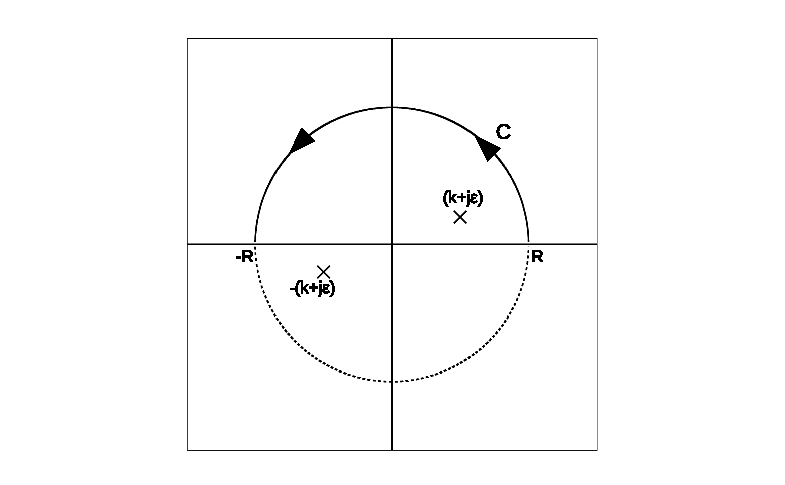
\includegraphics[width = 10cm]{./EPS/figure1new.eps}
    \label{fig1}
  \end{figure}
  \begin{eqnarray}
    F_+ = \int_{C} dk'\frac{e^{ik'(x-x')}}{(k'+k+i\epsilon)(k'-k-i\epsilon)} = \int_{-R}^Rdk' f_+(k') + \int_{C_1}dk'f_+(k')\label{c-int}
  \end{eqnarray}
  ただし
  \begin{eqnarray}
    f_+(k') = \frac{e^{ik'(x-x')}}{(k'+k+i\epsilon)(k'-k-i\epsilon)}
  \end{eqnarray}
  ここで留数定理
  \begin{eqnarray}
    \int_Cdz f(z) = 2\pi i\sum_j R(a_j)
  \end{eqnarray}
  を用いる. 極を$a_j$, Laurent展開における$(z-a)^{-n}$の係数を$R(a)$としている.今回の積分には1位の極しか含まれていないのでLaurent展開は
  \begin{eqnarray}
    R(a) = \lim_{z \rightarrow a}(z-a)f(z)
  \end{eqnarray}
  で与えられる. 以上より, (\ref{c-int})は
  \begin{eqnarray}
    F_+ &=& 2\pi i\lim_{k' \rightarrow k + j\epsilon }\left[(k'-k-j\epsilon)\frac{e^{ik'(x-x')}}{(k'+k+i\epsilon)(k'-k-i\epsilon)}\right]\\
    &=& \pi i\frac{e^{i(x-x')(k+j\epsilon)}}{k+j\epsilon}
  \end{eqnarray}
  と計算できる. さらに
  \begin{eqnarray}
    \lim_{R\rightarrow\infty}\int_{C_1}dk'f_+(k') =0
  \end{eqnarray}
  であることはすぐにわかる. 以上から
  \begin{eqnarray}
    G^\epsilon_+(x, x') &=& -\frac{1}{2\pi}\pi i\frac{e^{i(x-x')(k+j\epsilon)}}{k+j\epsilon}\\
    \therefore G_+(x, x') &=& \lim_{\epsilon\rightarrow 0}G_+^\epsilon(x, x') = -\frac{i}{2k}e^{ik(x-x')}
  \end{eqnarray}
  のように, Green関数を具体的に計算できた.\\
\item[ii)] $x<x'$の場合    
  \begin{figure}[htbp]
    \centering
    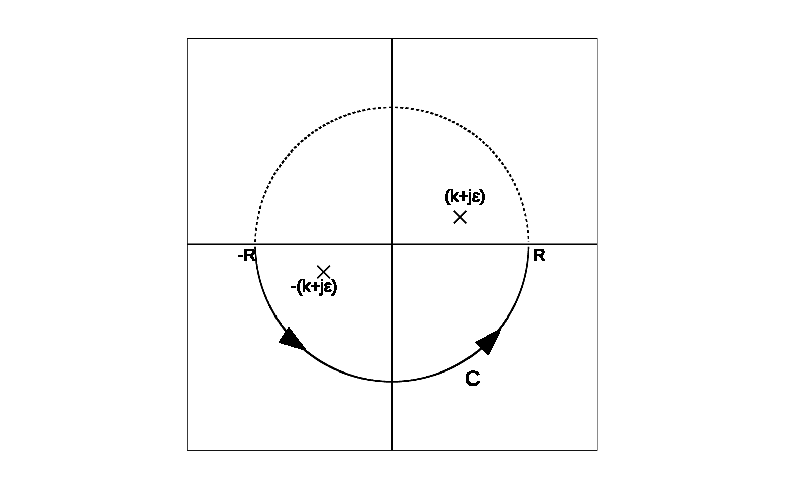
\includegraphics[width = 10cm]{./EPS/figure2new.eps}
    \label{fig2}
  \end{figure}
  先程と同様の計算より,
  \begin{eqnarray}
    G_-(x, x') = -\frac{i}{2k}e^{-ik(x-x')}
  \end{eqnarray}
  となる. 
\end{itemize}
まとめると,
\begin{eqnarray}
  G_\pm(x, x') = -\frac{i}{2k}e^{\pm ik(x-x')}
\end{eqnarray}
グリーン関数が求まったので, これを用いて波動関数を求める. 波動関数の摂動展開は
\begin{eqnarray}
  \psi(x) = \psi_0(x) + \int dx'G_+(x, x')H_p(x')\psi(x')
\end{eqnarray}
と表される.$\psi_0(x)$は非摂動解なので平面波であり, $H_p$はポテンシャルである. つまり, 領域ごとに$H_p$を変えてこの積分を計算すれば良い.
\section{場の理論におけるGreen関数}
場の理論と書きましたが, 以下では第二量子化された量子力学\footnote{「第二量子化された量子力学」と「場の量子論」は明確に区別されるべきです. 量子力学はあくまでSchr\"odinger方程式によって真空(基底状態)が決まるが, 場の量子論では真空は理論を閉じるように選ぶものである. 第二量子化における真空は消滅演算子$a$が消去する状態で確定しますが, 場の量子論においては真空期待値$\bra{0}\psi\ket{0}$がゼロでない値を持つことが許されます. こういう構造がないと, 粒子が存在する状態を真空とするBECのような物理を記述できなくなります.}におけるGreen関数についてまとめます.
\subsection{時間依存自由粒子Green関数}
場の演算子$\psi(\bm{x}, t)$はSchr\"odinger方程式
\begin{eqnarray}
  \left(i\hbar\partial_t -H\right)\psi(\bm{x}, t) = 0
\end{eqnarray}
で記述される. 今までの1粒子波動関数と同様に, 非摂動部のGreen演算子は
\begin{eqnarray}
  G_0(\bm{x}, t) = \left(i\hbar\partial_t -H_0\right)^{-1}
\end{eqnarray}
と表せ, グリーン関数は
\begin{eqnarray}
  \left(i\hbar\partial_t -H_0\right)G_0(\bm{x}, \bm{x}'; t, t') = \delta(t-t')\delta(\bm{x} - \bm{x}')
\end{eqnarray}
である. この微分方程式の解は2つ存在する:
\begin{eqnarray}
  G_0^R(k, \tau) &=& -i\theta(\tau)e^{-iE_k\tau}\hspace{1cm}\tau = t-t'\\
  G_0^A(k, \tau) &=& i\theta(\tau)e^{-iE_k\tau}\hspace{1cm}\tau = t'-t
\end{eqnarray}
$G^R$を遅延グリーン関数, $G^A$を先進グリーン関数と呼ぶ. 現象が時間に対して未来に進むのが遅延グリーン関数, 過去に進むのが先進グリーン関数になっている\footnote{数学的には時間が反転するような解を持っていてもおかしくないし, むしろ持っているべき. 時間発展がユニタリーなら解は時間反転対称性がある. }. 因果律を考慮しなくて良い場合であればどちらを用いてもよいが, 遅延グリーン関数の方が物理的な直感と合致している.
\subsection{相関関数と温度Green関数}
系が熱平衡状態にあるとき, $t = 0$の基底状態$\ket{\psi(0)}$を用いてGreen関数は, 可観測量$A, B$の時間相関関数で与えられる\footnote{Green関数が系に何かしらの揺動を与えた時の応答と解釈するなら自然な定義と言える.}:
\begin{eqnarray}
  G(t-t') \equiv \expval{\expval{A(t)B(t')}} = -i\bra{\psi(0)}{\rm T}[A(t)B(t')]\ket{0}
\end{eqnarray}
$A(t), B(t')$はHeisenberg描像, ${\rm T}[\ ]$は時間順序積. T積は因果律を守るために導入されている.

有限温度系における期待値は
\begin{eqnarray}
  \expval{A} = \frac{{\rm Tr}Ae^{-\beta H}}{{\rm Tr}e^{-\beta H}}
\end{eqnarray}
で与えられるので, 上のGreen関数は
\begin{eqnarray}
  G(t-t') &=& -i\frac{{\rm T}[{\rm Tr}A(t)B(t')e^{-\beta H}]}{{\rm Tr}e^{-\beta H}}\\
  &=& -i\frac{{\rm T}[{\rm Tr}e^{iHt/\hbar}Ae^{-iHt/\hbar}e^{iHt/\hbar}Be^{-iHt/\hbar}e^{-\beta H}]}{{\rm Tr}e^{-\beta H}}\\
  &=& -i\frac{{\rm T}[{\rm Tr}e^{iHt/\hbar}ABe^{-(it/\hbar + \beta)H}]}{{\rm Tr}e^{-\beta H}}
\end{eqnarray}
これを温度Green関数(松原Green関数)と呼ぶ.
\newpage
\chapter{超伝導}
超伝導の現象論であるGinzburg-Landau理論とBCS理論を扱う. 
\section{超電導の基礎}
\subsection{超電導体の性質}
\begin{itemize}
\item 電気抵抗ゼロ
\item 磁束の侵入を許さない (flux exclusion)
\item 磁束の排除が起こる (flux expulsion)
\end{itemize}
超伝導でない抵抗ゼロの金属ではflux expulsionはない.
\subsection{磁束の量子化}
磁束の量子化は超伝導の巨視波動関数$\psi = \psi_0e^{i\theta}$の一価性の要請から導かれる.
\begin{eqnarray}
  \nonumber  \bm{J}_s &=& \frac{e}{2m}\frac{\hbar}{i}(\psi^*\nabla) - \frac{e^2}{m}|\psi|^2\bm{A}\\
  &=& -\frac{e}{m}|\psi|^2(\hbar\nabla\theta + e\bm{A})
\end{eqnarray}
$\bm{J}_s ~ n_se\bm{v}_s = |\psi|^2e\bm{v}_s$であることに着目すると
\begin{eqnarray}
  \nabla\theta = -\frac{m}{\hbar}\bm{v}_s - \frac{e}{\hbar}\bm{A}
\end{eqnarray}
となる. 波動関数の一価性が保証されるには, 閉曲面$C$に沿って線積分したものが$2\pi$の整数倍でなければならない:
\begin{eqnarray}
  \int_C dl \nabla\theta = \int_C dl \bm{v}_s = 2\pi n
\end{eqnarray}
循環が量子化されている.
\section{超伝導の現象論 : Ginzburg-Landau理論}
超伝導を現象論的にモデル化したGinzburg-Landau理論について. 
\subsection{相転移とOder parameter}
ハミルトニアンが
\begin{eqnarray}
  H = -2\sum_{i,j}J\bm{s}_i\cdot\bm{s}_j
\end{eqnarray}
と書けるようなスピン相互作用を考える. これをハイゼンベルグ模型という. 系の平衡状態はHelmholtz自由エネルギー
\begin{eqnarray}
  F = U -TS
\end{eqnarray}
を最小にするように決まる. 低温($T<\!<U/S$)ならば内部エネルギー$U=\expval{H}$がleadingであり, これを最小化するようにスピンの向きが揃う. これを強磁性体と呼ぶ.  一方で高温ならばエントロピーの項が優勢なのでエントロピーが最大になるようにスピンの向きがバラバラになる. これを常磁性体と呼ぶ.

スピンの向きが揃うときに真空期待値が値を持ち, これを秩序変数と呼ぶ. 秩序変数がゼロでない値に変化するとき, これを相転移と呼ぶ.
\subsection{Ginzburg-Landau方程式}
自由エネルギーを秩序変数$\psi$の冪で展開:
\begin{eqnarray}
  {\cal F}[\psi] = {\cal F}_0 + \alpha|\psi|^2 + \frac{\beta}{2}|\psi|^4
\end{eqnarray}
ここで$\alpha = a(T-T_C)$である. 自由エネルギーの最小を与える$|\psi|$は微分すれば
\begin{eqnarray}
  |\psi| =
  \begin{cases}
    \hspace{1cm}0&(T>T_C)\\
    \\
    \sqrt{\cfrac{a(T_C-T)}{\beta}}&(T<T_C)
  \end{cases}
\end{eqnarray}
と求められる. そもそも$|\psi| = M$(磁化)と考えるのが自然で, なおかつ時間反転対称性を持っているので$M$の奇数次はない. $\alpha<0$のときに$|\psi| = 0$以外の極値を持つようになる. $\alpha(T) = a(T-T_C)$とすれば相転移を記述できる.

$\psi$が空間一様でない, つまり$\psi$が$r$依存性を持つ場合は
\begin{eqnarray}
  {\cal F} &=& {\cal F}_0 + \int d\bm{r} f(\bm{r})\\
  &=& {\cal F}_0 + \int dV\left[\alpha|\psi(\bm{r})|^2 + \frac{\beta}{2}|\psi(\bm{r})|^4\right]  
\end{eqnarray}
と書くことにする. 外部磁場などがある場合, 粒子の運動エネルギ^による補正項を加えなければならない:
\begin{eqnarray}
  \int dV \frac{\hbar^2}{2m}|\nabla\psi(\bm{r})|^2
\end{eqnarray}
自由エネルギーにはゲージ対称性があるので, ゲージ変換に対して不変な形で導入しなければならない:
\begin{eqnarray}
  {\cal F} &=& {\cal F}_0 + \int dV\left[\frac{\hbar^2}{2m}\left|\left(\nabla - \frac{ie}{\hbar}\bm{A}(\bm{r}))\psi(\bm{r}\right)\right|^2 + \alpha|\psi(\bm{r})|^2 + \frac{\beta}{2}|\psi(\bm{r})|^4 + \frac{\mu_0}{2}(\nabla\times\bm{A})^2\right]
\end{eqnarray}
これの変分がゼロになるところを探す:
\begin{eqnarray}
  \nonumber  \delta{\cal F} &=&\int dV\left[-\frac{\hbar^2}{2m}\left(\nabla - \frac{ie}{\hbar}\bm{A}(\bm{r})\right)^2\psi(\bm{r}) + \alpha\psi(\bm{r}) + \beta|\psi(\bm{r})|^2\psi(\bm{r})\right]\delta\psi^*(\bm{r})\\
  &+&\int \left[\frac{\hbar^2}{2m}\left(\nabla - \frac{ie}{\hbar}\bm{A}(\bm{r})\right)\psi(\bm{r})\right]\delta\psi^*(\bm{r})\cdot d\bm{S}
\end{eqnarray}
右辺第一項の被積分関数がゼロになることから
\begin{eqnarray}
  \left[-\frac{\hbar^2}{2m}\left(\nabla - \frac{ie}{\hbar}\bm{A}(\bm{r})\right)^2 + \alpha + \beta|\psi(\bm{r})|^2\right]\psi(\bm{r}) = 0\label{GL}
\end{eqnarray}
を得る. これが秩序変数を記述するGinzburg-Landau(GL)方程式である. ちなみに今回は${\cal F}$について$\psi$の変分を取ったが, $A$についての変分を取るとアンペールの法則が出てくる.
\subsection{ゲージ変換の復習}
\subsubsection{Maxwell方程式}
電磁気学におけるゲージ変換のおはなし. Maxwell方程式
\begin{eqnarray}
  {\rm rot} \bm{E} + \frac{\partial\bm{B}}{\partial t} &=& 0\hspace{2cm}(ファラデーの法則)\\
  {\rm rot} \bm{B} - \varepsilon_0\mu_0\frac{\partial \bm{E}}{\partial t} &=& \mu_0 \bm{i}\hspace{2cm}(アンペールの法則)\\
  {\rm div} \bm{E} &=& \frac{\rho}{\varepsilon_0}\hspace{2cm}(電荷のガウスの法則)\\
  {\rm div} \bm{B} &=& 0\hspace{2cm}(電荷のガウスの法則)
\end{eqnarray}
について. $\bm{B} = {\rm rot}\bm{A}$という仮定をすると${\rm div}\bm{B} = {\rm div\ rot}\bm{A} = 0$という関係が自明に出てくる(ただし, これは$\bm{A}$に特異点がない場合). この仮定をファラデーの法則に代入:
\begin{eqnarray}
  {\rm rot}(\bm{E} + \frac{\partial \bm{A}}{\partial t}) = 0
\end{eqnarray}
もし
\begin{eqnarray}
  \bm{E} + \frac{\partial \bm{A}}{\partial t} = -{\rm grad}\phi \hspace{0.5cm}\Longrightarrow\hspace{0.5cm} \bm{E} = -{\rm grad}\phi - \frac{\partial \bm{A}}{\partial t}
\end{eqnarray}
という仮定をすればファラデーの法則も自明となる. $\phi$と$A$が導入できればMaxwell方程式がとてもカンタンになる. $\phi$と$A$をまとめて電磁ポテンシャルと呼ぶ. 新しい方程式は
\begin{eqnarray}
  \left(\nabla^2 - \varepsilon_0\mu_0\frac{\partial^2}{\partial t^2}\right)\bm{A} - {\rm grad}\left({\rm div}\bm{A} + \varepsilon_0\mu_0\frac{\partial \phi}{\partial t}\right) &=& -\mu_0\bm{i}\label{max1}\\
  \nabla^2\phi + {\rm div}\frac{\partial \bm{A}}{\partial t} &=& -\frac{\rho}{\varepsilon_0}\label{max2}
\end{eqnarray}
となる.ここで
\begin{eqnarray}
  \bm{A}' = \bm{A} + {\rm grad}\chi
\end{eqnarray}
という量を定義しても, 磁束密度$\bm{B}$は変わらない. その代わり電場は変わってしまうので
\begin{eqnarray}
  \phi' = \phi - \frac{\partial \chi}{\partial t}
\end{eqnarray}
を導入すると全て辻褄が合う. この$(\phi, \bm{A})\mapsto(\phi', \bm{A}')$の変換をゲージ変換と呼び, Maxwell方程式はゲージ不変性を持つ.
\subsubsection{ローレンツゲージ}
(\ref{max1})(\ref{max2})には各々$\phi, \bm{A}$が含まれているので計算がめんどくさい. せめて
\begin{eqnarray}
  {\rm div}\bm{A} + \varepsilon_0\mu_0\frac{\partial \phi}{\partial t} = 0\label{max3}
\end{eqnarray}
となってくれれば(\ref{max1})は
\begin{eqnarray}
  \left(\nabla^2 - \varepsilon_0\mu_0\frac{\partial \phi}{\partial t}\right)\bm{A} = -\mu_0\bm{i}\label{max4}
\end{eqnarray}
のように$\bm{A}$だけの式になり, (\ref{max3})を(\ref{max2})に代入すると
\begin{eqnarray}
  \left(\nabla^2 - \varepsilon_0\mu_0\frac{\partial^2}{\partial t^2}\right)\phi &=& -\frac{\rho}{\varepsilon_0}
\end{eqnarray}
という対称性のとてもよい形になる. (\ref{max3})をローレンツ条件という.
\begin{itembox}[c]{ローレンツゲージにおけるMaxwell方程式}
  \begin{eqnarray}
    \nonumber    \left(\nabla^2 - \varepsilon_0\mu_0\frac{\partial \phi}{\partial t}\right)\bm{A} &=& -\mu_0\bm{i}\\
    \nonumber    \left(\nabla^2 - \varepsilon_0\mu_0\frac{\partial^2}{\partial t^2}\right)\phi &=& -\frac{\rho}{\varepsilon_0}
  \end{eqnarray}
  ただし
  \begin{eqnarray}
    \nonumber    {\rm div}\bm{A} + \varepsilon_0\mu_0\frac{\partial \phi}{\partial t} = 0
  \end{eqnarray}
\end{itembox}
\begin{eqnarray}
  (\phi, \bm{A})\mapsto(\phi', \bm{A}') \Longrightarrow
  \begin{cases}
    \bm{A}' = \bm{A} + {\rm grad}\chi\\
    \phi' = \phi - \cfrac{\partial \chi}{\partial t}
  \end{cases}
\end{eqnarray}

がローレンツ条件(\ref{max3})を満たすような$\chi$が存在すれば, この以上の変形が正当化される. ローレンツゲージによるMaaxwell方程式はローレンツ共変である. 
\subsubsection{クーロンゲージ}
ローレンツ条件に対して
\begin{eqnarray}
  {\rm div}\bm{A} = 0
\end{eqnarray}
という条件を課すと, クーロンの法則と等価なポアソン方程式が導かれることからこれをクーロン条件(クーロンゲージ)と呼ぶ.
\begin{itembox}[c]{クーロンゲージにおけるMaxwell方程式}
  \begin{eqnarray}
    \nonumber   && \nabla^2\phi = -\frac{\rho}{\varepsilon_0}\\
    \nonumber    &&\nabla^2\bm{A} -\varepsilon_0\mu_0\frac{\partial^2 \bm{A}}{\partial t^2} - \varepsilon_0\mu_0\frac{\partial}{\partial t}{\rm grad}\phi = \mu_0\bm{i}
  \end{eqnarray}
  ただし
  \begin{eqnarray}
    \nonumber    {\rm div}\bm{A} = 0
  \end{eqnarray}
\end{itembox}
クーロンゲージはローレンツ共変ではなくあまり方程式の対称性は良くないが, 電磁場の量子化などでは便利なので用いられることがある.
\subsection{GLコヒーレンス長と侵入長}
外部磁場がない場合の一次元GL方程式(\ref{GL})を境界条件$\psi(0) = 0$のもとで解く:
\begin{eqnarray}
  \left[-\frac{\hbar^2}{2m}\frac{d^2}{dx^2} + \alpha + \beta|\psi(x)|^2\right]\psi(x) = 0  
\end{eqnarray}
これは$x = 0$の境界には超伝導体はなく, $x > 0$を超電導体で占められているような状況である. コヒーレンス長$/xi$を
\begin{eqnarray}
  \xi^2 = \frac{\hbar^2}{2m|\alpha|}
\end{eqnarray}
と定義する. 超伝導状態では$\alpha < 0$である\footnote{こうしないとGLヘルムホルツエネルギーが$\psi>0$の領域で最小値を持たなくなる.}. 両辺を$\psi_0 = \sqrt{|\alpha|/\beta}$を用いて整理して
\begin{eqnarray}
  -\frac{d^2\psi}{dx^2} - \psi + \psi^3 = 0
\end{eqnarray}
を得る. 左辺に$2\frac{d\psi}{dx}$を掛ける:
\begin{eqnarray}
  2\frac{d\psi}{dx}\left[-\frac{d^2\psi}{dx^2} - \psi + \psi^3\right] = 0
\end{eqnarray}
ここで
\begin{eqnarray}
  \frac{d}{dx}\left(\frac{d\psi}{dx}\right)^2 = 2\frac{d\psi}{dx}\left(\frac{d^2\psi}{dx^2}\right), \hspace{0.5cm}\frac{d\psi^2}{dx} = 2\psi\frac{d\psi}{dx}, \hspace{0.5cm}\frac{d\psi^4}{dx} &=& 4\psi^3\frac{d\psi}{dx}
\end{eqnarray}
を用いて変形する:
\begin{eqnarray}
  \frac{d}{dx}\left[-\xi^2\left(\frac{d\psi}{dx}\right)^2-\psi^2 + \frac{1}{2}\psi^4\right] = 0
\end{eqnarray}
微分がゼロなので微微分関数は定数:
\begin{eqnarray}
  -\xi^2\left(\frac{d\psi}{dx}\right)^2-\psi^2 + \frac{1}{2}\psi^4 = A\ ({\rm const})
\end{eqnarray}
また, 境界条件$d\psi/dx\rightarrow 0, \psi\rightarrow 1\ (x\rightarrow+\infty)$を課すと$A = -\frac{1}{2}$であることがわかる. これにより
\begin{eqnarray}
  \xi^2\left(\frac{d\psi}{dx}\right)^2 = \frac{1}{2}\left(1-\psi^2\right)
\end{eqnarray}
という方程式が得られる.

これは非線形微分方程式だが特解を持っている:
\begin{eqnarray}
  \psi(x) = \tanh(\frac{x}{\sqrt{2\xi}})
\end{eqnarray}
これはソリトン解と呼ばれる. $x = 0$で強制的にゼロにされた$\psi$が$\xi$程度で回復している.また
\begin{eqnarray}
  \xi = \left(\frac{\hbar^2}{2m|\alpha|}\right)^{\frac{1}{2}} = \left(\frac{\hbar^2}{2ma(T-T_C)}\right)^{\frac{1}{2}} = \left(\frac{\hbar^2}{2maT_C}\right)^{\frac{1}{2}}\left(1 - \frac{T}{T_C}\right)^{\frac{1}{2}}
\end{eqnarray}
$T\rightarrow T_C\ (T_C > T)$でコヒーレンス長は発散していく自然な結果が得られる.
\subsection{ソリトンの特徴}
普通の線形波なら波動方程式で記述される異なる波長を持つ波の重ね合わせで記述できる. 異なる波長の波は$v = f\lambda$に従って伝搬速度も異なるので, 波束は次第に崩壊していく(分散が発散していく). しかしソリトンはある非線形微分方程式の定常解なので形を変えずに伝搬していき, 波束も崩壊しない.
\section{超伝導の微視的理論 : Bardeen-Cooper-Schrieffer理論}
\subsection{金属の基本性質}
一辺$L$の箱に閉じ込められた自由電子について考える. 周期境界条件を課すと, 波動関数は平面波で記述できる:
\begin{eqnarray}
  \psi_{\bm{k}}(\bm{r}) = \frac{1}{\sqrt{L^3}}e^{i\bm{k}\cdot\bm{r}}
\end{eqnarray}
エネルギー分散関係は
\begin{eqnarray}
  \varepsilon_{\bm k} = \frac{\hbar^2k^2}{2m}
\end{eqnarray}
である. ここで波数は
\begin{eqnarray}
  k_i = n_i\left(\frac{2\pi}{L}\right)\hspace{0.5cm}(i= x, y, z)
\end{eqnarray}
で与えられる. 3次元$k$空間の単位体積$(2\pi/L)^3$あたりに1つ(スピン自由度を考えると2つ)の状態が入れる. 下の準位から埋めていくと, 状態が埋まった空間は球になる. これをフェルミ球と呼び, その境界をフェルミ面と呼ぶ. フェルミ面の半径を$k_F$とすると
\begin{eqnarray}
  N = 2\left(\frac{L}{2\pi}\right)^3\times\frac{4}{3}\pi k_F^3
\end{eqnarray}
である. 電子密度を$n = N/L^3$とすると
\begin{eqnarray}
  k_F = (3\pi n)^{\frac{1}{3}}
\end{eqnarray}
となる. エネルギー$\varepsilon$の状態を電子が占める確率はFermi-Dirac分布関数
\begin{eqnarray}
  f(\varepsilon) = \frac{1}{\exp[(\varepsilon- \varepsilon_F)/k_BT]+1}
\end{eqnarray}
で与えられる.
\subsection{電子-格子間相互作用}
電子と金属イオンの間の相互作用は電子がイオン構造を歪めるという描像で理解される\footnote{金属イオン中に電子があると電子と金属イオンが引力相互作用で近づき合い, 金属イオンの配列が微妙に歪むことになる. この電子が金属中を移動すると, 金属イオンの配列の歪みも一緒に伝搬していくように見える. これが格子振動であり, これを量子化するとフォノンになる. さて, この場合は電子の運動エネルギーが格子振動に一部持って行かれることになり, これが電気抵抗の由来になる. しかし, この電子の近くに別の電子がある場合は, 格子振動により正電荷密度が大きくなっているところからさらに引力相互作用を受けて加速することができる. つまり, ある電子が創りだした格子振動エネルギーを別の電子が受け取る, というメカニズムである. もちろんこれば古典的な描像であり, 全ての格子振動エネルギーが別の電子に引き継がれることは一見なさそうだが, 格子振動を量子化したフォノンであればdescreteなエネルギーのやりとりしかできないことになるので, 電子がフォノンのやりとりをすることでエネルギーの散逸を防ぐ枠組みを正当化することができそうである. このフォノンのやり取りをする電子の組をCooper-pairという. }. つまり, 電子がフォノンを放出して異なる波数を持つモードへ遷移する, という描像である. フォノンを介した2電子間相互作用とは, 波数$k_1, k_2$の電子が$k_1 - q, k_2 + q$となる過程である.

\begin{figure}[htbp]
  \begin{minipage}{0.5\hsize}
    \centering
    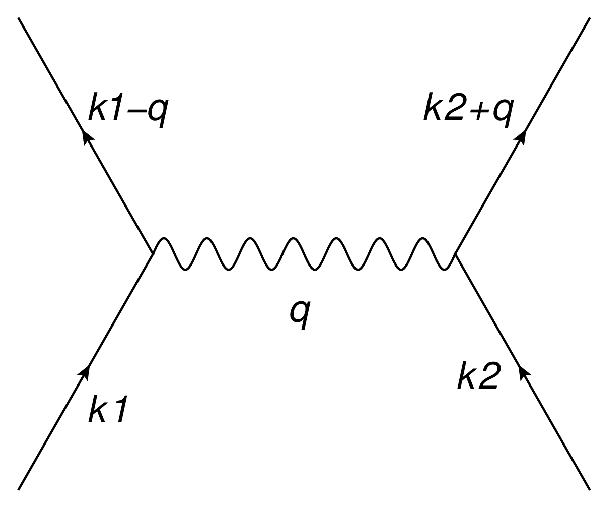
\includegraphics[width = 5.5cm]{./EPS/newdiagram1.eps}
    \figcaption{$\bm{k}_1$がフォノン$\bm{q}$を放出する過程}
    \label{diagram1}
  \end{minipage}
  \begin{minipage}{0.5\hsize}
    \centering
    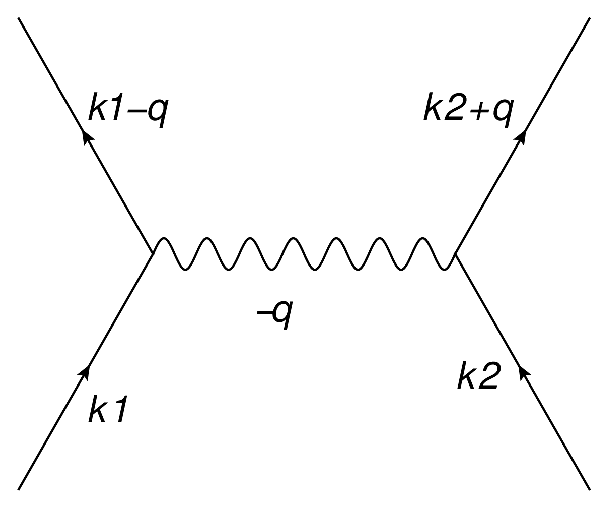
\includegraphics[width = 5.5cm]{./EPS/newdiagram2.eps}
    \figcaption{$\bm{k}_1$がフォノン$\bm{-q}$を吸収する過程}
    \label{diagram2}
  \end{minipage}
\end{figure}
フォノンを介した相互作用ハミルトニアンを$H'$とすると, エネルギーの2次摂動は
\begin{itemize}
\item 同じ電子がフォノンを放出して吸収した場合は自己エネルギー
\item 異なる電子同士がフォノンのやりとりをした場合は相互作用
\end{itemize}
を表すことになる. さて, 上の2種類の過程を考慮すると相互作用項の期待値は
\begin{eqnarray}
  U_2 &=& \sum_m\frac{\bra{f}H'\ket{m}\bra{m}H'\ket{i}}{E_i-E_m}\\
  E_i &=& \varepsilon_{\bm{k}_1} +\varepsilon_{\bm{k}_2}\\
  E_m &=&
  \begin{cases}
    \varepsilon_{\bm{k}_1 - \bm{q}} +\varepsilon_{\bm{k}_2} + \hbar\omega_{\bm{q}}\\
    \varepsilon_{\bm{k}_1} +\varepsilon_{\bm{k}_2 + \bm{q}} + \hbar\omega_{\bm{q}}
  \end{cases}
\end{eqnarray}
より
\begin{eqnarray}
  U_2 &=& \frac{|V_{\bm q}|^2}{\varepsilon_{\bm{k}_1 - \bm{q}} +\varepsilon_{\bm{k}_1} + \hbar\omega_{\bm{q}}} + \frac{|V_{\bm q}|^2}{\varepsilon_{\bm{k}_2} +\varepsilon_{\bm{k}_2 + \bm{q}} + \hbar\omega_{\bm{q}}}\\
  &=& \frac{2|V_{\bm q}|\hbar\omega_{\bm q}}{(\varepsilon_{\bm{k}_1 - \bm{q}} +\varepsilon_{\bm{k}_1})^2-(\hbar\omega_{\bm q})^2}
\end{eqnarray}
となる. ここではエネルギー保存則を用いた. $|\varepsilon_{\bm k} - \varepsilon_{\bm k-q}| <\!< \hbar\omega_{\bm q}$であれば電子間相互作用は引力となる. つまり, フェルミ面上の電子間にはフォノンを介した引力相互作用が働く可能性がある.
\subsection{Cooper問題}
次に問題になるのが, 「フェルミ面直上にある2つの電子間相互作用を考えるとき, この電子対が束縛状態を作るか」ということ. 言い換えると, 「いかに弱くても引力相互作用があれば電子対の束縛状態が実現するかどうか」. 着目する2電子の波動関数を
\begin{eqnarray}
  \Psi(\bm{r}_1, \sigma_1, \bm{r}_2, \sigma_2) = \psi(\bm{r}_1, \bm{r}_2)\chi(\sigma_1, \sigma_2)
\end{eqnarray}
とする. $\psi$が満たすのはScr\"odinger方程式
\begin{eqnarray}
  &&\bqty{-\frac{\hbar^2}{2m}\pqty{\nabla^2_1 + \nabla^2_2} + V(\bm{r}_1, \bm{r}_2)}\psi(\bm{r}_1, \bm{r}_2) = E\psi(\bm{r}_1, \bm{r}_2)\\
  &&\chi(\sigma_1, \sigma_2) = \frac{1}{\sqrt{2}}\pqty{\ket{\uparrow}\ket{\downarrow} - \ket{\downarrow}\ket{\uparrow}}
\end{eqnarray}
重心・相対座標$\bm{R} = \pqty{\bm{r}+\bm{r}}/2,\ \bm{r} = \bm{r}_1 - \bm{r}_2$を用いて
\begin{eqnarray}
  \psi(\bm{r}_1,\bm{r}_2) = \varphi(\bm{r})e^{i\bm{KR}}
\end{eqnarray}
\newpage
\chapter{Anderson局在とその周辺}
\section{Anderson局在とは}
不純物がある系において, Drudeの電子論などでは説明できない電気伝導度が実験的に確かめられた. 具体的には, Drudeモデルでは電気伝導度は平均自由行程に比例するはずだが, ある点を境に相転移のごとく電気伝導度が落ち込む結果が得られた\footnote{Anderson転移と呼ぶ}.

Andersonはこの不純物による電子の局在という問題に対して新しい理論を作った.
\section{P.W.Anderson. Phys. Rev. $\bm{109}$, 1492(1958)}
\subsection{Tight-Binding近似}
電子が規則正しい格子の上にある場合を考える. このとき電子の波動関数は原子軌道$\phi$の相対座標表示を用いて
\begin{eqnarray}
  \ket{\psi_{\bm{k}}(\bm{r})} = \sum_{\bm{R}}e^{i\bm{k}\cdot\bm{R}}\ket{\phi_0(\bm{r}-\bm{R})}
\end{eqnarray}
のように展開できる\footnote{ケットの中に位置依存性$\bm{r}$を入れる不自然さには目を瞑る方向で}. 展開係数はBroch条件を守るために平面波になっている. これがTB近似\footnote{LCAO近似とも}である.

今回は不純物が混じった系を考えるので展開系数は平面波ではない:
\begin{eqnarray}
  \ket{\psi_{\bm{k}}(\bm{r})} = \sum_{\bm{R}}a_{\bm R}^{\bm r}\ket{\phi_0(\bm{r}-\bm{R})}
\end{eqnarray}
これを各格子点のインデックスごとに和を取ることを考えて以下のように簡略化した記号を導入する:
\begin{eqnarray}
  \sum_{\bm{R}}a_{\bm R}^{\bm r}\ket{\phi_0(\bm{r}-\bm{R})} = \sum_ja_j\ket{j}
\end{eqnarray}
Schr\"odinger方程式は以下のようになる:
\begin{eqnarray}
  H\ket{\psi} &=& \qty(H_{\rm atom} + \Delta V(\bm{r}))\ket{\psi}\\
  &=&\sum_j\epsilon_j\ket{j}a_j + \sum_j\Delta V(\bm{r})\ket{j}a_j
\end{eqnarray}
$\Delta V$は全ポテンシャルから孤立原始中で電子が感じるポテンシャルを引いたもの. これの右から$\bra{i}$を作用させると
\begin{eqnarray}
  \bra{i}H\ket{\psi} = \epsilon_ia_i + \sum_jV_{ij}a_j
\end{eqnarray}
となる. $V_{ij} = \bra{i}\Delta V({\bm r})\ket{j}$であり, $\bra{i}\ket{j} \simeq \delta_{ij}$であることを用いている. 以上からハミルトニアンは
\begin{eqnarray}
  H = \sum_i\epsilon_i\ket{i}\bra{i} + \sum_{i\neq j}V_{ij}\ket{i}\bra{j}
\end{eqnarray}
であることがわかる\footnote{量子力学・場の理論ではまずハミルトニアンがあり, そこからSchr\"odinger方程式やらHeisenberg方程式やらを導出することが多いが, 今回の文脈ではその逆を行っている. つまり波動関数を作り, その波動関数でSchr\"odinger方程式を作り, ハミルトニアンを推定している. 一見不思議に思えるがこのような議論は論文でもよく見かける. 理論がSelf-consistentであればどこからスタートするかは任意であるということか}.

これらを用いて時間依存Schr\"odinger方程式
\begin{eqnarray}
  i\hbar\frac{\partial \psi_t}{\partial t} = H\psi_t
\end{eqnarray}
を時間依存性を展開系数に押し付けた波動関数の展開
\begin{eqnarray}
  \psi_t = \sum_j a_j(t)\ket{j}
\end{eqnarray}
を用いて書き換える:
\begin{eqnarray}
  i\hbar\frac{\partial a_i(t)}{\partial t} = \epsilon_ia_i(t) + \sum_{j(\neq i)}V_{ij}a_j(t)\label{schroedinger-anderson}
\end{eqnarray}
\subsection{Andersonの理論}
初期時刻にあるサイト$i=0$に電子を一つ置いて時間発展させたとき, $a_i$が時刻$\infty$で有限の値を取る場合, 電子は局在していると言える. これを計算するために(\ref{schroedinger-anderson})をLaplace変換する:
\begin{eqnarray}
  i\qty[sf_j(s) - a_j(0)] &=& \epsilon_jf_j(s) + \sum_{k(\neq j)}V_{jk}f_k(s)\\
  f_j(s) &=& \frac{i\delta_{j0}}{is - \epsilon_j} + \sum_{k(\neq j)}\frac{1}{is - \epsilon_j}V{jk}f_k(s)
\end{eqnarray}
ここでは$\hbar = 1$の単位系を用いている. また$a_j(0) = \delta_{j0}$という性質も用いている. なぜこんなことをするのかというと, $sf(s)\rightarrow a_j(\infty)\ \ (s\rightarrow 0^+)$という性質があるから. $f_j(s)$から$a_j(\infty)$の情報が得られるのである.

この右辺第二項の$f_k$に逐次代入してき, $j = 0$を代入すると
\begin{eqnarray}
  \nonumber  f_0(s) &=&  \frac{i}{is - \epsilon_j} + \sum_k\frac{1}{is - \epsilon_0}V_{0k}\frac{1}{is - \epsilon_k}V_{k0}\frac{1}{is - \epsilon_0}\\
  &+& \sum_{k, m} \frac{1}{is - \epsilon_0}V{0k}\frac{1}{is - \epsilon_k}V_{km}\frac{1}{is - \epsilon_m}V_{m0}\frac{1}{is - \epsilon_0} + \cdots \label{anderson2}
\end{eqnarray}
となる. これは$j = 0$からスタートして様々な格子点を通過してまた$j = 0$に戻ってくる経路を全て足し合わせるような計算を行っている. その経路の中にはループを作るものも存在するが, 自己エネルギーは
\begin{eqnarray}
  {\cal L}_k(s) = \frac{1}{is - \epsilon_k - \varsigma}
\end{eqnarray}
というようにカウンター項$\varsigma$でくりこみが可能である. よってループのない経路のみを考えれば良い. また, コネクティビティが最近接サイト数$z$を用いて$z-2 < K \leq z - 1$と書けること, $P$ステップ後のコネクティビティが$K^P$で概算できることを用いて(\ref{anderson2})を摂動的に処理し, $a_i(\infty)$がゼロになるところと有限の値を取るところを解析したのがAndersonの1958年の論文である.

しかしこの取り扱いはなかなか難しい. これの見通しを良くするのがスケーリング理論である.
\section{E.Abrahams et al. Phys. Rev. Lett. $\bm{42}$, 673(1979)}
\newpage
\chapter{熱・統計・量子統計力学}
\section{熱力学}
\subsection{状態量}
系の状態のみで一意に決まり, 過去の履歴・経路に依らない(積分値が経路に依らない)ものを状態量と呼ぶ. 
\subsection{完全な熱力学関数}
系の平衡状態における熱力学的性質の情報を全て持っているものを完全な熱力学関数と呼ぶ. 示量性状態量. 系の情報を全て持っているというのは, 状態量がこの関数の偏微分で全て求まるということ. 例えば内部エネルギー$U(S, N, V)$を用いて
\begin{eqnarray}
  \partial_SU &=& T\\
  \partial_NU &=& \mu\\
  \partial_VU &=& -p
\end{eqnarray}
という状態量が求まる. 全微分は
\begin{eqnarray}
  dU = TdS -pdV + \mu dN
\end{eqnarray}
である. これを変形して
\begin{eqnarray}
  dS = \frac{1}{T}dU +\frac{p}{T}dV - \frac{\mu}{T} dN
\end{eqnarray}
となり, $S$は$U, V, N$を変数とする関数として表された時に完全な熱力学関数となる. 統計力学においては温度を定義するときに
\begin{eqnarray}
  \partial_US = \frac{1}{T}
\end{eqnarray}
という表式をしばしば用いる.
\subsection{自由エネルギー}
熱力学第二法則より, 系は自由エネルギーが減少する方向に遷移する. 
\subsubsection{ヘルムホルツ自由エネルギー}
等温下で仕事として取り出し可能なエネルギーを表す.ヘルムホルツエネルギーが極小値を取るとき, 系は熱平衡状態にある.

定義:
\begin{eqnarray}
  F(T, V, N) = U(S(T, V, N), V, N) -TS(T, V, N)
\end{eqnarray}
ここで現れるエントロピーは完全な熱力学関数ではない. 各変数による偏微分は
\begin{eqnarray}
  \partial_TF &=& -S\\
  \partial_VF &=& -p\\
  \partial_NF &=& \mu
\end{eqnarray}
である. 全微分は
\begin{eqnarray}
  dF = -S(T, V, N)dT -p(T, V, N)dV + \mu(T, V, N) dN
\end{eqnarray}
\subsubsection{ギブズ自由エネルギー}
等温等圧下で仕事として取り出し可能なエネルギーを表す. ヘルムホルツエネルギーとの違いは等圧条件の有無.

定義:
\begin{eqnarray}
  G(T, p, N) = U(S(T, p, N), p, N) -TS(T, p, N)
\end{eqnarray}
以下ヘルムホルツエネルギーと同様.
\section{統計力学}
\subsection{目的}
微視的状態の数をかぞえて巨視的状態を導く. 
\subsection{ミクロカノニカルアンサンブル}
\subsection{Langevin方程式}
ブラウン粒子の運動を記述する方程式としてLangevinが導入した.
\begin{eqnarray}
  M\frac{dv}{dt} = -\frac{v}{\mu} + F_{\rm ext} + R(t)\label{Langevin}
\end{eqnarray}
ここで$\mu$を移動度, $F_{ext}$をマクロな外力, $R(t)$をミクロなノイズとする. $R$が確率過程であるので, 初期条件を与えても$v$が決定論的に定まらない. 

速度をFourier変換する:
\begin{eqnarray}
  v(t) &=& \frac{1}{\sqrt{2\pi}}\int d\omega e^{-i\omega t}\tilde{v}(\omega)\label{v1}\\
  \tilde{v}(\omega) &=& \frac{1}{\sqrt{2\pi}}\int dt e^{i\omega t}v(t)\label{v2}
\end{eqnarray}
さらに速度の時間相関関数とそのFourier変換を定義する:
\begin{eqnarray}
  C_v(t) &=& \expval{v(t_0)v(t_0 + t)}\\
  \tilde{C}_v(\omega) &=& \frac{1}{\sqrt{2\pi}}\int dt'e^{i\omega't'}\expval{v(t_0)v(t_0+t')}
\end{eqnarray}
ここで$\tilde{v}^*(\omega) = \tilde{v}(-\omega)$が成立している. (\ref{v2})より
\begin{eqnarray}
  \expval{\tilde{v}(\omega)\tilde{v}^*(\omega')} &=& \frac{1}{2\pi}\int dtdt' e^{i\omega t-i\omega' t'}\expval{v(t)v(t')}\\
  &=&\frac{1}{2\pi}\int dtdt'\left|\det(J)\right| e^{i\omega t'}e^{i(\omega -\omega')t}\expval{v(t+t')v(t)}\\
  &=&\delta(\omega-\omega')\int dt'e^{i\omega' t'}\expval{v(t+t')v(t)}\\
  &=&\delta(\omega-\omega')I_v(\omega')
\end{eqnarray}
ただし
\begin{eqnarray}
  J =
  \begin{pmatrix}
    \cfrac{\partial(t+t')}{\partial t}&\cfrac{\partial(t+t')}{\partial t'}\\
    \cfrac{\partial t'}{\partial t}&\cfrac{\partial t'}{\partial t'}\\
  \end{pmatrix}\hspace{1cm} |\det(J)| = 1
\end{eqnarray}
である. この式から
\begin{eqnarray}
  I_v(\omega) = \int dtC_v(t)e^{i\omega t} = \tilde{C}(\omega)
\end{eqnarray}
がわかる. これをWiener-Khinchinの定理という. 相関関数とパワースペクトルはFourier変換を通して関係付けられる.$\tilde{R}(\omega)$についても同様のことが言える:
\begin{eqnarray}
  \tilde{R}(\omega) &=& \frac{1}{\sqrt{2\pi}}\int dt e^{i\omega t}R(t)\label{R2}\\
  \tilde{C}_R(\omega) &=& \frac{1}{\sqrt{2\pi}}\int dte^{i\omega t}\expval{R(t_0)R(t_0+t)}\\
  \expval{\tilde{R}(\omega)\tilde{R}^*(\omega')}&=& \tilde{C}_R(\omega')\delta(\omega-\omega') 
\end{eqnarray}

以降$F_{\rm ext} = 0$のもとでLangevin方程式の解析をする. (\ref{Langevin})に(\ref{v1})を代入:
\begin{eqnarray}
  M\frac{d}{dt}\int d\omega e^{-i\omega t}\tilde{v}(\omega) &=& \int d\omega e^{-i\omega t}\left(-\frac{\tilde{v}(\omega)}{\mu} + \tilde{R}(\omega)\right)  \\
  \Longleftrightarrow M(-i\omega)\tilde{v}(\omega) &=&  -\frac{\tilde{v}(\omega)}{\mu} + \tilde{R}(\omega)
\end{eqnarray}
$\gamma = (M\mu)^{-1}$とすると
\begin{eqnarray}
  \tilde{v}(\omega) = \frac{1}{-i\omega + \gamma}\frac{\tilde{R}(\omega)}{M}
\end{eqnarray}
であることがわかる. 時間相関関数は
\begin{eqnarray}
  \tilde{C}_v(\omega) &=& \int d\omega' \expval{\tilde{v}(\omega)\tilde{v}^*(\omega')} = \frac{1}{(-i\omega + \gamma)(i\omega' + \gamma)M^2}\int d\omega' \expval{R(\omega)R^*(\omega')}\\
  &=& \frac{1}{(-i\omega + \gamma)(i\omega' + \gamma)M^2}\int d\omega' \tilde{C}_R(\omega')\delta(\omega-\omega') = \frac{1}{\omega^2 + \gamma^2}\frac{\tilde{C}_R(\omega)}{M^2}
\end{eqnarray}
$R$の確率過程の性質が与えられてパワースペクトル$C_R$が定まると速度$v$の相関関数やパワースペクトルが決定される. $R$がホワイトノイズだと仮定すると,
\begin{eqnarray}
  C_R(t) = \expval{R(t_0+t)R(t_0)} = C_R\delta(t)\\
  \tilde{C}_R(\omega) = \int dt e^{-i\omega t}C_R(t) = C_R
\end{eqnarray}
ということで, $\tilde{C}_R$は$\omega$によらない定数になる. このようなノイズを仮定すると, 速度相関関数は
\begin{eqnarray}
  C_v(t) = \int d\omega e^{-i\omega t}\tilde{C}_v(\omega) = \int d\omega \frac{C_Re^{-i\omega t}}{M^2(\omega^2 + \gamma^2)}
\end{eqnarray}
この積分を実行するために複素積分の応用を用いる:
\begin{eqnarray}
  \int_C dz \frac{C_Re^{-izt}}{M^2(z^2 + \gamma^2)} = \int_{C_1} \frac{C_Re^{-izt}}{M^2(z^2 + \gamma^2)} + \int_{-R}^R \frac{C_Re^{-izt}}{M^2(z^2 + \gamma^2)}
\end{eqnarray}
\begin{figure}[htbp]
  \centering
  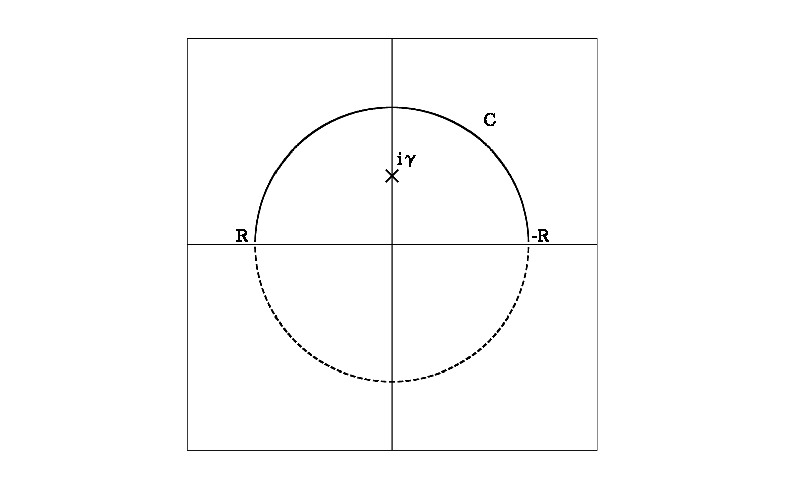
\includegraphics[width = 10cm]{./EPS/figure3new.eps}
  \label{fig3}
\end{figure}\\
極は$\omega = \pm i\gamma$で一位の極. 積分経路は上半円とする. 留数定理より
\begin{eqnarray}
  R(i\gamma) = \lim_{z\rightarrow i\gamma}(z - i\gamma)f(z) = \frac{C_Re^{\gamma t}}{2i\gamma}\label{R}
\end{eqnarray}
ここで$z = Re^{i\theta}$の変数変換を施すことにより
\begin{eqnarray}
  \int_{C_1}dz\frac{e^{-izt}}{(z^2 + \gamma^2)} = \int_0^\pi d\theta\frac{iRe^{-iRe^{i\theta}}t}{(R^2e^{2i\theta} + \gamma^2)}= \int_0^\pi d\theta\frac{iRe^{-iRt\cos\theta}e^{Rt\sin\theta}}{(R^2e^{2i\theta} + \gamma^2)}
\end{eqnarray}
かつ一般に$|\alpha + \beta| > |\alpha|-|\beta|$が成立することから
\begin{eqnarray}
  \left|\frac{iRe^{-iRt\cos\theta}e^{Rt\sin\theta}}{(R^2e^{2i\theta} + \gamma^2)}\right| < \frac{Re^{Rt\sin\theta}}{R^2 - \gamma^2}
\end{eqnarray}
これが$R\rightarrow\infty$で発散しないためには$t<0$である必要があるが, $t>0$の場合も発散しないようにしたい. そのためには$e^{-izt}\rightarrow e^{iz|t|}$とすればよい. つまり, (\ref{R})は
\begin{eqnarray}
  R(i\gamma) = \lim_{z\rightarrow i\gamma}(z - i\gamma)f(z) = \frac{C_Re^{-\gamma |t|}}{2i\gamma}\label{R2}
\end{eqnarray}
とするべきである. 以上からコーシーの積分定理より
\begin{eqnarray}
  C_v(t) = \frac{C_Re^{-\gamma|t|}}{2M^2\gamma}
\end{eqnarray}
となる. 同時刻($t = 0$)の相関は
\begin{eqnarray}
  C_v = \frac{C_R}{2M^2\gamma}
\end{eqnarray}
であり, 熱平衡状態のエネルギー等分配則
\begin{eqnarray}
  M\expval{v^2} = k_BT
\end{eqnarray}
を認めれば
\begin{eqnarray}
  C_R = 2k_BTM\gamma
\end{eqnarray}
となる. これはNyquistの定理と呼ばれ, 揺動散逸定理のひとつである.
\section{Born-Markov型量子マスター方程式}
熱浴と接している一次元調和振動子系のBorn-Markov型量子マスター方程式を解く.
\begin{itemize}
\item 系のハミルトニアンは調和振動子$H = \hbar\omega a^\dagger a$.
  
\item Born-Markov近似なので熱浴の密度演算子は時間発展せず, 回転波近似(弱結合)も有効.
  
\item マスター方程式は系の密度演算子の時間発展を与えている.\footnote{描像によっては生成消滅演算子も時間依存しそうである. 普通(?)マスター方程式を導出するときは相互作用描像を経由するので生成消滅演算子も一般に時間依存性を持つ. しかし今回は回転波近似が有効であるため, $a(t) = a(0)e^{-i\omega t}$のように分解できる. 後述のマスター方程式には$a^\dagger$, $a$がペアになって現れているので, マスター方程式には生成消滅演算子に依る時間依存性は現れない. $a^\dagger$, $a$がペアになっていないような項が現れたら生成消滅演算子由来の時間依存性を考慮しなければならないが, そもそもそういう項を落とすのがBorn-Markov近似である. }.
\end{itemize}
\begin{itemize}
\item 生成消滅演算子と粒子数状態
  
\item 交換関係の計算  
\end{itemize}
あたりの知識が必要です.
\subsection{問題設定}
量子マスター方程式が与えられている:
\begin{eqnarray}
  \nonumber  \partial_t\rho(t) = &-&i\omega[a^\dagger a, \rho(t)] + \kappa\overline{n}(2a^\dagger\rho(t)a - aa^\dagger\rho(t) - \rho(t)aa^\dagger)\\
  &+&\kappa(\overline{n} + 1)(2a\rho(t)a^\dagger - a^\dagger a\rho(t) - \rho(t)a^\dagger a)\label{master}
\end{eqnarray}
ただし
\begin{eqnarray}
  \kappa > 0,\hspace{1cm} \overline{n} = \frac{1}{e^{\hbar\omega/kT}-1},\hspace{1cm} [a, a^\dagger] = 1
\end{eqnarray}
であり, $\kappa$は減衰定数, $\overline{n}$はBose-Einstein分布関数, $a, a^\dagger$は生成消滅演算子である.
\subsection{熱平衡(問題1)}
熱浴の温度が$T$であることから, 系の温度を$T$とする有限温度系を考えればそれが熱平衡状態にあることは明らか. 平衡状態なので密度演算子が系のハミルトニアンを用いて
\begin{eqnarray}
  \rho_{th} = \frac{e^{-H/kT}}{{\rm Tr}e^{-H/kT}}\label{equiliblium}
\end{eqnarray}
と書ける. (\ref{equiliblium})の分母は規格化条件であり,以下のように計算できる\footnote{トレースは直行完全系ではさんで和を取ればいい.規格化は後でできるので, 正規直行完全系でなくてもいいらしい. つまりどんな完全系を選んできても規格化係数を除けば同じ結論に辿り着く. 今回は明らかに$a^\dagger a$の固有状態$\ket{n}$を用いるのが簡単. }(以下, 逆温度$1/kT$を$\beta$と置き換えています):
\begin{eqnarray}
  \nonumber  {\rm Tr}e^{-\beta\hbar\omega a^\dagger a} &=& \sum_{n}\bra{n}e^{-\beta\hbar\omega a^\dagger a}\ket{n}\\
  \nonumber  &=& \sum_{n}e^{-\beta\hbar\omega n}\\
  &=& \frac{1}{1-e^{-\beta\hbar\omega}} = (\overline{n} -1)
\end{eqnarray}

密度演算子はLiouville-von Neumann方程式を満たす:
\begin{eqnarray}
  i\hbar\partial_t\rho_{th} &=& [H, \rho_{th}]\\
  &=& \frac{\hbar\omega}{\overline{n}-1}[a^\dagger a, e^{\beta\hbar\omega a^\dagger a}]\label{commutation}
\end{eqnarray}
$[A, [B, A]] = [B, [B, A]] = 0$が成立しているときに$[B, e^{\lambda A}] = \lambda[B, A]e^{\lambda A}$であることを利用して\footnote{証明してみよう!}
\begin{eqnarray}
  (\ref{commutation}) = \frac{\hbar\omega}{\overline{n}-1}\beta\hbar\omega[a^\dagger a, a^\dagger a]e^{\beta\hbar\omega a^\dagger a} = 0
\end{eqnarray}
したがって, $\rho_{th}$の時間微分がゼロであることから時間発展しない熱平衡状態であることがわかる\footnote{式(\ref{master})を使っていないが良いのか?と思うかもしれないが, そもそも量子マスター方程式を導出するときはLiouville-von Neumann方程式からスタートするので, QME$\subset$LvNEである}.
\subsection{調和振動子のエネルギー(問題2)}
続いて式(\ref{master})を用いてエネルギー期待値の時間発展を追う.物理量の期待値はハミルトニアンに密度演算子を掛けてトレースアウトすればよい\footnote{本来, 密度演算子を用いた物理量の期待値は$\expval{A} = \frac{{\rm Tr}A\rho(t)}{{\rm Tr}\rho(t)}$で記述されるが, 今回は${\rm Tr}\rho(t) = 1$を課している.つまり$\rho(t)$が規格化されているという条件である.}:
\begin{eqnarray}
  \partial_tE(t) = \partial_t{\rm Tr}[H\rho(t)] = \hbar\omega\partial_t\sum_n \bra{n}a^\dagger a\rho(t)\ket{n} = \hbar\omega\partial_t\sum_nn\bra{n}\rho(t)\ket{n}\label{4.1}
\end{eqnarray}
また, 式(\ref{master})に左から$H = \hbar\omega a^\dagger a$を掛けてトレースアウトする:
\begin{eqnarray}
  \nonumber  \partial_tE(t) = &-&i\hbar\omega^2\underline{{\rm Tr}\left(a^\dagger a[a^\dagger a, \rho(t)]\right)}_{\rm 1} + \kappa\overline{n}\hbar\omega\left(2\underline{{\rm Tr}a^\dagger aa^\dagger\rho(t)a}_{\rm 2} - \underline{{\rm Tr}a^\dagger a aa^\dagger\rho(t)}_{\rm 3} - \underline{{\rm Tr}a^\dagger a\rho(t)aa^\dagger}_{\rm 4}\right)\\
  &+&\kappa(\overline{n} + 1)\hbar\omega\left(2\underline{{\rm Tr}a^\dagger aa\rho(t)a^\dagger}_5 - \underline{{\rm Tr}a^\dagger aa^\dagger a\rho(t)}_6 - \underline{{\rm Tr}a^\dagger a\rho(t)a^\dagger a}_7\right)\label{ModifiedMaster}
\end{eqnarray}
式(\ref{ModifiedMaster})の右辺は,
\begin{eqnarray}
  \nonumber  1.\hspace{5mm}{\rm Tr}\left(a^\dagger a[a^\dagger a, \rho(t)]\right) &=& {\rm Tr}\left[a^\dagger a(a^\dagger a\rho(t)-\rho(t)a^\dagger a)\right]\\
  \nonumber  &=&\sum_n\left[\bra{n}a^\dagger aa^\dagger a\rho(t)\ket{n} - \bra{n}a^\dagger a\rho(t)a^\dagger a\ket{n}\right]\\
  &=&\sum_n\left[n^2\bra{n}\rho(t)\ket{n} - n^2\bra{n}\rho(t)\ket{n}\right] = 0\\
  2.\hspace{5mm}{\rm Tr}a^\dagger aa^\dagger\rho(t)a &=& \sum_n(n+1)^2\bra{n}\rho(t)\ket{n}\\
  3.\hspace{5mm}{\rm Tr}a^\dagger aaa^\dagger\rho(t) &=& \sum_nn(n+1)\bra{n}\rho(t)\ket{n}\\
  4.\hspace{5mm}{\rm Tr}a^\dagger a\rho(t)aa^\dagger &=& \sum_nn(n+1)\bra{n}\rho(t)\ket{n}\\
  5.\hspace{5mm}{\rm Tr}a^\dagger aa\rho(t)a^\dagger &=& \sum_n(n-1)n\bra{n}\rho(t)\ket{n}\\
  6.\hspace{5mm}{\rm Tr}a^\dagger aa^\dagger a\rho(t) &=& \sum_nn^2\bra{n}\rho(t)\ket{n}\\
  7.\hspace{5mm}{\rm Tr}a^\dagger a\rho(t)a^\dagger a &=& \sum_nn^2\bra{n}\rho(t)\ket{n}
\end{eqnarray}
用いて整理することができる\footnote{nの和については$n=0$とか$n=\infty$の境界を雑に扱っているように見えるが, ちゃんとDirichlet境界条件を考慮してあげれば問題は起きない(と思う)}:
\begin{eqnarray}
  \nonumber \partial_tE(t) &=& \sum_n2\hbar\omega\left[\kappa\overline{n}((n+1)^2-n(n+1)) + \kappa(\overline{n}+1)((n-1)n - n^2)\right]\bra{n}\rho(t)\ket{n}\\
  &=&\sum_n2\hbar\omega\left[\kappa\overline{n}(n+1) - \kappa(\overline{n}+1)n\right]\bra{n}\rho(t)\ket{n}\\
  &=&\sum_n2\hbar\omega\kappa\left(\overline{n} - n\right)\bra{n}\rho(t)\ket{n}
\end{eqnarray}
式(\ref{4.1})と比較すると
\begin{eqnarray}
  \hbar\omega\sum_n\partial_tn\bra{n}\rho(t)\ket{n} &=& \sum_n2\hbar\omega\kappa\left(\overline{n} - n\right)\bra{n}\rho(t)\ket{n}\\
  \partial_tn\bra{n}\rho(t)\ket{n} &=& 2\kappa\left(\overline{n} - n\right) \bra{n}\rho(t)\ket{n}\\
  &\therefore& n\bra{n}\rho(t)\ket{n} = C_ne^{2\kappa\left(\frac{\overline{n}}{n} - 1\right)t}
\end{eqnarray}
よってエネルギー固有値は式(\ref{4.1})より
\begin{eqnarray}
  E(t) = \sum_n C_ne^{2\kappa\left(\frac{\overline{n}}{n} - 1\right)t}
\end{eqnarray}
となる\footnote{熱平衡状態では物理量に温度が関与していそうだが, (平衡状態ではない)非平衡の形式では系の温度が式に現れていないことを不思議に思うかもしれない. しかし, そもそも温度とは平衡状態でなければ定義できない.むしろ平衡状態によって定義される量である. 熱力学においては温度という概念が当たり前のように存在するが, そもそもは熱力学第零法則に則って熱平衡の下で定義される(熱力学は平衡状態に関する理論). つまり我々は平衡有限温度系では式(\ref{equiliblium})を用いて温度を定義することになる. この式だけでは定義のしようがないと思うかもしれないが, 場の量子論の形式においては理論を閉じるようにうまく繰り込み条件を選ぶことにより,自己無同着的に定義されることになる.}.
$C_n$は積分定数\footnote{Cがn依存性を持っていないと式(\ref{4.16})が発散してしまう.}. 初期状態$t = 0$のエネルギー平均が$E(0)$であることから
\begin{eqnarray}
  E(0) = \sum_nn\bra{n}\rho(0)\ket{n} = \sum_nC_n\label{4.16}
\end{eqnarray}
となる. 
\subsection{位置・運動量平均の時間発展(問題3)}
(問題2)と同様にマスター方程式のトレースアウトで期待値を見積もる.以下, 位置と運動量は$m=\hbar=\omega = 1$で無次元化している\footnote{マスター方程式は無次元化されていないのでアンバランスなあまり良いnotationではない. 本来ならマスター方程式, $\overline{n}$も合わせて無次元化すべき.}.

生成消滅演算子の言葉で位置は$q = \frac{1}{\sqrt{2}}(a^\dagger + a)$と表されることを用いて
\begin{eqnarray}
  \nonumber  \partial_tq(t) &=& \frac{1}{\sqrt{2}}\partial_t{\rm Tr}(a^\dagger + a)\rho(t)\\
  &=& \frac{1}{\sqrt{2}}\partial_t\sum_n\left[\sqrt{n}\bra{n-1}\rho(t)\ket{n} + \sqrt{n+1}\bra{n+1}\rho(t)\ket{n}\right]\label{Position}
\end{eqnarray}
マスター方程式の右辺をトレースアウト:
\begin{eqnarray}
  \nonumber  (\ref{master}) &\rightarrow& \frac{1}{\sqrt{2}}\Bigl[-i\omega\underline{{\rm Tr}(a^\dagger +a)(a^\dagger a\rho(t) - \rho(t)a^\dagger a)}_1\\
    \nonumber    &+& \kappa\overline{n}\left(2\underline{{\rm Tr}(a^\dagger +a)a^\dagger \rho(t)a}_2 - \underline{{\rm Tr}(a^\dagger + a)aa^\dagger \rho(t)}_3 - \underline{{\rm Tr}(a^\dagger +a)\rho(t)aa^\dagger}_4\right)\\
    &+& \kappa(\overline{n}+1)\left(2\underline{{\rm Tr}(a^\dagger +a)a\rho(t)a^\dagger}_5 - \underline{{\rm Tr}(a^\dagger + a)a^\dagger a\rho(t)}_6 - \underline{{\rm Tr}(a^\dagger +a)\rho(t)a^\dagger a}_7\right)\Bigr]\label{position}
\end{eqnarray}
各項について整理:
\begin{eqnarray}
  &1.&\hspace{5mm}\sum_n\left[-\sqrt{n}\bra{n-1}\rho(t)\ket{n}+\sqrt{n+1}\bra{n+1}\rho(t)\ket{n}\right]\\
  &2.&\hspace{5mm}\sum_n\left[(n+1)\sqrt{n}\bra{n-1}\rho(t)\ket{n}+\sqrt{n+1}(n+2)\bra{n+1}\rho(t)\ket{n}\right]\\
  &3.&\hspace{5mm}\sum_n\left[n\sqrt{n}\bra{n-1}\rho(t)\ket{n}+\sqrt{n+1}(n+2)\bra{n+1}\rho(t)\ket{n}\right]\\
  &4.&\hspace{5mm}\sum_n\left[(n+1)\sqrt{n}\bra{n-1}\rho(t)\ket{n}+\sqrt{n+1}(n+1)\bra{n+1}\rho(t)\ket{n}\right]\\
  &5.&\hspace{5mm}\sum_n\left[(n-1)\sqrt{n}\bra{n-1}\rho(t)\ket{n}+n\sqrt{n+1}\bra{n+1}\rho(t)\ket{n}\right]\\
  &6.&\hspace{5mm}\sum_n\left[(n-1)\sqrt{n}\bra{n-1}\rho(t)\ket{n}+(n+1)\sqrt{n+1}\bra{n+1}\rho(t)\ket{n}\right]\\
  &7.&\hspace{5mm}\sum_n\left[n\sqrt{n}\bra{n-1}\rho(t)\ket{n}+n\sqrt{n+1}\bra{n+1}\rho(t)\ket{n}\right]
\end{eqnarray}
式(\ref{position})をまとめる:
\begin{eqnarray}
  \nonumber (\ref{position}) &=& \frac{1}{\sqrt{2}}\sum_n\Bigl[-i\omega\left(-\sqrt{n}\bra{n-1}\rho(t)\ket{n}+\sqrt{n+1}\bra{n+1}\rho(t)\ket{n}\right)\\
    \nonumber    &&+ \kappa\overline{n}\left( \sqrt{n}\bra{n-1}\rho(t)\ket{n}+\sqrt{n+1}\bra{n+1}\rho(t)\ket{n}\right)\\
    &&+ \kappa(\overline{n}+1)\left(-\sqrt{n}\bra{n-1}\rho(t)\ket{n}-\sqrt{n+1}\bra{n+1}\rho(t)\ket{n}\right)\Bigr]\label{positon2}\\
  &=& \frac{1}{\sqrt{2}}\sum_n\Bigl[\sqrt{n}\left(i\omega - \kappa\right)\bra{n-1}\rho(t)\ket{n}-\sqrt{n+1}\left(i\omega+\kappa\right)\bra{n+1}\rho(t)\ket{n} \Bigr]
\end{eqnarray}
(\ref{Position})と比較:
\begin{eqnarray}
  \sum_n \partial_t\bra{n-1}\rho(t)\ket{n} = \sum_n (i\omega - \kappa)\bra{n-1}\rho(t)\ket{n}\\
  \sum_n \partial_t\bra{n+1}\rho(t)\ket{n} = -\sum_n (i\omega + \kappa)\bra{n+1}\rho(t)\ket{n}
\end{eqnarray}
これを解くと
\begin{eqnarray}
  \bra{n-1}\rho(t)\ket{n} &=& C_1e^{(i\omega - \kappa)t}\\
  \bra{n+1}\rho(t)\ket{n} &=& C_2e^{-(i\omega + \kappa)t}
\end{eqnarray}
以上より
\begin{eqnarray}
  q &=& \frac{1}{\sqrt{2}}\sum_n\left[\sqrt{n}C_1e^{(i\omega - \kappa)t} + \sqrt{n+1}C_2e^{-(i\omega + \kappa)t}\right]\\
  \dot{q} &=& p = \frac{1}{\sqrt{2}}\sum_n\Bigl[\sqrt{n}C_1(i\omega - \kappa)e^{(i\omega - \kappa)t}- \sqrt{n+1}C_2(i\omega + \kappa)e^{-(i\omega + \kappa)t}\Bigr]\\
  \ddot{q} &=& \dot{p} = \frac{1}{\sqrt{2}}\sum_n\Bigl[\sqrt{n}C_1(i\omega - \kappa)^2e^{(i\omega - \kappa)t}- \sqrt{n+1}C_2(i\omega + \kappa)^2e^{-(i\omega + \kappa)t}\Bigr]
\end{eqnarray}
ここでは$\dot{q} = p$であることを用いている.以上から$\dot{p}, p, q$による微分方程式を立てる\footnote{ちょっと式とにらめっこしてれば簡単}:
\begin{eqnarray}
  \dot{p} = -(\omega^2 + \kappa^2)q -2\kappa p
\end{eqnarray}

右辺第2項が速度に比例する減衰を表している.角振動数に$\kappa$が入っており, 減衰の幅が増加するほど角振動数も大きくなる. 古典的な減衰振動を摩擦のあるばねの振動と解釈する場合, 角振動数は減衰(摩擦)がない場合と変わらないはずなので, 古典と完全には対応していないように見える.
一方で, 減衰をエネルギーの散逸と捉えるならば, 低温の熱浴からの影響で角振動数が大きくなるという解釈は, 低温ではばね定数が大きくなる古典的な解釈と一致する.

きれいになったとはいえまだミスがないか不安です...
\subsection{数値計算}
問題2の和が計算しきれなかったので, 数値計算で(\ref{4.16})が本当に緩和するかどうかを確認.
\begin{figure}[htbp]
  \begin{minipage}{0.5\hsize}
    \centering
    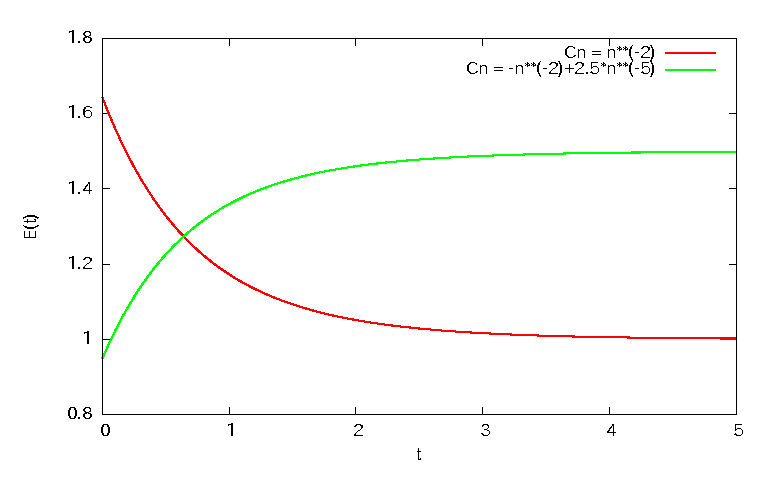
\includegraphics[width = 7cm]{./EPS/neq_fig1.eps}
    \figcaption{$\kappa = \overline{n} = 1$}
    \label{fig1}
  \end{minipage}
  \begin{minipage}{0.5\hsize}
    \centering
    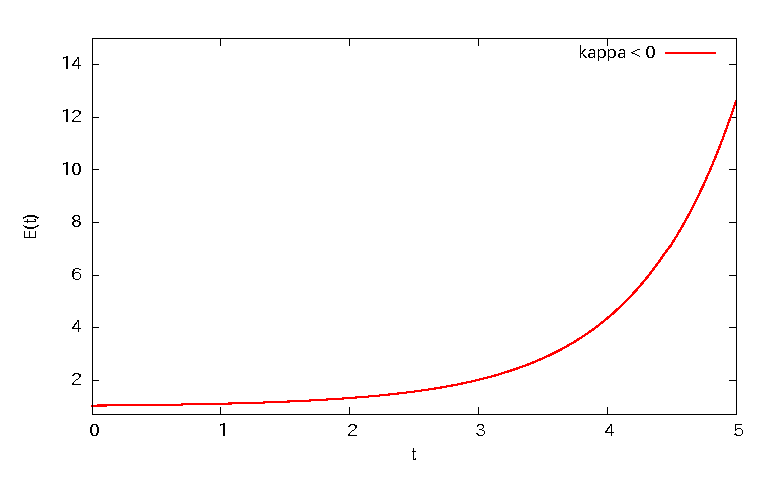
\includegraphics[width = 7cm]{./EPS/neq_fig2.eps}
    \figcaption{$\kappa$が負の場合}
    \label{fig2}
  \end{minipage}
\end{figure}
$E(0)$の情報は$C_n$に組み込まれており, さらに$C_n$の関数列の形に制限は収束すること以外には特にない. $E(0)$は$C_n$の汎関数だとも言える. つまり, $C_n$の与え方によって熱浴を通じてエネルギーが流出するか流入するかが決まる\footnote{系の初期温度が熱浴の温度$T$より大きければ流出するし,逆なら流入するのが普通. 非平衡状態では温度は定義できないので, 正確には流入・流出を支配しているのは温度ではなくエントロピーである.}. 汎関数は無限個の自由度を持つ関数なので$E(0)$は単なる系のエネルギーの初期値だけでなく,熱浴との相関具合などの自由度を含んでいる(かもしれない). 図1にエネルギーが緩和する様子を示した.今回は$C_n = \frac{1}{n^2}, -\frac{1}{n^2} + \frac{5}{2n^5}$の2つを計算. これは単に流入と流出を見たかったために選んできたものであり, $C_n$が収束するような関数列を選べば緩和は観測できるはず.

また, $\kappa$が負の場合, 振幅は減衰することなく増幅することを図2で確認している.
\section{線形応答理論}
\subsection{概要}
ある平衡系に$t = t_0$で何かしらの外場がかかったときの非平衡過程を見る理論. 摂動1次までの応答を見るので線形応答と呼ばれる.
\subsection{線形応答理論の基本概念}
平衡系のハミルトニアンを$H$, 外場$H_{\rm ex}(t)$としてFull Hamiltonian
\begin{eqnarray}
  H_{T} = H + H_{\rm ex}(t)
\end{eqnarray}
を考える. $H_{\rm ex}(t)$は$t< t_0$においてはゼロである. 平衡系の時間依存Schr\"odinger方程式:
\begin{eqnarray}
  i\partial_t\ket{\psi(t)} = H\ket{\psi(t)}
\end{eqnarray}
に対して外場を加えたSchr\"odinger方程式:
\begin{eqnarray}
  i\partial_t\ket{\Psi(t)} = \qty(H + H_{\rm ex}(t))\ket{\Psi(t)}
\end{eqnarray}
がある. $\ket{\Psi(t)}$は非平衡系の状態である. 平衡系の形式解が
\begin{eqnarray}
  \ket{\psi(t)} = e^{-iHt}\ket{\psi(0)}
\end{eqnarray}
であることから, ユニタリー演算子を用いて$\ket{\Psi(t)}$が
\begin{eqnarray}
  \ket{\Psi(t)} = e^{-iHt}U(t)\ket{\psi(0)}
\end{eqnarray}
と書けるものとする. これをSchr\"odinger方程式に代入すると
\begin{eqnarray}
  i\partial_t U(t) = e^{iHt}H_{\rm ex}(t)e^{-iHt}U(t) = H'_{\rm ex}(t)U(t)
\end{eqnarray}
という$U(t)$の時間発展方程式が得られる. ここで$H'_{\rm ex}(t)$は$H$による$H_{\rm ex}(t)$のHeisenberg描像になっている. 相互作用描像のときの議論と同様に
\begin{eqnarray}
  U(t) = 1 (t < t_0)
\end{eqnarray}
という条件を課すと
\begin{eqnarray}
  U(t) = 1 -i\int_{t_0}^{t}dt_1H'_{\rm ex}(t_1) + (-i)^2\int_{t_0}^{t}dt_1\int_{t_0}^{t_1}dt_2H'_{\rm ex}(t_1)H'_{\rm ex}(t_2) + \cdots
\end{eqnarray}
が得られる. 外場に対して1次のオーダーのみを扱うことにすると, 状態は
\begin{eqnarray}
  \ket{\Psi(t)} = e^{-iHt}\ket{\psi(0)} -ie^{-iHt}\int_{t_0}^{t}dt_1H'_{\rm ex}(t_1)\ket{\psi(0)}
\end{eqnarray}
となる. これを用いて任意の演算子$O(t)$(Schr\"odinger描像)の期待値は
\begin{eqnarray}
  \bra{\Psi(t)}O(t)\ket{\Psi(t)} &=& \bra{\psi(0)}\qty(1 + i\int_{t_0}^{t}dt_1H'_{\rm ex}(t_1))e^{iHt}O(t)e^{-iHt}\qty(1 - i\int_{t_0}^{t}dt_1H'_{\rm ex}(t_1))\ket{\psi(0)}\\
  &=& \bra{\psi(0)}O'(t)\ket{\psi(0)} + i\bra{\psi(0)}\int_{t_0}^{t}dt_1\qty[H'_{\rm ex}(t_1), O'(t)]\ket{\psi(0)} + \cdots
\end{eqnarray}
$O'(t) = e^{iHt}O(t)e^{-iHt}$であり, これまた$H$によるHeisenberg描像である. 外場が無い場合の期待値との差は$\ket{\psi_S(t)} = e^{-iH(t-t_0)}\ket{\psi_H(t_0)}$を用いて
\begin{eqnarray}
  \nonumber  \delta\bra{\Psi(t)}O(t)\ket{\Psi(t)} &=& \bra{\Psi(t)}O(t)\ket{\Psi(t)} - \bra{\psi(t)}O(t)\ket{\psi(t)}\\
  \nonumber  &=& \bra{\Psi(t)}O(t)\ket{\Psi(t)} - \bra{\psi(0)}e^{iHt}O(t)e^{-iHt}\ket{\psi(0)}\\
  \nonumber  &=& \bra{\Psi(t)}O(t)\ket{\Psi(t)} - \bra{\psi(0)}O'(t)\ket{\psi(0)}\\
  &=& i\bra{\psi(0)}\int_{t_0}^{t}dt_1\qty[H'_{\rm ex}(t_1), O'(t)]\ket{\psi(0)}\label{linear-zero}
\end{eqnarray}
外場が弱いと仮定して一次のオーダーまでその寄与を見ようというのが線形応答理論(linear response theory, 久保理論). 上式は描像がごちゃまぜになっているように見えるがSchr\"odinger描像とHeisenberg描像は
\begin{eqnarray}
  \ket{\psi(0)}_S = \ket{\psi(0)}_H
\end{eqnarray}
という関係にあるのであえてラベル付けをしていない.
\subsection{有限温度系へ}
次に(\ref{linear-zero})を有限温度の期待値に拡張する. これは単純に期待値の取り方を変えれば良い:
\begin{eqnarray}
  \delta\ev{O(t)} = \frac{\sum_j e^{\beta H_j}\delta\ev{O(t)}{i}}{\sum_j e^{\beta H_j}} = \frac{\Tr[\rho \delta O(t)]}{\Tr[\rho]} = i\int_{t_0}^{t}dt_1 \Tr\qty(\rho [H'_{\rm ex}(t_1), O'(t)])
\end{eqnarray}
ここで重要なことは(\ref{linear-zero})を見てもわかる通り, 非平衡系を記述するのに平衡系の情報しか用いていないことである. 逆を言えば取り扱いの難しい非平衡系の相互作用みたいな項は2次のオーダーから効いてくるということである\footnote{平衡系から大きくずれた非平衡系を取り扱うのに線形応答理論は不適切である. 尤も, そのような非平衡系の取り扱いはまだ明確に確立されていない. 量子マスター方程式は線形応答を超える枠組みとして期待されている.}. 線形応答は非平衡系のとても簡単な取り扱いの方法になっている.
\subsection{簡単な例}
$t = t_0$での外場の影響を
\begin{eqnarray}
  H_{\rm ex}(t) = \int d\bm{x} J(\bm{x}, t)\phi(\bm{x}, t)
\end{eqnarray}
のような形で考える. $J$はただのc-数で$\phi$は実スカラー場. 場の演算子$\phi(\bm{x}, t)$の熱平均を見ると
\begin{eqnarray}
  \delta\ev{\phi(\bm{x}, t)} &=& i\int_{t_0}^{t}dt_1 \Tr\qty(\rho\int d\bm{x}_1 \qty[J(\bm{x}_1, t_1)\phi'(\bm{x}_1, t_1), \phi'(\bm{x}, t)])\\
  &=& -i\int_{t_0}^{t}dt_1\int d\bm{x}_1J(\bm{x}_1, t_1)\Tr\qty(\rho\qty[\phi(\bm{x}, t), \phi'(\bm{x}_1, t_1)])\label{linear-temp}
\end{eqnarray}
ここでトレース部分はグリーン関数(2点相関関数)の定義になっている. 密度行列が規格化されていると仮定すると温度グリーン関数は
\begin{eqnarray}
  iD(\bm{x}, t; \bm{x}_1, t_1) =\ev{T\qty[\phi'(\bm{x}, t)\phi'(\bm{x}_1, t_1)]} = \Tr\qty[\rho T\qty(\phi(\bm{x}, t)\phi(\bm{x}_1, t_1))]
\end{eqnarray}
であり, 遅延グリーン関数を
\begin{eqnarray}
  iD_R(\bm{x}, t; \bm{x}_1, t_1) = \ev{[\phi'(\bm{x}, t), \phi'(\bm{x}_1, t_1)]}\theta(t-t_1) = \Tr\qty(\rho[\phi'(\bm{x}, t), \phi'(\bm{x}_1, t_1)])\theta(t-t_1)
\end{eqnarray}
と定義すれば(\ref{linear-temp})はこれを用いて
\begin{eqnarray}
  \delta\ev{\phi(\bm{x}, t)} &=& -\int_{-\infty}^\infty dt_1\int d\bm{x} D_R(\bm{x}, t; \bm{x}_1, t_1)J(\bm{x}_1, t_1)\\
  &=& -\int d^4xD_R(\bm{x}, t; \bm{x}_1, t_1)J(\bm{x}_1, t_1)
\end{eqnarray}
とまとめることができる. 時間$t$をまとめて4元ベクトルにしてしまっているが, 遅延グリーン関数の$\theta$関数で$t$が負のところは消えるので問題はない.

さて, これを今度は運動量表示に持っていく. 外場を加えているものの時間は平衡系のハミルトニアン$H$で発展しているので, 空間の一様性は保たれていると考える\footnote{もちろんこれは線形部分までしか考えていないから. }. $D_R, J$それぞれをフーリエ変換すると
\begin{eqnarray}
  D_R(\bm{x}, t; \bm{x}_1, t_1) &=& \int\frac{d^4p}{(2\pi)^4} e^{-ip(x-x_1)}D_R(\bm{p}, p_0)\\
  J(\bm{x}_1, t_1) &=& \int\frac{d^4p'}{(2\pi)^4}e^{-ip'x_1}J(\bm{p}', p'_0)
\end{eqnarray}
これを代入すると
\begin{eqnarray}
  \delta\ev{\phi(\bm{x}, t)} &=& -\int \frac{d^4p}{(2\pi)^4} e^{-ipx}J(\bm{p}, p_0)D_R(\bm{p}, p_0)\\
  \delta\ev{\phi(\bm{p}, p_0)} &=& -J(\bm{p}, p_0)D_R(\bm{p}, p_0)
\end{eqnarray}
というとても簡単な形に落ち着く. 結論としては, 外場の影響による熱平均の変化は運動量空間において外場のSource$J$と遅延グリーン関数$D_R$\footnote{これも当然, 外場のないときの遅延グリーン関数である. }を掛けたものになる.
\chapter{Wigner関数}
\section{Winger表示}
\subsection{定義}
Wigner関数の定義は以下の通り:
\begin{eqnarray}
  f_W(q, p, t) = \frac{1}{2\pi\hbar}\int_{-\infty}^{\infty} ds \bra{q-\frac{s}{2}}\ket{\psi(t)}\bra{\psi(t)}\ket{q+\frac{s}{2}}e^{ips/\hbar}\label{wigner1}
\end{eqnarray}
もしくは
\begin{eqnarray}
  f_W(q, p, t) = \int_{-\infty}^{\infty} d\overline{q}_{12} \bra{q_1}\ket{\psi(t)}\bra{\psi(t)}\ket{q_2}e^{-ip\overline{q}_{12}/\hbar}\label{wigner2}
\end{eqnarray}
とすることもできる. ここでは$q_{12} = (q_1 + q_2)/2$, $\overline{q}_{12} = q_1 - q_2$である.
\begin{comment}
  以下では(\ref{wigner})の流儀を採用することにする.
\end{comment}
\subsection{任意の演算子に対するWigner表示}
任意の演算子$\hat{A}$に対するWigner表示は
\begin{eqnarray}
  A_W(q_{12}, p) = \int_{-\infty}^{\infty} d\overline{q}_{12} \bra{q_1}\hat{A}\ket{q_2}e^{-ip\overline{q}_{12}/\hbar}\label{wigner_op}
\end{eqnarray}
である. ここで
\begin{eqnarray}
  \bra{q_1}\hat{A}\ket{q_2} = \frac{1}{2\pi}\int dp A_W(q_{12}, p)e^{-ip\overline{q}_{12}}\label{wigner_formula}
\end{eqnarray}
が成立している.
\section{Wigner分布関数の時間発展}
$f_W(q, p, t)$の時間発展方程式を導く. その準備として2つの演算子同士の積($\hat{A}\hat{B}$)のWigner変換がどのように計算できるかを考える. 
\subsection{$(\hat{A}\hat{B})_W$の計算}
今回は式(\ref{wigner1})の流儀を採用する:
\begin{eqnarray}
  (\hat{A}\hat{B})_W &=& \int_{-\infty}^{\infty}ds \bra{q-\frac{s}{2}}\hat{A}\hat{B}\ket{q+\frac{s}{2}}e^{ips/\hbar}
  = \int_{-\infty}^{\infty}\int_{-\infty}^{\infty}ds dq' \mel**{q-\frac{s}{2}}{\hat{A}}{q'}\mel**{q'}{\hat{B}}{q+\frac{s}{2}}e^{ips/\hbar}\label{wigner_start}
\end{eqnarray}
ここで式(\ref{wigner_formula})を用いて変形する:
\begin{eqnarray}
  \frac{1}{(2\pi\hbar)^2}\int ds dq' dp' dp'' e^{ips/\hbar}e^{-ip'\qty(q-q'-\frac{s}{2})/\hbar} e^{-ip''\qty(q'-q-\frac{s}{2})/\hbar}A_W\pqty{\frac{q+q'}{2} - \frac{s}{4}, p'}B_W\qty(\frac{q+q'}{2} + \frac{s}{4}, p'')
\end{eqnarray}
expの肩の変数に着目して$A_W, B_W$の変数を変形する:
\begin{eqnarray}
  \nonumber\frac{1}{(2\pi\hbar)^2}\int ds dq' dp' dp'' &&e^{ips/\hbar}e^{-ip'\qty(q-q'-\frac{s}{2})/\hbar} e^{-ip''\qty(q'-q-\frac{s}{2})/\hbar}\\
  && \times A_W\qty(q + \frac{1}{2}\pqty{q'-q-\frac{s}{2}}, p')B_W\qty(q - \frac{1}{2}\pqty{q-q'-\frac{s}{2}}, p'')
\end{eqnarray}
これを並進演算子を用いて
\begin{eqnarray}
  \nonumber\frac{1}{(2\pi\hbar)^2}\int ds dq' dp' dp'' &&e^{ips/\hbar}e^{-ip'\qty(q-q'-\frac{s}{2})/\hbar}e^{-ip''\qty(q'-q-\frac{s}{2})/\hbar}\\
  &&\times\qty(e^{\frac{1}{2}\pqty{q'-q-\frac{s}{2}}\partial_q}A_W\qty(q, p'))\qty(e^{-\frac{1}{2}\pqty{q-q'-\frac{s}{2}}\partial_q}B_W\qty(q, p''))
\end{eqnarray}
と変形. さらに並進変換$e^{a\partial_q}e^{pq} = e^{p(q+a)}$を用いて
\begin{eqnarray}
  \nonumber\frac{1}{(2\pi\hbar)^2}\int&& ds dq' dp' dp'' e^{ips/\hbar}\\
  &&\times\qty(A_W\qty(q, p')e^{\frac{i\hbar}{2}\overleftarrow{\partial}_q\overrightarrow{\partial}_{p''}}e^{-ip''\qty(q'-q-\frac{s}{2})/\hbar})\qty(e^{-ip'\qty(q-q'-\frac{s}{2})/\hbar}e^{-\frac{i\hbar}{2}\overleftarrow{\partial}_{p'}\overrightarrow{\partial}_{q}}B_W\qty(q, p''))
\end{eqnarray}
とする. ここで$\overleftarrow{\partial}, \overrightarrow{\partial}$はそれぞれ左側, 右側に作用する演算子である. 次に$q'$の積分を計算する:
\begin{eqnarray}
  \nonumber\frac{1}{2\pi\hbar}\int&& ds dp' dp'' e^{ips/\hbar}\\
  &&\times\qty(A_W\qty(q, p')e^{\frac{i\hbar}{2}\overleftarrow{\partial}_q\overrightarrow{\partial}_{p''}}e^{i(p'-p'')q/\hbar}\delta(p''-p')e^{-\frac{i}{2}(p''+p')s/\hbar}e^{-\frac{i\hbar}{2}\overleftarrow{\partial}_{p'}\overrightarrow{\partial}_{q}}B_W\qty(q, p''))
\end{eqnarray}
$p''$で積分:
\begin{eqnarray}
  &&\frac{1}{2\pi\hbar}\int ds dp' e^{ips/\hbar}\qty(A_W\qty(q, p')e^{\frac{i\hbar}{2}\overleftarrow{\partial}_q\overrightarrow{\partial}_{p'}}e^{-ip's/\hbar}e^{-\frac{i\hbar}{2}\overleftarrow{\partial}_{p'}\overrightarrow{\partial}_{q}}B_W\qty(q, p'))\\
  &=& \frac{1}{2\pi\hbar}\int ds dp' \qty(A_W\qty(q, p')e^{\frac{i\hbar}{2}\overleftarrow{\partial}_q\overrightarrow{\partial}_{p'}}e^{i(p-p')s/\hbar}e^{-\frac{i\hbar}{2}\overleftarrow{\partial}_{p'}\overrightarrow{\partial}_{q}}B_W\qty(q, p'))
\end{eqnarray}
$s$で積分:
\begin{eqnarray}
  \int dp' \qty(A_W\qty(q, p')e^{\frac{i\hbar}{2}\overleftarrow{\partial}_q\overrightarrow{\partial}_{p'}}\delta(p-p')e^{-\frac{i\hbar}{2}\overleftarrow{\partial}_{p'}\overrightarrow{\partial}_{q}}B_W\qty(q, p'))
\end{eqnarray}
最後に$p'$で積分:
\begin{eqnarray}
  \qty(A_W\qty(q, p)e^{\frac{i\hbar}{2}\overleftarrow{\partial}_q\overrightarrow{\partial}_{p}}e^{-\frac{i\hbar}{2}\overleftarrow{\partial}_{p}\overrightarrow{\partial}_{q}}B_W\qty(q, p))
\end{eqnarray}
つまり, $e^{\frac{i\hbar}{2}\qty(\overleftarrow{\partial}_q\overrightarrow{\partial}_{p}-\overleftarrow{\partial}_{p}\overrightarrow{\partial}_{q})} = e^{\frac{i\hbar}{2}\Lambda}$とおくと,
\begin{eqnarray}
  (\hat{A}\hat{B})_W = A_W(q, p)e^{\frac{i\hbar}{2}\Lambda}B_W(q, p)\label{wigner_end}
\end{eqnarray}
\subsection{$f_W(q, p, t)$の時間発展}
以上の結果を基に$f_W(q, p, t)$の時間発展方程式を導く. Schr\"odinger方程式
\begin{eqnarray}
  i\hbar\partial_t\ket{\psi(t)} = \hat{H}\ket{\psi(t)}
\end{eqnarray}
を用いて, 式(\ref{wigner2})の時間微分は以下のようにまとめられる:
\begin{eqnarray}
  i\hbar\partial_tf_W(q, p, t) &=& \int_{-\infty}^{\infty} d\overline{q}_{12} \bra{q_1}\qty(i\hbar\partial_t\ket{\psi(t)}\bra{\psi(t)})\ket{q_2}e^{-ip\overline{q}_{12}/\hbar}\\
  \nonumber  &=& \int_{-\infty}^{\infty} d\overline{q}_{12} \bra{q_1}(i\hbar\partial_t\ket{\psi(t)})\bra{\psi(t)}\ket{q_2}e^{-ip\overline{q}_{12}/\hbar}\\
  &&\hspace{0.5cm} + \int_{-\infty}^{\infty} d\overline{q}_{12} \bra{q_1}\ket{\psi(t)}(i\hbar\partial_t\bra{\psi(t)})\ket{q_2}e^{-ip\overline{q}_{12}/\hbar}\\
  &=& \int_{-\infty}^{\infty} d\overline{q}_{12} \mel**{q_1}{\comm{\hat{H}}{\ket{\psi(t)}\bra{\psi(t)}}}{q_2}e^{-ip\overline{q}_{12}/\hbar}\\
  &=& (\hat{H}\ket{\psi(t)}\bra{\psi(t)})_W - (\ket{\psi(t)}\bra{\psi(t)}\hat{H})_W\\
  &=& H_W(q, p)e^{\frac{i\hbar}{2}\Lambda}f_W(q, p, t) - f_W(q, p, t)e^{\frac{i\hbar}{2}\Lambda}H_W(q, p)\label{wigner-moyal}
\end{eqnarray}
\section{具体的な問題}
以上の定式化を具体的なモデルに落とし込み, 数値計算で相空間上の運動を見る.
\subsection{調和振動子系のWigner-Moyal方程式}
ハミルトニアンを
\begin{eqnarray}
  \hat{H} = \frac{\hat{p}^2}{2m} + \frac{1}{2}m\omega^2\hat{q}^2
\end{eqnarray}
とする. このハミルトニアンのWigner表示は
\begin{eqnarray}
  H_W(q, p) = \frac{p^2}{2m} + \frac{1}{2}m\omega^2q^2
\end{eqnarray}
である. これを(\ref{wigner-moyal})に代入:
\begin{eqnarray}
  i\hbar\partial_tf_W(q, p, t) = \qty(\frac{p^2}{2m} + \frac{1}{2}m\omega^2q^2)e^{\frac{i\hbar}{2}\Lambda}f_W(q, p, t) - f_W(q, p, t)e^{\frac{i\hbar}{2}\Lambda}\qty(\frac{p^2}{2m} + \frac{1}{2}m\omega^2q^2)
\end{eqnarray}
これを計算する. 面倒なので以下では$m = \omega = \hbar = 1$の単位系を採用.  
\begin{eqnarray}
  \partial_t f_W(q, p, t) = \qty(q\partial_p - p\partial_q)f_W(q, p, t)\label{wigner-moyal2}
\end{eqnarray}
のような偏微分方程式が導出される. これを数値的に解きたい.
\subsection{数値計算}
\subsubsection{差分化}
今回は簡単のため, 普通に差分化する. 差分化した方程式はMoyal方程式は
\begin{eqnarray}
  f(t_{n+1}) = k_1\qty[q_lf(p_{m+1}) - p_mf(q_{l+1})] + \qty[k_1(-q_l + p_m) + 1]f
\end{eqnarray}
となる. ここでいくつかの記号の省略ルールを示す:
\begin{itemize}
\item Wigner表示の添字$W$は省略
\item $f(q_l, p_m, t_n)$のように差分化しており, $q, p$の幅は$h_{qp}$, $t$の幅は$h_t$.
\item $f(q_l, p_m, t_n) \rightarrow f$, $f(q_{l+1}, p_m, t_n) \rightarrow f(q_{l+1})$などの表記を用いている.
\item $h_t/h_{qp} = k_1$.
\end{itemize}
これで数値計算が可能な形になった.
\subsubsection{問題点}
上の差分化は単なる前進差分なので${\cal O}(h_{qp}), {\cal O}(h_{t})$の誤差を生じる. これで計算すると, よほど細かく差分化しないとヤバいです. 誤差が累積して襲ってきます. せめて中央差分にしましょう. 
\subsubsection{初期条件}
%% 初期関数として
%% \begin{eqnarray}
%%   f_0 = \sqrt{\frac{5}{\pi}}e^{5(q+\frac{1}{2})^2}
%% \end{eqnarray}
%% を用意する(やる気なさ過ぎ?).
あるガウス波束$f_0$のWigner表示として
\begin{eqnarray}
  f_{0W} = \frac{1}{\pi}e^{-(q+4)^2 -p^2}\label{harmonic_wigner}
\end{eqnarray}
を用意する.$f_0$はこんなかんじ:
\begin{figure}[htbp]
  \centering
  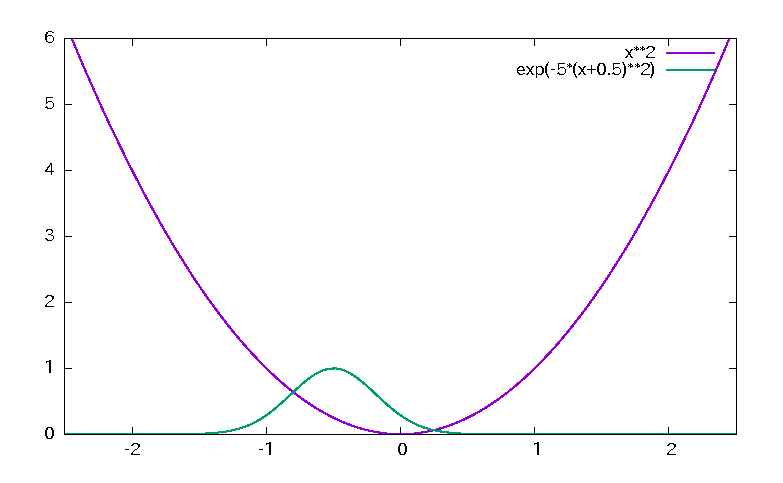
\includegraphics[width = 7cm]{./EPS/wave_packet.eps}
  \label{fig1}
\end{figure}
\\
この波束が調和型トラップによって振動する. 古典粒子が調和振動子トラップ内で振動するとき, 位相空間上の点は楕円を描くように動くはずでありWigner関数も同様の動きをするが, 相空間上では$q, p$方向の広がりがある. 
\begin{figure}[htbp]
  \begin{center}
    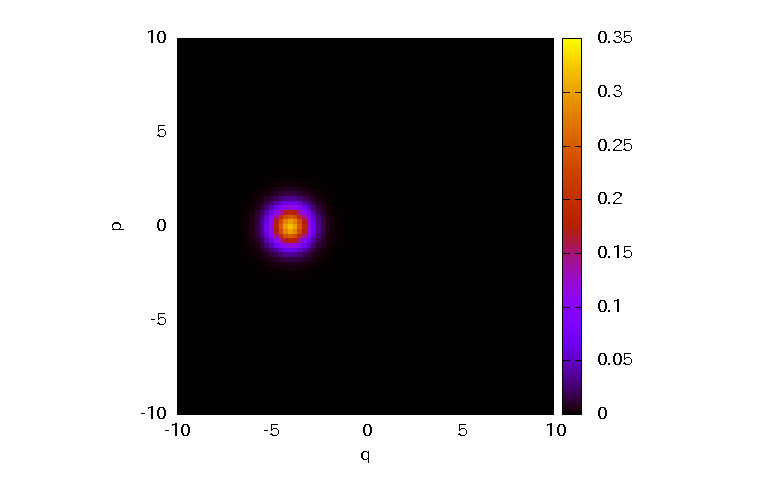
\includegraphics[width = 12cm]{./EPS/wigner_function.eps}
  \end{center}
  \label{fig2}
\end{figure}\\
こんなほんやりした玉みたいなのが位相空間上をぐるぐる回るはず. 
\newpage
\chapter{経路積分}
\section{量子力学の復習}
\subsection{自由粒子}
自由粒子を記述するSchr\"odinger方程式は
\begin{eqnarray}
  i\partial_t\ket{\psi(t)} = \frac{\hat{p}^2}{2m}\ket{\psi(t)}
\end{eqnarray}
これを$p$-表示に移すと簡単に解ける:
\begin{eqnarray}
  i\partial_t\bra{p}\ket{\psi(t)} &=& \bra{p}\frac{\hat{p}^2}{2m}\ket{\psi(t)} = \frac{p^2}{2m}\bra{p}\ket{\psi(t)}\\
  \therefore \bra{p}\ket{\psi(t)} &=& Ce^{-i\frac{\hat{p}^2}{2m}t}
\end{eqnarray}
これを運動量固有値$p$でパラメトライズされたケットで表現すると
\begin{eqnarray}
  \ket{p, t}_S = \ket{p}e^{-i\frac{\hat{p}^2}{2m}t}
\end{eqnarray}
ということ.もちろん$_S\bra{p', t}\ket{p, t}_S = \delta(p-p')$. 一般解はこの線型結合で書ける:
\begin{eqnarray}
  \ket{\Psi, t} = \int dp f(p)\ket{p}e^{-i\frac{\hat{p}^2}{2m}t}
\end{eqnarray}
これは規格化条件$\bra{\Psi, t}\ket{\Psi, t} = 1$を満たしているものとする. ここで, $t = 0$で$x = 0$に局在している波束を用意する:
\begin{eqnarray}
  \bra{x}\ket{\psi} = \frac{1}{(\pi\alpha)^{\frac{1}{4}}}e^{-\frac{1}{2\alpha}x^2}\label{FreeWavePacket}
\end{eqnarray}
これの$p$-表示は完全系を挿入することで求まる:
\begin{eqnarray}
  \bra{p}\ket{\psi} = \int dx\bra{p}\ket{x}\bra{x}\ket{\psi} = \qty(\frac{\alpha}{\pi})^{\frac{1}{4}}e^{-\frac{\alpha}{2}p^2}
\end{eqnarray}
\\

\fbox{問1} $\bra{x}\ket{p} = \frac{1}{\sqrt{2\pi}}e^{ipx}$であることを示せ. また, この操作がFourier変換と等価であることを確認せよ.\\

ここで$\Delta t$だけ時間発展させると
\begin{eqnarray}
  \bra{p}e^{-iH\Delta t}\ket{\psi} = \qty(\frac{\alpha}{\pi})^{\frac{1}{4}}e^{-\frac{\alpha}{2}p^2}e^{-i\frac{\hat{p}^2}{2m}\Delta t}
\end{eqnarray}
である. \\

\fbox{問2} $i\partial_t\ket{\psi} = \hat{H}\ket{\psi}$の形式解が$e^{-i\hat{H}t}\ket{\psi}$であることを確かめよ.\\

これを$x$-表示に移すと
\begin{eqnarray}
  \bra{x}\ket{\psi} = \qty(\frac{\alpha}{\pi})^{\frac{1}{4}}\sqrt{\frac{1}{\alpha + i\frac{\Delta t}{m}}}e^{-\frac{1}{\alpha + i\frac{\Delta t}{m}}x^2}\label{DevelopedFreeWavePacket}
\end{eqnarray}
となる. 自由粒子の波束の幅は時間発展と共に広がっていくことがわかる.
\subsection{Green関数}
以上のような「様々な初期波束を置いてみて, 時間発展に従って波動関数がどのように変化するのか」を考える問題ではGreen関数(伝搬関数, propagator)を計算しておくと便利.
\begin{eqnarray}
  \bra{x}\ket{\psi(t)} = \bra{x}e^{-iH(t-t_0)}\ket{\psi(t_0)} &=& \int dx'\bra{x}e^{-iH(t-t_0)}\ket{x'}\bra{x'}\ket{\psi(t_0)}\\
  &=& \int dx' G(x, t;x', t_0)\bra{x'}\ket{\psi(t_0)}
\end{eqnarray}
Green関数$G(x, t;x', t_0)$は, 時刻 $t_0$ に場所 $x_0$ にいた粒子が時刻$t$ に場所 $x$ に移動している確率振幅密度のようなもの. このGreen関数が分かりさえすれば波束を掛けて積分することで時間発展を追うことができる. このGreen関数を計算する方法としてよく用いられるのが経路積分である.

Green関数の数学的な定義などについては別途勉強しましょう.
\section{経路積分の基礎}
\subsection{経路積分の導出}
伝搬関数は初期状態を$(q_i, t_i)$, 終状態を$(q_f, t_f)$とすると
\begin{eqnarray}
  K(q_f, t_f;q_i, t_i) \equiv \bra{q_f, t_f}e^{-i\hat{H}(t_f-t_i)}\ket{q_i, t_i}
\end{eqnarray}
と定義できる\footnote{以降伝搬関数は$K$と書く. これをFeynman核(Feynman kernel)と呼ぶ. $t>0$を約束すればGreen関数とFeynman核は同じもの. }. $\ket{q, t}$は時刻$t$で粒子が座標$q$に局在している$\hat{q}$の固有状態である. 自由粒子などの簡単なモデルであれば伝搬関数の計算もそんなに大変ではないが, もっと複雑なモデルではそう簡単に求まらない. これをうまく計算するために経路積分(Path Integral)を導出する.

まず時間を微小区間$\delta t$に分割する:
\begin{eqnarray}
  e^{-i\hat{H}(t_f-t_i)} = \prod_{I=1}^Ne^{-i\hat{H}\delta t},\hspace{0.5cm} \delta t = \frac{t_f - t_i}{N}
\end{eqnarray}
時間を$N+1$分割したことになる. $\hat{q}$が$\hat{p}$より右側にあることを仮定し, 各分割点に位置演算子$\hat{q}(t_i + I\delta t)$の固有状態$\ket{q_I}$の完全系
\begin{eqnarray}
  \int dq_I \ket{q_I}\bra{q_I} = 1
\end{eqnarray}
を挟むと伝搬関数は以下のように書き直せる:
\begin{eqnarray}
  \nonumber  K(q_f, t_f;q_i, t_i) =\int dq_{N-1}dq_{N-2}\cdots dq_{I}\cdots dq_2dq_1\bra{q_f}e^{-i\hat{H}\delta t}\ket{q_{N-1}}\bra{q_{N-1}}e^{-i\hat{H}\delta t}\ket{q_{N-2}}\bra{q_{N-2}}\cdots\\
  \cdots\bra{q_{I+1}}e^{-i\hat{H}\delta t}\ket{q_{I}}\cdots\bra{q_2}e^{-i\hat{H}\delta t}\ket{q_1}\bra{q_1}e^{-i\hat{H}\delta t}\ket{q_i}
\end{eqnarray}
以下では$\bra{q_{I+1}}e^{-i\hat{H}\delta t}\ket{q_{I}}$を計算することを考える. これに運動量演算子$\hat{p}(t_i + I\delta t)$の固有状態$\ket{p_I}$の完全系
\begin{eqnarray}
  \int dp_I \ket{p_I}\bra{p_I} = 1
\end{eqnarray}
を挿入する:
\begin{eqnarray}
  \bra{q_{I+1}}e^{-i\hat{H}\delta t}\ket{q_{I}} &=& \int dp_I\bra{q_{I+1}}\ket{p_I}\bra{p_I}e^{-i\hat{H}\delta t}\ket{q_{I}}\\
  &=&\int dp_I\bra{q_{I+1}}\ket{p_I}e^{-iH(q_I, p_I)\delta t}\bra{p_I}\ket{q_{I}}
\end{eqnarray}\\

\fbox{問3} $\hat{H}$に演算子$\hat{q}, \hat{p}$が含まれていることから, $\bra{p_I}e^{-i\hat{H}\delta t}\ket{q_{I}}$のハットハミルトニアンが$c$-数の$H(q_I, p_I)$に化けることを示せ.\\

$\bra{q}\ket{p}$は平面波になることから
\begin{eqnarray}
  \bra{q_{I+1}}e^{-i\hat{H}\delta t}\ket{q_{I}} &=& \frac{1}{2\pi}\int dp_Ie^{i\qty(p_I\frac{q_{I+1}-q_I}{\delta t}-iH(q_I, p_I)){\delta t}}
\end{eqnarray}
$\delta t \rightarrow 0$の極限では$\cfrac{q_{I+1}-q_I}{\delta t}\rightarrow \cfrac{dq}{dt}$であることから
\begin{eqnarray}
  K(q_f, t_f;q_i, t_i) &=& \int {\cal D}p{\cal D}qe^{i\int_{t_i}^{t_f}dt\qty(p\frac{dq}{dt} - H)}\\
  {\cal D}p{\cal D}q &=& \prod_{I=0}^{N}\frac{{\cal D}p{\cal D}q}{2\pi}
\end{eqnarray}\\

\fbox{問4} expの肩が(和ではなく)積分になることを確認せよ.\\

$N$はいずれ$\infty$になるので, 無限回の積分を行わなくてはいけない。この積分は $q(t_i) = q_i, q(t_f) = q_f$ となるような境界条件をつけて行うとする.

$H = \frac{p^2}{2m} + V(q)$の場合について考える:
\begin{eqnarray}
  K(q_f, t_f;q_i, t_i) &=& \int {\cal D}p{\cal D}qe^{i\int_{t_i}^{t_f}dt\qty(p\frac{dq}{dt} - \frac{p^2}{2m} - V(q))} = \int {\cal D}p{\cal D}qe^{i\int_{t_i}^{t_f}dt\qty(-\frac{(p-m\dot{q})^2}{2m} + \frac{\dot{q}^2}{2m} - V(q))}
\end{eqnarray}
これで$p$について積分が可能. $q$の積分は$V(q)$の具体系が与えられて初めて計算が可能になる. $p$の積分を実行し, その解が${\cal N}$だったとすると
\begin{eqnarray}
  K(q_f, t_f;q_i, t_i) = {\cal N}\int {\cal D}qe^{i\int_{t_i}^{t_f}dt\qty(\frac{\dot{q}^2}{2m} - V(q))}\label{FeynmanPropagator}
\end{eqnarray}
$\exp$の肩に作用(action)$S[q(t)] = \int_{t_i}^{t_f}dt\qty(\frac{\dot{q}^2}{2m} - V(q))$に虚数単位を掛けて積分すれば伝搬関数が求まることがわかる. これが経路積分である.

作用が(プランク定数より)十分大きい場合$\exp(iS)$は極値の近傍を除いて激しく振動して積分に効いてこないことが期待される. この極値のみを取り出してきたものを「古典極限」と呼ぶ. 作用がプランク定数と同程度のオーダーを持つ場合, 極値近傍以外にも積分に効いてくる可能性があり, これが量子効果として取り入れられることになる.\\

\fbox{問5} 無次元化をしない場合, 経路積分の被積分関数は$\exp\qty(iS/\hbar)$と書ける. $S$がプランク定数$\hbar$より十分大きい時, $S$の極値以外の積分が値に効いてこない理由を考えよ. 

\subsection{自由粒子 : 経路積分を使わない方法}
自由粒子($V(q) = 0$)の場合は経路積分を使わなくても伝搬関数がすぐに求まる. まず$p$-表示で確率振幅を書き下す:
\begin{eqnarray}
  \bra{p_f}e^{-i\frac{\hat{p}^2}{2m}(t_f - t_i)}\ket{p_i} = e^{-i\frac{p_f^2}{2m}(t_f - t_i)}\delta(p_f - p_i)
\end{eqnarray}
これを$x$-表示に移す:
\begin{eqnarray}
  K(x_f, t_f;x_i, t_i) = \bra{x_f}e^{-i\frac{\hat{p}^2}{2m}(t_f - t_i)}\ket{x_i} &=& \int dp\bra{x_f}\ket{p}\bra{p}e^{-i\frac{\hat{p}^2}{2m}(t_f - t_i)}\ket{x_i}\\
  &=&\sqrt{\frac{m}{2\pi i(t_f-t_i)}}e^{-i\frac{m}{2(t_f - t_i)}(x_f - x_i)^2}\label{FreePropagator}
\end{eqnarray}\\
\fbox{問6} (\ref{FreePropagator})(\ref{DevelopedFreeWavePacket})を用いて(\ref{FreeWavePacket})を再現せよ.

\subsection{自由粒子 : 経路積分の方法}
まずは伝搬関数(の被積分関数)を時間について離散化する($\dot{x} = \cfrac{x_{j+1} - x_j}{\delta t}$):
\begin{eqnarray}
  e^{-i\int dt\frac{m\dot(x)^2}{2}} \rightarrow \prod_{j=0}^Ne^{\frac{im}{2}\qty(\frac{x_{j+1} - x_j}{\delta t})\delta t}
\end{eqnarray}
ただし$x_0 = x_i, x_{N+1} = x_f$とする. これに$\int dx_1dx_2\cdots dx_N$をかけて積分すれば(\ref{FeynmanPropagator})が計算できたことになる. ここで公式
\begin{eqnarray}
  \int_{-\infty}^{\infty} dx e^{ia(x-x_1)^2 + ib(x-x_2)^2} = \sqrt{\frac{i\pi}{a+b}}e^{i\frac{ab}{a+b}(x_1-x_2)^2}\label{Gauss}
\end{eqnarray}
を用いる. \\

\fbox{問7} (\ref{Gauss})を証明せよ.\\

$x_1$に関する積分:
\begin{eqnarray}
  \int dx_1 e^{i\frac{m}{2\delta t}\qty((x_i - x_1)^2-(x_1 - x_2)^2)} = \sqrt{\frac{i\pi\delta t}{m}}e^{-i\frac{m}{4\delta t}(x_i - x_2)^2}
\end{eqnarray}
これより, $x_2$の積分は:
\begin{eqnarray}
  \int dx_2 e^{i\frac{m}{2\delta t}\qty(\frac{1}{2}(x_i - x_2)^2-(x_2 - x_3)^2)} = \sqrt{\frac{4i\pi\delta t}{3m}}e^{-i\frac{m}{6\delta t}(x_i - x_3)^2}
\end{eqnarray}
これを繰り返していくと$x_n$の積分因子として$\sqrt{\cfrac{i2n\pi\delta t}{(n+1)m}}$が現れることがわかる. 全積分が終わったとき
\begin{eqnarray}
  K(x_f, t_f;x_i, t_i) = \bra{x_f}e^{-i\frac{\hat{p}^2}{2m}(t_f - t_i)}\ket{x_i} = {\cal N}\qty(\sqrt{\frac{i2\pi\delta t}{m}})^N\sqrt{\frac{1}{N+1}}e^{i\frac{m}{2(N+1)\delta t}(x_f - x_i)^2}\label{Kernel}
\end{eqnarray}
${\cal N}$は$p$積分の結果出てくる因子で, 積分1回につき$\sqrt{\cfrac{m}{2\pi i\delta t}}$が出てくる. さらに$\delta t(N+1) = t_f - t_i$であることを用いると
\begin{eqnarray}
  K(x_f, t_f;x_i, t_i ) &=&\sqrt{\frac{m}{2\pi i(t_f-t_i)}}e^{-i\frac{m}{2(t_f - t_i)}(x_f - x_i)^2}
\end{eqnarray}
となり, (\ref{FreePropagator})と一致している.\\

\fbox{問8} $p$成分の積分を計算せよ.\\

\fbox{問9} 数学的帰納法を用いてFeynman kernelが(\ref{Kernel})のように計算できることを示せ.\\

経路積分を使わない方法に比べてかなり面倒ですが, モデルがもっと複雑になると有り難みが出てきます. 
\section{数値計算の準備及び経路積分のイメージ}
直感的理解へ向けて経路積分について数値計算を行う.
\subsection{基底波動関数と伝搬関数}
伝搬関数を束縛状態の固有関数$\ket{n}$で展開:
\begin{eqnarray}
  G(x, t; x_0, t_0=0) \equiv \bra{x}e^{-i\hat{H}(t-t_0)}\ket{x_0} = \sum_n\bra{x}\ket{n}\bra{n}e^{-i\hat{H}t}\ket{x_0} = \sum_n\psi_n(x)\psi_n^*(x_0)e^{-iE_nt}
\end{eqnarray}
ここで$t = -i\tau$として$\tau\rightarrow\infty$を考えると, 高い励起状態は指数関数的に減衰していくことがわかる. これより伝搬関数と基底波動関数の関係
\begin{eqnarray}
  &&G(x, t= 0 -i\tau; x_0, t_0=0) \rightarrow \psi_0(x)\psi_0^*(x_0)e^{E_0\tau}\\
  &\therefore&|\psi_0(x)|^2 \rightarrow e^{-E_0\tau}G(x, t= 0 -i\tau; x_0=x, t_0=0)\label{GroundGreen}
\end{eqnarray}
が明らかになる. 第二式は始点と終点が同じになっていることに注意. Green関数から基底波動関数の情報を抜き出すためには, 虚時間を導入し時間発展を行えば良い. これを虚時間発展法と呼ぶ.
\subsection{作用とラグランジアン}
ラグランジアンを虚時間で記述すると, ハミルトニアンに化ける:
\begin{eqnarray}
  &&L\qty(x, \frac{dx}{dt}) = \frac{m}{2}\qty(\frac{dx}{dt})^2 - V(x)\\
  &\rightarrow& L\qty(x, \frac{dx}{-id\tau}) = -\frac{m}{2}\qty(\frac{dx}{d\tau})^2 - V(x) = -H\qty(x, \frac{dx}{d\tau})
\end{eqnarray}
これにより作用がラグランジアンの積分からハミルトニアンの積分に書き換えられる:
\begin{eqnarray}
  S[x(t)] &=& \int_{t_0=0}^{t}dtL(x, t) = i\int_{\tau_0=0}^{\tau}d\tau H(x,\tau)\label{prob10_1}\\
  G(x, -i\tau; x_0, 0) &=& \qty(\frac{1}{2\pi})^{N+1}\int dx_1 dx_2\cdots dx_N e^{-\int_0^{\tau} H(\tau)}\label{prob10_2}
\end{eqnarray}\\

\fbox{問10} (\ref{prob10_1})(\ref{prob10_2})を確かめよ. \\

\subsection{作用積分の簡略化}
前述のハミルトニアンの積分を差分化で書き直し, 数値計算に持ち込めるようにする:
\begin{eqnarray}
  \int H(\tau) &\simeq& \sum_j\epsilon E_j = \epsilon W(\{x_j\})\\
  W(\{x_j\}) &\equiv& \sum_j\qty[\frac{m}{2}\qty(\frac{x_{j} - x_{j-1}}{\epsilon})^2 + V\qty(\frac{x_{j} + x_{j-1}}{2})]
\end{eqnarray}
規格化を考慮したうえで(\ref{GroundGreen})に代入する:
\begin{eqnarray}
  |\psi_0(x)|^2 &=& \lim_{\tau\rightarrow\infty}\frac{G(x, t=-i\tau;x_0=x, t_0=0)}{\int dx G(x, t=-i\tau;x_0=x, t_0=0)}\\
  &=&\frac{1}{Z}\lim_{\tau\rightarrow\infty}\int dx_1 dx_2\cdots dx_N e^{-\epsilon W(x, x_1,..., x_N)}\label{PsiW}\\
  Z &=& \lim_{\tau\rightarrow\infty}\int dx dx_1 dx_2\cdots dx_N e^{-\epsilon W}
\end{eqnarray}
$W$はエネルギー線績分になっている. また$W(x, x_1,..., x_N)$は始点と終点を$x$に固定している.
\subsection{経路とは}
(\ref{prob10_2})の$\exp$の肩においてハミルトニアンを時間軸に沿って積分している. また$S[x(t)] = i\int_{\tau_0=0}^{\tau}d\tau H(x, \tau)$から作用は$x(t)$の経路によって決定される. つまり, 「取りうるすべての$x(t)$の経路についてエネルギー(ハミルトニアン)を足しあげていく」ことが経路積分の具体的なイメージである. エネルギーが大きい経路が効いてこない理由は(\ref{prob10_2})から直感的にわかる. 
\subsection{経路の取り方}
$|\psi_0(x)|^2$を求めたい訳だが, 数値計算の上では離散化するので$|\psi_0(x[1])|^2, |\psi_0(x[2])|^2, |\psi_0(x[3])|^2 ... |\psi_0(x[N-1])|^2$を求めることになる. 本来なら$G(x[1], -i\tau; x[1], 0), G(x[2], -i\tau; x[2], 0), G(x[3], -i\tau; x[3], 0), ... G(x[N-1], -i\tau; x[N-1], 0)$について別々の初期設定で計算する必要がある.これを別々に計算すると計算コストが非常に高くなる.$x_j$は時間で差分化, $x[j]$は空間で差分化していることに注意.

具体的な計算においては(\ref{PsiW})を各$x[1],x[2] ...$について計算すればよいのだが
\begin{eqnarray}
  |\psi_0(x[1])|^2 &=&\frac{1}{Z}\lim_{\tau\rightarrow\infty}\int dx_1 dx_2\cdots dx_N e^{-\epsilon W(x[1], x_1, x_2, ...)}\\
  |\psi_0(x[2])|^2 &=&\frac{1}{Z}\lim_{\tau\rightarrow\infty}\int dx_1 dx_2\cdots dx_N e^{-\epsilon W(x[2], x_1, x_2, ...)}\\
  \nonumber  &&\vdots
\end{eqnarray}
における$W(x[1], x_1, x_2, ...)$と$W(x[2], x_1, x_2, ...)$は始点(終点)が異なるので, それぞれ別々に計算を実行しなければならない. これが計算コストの肥大化の原因である.
\subsection{処方箋}
この問題に関する処方箋はRubinの本\footnote{Rubin H. Landau, {\it Computational Physics} (1997) pp. 313-317}にあるのでこれを参考勉強するのがいいと思います. が, 翻訳があまり良くないのかそもそも原文の内容が丁寧でないためか, 理解するのはなかなか難しいと思います. 理解のための重要なポイントは
\begin{itemize}
\item[1.] $x_0$が始点(終点)の経路における$x_i$を$x'_i$にフリップしたときに$x_0$からの作用積分が $x_i$からの作用積分と同じ値であることを利用して$|\psi(x'_i)|^2$を求めることが経路積分の計算と等価であること
\item[2.] 作用を計算して確率分布に計上することと, フリップする確率をBoltzmann分布で与えてその経路(格子点)に乗った粒子をそのまま足し上げることがだいたい等価であること
\end{itemize}
の2点にあると思います. この2つがMonte Carlo法・Metropolis法による数値計算を正当化しています.

是非一緒にお勉強しましょう. 
%% \subsection{計算のテクニック}
%% この問題を解消するために(\ref{PsiW})を以下のように変形する:
%% \begin{eqnarray}
%%   |\psi_0(x)|^2  &=&\frac{1}{Z}\lim_{\tau\rightarrow\infty}\int dx_0 dx_1 dx_2\cdots dx_N \delta(x - x_0)e^{-\epsilon W(x_0, x_1,..., x_N)}
%% \end{eqnarray}
%% これで始点(終点)を$x_0$に固定したことになる. 例えば$\psi(x[1]), \psi(x[2]), \psi(x[3])\cdots$を計算したければ
%% \begin{eqnarray}
%%   |\psi_0(x[1])|^2  &=&\frac{1}{Z}\lim_{\tau\rightarrow\infty}\int dx_0 dx_1 dx_2\cdots dx_N \delta(x[1] - x_0)e^{-\epsilon W(x_0, x_1,..., x_N)}\\
%%   |\psi_0(x[2])|^2  &=&\frac{1}{Z}\lim_{\tau\rightarrow\infty}\int dx_0 dx_1 dx_2\cdots dx_N \delta(x[2] - x_0)e^{-\epsilon W(x_0, x_1,..., x_N)}\\
%%   |\psi_0(x[3])|^2  &=&\frac{1}{Z}\lim_{\tau\rightarrow\infty}\int dx_0 dx_1 dx_2\cdots dx_N \delta(x[3] - x_0)e^{-\epsilon W(x_0, x_1,..., x_N)}\\
%% \nonumber  &&\vdots
%% \end{eqnarray}
%% を計算すればよい. ここで重要なのは「被積分関数はデルタ関数を除いてどれも同じ」ことである.つまり, $x_0$を始点に置いたすべての$(x_0, x_1, ..., x_N)$についてエネルギー線績分を計算した後に$x[1], x[2], x[3], ...$のそれぞれについてのみ値をピックアップすればよい.
%% \subsubsection{いやだから...}
%% 結局デルタ関数で$x_0$が$x[1]$やら$x[2]$やらに変えられるわけだから, やはり別々に$W(x[1], x_1, x_2, ...)$と$W(x[2], x_1, x_2, ...)$を計算しなければならないのでは?と思うでしょう.

%% この問題を巧く解決する方法があります\footnote{Rubin H. Landau, {\it Computational Physics} (1997) pp. 313-317}.

\newpage
\chapter{Ising模型}
\section{Ising模型と熱統計力学の基礎}
強磁性体を記述するモデルのひとつ.
\subsection{ハミルトニアン}
ハミルトニアンを
\begin{eqnarray}
  H = -J\sum_{\ev{i, j}}s_i\cdot s_j
\end{eqnarray}
とする. $\ev{i, j}$は隣接サイト間のみの和を表す. $J$は相互作用定数. $s$はスピン. スピンはアップ($s = 1$)とダウン($s = -1$)の2種類. 非常に単純なスピン系モデルでありながら相転移の記述が可能である. 1・2次元系については厳密解が求められている.

外部磁場を考慮したモデルもある:
\begin{eqnarray}
  H = -J\sum_{\ev{i, j}}s_i\cdot s_j -h\sum_i s_i\label{Ising2}
\end{eqnarray}

\subsection{平衡状態}
系の平衡状態はHelmholtzエネルギー
\begin{eqnarray}
  F = U -TS
\end{eqnarray}
が最小になるように決まる. 低温 ($T \ll U/S$)ならば内部エネルギー $U = \ev{H}$ がleading であり, これを最小化するようにスピンの向きが揃う. これを強磁性体と呼ぶ. 一方で高温ならばエントロピーの項が優勢なのでエントロピーが最大になるようにスピンの向きがバラバラになる. これを常磁性体と呼ぶ.

\subsection{相転移}
Gibbs自由エネルギーの1回微分が不連続変化をするときこれを第一種相転移と呼び, Gibbs自由エネルギーの2回微分については第二種相転移と呼ぶ. 第一種は体積, エントロピーとか. 
\begin{eqnarray}
  \qty(\frac{\partial G}{\partial p})_T = V, \hspace{1cm} \qty(\frac{\partial G}{\partial T})_p = -S
\end{eqnarray}
第二種は比熱など.
\begin{eqnarray}
  \frac{\partial^2 G}{\partial T^2} = -\frac{\partial S}{\partial T} = -\frac{C_P}{T}
\end{eqnarray}
有限温度1次元Ising模型は相転移を起こさないが, 2次元系はその限りではない.

\section{Ising模型の厳密解}
\subsection{1次元Ising模型 : 平均場近似}
まずは厳密解の前にIsing模型を平均場近似で解析してみる. 多体系で相互作用を平均場として理解することは非常に重要なので, 手法として知っておく必要がある.

平均場近似ではまず任意のサイトのスピンに着目し, その周囲のスピンからの影響を時間や空間によらない平均値で置き換える. スピンを
\begin{eqnarray}
  s_i = \ev{s} + \delta s_i
\end{eqnarray}
置くことにする. これを(\ref{Ising2})に代入:
\begin{eqnarray}
  H &=& -H_{\rm{eff}}\sum_{i=1}^N s_i + \frac{NzJ\ev{s}^2}{2}\\
  H_{\rm{eff}} &=&  h + zJ\ev{s}
\end{eqnarray}
ここで$\delta s$の2次は無視している. $N$はスピンの総数, $z$は最隣接サイト数(1次元なら2, 2次元なら4)である. 計算途中で
\begin{eqnarray}
  \sum_{\ev{i, j}}s_i = z\sum_i s_i, \hspace{0.5cm}\sum_{\ev{i, j}}1 = \frac{1}{2}zN
\end{eqnarray}
を用いている. これより分配関数は
\begin{eqnarray}
  Z &=& \exp\qty(-\beta H) = \exp\qty[-\beta\qty(-H_{\rm{eff}}\sum_{i=1}^N s_i + \frac{NzJ\ev{s}^2}{2})] = Z_0\qty(\prod_iZ_i) = Z_0(Z_i)^N\\
  Z_0 &=& \exp\qty(-\beta\frac{NzJ\ev{s}^2}{2}), \hspace{0.5cm}Z_i = \sum_{s_i = 1, -1}e^{\beta H_{\rm{eff}}s_i} = 2\cosh\qty(\beta H_{\rm{eff}})
\end{eqnarray}
全体の分配関数は
\begin{eqnarray}
  Z = \exp\qty(-\beta\frac{NzJ\ev{s}^2}{2})2^N\cosh^N\qty(\beta H_{\rm eff})
\end{eqnarray}
Helmholtzエネルギーは
\begin{eqnarray}
  F = \frac{NzJ}{2}\ev{s}^2 - Nk_BT\log\qty[2\cosh\qty(\beta H_{\rm eff})]
\end{eqnarray}
磁化は単位体積あたりのスピン数を$n$としたときに$M=n\ev{s}$であるが, 今回すべてのスピンは等価と考えているので$\ev{s_i}$を計算すれば十分である:
\begin{eqnarray}
  \ev{s_i} &=& \frac{1}{Z}\sum_{s_i}\cdots\sum_{s_i}\cdots s_ie^{-\beta H} = \frac{1}{Z_i}\sum_{s_i = -1, 1}s_ie^{\beta s_iH_{\rm eff}}\\
  &=& \tanh\qty(\beta H_{\rm eff})
\end{eqnarray}
これは自己無同着方程式である.
\subsection{1次元Ising模型 : 厳密解}
教科書を参考にしながら是非自分で手を動かして解いてみてください.
\subsection{2次元Ising模型}
2次元Ising模型の厳密解はOnsagerによって求められている:
\begin{eqnarray}
  \frac{U}{N} &=& -J\coth{2\beta J}\qty[1+\frac{2}{\pi}\kappa_1 K(\kappa)]\\
  \frac{C_H}{N} &=& k_B(\beta J\coth{2\beta J})^2\frac{2}{\pi}\qty[2K(\kappa)-2E(\kappa) - (1-\kappa_1)\qty(\frac{2}{\pi} + \kappa_1K(\kappa))]
\end{eqnarray}
$K(\kappa), E(\kappa)$は楕円積分:
\begin{eqnarray}
  K(\kappa) = \int_0^{\frac{\pi}{2}}\frac{d\theta}{\sqrt{1-\kappa^2\sin^2{\theta}}}\\
  E(\kappa) = \int_0^{\frac{\pi}{2}}d\theta \sqrt{1-\kappa^2\sin^2{\theta}}
\end{eqnarray}
導出は難しいので, これが数値計算と一致するかどうかを確かめたい. 

\section{数値計算}
\subsection{Monte Carlo法}
系はHelmholtzエネルギーを最小にするように平衡状態を決める(ゼロ温度の場合は内部エネルギーが最小).これを実現するためには, 任意のサイトの状態を変化させて内部エネルギーが小さくなるようにする操作を繰り返せば良い. 「任意のサイトを選ぶ」ために乱数を用いることになるが, 乱数を用いるアルゴリズムの総称がMonte Carlo法である.

単純に前述の通り内部エネルギーが最小な平衡状態はゼロ温度なので, 有限温度系に拡張するためには工夫が必要である. 
\subsection{Metropolis法}
系が平衡状態にあるとき, 内部エネルギーの分布を$P(E)$, エネルギー$E' \rightarrow E$遷移確率を$W(E, E')$とすると
\begin{eqnarray}
  W(E, E')P(E') = W(E', E)P(E)\label{equiliblium}
\end{eqnarray}
が成立している. $P(E')$の状態が$P(E)$の状態に遷移しようとする流れとその逆の流れが平衡状態にあるということである. 系のエネルギー分布がカノニカル分布になることを仮定すると, 
\begin{eqnarray}
  P(E) = \frac{e^{-\beta E}}{Z(\beta)}
\end{eqnarray}
であることがわかる. $Z(\beta)$は分配関数. これを(\ref{equiliblium})に代入すると以下の関係式を得る:
\begin{eqnarray}
  e^{-\beta(E-E')} = \frac{W(E, E')}{W(E', E)}\label{equiliblium2}
\end{eqnarray}
ここで, (\ref{equiliblium2})を満たすような$W(E, E')$を与える: 
\begin{eqnarray}
  W(E, E') =
  \begin{cases}
    1 & (E \leq E')\\
    e^{-\beta(E-E')} & (E > E')
  \end{cases}
\end{eqnarray}
これがMetropolis法である.

Isingモデルに置き換えると, スピンをフリップしたときにエネルギー的に安定ならばそのままにして, 不安定な場合も, ボルツマン因子に依る確率でフリップを許可する. これで有限温度系への拡張が可能になる. 
\newpage
\subsection{2次元Ising模型}
シミュレーション結果:
\begin{figure}[htbp]
  \begin{center}
    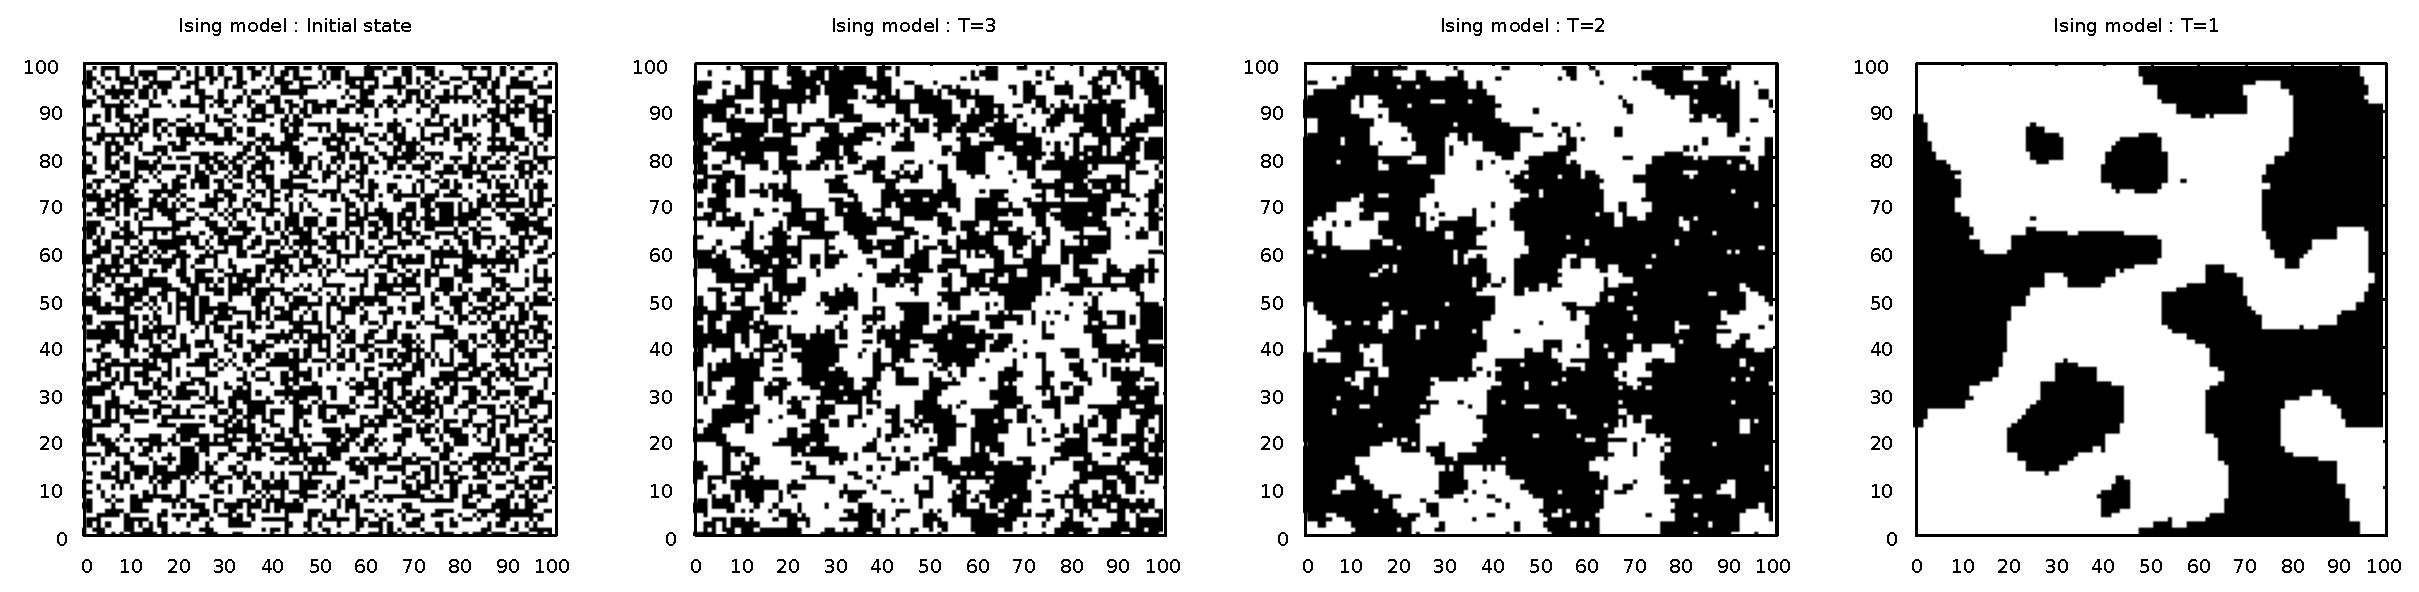
\includegraphics[width = 17cm]{./EPS/spin.eps}
  \end{center}
  \label{fig1}
\end{figure}\\
\begin{figure}[htbp]
  \begin{center}
    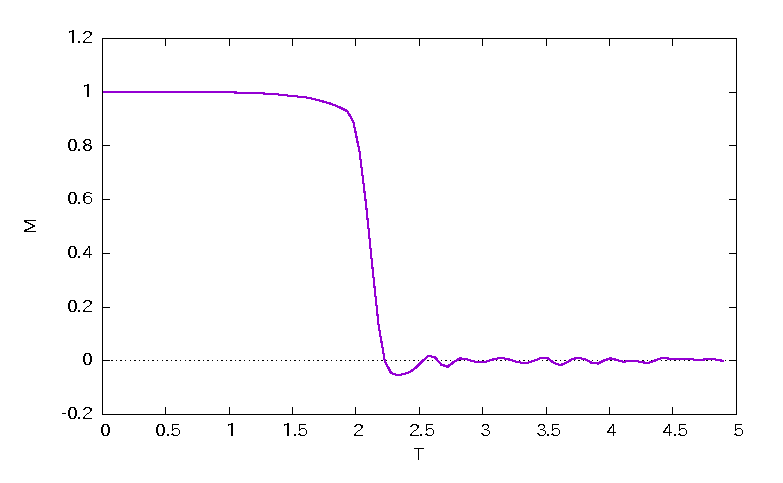
\includegraphics[width = 10cm]{./EPS/magnetization.eps}
  \end{center}
  \label{fig2}
\end{figure}\\
\begin{figure}[htbp]
  \begin{center}
    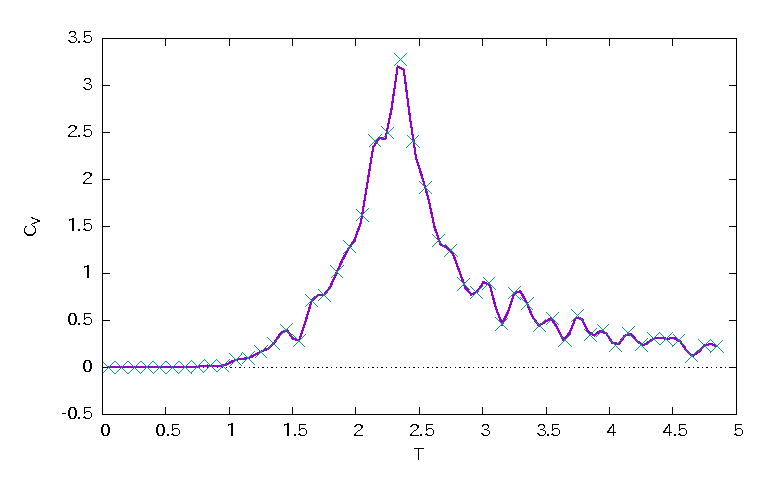
\includegraphics[width = 10cm]{./EPS/specificheat.eps}
  \end{center}
  \label{fig2}
\end{figure}\\

磁区の図は$N=100^2, J=1$, 磁化と比熱は$N=16^2, J=1$で計算した. 以上の図から
\begin{itemize}
\item 温度が下がるほどはっきりとした磁区が形成されること
\item 磁化・比熱は転移温度($T_C \simeq 2.26$)付近でdrasticに変化していること
\item 2次相転移が起こっている(であろう)こと
\end{itemize}
などがわかる.

\subsection{数値計算上の注意}
\subsubsection{乱数}
なるべく良い乱数を用いるようにしましょう. C言語のrand()はあまり良くありません. 単純な線形合同法では周期が短く大量の乱数を用いるシミュレーションには向きません. Mersenne twisterなどのアルゴリズムを用いましょう.
\subsubsection{ローカルな極小点}
ゼロ温度系ではあまり明確な磁区が生まれません. ただのMonte Carlo法ではローカルな極小点にハマるとそこから抜け出せないからです. Metropolis法を適応するとある程度解決しますが, やはり正の磁区と負の磁区に分かれるのでグローバルな磁化は熱力学極限とは異なる値を示します. 上の図の$T=1$もやはりローカルな極小点であり真の最小点であるスピンが全て揃った状態にはなりません. これを解決するために, 物理量の計算の際は$T=0$でスピンが全て揃った状態を用意しそこからMonte Carloシミュレーションを行っています. 焼きなまし法を用いるとどんな初期状態でもHelmholtzエネルギーが最小な状態を作れるかもしれません.
\begin{figure}[htbp]
  \begin{center}
    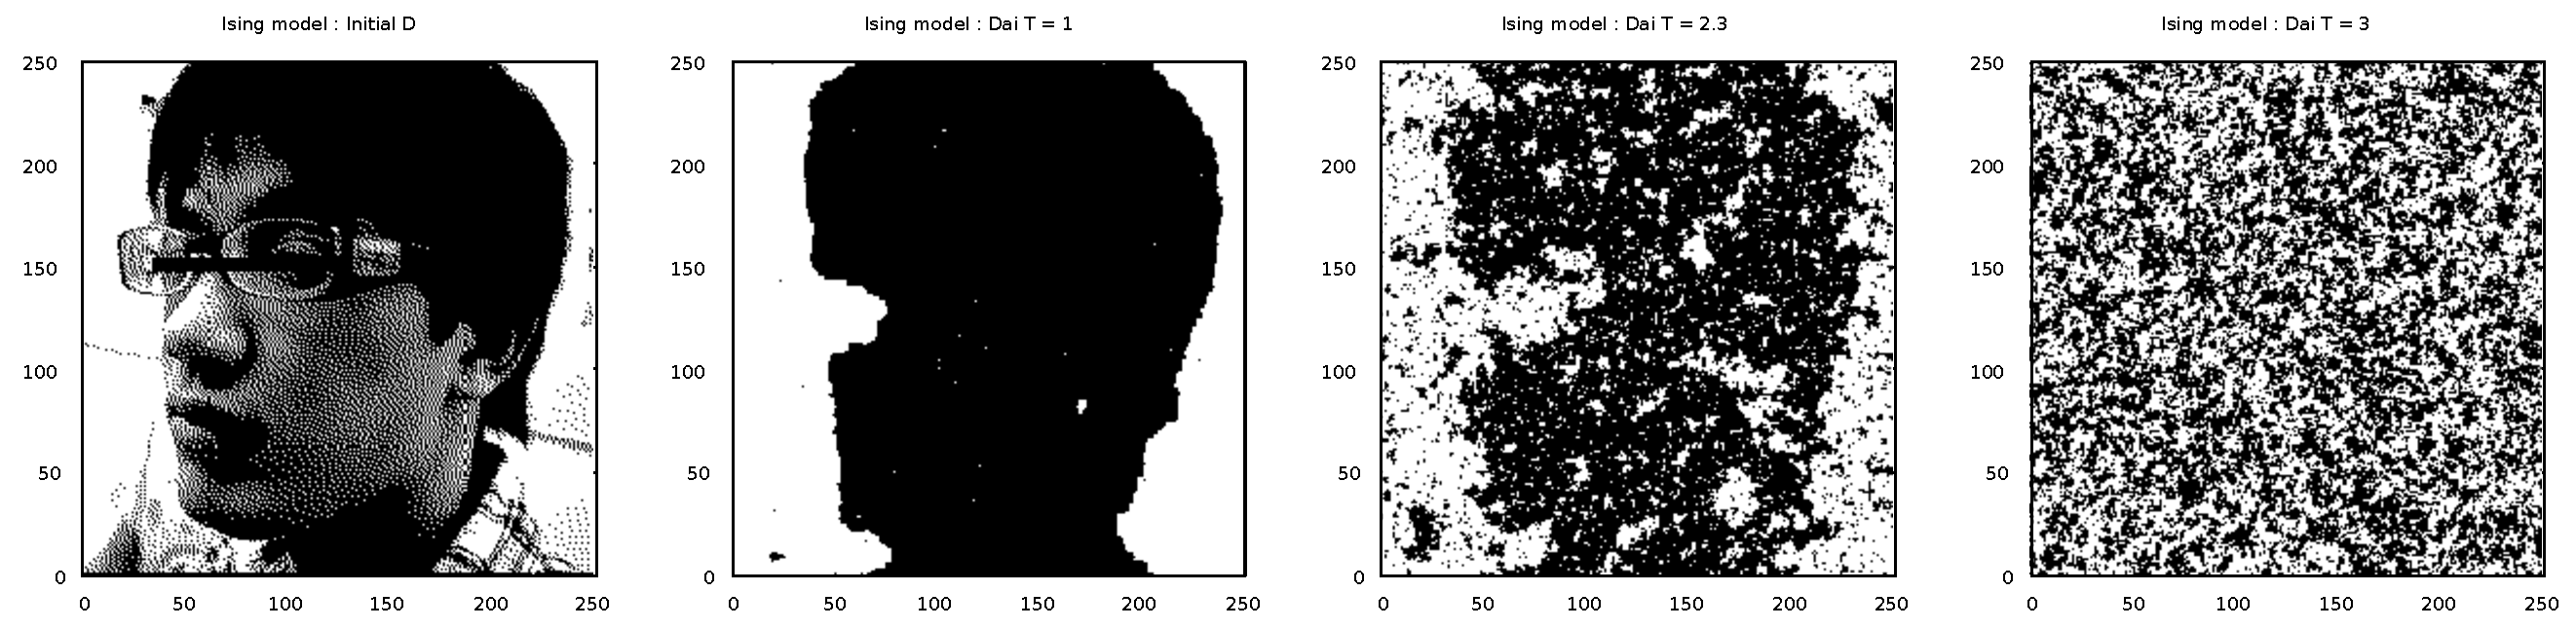
\includegraphics[width = 17cm]{./EPS/Dai.eps}
  \end{center}
  \label{Dai}
\end{figure}\\
ご覧の通り, Metropolis法だと磁化の形成は初期状態の選び方に強く依存します.

\newpage
\chapter{場の量子論}
\section{Wickの定理}
摂動計算において重要な役割を果たす. ただし, この定理が成立するのは\textbf{生成消滅演算子の代数を満たすものに限られる. }つまり, ゼロモード演算子はWickの定理を満たさない. 
\subsection{概要}
ざっくり言うと
\begin{screen}
  場の演算子の時間順序積(T積)はそれらの演算子から構成される全ての可能な正規積(N積)と伝搬関数の積の和で表される.
\end{screen}
伝搬関数(因果Green関数, Feynman propagator)は
\begin{eqnarray}
  \Delta_F(\bm{x}_1-\bm{x}_2, t_1-t_2) = -i\bra{0}{\rm T}\left[\phi(\bm{x}_1, t_1)\phi^\dagger(\bm{x}_2, t_2)\right]\ket{0}
\end{eqnarray}
で与えられるので, $\phi$の可能な組を全て足し上げればよい. 伝搬関数は$\phi^\dagger, \phi$の組で作られるので, $\phi\phi, \phi^\dagger\phi^\dagger$の組は考えなくても良い. 
N積は生成演算子を前に, 消滅演算子を後ろに持ってくる順序積:
\begin{eqnarray}
  :\phi_1\phi^\dagger_2\phi_3\phi^\dagger_4:\ = \phi^\dagger_2\phi^\dagger_4\phi_1\phi_3
\end{eqnarray}

大事なことは, \textbf{N積の真空期待値は必ずゼロになるということ}と, \textbf{演算子が時間に依存していないならば勝手にT積をつけてもよい}ということ. 期待値を計算するための面倒な交換関係計算があるとき, Wickが使えることがある. 基本的には伝搬関数が真空で作られているので有限温度では使えないが, 議論を有限温度期待値に拡張したBlock-de Dominicsの定理というのがある. 有限温度系におけるWickの定理とかも呼ばれる. 
\subsection{具体例}
\subsubsection{n=2の場合}
\begin{eqnarray}
  {\rm T}[\phi_1\phi_2] =\ :\phi_1\phi_2: + \bra{0}{\rm T}[\phi_1\phi_2]\ket{0}
\end{eqnarray}
\subsubsection{n=3の場合}
\begin{eqnarray}
  {\rm T}[\phi_1\phi_2\phi_3] =\ :\phi_1\phi_2\phi_3: + \bra{0}{\rm T}[\phi_1\phi_2]\ket{0}\phi_3 + \bra{0}{\rm T}[\phi_1\phi_3]\ket{0}\phi_2 + \bra{0}{\rm T}[\phi_2\phi_3]\ket{0}\phi_1 
\end{eqnarray}
\subsection{証明}
Fetterの章を参照のこと. 
\section{TFD形式による期待値計算}
$k$が連続自由度を持つ場合の期待値をTFDの力を借りて計算する.
\subsection{TFDのド基礎}
熱的真空は
\begin{eqnarray}
  \ket{0} &=& (1-f)\sum_mf^m\dket{m, m}\\
  \bra{0} &=& \sum_m\dbra{m, m}
\end{eqnarray}
で定義される. $f$はボルツマン因子. $f \neq e^{-\beta\omega}$のとき非平衡であるという. 熱的ブラ・ケットは双対ではない.
超演算子形式における$\dbra{I_R}\bullet\dket{\rho_R}$は熱的真空期待値$\ev{\bullet}{0}$に置き換えが可能\footnote{超演算子形式のチェック・チルダとTFDのノンチルダ・チルダは単射同型の関係にある. }. またBosonの熱的Bogoliubov変換の具体形は
\begin{eqnarray}
  b_{\bm{k}}^\dagger &=& \tilde{\xi_{\bm{k}}} + (1+n_{\bm{k}})\xi_{\bm{k}}^\dagger\\
  b_{\bm{k}} &=& \xi_{\bm{k}} + n_{\bm{k}}\tilde{\xi_{\bm{k}}}^\dagger
\end{eqnarray}
で与えられ, $\xi$演算子は熱的真空を消去する消滅演算子である:
\begin{eqnarray}
  \xi\ket{0} &=& \tilde{\xi}\ket{0} = 0\ ,\hspace{0.5cm} \bra{0}\xi^\dagger = \bra{0}\tilde{\xi}^\dagger = 0\\
  \comm{\xi}{\xi^\dagger} &=& \comm{\tilde{\xi_{\bm{k}}}}{\tilde{\xi_{\bm{k}'}}^\dagger} = \delta(\bm{k}-\bm{k}'), \hspace{0.5cm} \comm{\xi_{\bm{k}}}{\tilde{\xi_{\bm{k}'}}} = \comm{\xi_{\bm{k}}}{\tilde{\xi_{\bm{k}'}}^\dagger} = 0
\end{eqnarray}
この熱的真空, $\xi$演算子を用いて計算をする. 以下$x = (\bm{x}, t), y = (\bm{y}, s)$とする. 
\subsection{具体計算}
例として以下の計算をする:
\begin{eqnarray}
  \ev{R_3(x)R_3(y)} &\equiv& \bra{0}\frac{1}{(2\pi)^6}\int dk_1dk_2dk_3dk_4 b^\dagger_{k_1}b_{k_2}b^\dagger_{k_3}b_{k_4}e^{-i(k_1-k_2)x}e^{-i(k_3-k_4)y}e^{i(\omega_{k_1}-\omega_{k_2})t}e^{i(\omega_{k_3}-\omega_{k_4})s}\ket{0}\\
  \nonumber  &=& \frac{1}{(2\pi)^6}\int dk_1dk_2dk_3dk_4e^{-i(k_1-k_2)x}e^{-i(k_3-k_4)y}e^{i(\omega_{k_1}-\omega_{k_2})t}e^{i(\omega_{k_3}-\omega_{k_4})s}\\
  && \bra{0}\qty(\tilde{\xi_1} + (1+n_1)\xi_1^\dagger)\qty(\xi_2 + n_2\tilde{\xi_2}^\dagger)\qty(\tilde{\xi_3} + (1+n_3)\xi_3^\dagger)\qty(\xi_4 + n_4\tilde{\xi_4}^\dagger)\ket{0}
\end{eqnarray}
ここでは$\xi, n$の添字について$(k_1, k_2, k_3, k_4)\rightarrow(1, 2, 3, 4)$という置換をしている. 上式の熱的真空期待値を計算する:
\begin{eqnarray}
  &&\bra{0}\qty(\tilde{\xi_1} + (1+n_1)\xi_1^\dagger)\qty(\xi_2 + n_2\tilde{\xi_2}^\dagger)\qty(\tilde{\xi_3} + (1+n_3)\xi_3^\dagger)\qty(\xi_4 + n_4\tilde{\xi_4}^\dagger)\ket{0}\\
  =&&\bra{0}\tilde{\xi_1}\qty(\xi_2 + n_2\tilde{\xi_2}^\dagger)\qty(\tilde{\xi_3} + (1+n_3)\xi_3^\dagger)n_4\tilde{\xi_4}^\dagger\ket{0}\\
  =&&\bra{0}\qty(\tilde{\xi_1}\xi_2 + n_2\tilde{\xi_1}\tilde{\xi_2}^\dagger)\qty(n_4\tilde{\xi_3}\tilde{\xi_4}^\dagger + n_4(1+n_3)\xi_3^\dagger \tilde{\xi_4}^\dagger)\ket{0}\\
  =&&\bra{0}\qty(\tilde{\xi_1}\xi_2 + n_2\Bqty{\tilde{\xi_2}^\dagger\tilde{\xi_1} + \comm{\tilde{\xi_1}}{\tilde{\xi_2}^\dagger}})\qty(n_4\Bqty{\tilde{\xi_4}^\dagger\tilde{\xi_3} + \comm{\tilde{\xi_3}}{\tilde{\xi_4}^\dagger}} + n_4(1+n_3)\xi_3^\dagger \tilde{\xi_4}^\dagger)\ket{0}\\
  =&&\bra{0}\qty(\tilde{\xi_1}\xi_2 + n_2\delta(1-2))\qty(n_4\delta(3-4) + n_4(1+n_3)\xi_3^\dagger \tilde{\xi_4}^\dagger)\ket{0}\\
  \nonumber  = &&\bra{0}\qty(\tilde{\xi_1}\xi_2n_4\delta(3-4) + \tilde{\xi_1}\xi_2\xi_3^\dagger \tilde{\xi_4}^\dagger n_4(1+n_3) + n_2n_4\delta(1-2)\delta(3-4) + \xi_3^\dagger \tilde{\xi_4}^\dagger n_2n_4(1+n_3)\delta(1-2))\ket{0}\\
  \\
  = &&\bra{0}\qty(\tilde{\xi_1}\xi_2\xi_3^\dagger \tilde{\xi_4}^\dagger n_4(1+n_3) + n_2n_4\delta(1-2)\delta(3-4))\ket{0}\\
  = &&\bra{0}\Bqty{n_4(1+n_3)\delta(1-4)\delta(2-3) + n_2n_4\delta(1-2)\delta(3-4)}\ket{0}
\end{eqnarray}
よって
\begin{eqnarray}
  \nonumber  \ev{R_3(x)R_3(y)} &\equiv&\qty(\frac{1}{(2\pi)^3}\int dk n_k)^2 + \frac{1}{(2\pi)^6}\int dk_1dk_2 e^{-i(k_1-k_2)(x-y)}e^{i(\omega_{k_1}-\omega_{k_2})(t-s)}n_1(1+n_2)\label{expectation2}\\
\end{eqnarray}
\subsection{Block-de Dominicsの定理}
TFD形式だと計算が簡単になることがわかった\footnote{超演算子形式のままだとトレース演算になるのでなかなか面倒. }. ただ, 熱平均についてはBlock-de Dominicsの定理というWickの定理に対応するものがあるので, もっと簡単に計算できそうである. $b_1\sim b_6$まであるものを考えるが, $x, y$がcoupleするか否かは区別しないといけない\footnote{たとえば$1x-2x$がcoupleすると対応するデルタ関数$\delta(1-2)$が出てきて$e^{-i(k_1 - k_2)(x-y)}, e^{i(\omega_1 - \omega_2)(t-s)}$が消える.これは(\ref{expectation2})の右辺第一項にあたる項の起源. 一方で$x-y$のcross couplingがあるとexponentialの空間・時間成分が消えずに残る. これが(\ref{expectation2})の右辺第二項にあたる.}:
\begin{eqnarray}
  \ev{R_1(x)R_1^\dagger(y)} &\sim& \bra{0}b_{1x}^\dagger b^\dagger_{2x} b_{3x} b^\dagger_{4y} b_{5y} b_{6y} \ket{0} =\bra{0}{\rm T} \bqty{b_{1x}^\dagger b^\dagger_{2x} b_{3x} b^\dagger_{4y} b_{5y} b_{6y} }\ket{0}\\
  &=& 2\bra{0}{\rm T}\wick{321}{<1b_{1x}^\dagger <2b^\dagger_{2x} <3b_{3x} >3b^\dagger_{4y} >1b_{5y} >2b_{6y} }\ket{0} + 4\bra{0}{\rm T}\wick{321}{<1b_{1x}^\dagger <2b^\dagger_{2x} >1b_{3x} <3b^\dagger_{4y} >2b_{5y} >3b_{6y} }\ket{0}\\
  &=&2\ev{b^\dagger_{1x}b_{5y}}\ev{b^\dagger_{2x}b_{6y}}\ev{b_{3x}b^\dagger_{4y}} + 4\ev{b^\dagger_{1x}b_{3x}}\ev{b^\dagger_{2x}b_{5y}}\ev{b^\dagger_{4y}b_{6y}}\\
  \nonumber  &=& 2\delta(1-5)\delta(2-6)\delta(3-4)n_1n_2(1+n_3) + 4\delta(1-3)\delta(2-5)\delta(4-6)n_1n_2n_4\\
\end{eqnarray}
$\xi$演算子で真面目に計算しなくてもいける. 
\section{Gell-Mann-Lowの定理}
\subsection{断熱因子}
ハミルトニアンの摂動部が断熱因子を持っている場合を考える:
\begin{eqnarray}
  H = H_0 + e^{-\epsilon|t|}H_I
\end{eqnarray}
これは$t = 0$でfullの相互作用を取り入れた系になり, $t \rightarrow \pm\infty$で自由粒子になるようなハミルトニアンである. ここで, $t = t_0$かつ$t_0 \sim -\infty$で相互作用描像の状態が非摂動ハミルトニアンの固有状態になっている場合を考える\footnote{相互作用描像も自由粒子のハイゼンベルグ描像と一致するという近似できる. }:
\begin{eqnarray}
  H_0\ket{\Psi(t_0)}_I = E_0\ket{\Psi(t_0)}_I
\end{eqnarray}
さらに$t_0 \sim -\infty$であることから時間発展演算子を用いてハイゼンベルグ描像は
\begin{eqnarray}
  \ket{\Psi}_{\rm H} =  \ket{\Psi(0)}_I = U_\epsilon(0, t_0)\ket{\Psi(t_0)}_I= U_\epsilon(0, -\infty)\ket{\Psi(t_0)}_I\label{5eq1}
\end{eqnarray}
と書ける. これは, 相互作用系の状態が非摂動系の固有状態を用いて表現できたことを意味している.

あとは$\epsilon$について考える必要がある. そもそもこの系は2つの粒子の散乱実験をテーマにしたようなものである. 2つの粒子が$t = 0$で衝突することを考えるとき, 相互作用が効いてくるのは$t = 0$近傍のみであって, それ以外は自由粒子とほぼ同じ振る舞いをするだろうというアイデアから断熱因子は導入されている. 粒子を平面波的に記述するためにも$\epsilon\rightarrow 0$としたいが, この極限のもとで果たして(\ref{5eq1})は意味ある結果を与えるのだろうか?

これに答えるのがGell-Mann-Lowの定理である.\textbf{以降は基底状態に対する議論であることに注意.}
\subsection{概要}
Gell-Mann-Lowの定理が主張することは
\begin{eqnarray}
  \lim_{\epsilon\rightarrow0}\frac{U_\epsilon(0, -\infty)\ket{\phi_0(-\infty)}_I}{_I\bra{\phi_0(-\infty)}U_\epsilon(0, -\infty)\ket{\phi_0(-\infty)}_I} = \frac{\ket{\Psi_0}_H}{_I\expval{\phi_0(-\infty)|\Psi_0}_H}\label{gml}
\end{eqnarray}
が存在するなら固有状態$\ket{\Psi_0}_{\rm H}$はwell-definedであり, 固有値は
\begin{eqnarray}
  E-E_0 = \frac{_I\bra{\phi_0(-\infty)}H_I\ket{\Psi_0}_H}{_I\expval{\phi_0(-\infty)|\Psi_0}_H}
\end{eqnarray}
で与えられるということである. ここで添字の0は真空を意味している. また, $\ket{\phi_0(-\infty)}$は非摂動ハミルトニアンの固有状態になっているので解析的に求めることができる. あとは, (\ref{gml})が成立するかどうかが問題になる.

これが成立すればFree Hamiltonian $H_0$とFull Hamiltonian $H$をユニタリー演算子でつなぐことができる. つまり, Free Hamiltonianの固有状態$\ket{\Phi_0}$を求めたあとにユニタリー演算子$U(0, -\infty)$をAll orderで取り入れればFull Hamiltonianの固有状態が求まることになる. もちろんAll orderは無理なので摂動的に取り入れることになる. これが場の理論における摂動論である.

場の理論で物理量を摂動的に評価するときにはGreen関数を計算することが基本になるが, それを計算可能にするためのテクニックがWickの定理であり, そのWickの定理の証明にGell-Mann-Lowが用いられている. そういう意味でとっても重要. 
\subsection{証明}
Fetterの章を参照のこと.
\section{Bethe-Salpeter方程式}
Green関数の無限次数までの足し上げに関する処方, 特にLadder近似についての勉強をする. 一様系の議論が一般的. 有限サイズ系にも応用したいが...
\subsection{Bethe-Salpeterへの準備 : 1体Green関数}
まずは普通の1体Green関数(2点Green関数)のおはなし. Green関数の極がハミルトニアンのエネルギーを表していることを用いてエネルギーを求める. Green関数は
\begin{eqnarray}
  iG(x-x') = \ev{T[\varphi(x)\varphi^\dagger(x')]}{0}
\end{eqnarray}
で定義される. Fourier変換を
\begin{eqnarray}
  iG(x-x') = \frac{1}{(2\pi)^4}\int d^4k\;e^{ik(x-x')}G(k)
\end{eqnarray}
のように導入すると, Dyson方程式は
\begin{eqnarray}
  G(x_1-x_2) &=& G_0(x_1-x_2) + \int d^4y_1d^4y_2\;G_0(x_1-y_1)\Sigma^*(y_1-y_2)G(y_2-x_2)\\
  G(k) &=& G_0(k) + G_0(k)\Sigma^*(k)G(k)\\
  &=& G_0(k) + G(k)\Sigma^*(k)G_0(k)
\end{eqnarray}
整理すると
\begin{eqnarray}
  &&G^{-1}_0(k)G(k) = 1 + \Sigma^*(k)G(k)\\
  &&G(k)G^{-1}_0(k) = 1 + G(k)\Sigma^*(k)\\
  &\therefore& \qty(G^{-1}_0(k) - \Sigma^*(k))G(k) = G(k)\qty(G^{-1}_0(k) - \Sigma^*(k)) = 1
\end{eqnarray}
から, G(k)が極を持つとき
\begin{eqnarray}
  \det\qty[G^{-1}_0(k) - \Sigma^*(k)] = 0
\end{eqnarray}
を満たしている. これで$k_0$が$\bk$の関数として定まることになる.
\subsection{2体Green関数}
以下「物性研究者のための場の量子論」の表式に沿う. 2体Green関数
\begin{eqnarray}
  G_2(x_1, x_2, x_3, x_4) = \qty(-\frac{i}{\hbar})^2\ev{T\qty[\varphi(x_1)\varphi(x_2)\varphi^\dagger(x_3)\varphi^\dagger(x_4)]}{0}
\end{eqnarray}
を定義する. ここで$t_1 = t_2 = t, t_3 = t_4 = t'$とおくものとする. これは時刻$t'$に2個の粒子が$\bx_3, \bx_4$に存在したとき, 時刻$t$に2個の粒子が$\bx_1, \bx_2$に存在する確率振幅である. 1体問題のときと同様にFourier変換を導入する:
\begin{eqnarray}
  G_2(x_1, x_2, x_3, x_4) = \frac{1}{(2\pi)^8}\int d^4pd^4p'd^4kG_2(p, p';k)e^{i(\frac{2}{k}+p)x_1}e^{i(\frac{2}{k}-p)x_2}e^{-i(\frac{2}{k}+p')x_3}e^{-i(\frac{2}{k}-p')x_4}
\end{eqnarray}
このうち独立な空間変数は$x_1-x_2,\ x_3-x_4,\ x_1+x_2-x_3-x_4$の3つである. よくやる重心座標と相対座標による分解も行える:
\begin{eqnarray}
  &&(x_1+x_2)/2 = X,\hspace{1cm} x_1-x_2 = x\\
  &&(x_3+x_4)/2 = X',\hspace{1cm} x_3-x_4 = x'
\end{eqnarray}
\subsection{Bethe-Salpeter方程式}
ここで天下り的に, $G_2(p, p';k)$に対してBethe-Salpeter方程式を導入する:
\begin{eqnarray}
  G_2(p, p';k) = G_0(p, p';k) + \int d^4p''d^4p'''\;G_0(p, p';k)K(p'', p''';k)G_2(p, p';k)
\end{eqnarray}
右辺第二項の$G_0, G_2$は交換しても良い. 形からしてもDyson方程式で証明はできそう. 後でやる. ここで
\begin{eqnarray}
  G_0(p, p';k) \equiv G(k/2+p)G(k/2-p)\qty{\delta^4(p-p') - \delta^4(p-p')}
\end{eqnarray}
であり, $K$はproper self-energyに対応するとして話を進める. ここで$G_2(p, p';k)$を$p$行$p'$列の行列と考えて
\begin{eqnarray}
  G_2(k) &=& G_0(k) + G_0(k)K(k)G_2(k)\\
  &=& G_0(k) + G_2(k)K(k)G_0(k)  
\end{eqnarray}
と表現しておく. $G_0$は2体Green関数であることに注意. 先ほどのアナロジーから
\begin{eqnarray}
  \det\qty[G_0^{-1} - K(k)] = 0
\end{eqnarray}
で$G_2(k)$の極が与えられることは明らか.

%---------------------- comment -------------------------------
%---------------------- comment -------------------------------
\begin{comment}
  Bethe-Salpeter波動関数を
  \begin{eqnarray}
    \bra{0}T\qty[\varphi(x_1)\varphi(x_2)]\ket{\Phi_B} = \frac{1}{(2\pi)^{3/2}}e^{ikX}e^{-iE_BT/\hbar}\chi_k(x)
  \end{eqnarray}
  とおく. ただし$\Phi_B$は
  \begin{eqnarray}
    H\Phi_B = E_B\Phi_B
  \end{eqnarray}
  を満たす状態ベクトル. $\chi_k(x)$は内部座標$x$のみから決まる部分.

  次に必要なのはGreen関数と波動関数の関係, つまり$G_2$と$\chi_k(x)$の関係である. いま$t>t'$とすると,
  \begin{eqnarray}
    G_2(x_1, x_2, x_3, x_4) = \qty(-\frac{i}{\hbar})^2\ev{T[\varphi(x_1)\varphi(x_2)]T[\varphi^\dagger(x_3)\varphi^\dagger(x_4)]}{0}
  \end{eqnarray}
\end{comment}
%---------------------- comment -------------------------------
%---------------------- comment -------------------------------

\subsection{$K(k)$の構成}
$K(p, p';k)$をどのように構成するかを考える. まずはFeynman diagramを用いて形式的な方程式を書き下してみる.  
\section{ゼロモード演算子とBdGモードの成り立ち}
ゼロモード入門(中村)では各モード表現としてW行列を導入し, いろいろな対称性を議論している. これはゼロモードの完全系が時間発展する場合に必要とされるが, stationaryな議論をする場合はこれは必須ではない. 議論がややこしいので何をしようとしているのかがわかりづらいかもしれないが, 重要なのは
\begin{eqnarray}
  \qty[a_{\ell}, a^\d_{\ell'}] = \delta_{\ell\ell'}, \hspace{1cm} \qty[Q, P] = i
\end{eqnarray}
である. この一見当たり前に見える関係が, どのような仮定のもとで導出されているかを見る. これをしっかり理解できれば, 場の量子論が本質的に持つ自己無撞着性についての理解が深まると思う.
\subsection{場の理論の自己無撞着性}
ゼロモード入門には「$\xi$の決定に$\ket{0}$が必要・$\ket{0}$の決定に$\xi$が必要」というような文言があるが, これをもう少し詳しく見ると,
  
\\\\
0. 公理として$\psi$の同時刻CCR(正準交換関係)$\qty[\psi(x), \psi^\d(x')] = \delta(\bx - \bx')$がある. \\
1. $\ev{\psi}{0} = \xi + \varphi$を満たす真空$\ket{0}$を仮定. \\
2. ($\xi$を含む)Bogoliubov-de Gennes方程式の直交性から完全系を定義.\\
3. BdG完全系で展開される場の演算子が$\psi(\varphi)$のCCRを満たす.
  
\\\\
というシナリオを踏むことになる. そもそも「$\ket{0}$を決定する」とは「正しい準粒子描像を選択する」ことであり, 「準粒子描像」とは場の演算子がどのようなモード(今回であればBdGモード$a_\ell, a^\d_\ell, u_\ell, v_\ell$とゼロモード$Q, P, \xi, \eta$)で展開されるかを表すことば\footnote{と鳥居は思ってます. 割とナイーブな話なので, 山中先生に「違う!」とか言われても知りませんが. }.

あと「Bogoliubov-de Gennes完全系を定義」と書いていますが, 正確には「仮定」です. 完全系に先立つ真空$\ket{0}$が仮定なわけですから. 場の量子論では, 存在するかどうかもわからない$\ket{0}$を仮定して, その仮定の下で存在するかもわからない$\xi$を仮定し, さらにその仮定の下で存在するかもわからないBogoliubov-de Gennes完全系を仮定し...と繰り返していった結果, 最初の仮定である$\ket{0}$の選び方が実は正しかった!みたいなことをよくします. これからそれを見ていきます. 
\subsection{完全系の仮定}
前節で「完全系を定義」と書いたが, これは論理的に導出できるものではない. 「議論に矛盾がないように構成する」と言ったほうが正確. BdG完全系は
\begin{eqnarray}
  \sum_{\ell}\qty[y_{\ell}(\bx)y^\d_{\ell}(\bx') - z_{\ell}(\bx)z^\d_{\ell}(\bx')] + y_{0}(\bx)y^\d_{-1}(\bx') + y_{-1}(\bx)y^\d_{0}(\bx')  = \sigma_3\delta(\bx - \bx')\label{completeness2}
\end{eqnarray}
である. 
\begin{screen}
  \fbox{1}\ \ 正規直交性の関係
  \begin{eqnarray}
    \qty(y_{\ell}, y_{\ell'}) = \delta_{\ell\ell'}, \hspace{0.7cm}\qty(z_{\ell}, z_{\ell'}) = -\delta_{\ell\ell'}, \hspace{0.7cm}\qty(y_{0}, y_{-1}) = 1
  \end{eqnarray}
  を用いて場の演算子$\Phi = \qty(\varphi\ \ \varphi^\d)^t$を展開すると
  \begin{eqnarray}
    \sum_{\ell}\qty[A_\ell y_{\ell}(\bx) - B_\ell z_{\ell}(\bx)] + Cy_{0}(\bx) + Dy_{-1}(\bx)  =
    \begin{pmatrix}
      \varphi(x)\\
      \varphi^\dagger(x)
    \end{pmatrix}
  \end{eqnarray}
  となる. $A_\ell , B_\ell , C, D$はどうなるか?
\end{screen}
このとき, 山中研では$y_\ell(\bx) = \qty(u_\ell (\bx)\ \ v_\ell (\bx))^t$という表記がよく用いられる(そのとき$z_\ell(\bx)$はどうなる?).
\subsection{場の展開}
さて, 完全系によって場の演算子が展開できたので, 展開した場の演算子がCCRを満たすかどうかを確認したい. そのためには$A_\ell, B_\ell, C, D$各々の交換関係が必要である. 
\begin{screen}
  \fbox{2}\ \ $A_\ell, B_\ell, C, D$各々の交換関係を計算せよ(ゼロにならないのはどの組み合わせか?). \\
  また, $A_\ell, B_\ell, C, D$にはどのような演算子を割り当てるのが妥当か?
\end{screen}
ここまでくれば消滅演算子$a_\ell$と, 量子座標$Q, P$を用いた
\begin{eqnarray}
  \varphi(x) = \sum_\ell \qty[u_\ell(\bx) a_\ell(t) + v^*_\ell(\bx) a^\d_\ell(t)]  -iQ(t)\xi(\bx) + P(t)\eta(\bx)\label{expand-varphi}
\end{eqnarray}
のような展開になるのはわかるだろう\footnote{$Q$の前に虚数単位$i$をつけるのもちょっと考えればわかるはず}.
\begin{screen}
  \fbox{3}\ \ (\ref{expand-varphi})の交換関係を計算し, CCRになっていることを確認せよ. \\
  (完全性(\ref{completeness2})に戻せるか?)
\end{screen}
これで
\\\\
\textbf{CCR}$\rightarrow\ \ket{0}$を仮定$\rightarrow\ \xi$の存在を仮定$\rightarrow\ $Bogoliubov-de Gennes完全系を仮定$\rightarrow\ $場の演算子$\varphi$を展開するモードを仮定$\rightarrow\ $\textbf{CCR}
\\\\
ときれいに一周するので, つまるところ$\ket{0}, \xi$等すべての物理量が自己無撞着に定義できたことになる.
\subsection{なぜうまくいったか?}
あの完全系(\ref{completeness2})が恐らく一意的ものだとすると, 準粒子描像の選び方たるモードの定義も一意的になり, 議論の自由度がなくなりそうな気もしてくる. 「たまたまうまい$\ket{0}$を選んだら全てがうまくいってた」ところの「たまたま」の自由度はどこにあるのだろうか?

これは非摂動ハミルトニアン$H_u$にある. 非摂動/摂動ハミルトニアンの選び方は本来任意であるので, 異なる非摂動ハミルトニアンを定義すると異なる真空を選ぶことに対応する. 真空というのは, 相互作用描像の下で定義されるものであり, 相互作用描像は非摂動/摂動ハミルトニアンの選び方に依存するのである\footnote{ゼロモード入門にも「場の理論では$\ket{0}$を$H_u$の基底状態に取る」と書いてあります(ただし, それ以外の真空を選ぶことすらもできます). }. 基本的に, \textbf{理論の自由度は非摂動ハミルトニアンの選び方にかかっている}\footnote{いわゆる「繰り込み」も非摂動ハミルトニアンの取り方を変えてあげましょう, ということをやっている. }.

しかしご存知のように, うまくいったように見えてまだ問題は存在する. 
\subsection{なぜ問題(赤外発散)が発生するか}
今までの話からわかる通り, \textbf{非摂動ハミルトニアンの選び方が良くなかったのである}.
もっと正しい準粒子描像を選びましょう, ということ\footnote{場の理論の欠陥である紫外発散を質量の繰り込みで回避する, ということも, 山中研に言わせれば「理論の欠陥ではなく, 正しい準粒子描像を選んでない」ということになる. だいたいそういうやつは自由ハミルトニアンを非摂動ハミルトニアンに選んでしまっているようです. そりゃうまくいかないよね. }. その試みがInteracting ZeroMode Formulation(IZMF)である. 詳しくはゼロモード入門で.

\section{Bose系の有限温度Green関数}
一様有限温度Boson系における一般的なGreen関数についてまとめる.
\subsection{有限体積系におけるハミルトニアン}
Bose系の相互作用を考えないHeisenbergハミルトニアンは以下の通り:
\begin{eqnarray}
  H_{\rm H} = \int d\bx \psi_{\rm H}^\d(\bx)\qty(-\frac{\nabla^2}{2m} - \mu)\psi_{\rm H}(\bx)
\end{eqnarray}
$\psi(x)$を離散変数$k_n$でFourier級数展開した場合を考える. 体積$V$の有限系について:
\begin{eqnarray}
  \psi(\bx) = \frac{1}{\sqrt{V}}\sum_{n=-\infty}^{n=\infty}e^{i{\bk}_n\bx}a_{{\bk}_n}
\end{eqnarray}
ただし${\bk}_n = \frac{(2\pi)^3}{V}n$とする.これをハミルトニアンに代入すると
\begin{eqnarray}
  H = \sum_k \qty(\frac{k^2}{2m} -\mu)a_{\bk}^\d a_{\bk} = \sum_{\bk} \xi_{\bk}a_{\bk}^\d a_{\bk}
\end{eqnarray}
を得る($\xi_{\bk}$は秩序変数とは関係ない). デルタ関数が体積になることを用いている. Fullハミルトニアンが生成消滅演算子の2次なので, 真空はHeisenberg描像の$a_{\bk}$で張ることになる. 以後明示しない限り演算子は全てHeisenberg描像. 

ちなみに
\begin{eqnarray}
  \int dx\ \psi(x)e^{-ik_nx} &=& \frac{1}{\sqrt{L}}\sum_{n'}\int dx\ e^{-i(k_n-k_{n'})x}a_{k_{n'}}\\
  &=& \frac{1}{\sqrt{L}}\sum_{n'}L\delta_{nn'}a_{k_{n'}} = \sqrt{L}a_{k_n}\\
  \therefore a_{k_n} &=& \frac{1}{\sqrt{L}}\int dx\ \psi(x)e^{-ik_nx}  
\end{eqnarray}
このとき交換関係は
\begin{eqnarray}
  [a_{k_n}, a^\dagger_{k_{n'}}] = \frac{1}{L}\int dx dx'\ e^{-i(k_nx - k_{n'}x')}\left[\psi(x), \psi^\dagger(x')\right] = \frac{1}{L}\int dx \ e^{-i(k_n - k_{n'})x} = \delta_{nn'}
\end{eqnarray}
であり, これによって
\begin{eqnarray}
  \expval{a_{k_n}^\dagger a_{k_n}} = \frac{1}{e^{\beta\omega_{k_n}}-1} \equiv n_{k_n}
\end{eqnarray}
が保証される\footnote{付録B参照}. 連続へ拡張する場合は$[a_{\bk}, a^\d_{\bk'}] = \delta(\bk - \bk')$を守るように, 変換$a_{\bk_n}\rightarrow ca_{\bk}$の定数$c$を決めなければならない. 
\subsection{松原Green関数}
温度Green関数はGreen関数の虚時間形式であり, 実時間形式の有限温度Green関数とは別物. 紛らわしいのでここでは前者を松原Green関数と呼ぶ.

虚時間$\tau = it$を導入して先ほどの場の展開を用いると, 松原Green関数は以下のようにまとまる:
\begin{eqnarray}
  {\cal G}(\bm{r}, \bm{r}'; \tau, 0) &=& -\ev{T\psi(\bm{r}, \tau)\psi^\d(\bm{r}', 0)} = -\ev{\psi(\bm{r}, \tau)\psi^\d(\bm{r}', 0)}\\
  &=& -\frac{1}{V}\sum_{{\bk}_1, {\bk}_2}\ev{a_{{\bk}_1}(\tau)a^\d_{\bk_2}(0)}e^{i\bk_1\cdot\br}e^{-i\bk_2\cdot\br'}\\
  &=&-\frac{1}{V}\sum_{\bk}\ev{a_{\bk}a^\d_{\bk}}e^{-\xi_{\bk}\tau}e^{i\bk(\br - \br')}
\end{eqnarray}
計算を進めるために松原Green関数をFourier展開する:
\begin{eqnarray}
  {\cal G}(\bk, i\omega_n) &=& \int_0^\beta d\tau e^{i\omega_n\tau}\int d(\br-\br')e^{-i\bk\cdot(\br-\br')}{\cal G}(\br, \br';\tau, 0)
\end{eqnarray}
ここで, 一行目の$\tau$-積分の区間はどのように決まったのか, $\omega_n$が何者かを考えなければならない. そもそも熱力学量は
\begin{eqnarray}
  \ev{A(t)} &=& \Tr[\rho A(t)]/Z\\
  &=& \Tr[e^{-\beta H} A(t)e^{\beta H}e^{-\beta H}]/Z\\
  &=& \Tr[e^{i(iH\beta)} A(t)e^{-i(iH\beta)}e^{-\beta H}]/Z\\
  &=& \Tr[A(t+i\beta)e^{-\beta H}]/Z\\
  &=& \Tr[e^{-\beta H}A(t+i\beta)]/Z\\
  &=& \ev{A(t+i\beta)}
\end{eqnarray}
でわかるように, $i\beta$(虚時間なら$\beta$)周期性を持っている. これを久保-Martin-Schwinger(KMS)条件という. というわけで, ${\cal G}$は周期性を持ちFoureir級数展開の周波数に対応する. これを松原周波数という. 積分を実行すると
\begin{eqnarray}
  {\cal G}(\bk, i\omega_n) &=& -(1 + n_{\bk})\int_0^\beta d\tau \exp[(i\omega_n - \xi_{\bk})\tau]\\
  &=& \frac{1}{i\omega_n-\xi_{\bk}}
\end{eqnarray}
$\tau$-積分がちょうど$-(1+n_{\bk})^{-1}$に対応する.
\subsection{遅延Green関数とLehmann表示と解析接続}
ところで, 実時間形式のGreen関数はどんなものだったかというと,
\begin{eqnarray}
  iG(\bx, \bx';t, t') = \ev{T\qty[\psi(x)\psi^\d(x')]}
\end{eqnarray}
こういうのだった. しかしいざ計算しようとすると複素平面の上半分と下半分のどちらにも極が含まれているので扱いづらいという理由から, 極が片方にしかない遅延/先進Green関数を
\begin{eqnarray}
  iG^R(\bx, \bx';t, 0) = \ev{\qty[\psi(x), \psi^\d(x')]}\theta(t)
  iG^A(\bx, \bx';t, 0) = \ev{\qty[\psi(x), \psi^\d(x')]}\theta(-t)
\end{eqnarray}
のように定義して, これを元のGreen関数と結びつけて計算してやろうということをする. 例えば遅延Green関数は
\begin{eqnarray}
  G^R(k, \omega) &=& \int dte^{i\omega t}\int d(\bx-\bx')e^{-i\bk(\bx -\bx')}{\cal G}(\bx-\bx':t, 0)\\
  &=& -i\int dte^{i\omega t}\int d(\bx-\bx')e^{-i\bk(\bx -\bx')}\ev{\qty[\psi(x), \psi^\d(x')]}\theta(t)\\
  &=& -i\int dte^{i\omega t}\int d(\bx-\bx')e^{-i\bk(\bx -\bx')}\int d\bk'\ev{\qty[a_{\bk}(t), a^\d_{\bk}]}e^{i\bk'\cdot(\bx - \bx')}\theta(t)\\
  &=& -i\int dte^{i\omega t}\theta(t)\ev{\qty[a_{\bk}(t), a^\d_{\bk}]}\\
  &=& -i\int dte^{i\omega t}\theta(t)\qty(\ev{a_{\bk}(t)a^\d_{\bk}} - \ev{a^\d_{\bk}a_{\bk}(t)})\\
  &=& -i\int dte^{i\omega t}\theta(t)\sum_{nm}\qty(\ev{\rho a_{\bk}(t)\ket{m}\bra{m}a^\d_{\bk}}{n} - \ev{\rho a^\d_{\bk}\ket{m}\bra{m} a_{\bk}(t)}{n})/Z\\
  &=& -i\int dte^{i\omega t}\theta(t)\sum_{nm}\qty(e^{-\beta E_n}\ev{a_{\bk}(t)\ket{m}\bra{m}a^\d_{\bk}}{n} - e^{-\beta E_n}\ev{a^\d_{\bk}\ket{m}\bra{m}a_{\bk}(t)}{n})/Z\\
  \nonumber  &=& -i\int dte^{i\omega t}\theta(t)\sum_{nm}\qty(e^{-\beta E_n}e^{i(E_n - E_m)t}\ev{a_{\bk}\ket{m}\bra{m}a^\d_{\bk}}{n} - e^{-\beta E_n}e^{i(E_m - E_n)t}\ev{a^\d_{\bk}\ket{m}\bra{m}a_{\bk}}{n})/Z\\
  \\
  &=& -i\int dte^{i\omega t}\theta(t)\sum_{nm}e^{i(E_n - E_m)t}\qty(e^{-\beta E_n}\ev{a_{\bk}\ket{m}\bra{m}a^\d_{\bk}}{n} - e^{-\beta E_m}\ev{a_{\bk}\ket{m}\bra{m}a^\d_{\bk}}{n})/Z\\
  &=& -i\sum_{nm}\int dte^{i\omega t}\theta(t)e^{i(E_n - E_m)t}\qty(e^{-\beta E_n} - e^{-\beta E_m})|\bra{n}a_{\bk}\ket{m}|^2/Z\\
  &=& -\sum_{nm}\int dt \int \frac{d\omega'}{2\pi}\frac{e^{i(\omega - \omega' + E_n - E_m) t}}{\omega' + i\eta}|\bra{n}a_{\bk}\ket{m}|^2/Z\\
  &=& -\sum_{nm}\frac{|\bra{n}a_{\bk}\ket{m}|^2}{\omega  + i\eta - (E_m - E_n)}\qty(e^{-\beta E_n} - e^{-\beta E_m})/Z
\end{eqnarray}
(符号が逆になってしまった...)\\
のようなLehmann表示を取る. 同様の方法で松原Green関数もLehmann表示を取ってあげるとほぼ同じ形に落ち着く. 違いは$\omega+i\eta$が$i\omega_n$になっていることだけなので, 解析接続してあげれば松原Green関数が遅延Green関数に化ける. このように虚時間Green関数を解析接続することで実時間Green関数を求める手続きを松原形式と呼ぶ. $\omega+i\eta\rightarrow i\omega_n$という接続が異なる系でも正しいかどうかはわからないのが怖いところ?

\subsection{付録}
\subsubsection{A : デルタ関数が体積になること}
\begin{eqnarray}
  \int^\infty_{-\infty} d\bm{x} = V
\end{eqnarray}
であり, デルタ関数のFourier変換表示
\begin{eqnarray}
  \delta(x) = \frac{1}{(2\pi)^3}\int dk e^{ikx}\hspace{0.5cm}\Longrightarrow \hspace{0.5cm}\delta(0) = \frac{1}{(2\pi)^3}\int dx = \frac{V}{(2\pi)^3}
\end{eqnarray}
\subsubsection{B : 生成消滅演算子の時間依存性}
非摂動ハミルトニアンが
\begin{eqnarray}
  H = \int d\bk\ \omega_k a^\dagger(t) a(t)
\end{eqnarray}
のように対角化されていれば, 時間成分は
\begin{eqnarray}
  i\partial_ta(t) &=& [a(t), H] = \omega_k a(t)\\
  \therefore a(t) &=& a(0)e^{-i\omega_k t}
\end{eqnarray}
のようにくくり出せる.
\subsubsection{C : $a^\d a$の期待値がBose-Einstein分布になること}
\begin{eqnarray}
  \nonumber  {\rm Tr}\rho &=& \sum_{n_1}\sum_{n_2}...\bra{n}e^{-\beta\sum_k\omega_{\bm{k}}a^\dagger_{\bm{k}}a_{\bm{k}}}\ket{n} = \sum_{n_1}\sum_{n_2}...\bra{n}e^{-\beta\sum_k\omega_{\bm{k}}n_{\bm{k}}}\ket{n} = \sum_{n_1}\sum_{n_2}...\prod_ke^{-\beta\omega_{\bm{k}}n_{\bm{k}}}\\
  &=& \prod_k\sum_{n_1}\sum_{n_2}...e^{-\beta\omega_{\bm{k}}n_{\bm{k}}} = \prod_k\sum_{n_{\bm{k}}}e^{-\beta\omega_{\bm{k}}n_{\bm{k}}} = \prod_k\frac{1}{1-e^{-\beta\omega_{\bm{k}}}}
\end{eqnarray}
\begin{eqnarray}
  \nonumber  {\rm Tr}\rho a^\dagger_{\bm k}a_{\bm{k}} &=& \sum_{n_1}\sum_{n_2}...\bra{n}e^{-\beta\sum_k\omega_{\bm{k}}a^\dagger_{\bm k}a_{\bm{k}}}a^\dagger_{\bm k}a_{\bm{k}}\ket{n} = \sum_{n_1}\sum_{n_2}...\left(\prod_{l\neq k}e^{-\beta\omega_ln_l}\right)n_le^{-\beta\omega_ln_l}\\
  \nonumber  &=& \prod_{l\neq k}\left(\sum_{n_1}\sum_{n_2}...\sum_{n_{l-1}}\sum_{n_{l+1}}...e^{-\beta\omega_ln_l}\right)\sum_kn_{\bm{k}}e^{-\beta\omega_{\bm{k}}n_{\bm{k}}} = \left(\prod_{k\neq l}\sum_{n_{\bm{k}}}e^{-\beta\omega_ln_l}\right)\sum_kn_{\bm{k}}e^{-\beta\omega_{\bm{k}}n_{\bm{k}}}\\
  &=&\left(\prod_{l\neq k}\frac{1}{1-e^{-\beta\omega_l}}\right)\frac{e^{-\beta\omega_{\bm{k}}}}{(1-e^{-\beta\omega_{\bm{k}}})^2}
\end{eqnarray}
から,
\begin{eqnarray}
  \nonumber  _{\rm ex}\ev{a^\dagger_{\bm{k}}a_{\bm{k}}}_{\rm ex} &=&  \frac{{\rm Tr}\rho a^\dagger_{\bm k}a_{\bm{k}}}{{\rm Tr}\rho}\\
  \nonumber &=& \frac{\left(\prod_{l\neq k}\frac{1}{1-e^{-\beta\omega_l}}\right)\frac{e^{-\beta\omega_{\bm{k}}}}{(1-e^{-\beta\omega_{\bm{k}}})^2}}{\prod_k\frac{1}{1-e^{-\beta\omega_{\bm{k}}}}}\\
  &=&\frac{1}{e^{\beta\omega_{\bm{k}}}-1}\\
  _{\rm ex}\ev{a^\dagger_{\bm{k}}a^\dagger_{-\bm{k}}}_{\rm ex} &=& _{\rm ex}\ev{a_{\bm{k}}a_{-\bm{k}}}_{\rm ex} = 0
\end{eqnarray}
\section{Grassmann代数とFermionの経路積分}
フェルミオンの経路積分のおはなしを理解するために.


\textbf{(以下, 数学(代数学)のお話になります. 自分は数学に明るくないので, 厳密な議論ができていないところがたくさんあると思います. とりあえず, 物理をやる上で不具合がない程度の説明をしたつもりです. 「まあ, これでよかろう」のおおらかな精神で読んでください. )}
\subsection{あらまし}
Bosonにおけるコヒーレント状態は以下の通り:
\begin{eqnarray}
  a_i\ket{\eta} = \eta_i\ket{\eta}
\end{eqnarray}
実はFermionでも全く同じようにコヒーレント状態を定義できる. しかしながら, フェルミオンには反交換関係
\begin{eqnarray}
  \qty[a_i, a_j^\d]_+ = \delta_{ij},\hspace{0.5cm} \qty[a_i, a_j] = 0
\end{eqnarray}
があるため, 以下の等式が成り立つ:
\begin{eqnarray}
  &&\qty[a_i, a_j]_+\ket{\eta} = a_ia_j\ket{\eta} + a_ja_i\ket{\eta} = 0\\
  &&\eta_i\eta_j\ket{\eta} = -\eta_j\eta_i\ket{\eta}\\
  &&\therefore\ \eta_i\eta_j = -\eta_j\eta_i
\end{eqnarray}
こういう, 「演算子ではないのに交換した時に符号がひっくり返るような数に対する代数\footnote{Fock空間における演算子とは別物. g-数は空間に作用するものではない. }」をGrassmann代数(外積代数)という. ただこれだとざっくりし過ぎなのでもう少し真面目に代数を構築する. 「代数」というのは乗法が定義されたベクトル空間のことなので, 以下ではGrassmann代数がどういう乗法を持っているのかを考える. 
\subsection{Grassmann代数}
外積代数の名の通り, Grassmann代数はベクトル空間における外積と似たような構造を持っている. ベクトル空間$V$における通常の外積は以下のルールに従う:
\begin{eqnarray}
  1.&& \bm{A}\times\bm{A} = 0\\
  2.&& \bm{A}\times\bm{B} = -\bm{B}\times\bm{A}\\
  3.&& \qty(a\bm{A} + b\bm{B})\times\bm{C} = a\bm{A}\times\bm{C} + b\bm{B}\times\bm{C}\\
  4.&& \bm{A}\times\bm{B} \perp \bm{A}, \bm{B}
\end{eqnarray}
しかしながら, 4番目は内積が定義されていないと議論できないので, 1-3番目のルールに従う演算を「wedge積」と呼ぶことにし, 「$\wedge$」という記号を用いることにする\footnote{外積の一般化にあたるので, wedge積をそのまま外積と呼んでしまうこともある. }. ベクトル空間$V$の元が4番目ののルールに従わないとき, 別のルールが生まれる:
\begin{eqnarray}
  1.&& \alpha\wedge \alpha = 0\\
  2.&& \alpha\wedge\beta = -\beta\wedge\alpha\\
  3.&& \qty(a\alpha + b\beta)\wedge\gamma = a\alpha\wedge\gamma + b\beta\wedge\gamma\\
  4.&& \alpha\wedge\qty(\beta\wedge\gamma) = \qty(\alpha\wedge\beta)\wedge\gamma
\end{eqnarray}
4番目の結合法則はよく知ってるベクトルの外積では成り立たない. ベクトル空間$V$がこういう代数を満たす世界をGrassmann代数と呼び, 今後この集合を${\cal A}$とし, その元をGrassmann数(g-数)と呼ぶことにする. ちなみに, 外積と違ってwedge積は実は閉じた演算ではないらしい. 以後g-数同士のwedge積は$\alpha\wedge\beta = \alpha\beta$のように記号を省略する.

g-数はq-数でもなければc-数でもないことに注意. Grassmann代数はベクトル空間$V$を部分空間に含んでいる. 
\subsection{g-数の元}
\begin{eqnarray}
  \sum_{n=1}^{\infty}\sum_{i_1, ...i_n=1}^{N}c_{i_1, ...i_n}\eta_{i_1}\cdots\eta_{i_n}\hspace{1cm}c\in\mathbb{C}
\end{eqnarray}
$\eta$が${\cal A}$の生成子で, コレで表される全ての線型結合を要素に持つのが集合${\cal A}$.なんでこんな言い方をするかというと, 先にwedge積が閉じていないと行った通リ, $\eta_i$と$\eta_i\eta_j$は異なるベクトル空間を張っているから(後者のほうが高次の空間). 別のベクトル空間を構成するがしかし, どちらも${\cal A}$に含まれていることを明示するためである. 
\subsection{解析手法}
ただ代数をつくるだけではなく, 解析的(微積分)な手法についても定義しなければならない.
\subsubsection{Taylor展開}
よくある多変数関数のTaylor展開のように定義:
\begin{eqnarray}
  f(\xi_1, \cdots, \xi_k) = \sum_{n=0}^\infty\sum_{i_1, \cdots, i_n = 1}^k\frac{1}{n!}\eval{\frac{\partial^nf}{\partial\xi_{i_1}\cdots\partial\xi_{i_n}}}_{\xi=0}\xi_{i_n}\cdots\xi_{i_1}
\end{eqnarray}
\begin{comment}
  右辺の$\xi$が逆順になってるのは微分の順番が$\partial\xi_{i_n}, ...\partial\xi_{1}$になっていることに対応している\footnote{のかどうかはよくわからない. }. 詳しくはg-数の微分を定義するとなんとなくわかるかも.
\end{comment}
g-数の1変数関数なら展開は以下のようになる:
\begin{eqnarray}
  f(\eta_1) &=& \sum_{n=0}^\infty \frac{1}{n!}\eval{\frac{\partial^nf}{\partial\eta_{i_1}\cdots\partial\eta_{i_n}}}_{\eta=0, i_1 = \cdots = i_n = 1}\eta_{i_n}\cdots\eta_{i_1}\\
  &=& f(0) + \frac{1}{1!}\eval{\pdv{f}{\eta_{i_1}}}_{\eta = 0}\eta_{i_1} + \frac{1}{2!}\eval{\pdv{f}{\eta_{i_1}}{\eta_{i_2}}}_{\eta = 0}\eta_{i_2}\eta_{i_1} + \cdots\\
  &=& f(0) + f'(0)\eta_1
\end{eqnarray}
$i_1 = \cdots = i_n = 1$であることと, $\eta_{i_k}\eta_{i_k} = 0$を用いている. 2次以降も同様に展開することが可能で, かつ必ず有限項で打ち切られることがすぐにわかる.

2変数関数を考えるとTaylor展開の1次と2次が残るのでそう単純ではない:
\begin{eqnarray}
  f(\eta_1, \eta_2) &=& 1 + \frac{1}{1!}\qty(\pdv{f}{\eta_1}\eta_1 + \pdv{f}{\eta_2}\eta_2) + \frac{1}{2!}\qty(\pdv[2]{f}{\eta_1}\eta_1^2 + \pdv{f}{\eta_1}{\eta_2}\eta_2\eta_1 + \pdv[2]{f}{\eta_2}\eta_2^2)\\
  &=&1 + \pdv{f}{\eta_1}\eta_1 + \pdv{f}{\eta_2}\eta_2 + \pdv{f}{\eta_1}{\eta_2}\eta_2\eta_1
\end{eqnarray}
しかしながら, $e^{-\eta_1\eta_2}$のようにg-数の積でつくられた関数の場合は, $\eta_1\eta_2 = \eta_3$と置き直せば\footnote{$\eta_3$は$\eta_1, \eta_2$より高次のベクトル空間を構成することになる. もはや$\eta_1, \eta_2$とは別のベクトル空間になるが, $\eta_3\in{\cal A}$ではある. }やはり
\begin{eqnarray}
  e^{-\eta_1\eta_2} = 1 - \eta_1\eta_2\label{exp-taylor}
\end{eqnarray}
のように展開できることになる. 
\subsubsection{微分}
g-数の微分を
\begin{eqnarray}
  \partial_{\eta_i}\eta_j = \delta_{ij}
\end{eqnarray}
で定義する. 一般的な微分$(\partial_x x = 1, \partial_y x = 0)$と比較しても妥当であるように見えるが, 本当にこれで良いのか...という問題はとりあえず先送りにする. g-数の交換則より
\begin{eqnarray}
  &&\eta_i\eta_j = -\eta_j\eta_i\\
  &&\partial_{\eta_i}\eta_i\eta_j = -\partial_{\eta_i}\eta_j\eta_i\\
  &\therefore&\partial_{\eta_i}\eta_j\eta_i = -\eta_j\partial_{\eta_i}\eta_i= -\eta_j
\end{eqnarray}
のように, 微分演算子も異なるインデックスのg-数とは交換する.

また, g-数を微分することでc-数(クロネッカーデルタ)に変換されると捉えることもできる.
\subsubsection{積分}
これがすこし厄介. Altland-Simonsには天下り的に定義されているが, もう少し真面目に議論したい. そもそも微分を解析的に定義した訳ではないので積分もまた解析的な定義\footnote{リーマン積分みたいな定義とか.}は難しそう. 例えば
\begin{eqnarray}
  \int d\eta_i \eta_i = \eta_i^2 = 0, \hspace{1cm}\int d\eta_i = \eta_i\label{wrong-definition}
\end{eqnarray}
とかでもいいのでは?とも思うけど, どうやらg-数の反交換関係だけではこういった解析計算の定義はできなくて, 他の条件はある程度任意性があるらしい. つまり, Grassmann代数における微積分の定義は一意ではなく, \textbf{経路積分の計算がすっきりするように定義している}らしい. 経路積分において, g-数の微積分はc-数になってくれるとありがたいようなので, 微積分の結果はc-数, つまり積分は定積分のようなもので定義することにする. つまり(\ref{wrong-definition})のような定義は経路積分では都合が悪い. 

天下りだけでは悲しいので補足を. 積分の構成は「部分積分可能性\footnote{これだって天下りだけど, 部分積分(積の微分)は定義できてほしいよね. }」からの要請らしい:
\begin{eqnarray}
  \int d\xi \pdv{f}{\xi} = 0
\end{eqnarray}
なぜこれが部分積分と繋がるのかというと, そもそも部分積分は積の微分がもとになっている:
\begin{eqnarray}
  \partial_{\xi_j} \qty(\xi_i\xi_j) = \pdv{\xi_i}{\xi_j}\xi_j - \xi_i\pdv{\xi_j}{\xi_j}
\end{eqnarray}
これを両辺$\xi_j$で積分すると
\begin{eqnarray}
  \int d\xi_j\partial_{\xi_j} \qty(\xi_i\xi_j) &=& \int d\xi_j \pdv{\xi_i}{\xi_j}\xi_j - \int d\xi_j\xi_i\pdv{\xi_j}{\xi_j}\\
  \int d\xi_j\xi_i &=& -\int d\xi_j\partial_{\xi_j} \qty(\xi_i\xi_j) + \delta_{ij}\int d\xi_j \xi_j
\end{eqnarray}
これが部分積分にあたり, 右辺第一項は表面項にあたり, これがきちんと処理されれば部分積分が計算できることになる. 例えば表面項をゼロにしたとき, $i\neq j$のとき左辺の積分はゼロ. $i=j$のときは適当に正規化して$1$にすることができる. この「表面項ゼロ\footnote{別にゼロでなくても部分積分可能にはなるけど, 表面項がノンゼロで喜ぶ人はあまり居ないと思う}」というのが「部分積分可能性」にあたる.

ちなみにこの定義において微分と積分は実質的に等価になる. もちろん, 積分もg-数と反交換関係を満たす. 
\subsection{コヒーレント状態}
Fermionに対するコヒーレント状態を定義するためにFermion演算子とg-数の反交換関係を要請する:
\begin{eqnarray}
  \qty[\eta_i, a_j]_+ = 0,\hspace{0.5cm}\qty[\eta_i, a_j^\d]_+ = 0,
\end{eqnarray}
コヒーレント状態は以下のように構成される:
\begin{eqnarray}
  \ket{\eta} = \exp(-\sum_i\eta_ia_i^\d)\ket{0}
\end{eqnarray}
さて, 本当に$a_i\ket{\eta} = \eta_i\ket{\eta}$になっているかを確認する. 真空にかかっている$\exp$をBaker-Campbell-Hausdorffの公式で分解する:
\begin{eqnarray}
  \exp(-\sum_i\eta_ia_i^\d) &=& \exp(-\eta_ia_i^\d)\exp(-\sum_{j\neq i}\eta_ja^\d_j)\exp(-\qty[\eta_ia_i^\d, \sum_{j\neq i}\eta_ja^\d_j]_-)\\
  &=& \qty(1-\eta_ia_i^\d)\exp(-\sum_{j\neq i}\eta_ja^\d_j)
\end{eqnarray}
注意すべきは, 第一式右辺の最後の$\exp$の中身は反交換関係ではなく交換関係であるということ\footnote{Baker-Campbell-Hausdorffの公式は演算子の種類を限定していない. 演算子が交換関係/反交換関係を満たすこととは全く別の文脈で交換関係が出てくる. }.さらに, 偶数個の反交換する要素は他の要素と交換するので結局交換関係はゼロになる. さらに(\ref{exp-taylor})を用いている. もちろん素直にTaylor展開しても良い. これを利用して$\ket{\eta}$がコヒーレント状態であることが確認できる:
\begin{eqnarray}
  a_i\ket{\eta} &=& a_i\exp(-\sum_i\eta_ia_i^\d)\ket{0} = a_i\qty(1-\eta_ia_i^\d)\exp(-\sum_{j\neq i}\eta_ja^\d_j)\ket{0}\\
  &=& \qty(a_i + \eta_ia_ia_i^\d)\exp(-\sum_{j\neq i}\eta_ja^\d_j)\ket{0} = \exp(-\sum_{j\neq i}\eta_ja^\d_j)\qty(a_i + \eta_ia_ia_i^\d)\ket{0}\\
  &=& \exp(-\sum_{j\neq i}\eta_ja^\d_j)\eta_i\ket{0} =\exp(-\sum_{j\neq i}\eta_ja^\d_j)\eta_i\qty(1 -\eta_ia_i^\d)\ket{0}\\
  &=&\eta_i\qty(1 -\eta_ia_i^\d)\exp(-\sum_{j\neq i}\eta_ja^\d_j)\ket{0}=\eta_i\ket{\eta}
\end{eqnarray}
さて, コヒーレント状態であることが確認できたら次は, Bosonのコヒーレント状態が満たす性質に対応するものを確認する. やることは三浦がやってくれたこととほぼ同じ流れを追うので省略. しかし, 完全性がどのように構成されるかは重要な問題であり, そこにはg-数のGauss積分を実行しなければならないので, それだけ確認しておく.
\subsection{g-数のGauss積分}
Gauss積分の公式導くためにg-数積分における変数変換についてまとめる.
\subsubsection{Jacobian}
n個のg-数$\xi_i$を変数変換して新しい$\xi_i'$をつくる:
\begin{eqnarray}
  \xi_i' = \sum_{j=1}^nM_{ij}\xi_j + \zeta_i
\end{eqnarray}
$M_{ij}$は$n\times n$のc-数行列, $\zeta_i$は$\xi$とは別のg-数. ここで
\begin{eqnarray}
  \xi_1'\cdots\xi_n' = \sum_{j_1=\cdots =j_n = 1}^{n}{\rm sgn}(j_1, \cdots, j_n)M_{1j_1}\cdots M_{nj_n}\xi_1\cdots\xi_n + \order{\zeta}
\end{eqnarray}
${\rm sgn}(1, 2, \cdots, n) = 1$であり, 偶置換なら$+1$, 奇置換なら$-1$の符号関数である. これはまんま行列式の定義になっているので以下のようにまとまる:
\begin{eqnarray}
  \xi_1'\cdots\xi_n' = \qty[\det M_{ij}]\xi_1\cdots\xi_n + \order{\zeta}
\end{eqnarray}
ということで, $\qty{\xi}$と$\qty{\xi'}$の積分は
\begin{eqnarray}
  1^n = \int d\xi_n'\cdots d\xi_1'\; \xi_1'\cdots \xi_n' = \qty[\det M_{ij}]\int d\xi_n'\cdots d\xi_1' \;\xi_1\cdots\xi_n = \int  d\xi_n\cdots d\xi_1\; \xi_1\cdots \xi_n
\end{eqnarray}
のように関連付けられる. 積分の順番に注意. これでJacobian
\begin{eqnarray}
  \qty[\det M_{ij}]\xi_n'\cdots\xi_1' = \xi_n\cdots\xi_1
\end{eqnarray}
が求まった.
\subsubsection{Gauss積分}
g-数Gauss積分(積分の順番に注意)
\begin{eqnarray}
  \int d\bar{\xi}_n\cdots d\bar{\xi}_1d\xi_1\cdots d\xi_n\exp[-\sum_{i, j=1}^n\bar{\xi}_iM_{ij}\xi_j]
\end{eqnarray}
は, 変数変換$\sum_h M_{ij}\xi_j = \xi_i'$を行い, 
\begin{eqnarray}
  \int d\bar{\xi} d\xi\;  e^{-\bar{\xi}\xi} &=& \int d\bar{\xi} d\xi\;  \qty(1 -\bar{\xi}\xi)= \int d\bar{\xi} d\xi\;  \qty(1 +\xi\bar{\xi}) = 1
\end{eqnarray}
の公式を用いると
\begin{eqnarray}
  &&\int d\bar{\xi}_n\cdots d\bar{\xi}_1d\xi_1'\cdots d\xi_n'\exp[-\sum_{i}^n\bar{\xi}_i\xi_i']\qty[\det M_{ij}]\\
  &=& \qty[\det M_{ij}]\int d\bar{\xi}_n\cdots d\bar{\xi}_1\exp[-\sum_{i}^n\bar{\xi}_i\xi_i']d\xi_1'\cdots d\xi_n'\\
  &=& \qty[\det M_{ij}]\prod_{j=1}^n\qty(\int d\bar{\xi}_j e^{-\bar{\xi}_j\xi_j'}d\xi_j') = \qty[\det M_{ij}]
\end{eqnarray}
ということで$\pi$因子が含まれないことがわかり, Altland-Simons(4.18)も成立していることがわかる. $\bar{\xi}$は$\xi$の複素共役ではなく, 全く独立のg-数であることに注意. Altland-Simons(4.19)の積分は
\begin{eqnarray}
  \int d\qty(\bar{\phi}, \phi) \rightarrow \int d\bar{\xi}_n\cdots d\bar{\xi}_1d\xi_1\cdots d\xi_n
\end{eqnarray}
のように対応している.
\subsection{分配関数の経路積分}
具体計算は三浦のノートを参照. ここではFermion固有の話題に留める.
\begin{eqnarray}
  {\cal Z} = \int d(\bar{\psi}, \psi)e^{-\sum_i\bar{\psi}_i\psi_i}\sum_n\bra{n}\ket{\psi}\bra{\psi}e^{-\beta(\hat{H} - \mu\hat{N})}\ket{n}
\end{eqnarray}
$\ket{\psi}$はFermionのコヒーレント状態.
\subsubsection{$\bra{n}\ket{\psi}=\bra{-\psi}\ket{n}$について}
まず, Fock空間$\ket{n}$に含まれるFermion演算子の数とFermionコヒーレント状態に含まれる演算子の数が違うことに注意. コヒーレント状態には$m$個の演算子が含まれているものとする\footnote{実際には可算無限個.}. コヒーレント状態のTaylor展開には偶数個の反交換要素があるので
\begin{eqnarray}
  a_1\ket{\psi} = \psi_i\ket{\psi} = \ket{\psi}\psi_i
\end{eqnarray}
を満たす. このことより
\begin{eqnarray}
  \bra{n}\ket{\psi} \varpropto \bra{0}a_1\cdots a_n\ket{\psi} = \bra{0}\ket{\psi}\psi_n\cdots\psi_1 = \ev{\exp(-\sum_i\psi_ia_i^\d)}{0}\psi_n\cdots\psi_1 = \psi_n\cdots\psi_1
\end{eqnarray}
分配関数の符号が変化し得るところだけ拾ってきて積分できる形にすると
\begin{eqnarray}
  {\cal Z} &\varpropto& \int d(\bar{\psi}, \psi)e^{-\sum_i\bar{\psi}_i\psi_i}\sum_n\bra{n}\ket{\psi}\bra{\psi}\ket{n}\\
  &=& \int d(\bar{\psi}, \psi)e^{-\sum_i\bar{\psi}_i\psi_i}\sum_n\psi_n\cdots\psi_1\bar{\psi}_1\cdots\bar{\psi}_n\\
  &=& \int d(\bar{\psi}, \psi)e^{-\sum_i\bar{\psi}_i\psi_i}\sum_n(-1)^{n^2}\bar{\psi}_1\cdots\bar{\psi}_n\psi_n\cdots\psi_1\\
  &=& \int d(\bar{\psi}, \psi)e^{-\sum_i\bar{\psi}_i\psi_i}\sum_n(-\bar{\psi}_1)\cdots(-\bar{\psi}_n)\psi_n\cdots\psi_1\\
  &=& \int d(\bar{\psi}, \psi)e^{-\sum_i\bar{\psi}_i\psi_i}\sum_n\bra{-\psi}\ket{n}\bra{n}\ket{\psi}
\end{eqnarray}
$(-1)^{n^2} = (-1)^n$を用いている.
\subsubsection{微分の置き換え}
g-数は大小比較という概念がないので$\lim_{\delta\rightarrow 0}\delta^{-1}(\bar{\psi}^{n+1} - \bar{\psi}^n)$における$\bar{\psi}^{n+1} - \bar{\psi}^n$が小さいという条件には意味がない. ここでは単なる形式的な置き換えとして$\partial_\tau\bar{\psi} = \bar{\psi}^{n+1} - \bar{\psi}^n$を導入する. つまり, $\partial_\tau$にはc-数微分はおろか, g-数微分の意味すら無い.

\section{Tips}
忘れやすいことをメモしておきます.
\subsection{Heisenberg描像}
Schr\"odinger描像は時間発展の情報が状態にある:
\begin{eqnarray}
  i\hbar\partial_t\ket{\psi(t)} &=& \hat{H}\ket{\psi(t)}\\
  \expval{\hat{A}} &=&\ _S\!\bra{\psi(t)}\hat{A}\ket{\psi(t)}_S
\end{eqnarray}
Schr\"odinger方程式の形式解
\begin{eqnarray}
  \ket{\psi(t)} = e^{-i\hat{H}t/\hbar}\ket{\psi(0)}
\end{eqnarray}
を用いると期待値は
\begin{eqnarray}
  \expval{\hat{A}} &=&\ _S\!\bra{\psi(0)}e^{i\hat{H}t/\hbar}\hat{A}e^{-i\hat{H}t/\hbar}\ket{\psi(0)}_S
\end{eqnarray}
と書くことができる. Heisenberg描像における演算子と状態は
\begin{eqnarray}
  \hat{A}_{\rm H}(t) &=& e^{i\hat{H}t/\hbar}\hat{A}e^{-i\hat{H}t/\hbar}\\
  \ket{\psi}_{\rm H} &=&  \ket{\psi(0)}_{\rm S}
\end{eqnarray}
\subsection{相互作用描像}
ハミルトニアンを
\begin{eqnarray}
  H = H_0 + H_I
\end{eqnarray}
のように非摂動部$H_0$と摂動部$H_I$に分割する. 分割の方法は任意だが, 非摂動部を解析的に解ける形にしておくのが普通\footnote{たとえば生成消滅演算子の2次で記述できればBogoliubov変換を通して対角化が可能. IZMFにおいては真空を$\ket{0}_{\rm ex}\ket{\Psi_0}$のように励起部とゼロモード部の直積にする. ゼロモードの真空は非摂動部にゼロモードの高次を取り込んで場の分割条件を守るようにカウンター項を決定する. ゼロモードは生成消滅演算子の代数を持っていないので取り扱いは励起部とは本質的に異なることに注意. }. Heisenberg描像の時と同じように形式解を代入する:
\begin{eqnarray}
  \ket{\psi(t)}_{\rm S} = e^{-i(\hat{H_0} + \hat{H_I})t/\hbar}\ket{\psi(0)}_{\rm S}
\end{eqnarray}
ここで, 相互作用描像の状態を
\begin{eqnarray}
  \ket{\psi(t)}_{\rm I} \equiv e^{i\hat{H_0}t/\hbar}\ket{\psi(t)}_{\rm S} &=& e^{-i\hat{H_I}t/\hbar}\ket{\psi(0)}_{\rm S}\\
  &=& e^{-i\hat{H_I}t/\hbar}\ket{\psi}_{\rm H}
\end{eqnarray}
と定義する. つまり, \textbf{相互作用描像の状態は摂動部$H_{\rm I}$(相互作用ハミルトニアン)による時間変化を担っている. }一方で相互作用描像の演算子は
\begin{eqnarray}
  A_{\rm I}(t) \equiv e^{i\hat{H_0}t/\hbar}\hat{A}_{\rm S}e^{-i\hat{H_0}t/\hbar}
\end{eqnarray}
で定義され, \textbf{非摂動部$H_0$による時間変化を担っている. }

この描像においては$t = 0$で真空はHeisenberg描像と一致し, 演算子の時間発展はHeisenberg方程式
\begin{eqnarray}
  i\hbar\partial_tA_{\rm I}(t) = [A_{\rm I}(t), H_0]
\end{eqnarray}
で記述される. ここで重要なのが, \textbf{演算子の時間発展は非摂動ハミルトニアンで記述されている}ということ. 演算子の時間発展を追うのは難しくなさそう\footnote{もちろん非摂動ハミルトニアンが解析的に解ける形である場合に限る}. 一方で状態の時間発展は
\begin{eqnarray}
  i\hbar\partial_t\ket{\psi(t)}_I = H_{\rm I}\ket{\psi(t)}_I
\end{eqnarray}
のように, 解析的に解けない相互作用ハミルトニアンで記述されているのでそんなに簡単ではない. よって, 状態は摂動展開によって評価することになる.
\subsection{各描像のハミルトニアン同士の関係}
\subsubsection{Full Hamiltonian}
Schr\"odinger描像とHeisenberg描像が一致:
\begin{eqnarray}
  H_H(t) = e^{iH_St}H_Se^{-iH_St} = H_S
\end{eqnarray}
これは任意の演算子については成立しないが, $t = 0$のときSchr\"odinger描像とHeisenberg描像は完全に一致する.
\subsubsection{Unperturbed Hamiltonian}
Schr\"odinger描像と相互作用描像が一致:
\begin{eqnarray}
  H_u(t) = e^{iH_{S, u}t}H_{S, u}e^{-iH_{S, u}t} = H_{S, u}
\end{eqnarray}
またHeisenberg描像とSchr\"odinger描像は
\begin{eqnarray}
  H_{H, u}(t) = e^{iH_St}H_{S, u}e^{-iH_St}
\end{eqnarray}
より, $t = 0$のときは非摂動部も一致する. $H_u(t)$は時間に依存しないことがわかっているので
\begin{eqnarray}
  H_u(t) &=& H_u(0) = H_{S, u}\\
  H_u(t) &=& H_u(0) = H_{S, u} = H_{H, u}(0)\hspace{0.7cm} where\ \ t = 0
\end{eqnarray}
である.
\subsection{デルタ関数のFourier変換表示}
1次元Fourier変換
\begin{eqnarray}
  f(x) &=& \frac{1}{\sqrt{2\pi}}\int dk \tilde{f}(k)e^{ikx}\\
  \tilde{f}(k) &=& \frac{1}{\sqrt{2\pi}}\int dx f(x)e^{-ikx}
\end{eqnarray}
を相互に代入する:
\begin{eqnarray}
  f(x) &=& \frac{1}{\sqrt{2\pi}}\int dk \left(\frac{1}{\sqrt{2\pi}}\int dx' f(x')e^{-ikx'}\right)e^{ikx}\\
  &=& \int dx' \left(\frac{1}{2\pi}\int dk e^{ik(x-x')}\right)f(x')
\end{eqnarray}
これより
\begin{eqnarray}
  \delta(x-x') &=& \frac{1}{2\pi}\int dk e^{ik(x-x')}\\
\end{eqnarray}
ひいては
\begin{eqnarray}
  \delta(x) &=& \frac{1}{2\pi}\int dk e^{ikx} = \frac{1}{2\pi}\int dk e^{-ikx}
\end{eqnarray}
であることがわかる. 「1のFourier変換は$2\pi\delta(x)$だ」という表現もできる. 
\subsection{$\bm{k}$が離散・連続の場合の$\expval{a_{\bm k}^\dagger a_{\bm{k}'}}$}
\subsubsection{有限体積の場合}
まずは$\left[\psi(x), \psi^\dagger(x')\right] = \delta(x - x')$を満たす一般的な演算子$\psi(x)$を離散変数$k_n$で展開した場合を考える. 体積$L$の一次元系について:
\begin{eqnarray}
  \psi(x) = \frac{1}{\sqrt{L}}\sum_{n=-\infty}^{n=\infty}e^{ik_nx}a_{k_n}
\end{eqnarray}
ただし$k_n = \frac{2\pi}{L}n$とする. すると,
\begin{eqnarray}
  \int dx\ \psi(x)e^{-ik_nx} &=& \frac{1}{\sqrt{L}}\sum_{n'}\int dx\ e^{-i(k_n-k_{n'})x}a_{k_{n'}}\\
  &=& \frac{1}{\sqrt{L}}\sum_{n'}L\delta_{nn'}a_{k_{n'}} = \sqrt{L}a_{k_n}\\
  \therefore a_{k_n} &=& \frac{1}{\sqrt{L}}\int dx\ \psi(x)e^{-ik_nx}  
\end{eqnarray}
このとき交換関係は
\begin{eqnarray}
  [a_{k_n}, a^\dagger_{k_{n'}}] = \frac{1}{L}\int dx dx'\ e^{-i(k_nx - k_{n'}x')}\left[\psi(x), \psi^\dagger(x')\right] = \frac{1}{L}\int dx \ e^{-i(k_n - k_{n'})x} = \delta_{nn'}
\end{eqnarray}
であり, 確かに本文の記述の通り,
\begin{eqnarray}
  \expval{a_{k_n}^\dagger a_{k_n}} = \frac{1}{e^{\beta\omega_{k_n}}-1} \equiv n_{k_n}
\end{eqnarray}
である.
\subsubsection{熱力学極限}
$L\rightarrow\infty$, つまり$k$の連続極限を取ることを考える. Fourier変換から
\begin{eqnarray}
  \psi(x) = \frac{1}{\sqrt{2\pi}}\int dk\ e^{ikx}a_k
\end{eqnarray}
となって欲しい. 交換関係が$[a_k, a_{k'}^\dagger] = \delta(k - k')$に変わる. これを守るために, $a_{k_n}\rightarrow ca_k$となる$c$を求める. $\sum_n\Delta ke^{ik_nx}\rightarrow\int dk e^{ikx}$かつ$\Delta k = \frac{2\pi}{L}$であることを用いて
\begin{eqnarray}
  \psi(x) = \frac{1}{\sqrt{L}}\sum_{n=-\infty}^{n=\infty}\frac{2\pi}{L}e^{ik_nx}a_{k_n}\frac{L}{2\pi}\rightarrow \frac{\sqrt{L}}{2\pi}\int dk e^{ikx} ca_n
\end{eqnarray}
となる. これより
\begin{eqnarray}
  c = \sqrt{\frac{2\pi}{L}}
\end{eqnarray}
以上より,
\begin{eqnarray}
  \expval{a_k^\dagger a_k} = \frac{L}{2\pi}n_k\label{particle}
\end{eqnarray}
であることがわかる. 今回は体積無限の系を考えているので,
\begin{eqnarray}
  \int_{-\infty}^\infty dx = L
\end{eqnarray}
であることから,
\begin{eqnarray}
  \delta(x) &=& \frac{1}{2\pi}\int dk\  e^{ikx}\\
  \Longrightarrow \delta(0) &=& \frac{1}{2\pi}\int dk = \frac{L}{2\pi}
\end{eqnarray}
つまり式(\ref{particle})はデルタ関数を用いて
\begin{eqnarray}
  \expval{a_k^\dagger a_k} = \delta(0)n_k\label{particle}
\end{eqnarray}
と表現できる.
\subsection{デルタ関数が体積になること}
\begin{eqnarray}
  \int^\infty_{-\infty} d\bm{x} = V
\end{eqnarray}
であり, デルタ関数のFourier変換表示
\begin{eqnarray}
  \delta(x) = \frac{1}{(2\pi)^3}\int dk e^{ikx}\hspace{0.5cm}\Longrightarrow \hspace{0.5cm}\delta(0) = \frac{1}{(2\pi)^3}\int dx = \frac{V}{(2\pi)^3}\label{delta-volume}
\end{eqnarray}
\subsection{ハミルトニアンの対角化とBogoliubov-de Gennes方程式}
\subsubsection{対角化とは}
ハミルトニアンの対角化とはハミルトニアンを生成消滅演算子を用いて
\begin{eqnarray}
  H = \sum_\ell \omega_{\ell} a_\ell a_\ell^\dagger\label{diagonal}
\end{eqnarray}
と表現することである. $\omega_\ell>0$であれば$a_\ell$が消去する$\ket{0}$が$H$の基底状態であることは量子力学における調和振動子の議論から明らか. $\omega_\ell < 0$である場合は$a_\ell$でいくらでもエネルギーを下げることができるので, $a_\ell$が張るFock空間には基底状態が存在しない\footnote{こういうのをLandau不安定性という. }.

正準交換関係を満たす場の演算子から生成消滅演算子を構成するのは簡単. 正規直交完全系$w_\ell$で場の演算子$\varphi$を展開する:
\begin{eqnarray}
  \varphi = \sum_\ell a_\ell(t)w_\ell(\bm{x}), \hspace{0.5cm} a_\ell = \int d\bm{x} \omega_\ell(\bm{x})\varphi(x)\label{expansion}
\end{eqnarray}
ただし
\begin{eqnarray}
  \sum_\ell w_\ell(\bm{x}) w^*_\ell(\bm{x}') = \delta(\bm{x}-\bm{x}'),\hspace{0.5cm}  \int d\bm{x} w_\ell(\bm{x}) w^*_{\ell'}(\bm{x}) = \delta_{\ell\ell'}
\end{eqnarray}
である. 
$\comm{\varphi(x)}{\varphi^\dagger(x')} = \delta(x - x')$から
\begin{eqnarray}
  \comm{a_\ell}{a^\dagger_{\ell'}} = \delta_{\ell\ell'}
\end{eqnarray}
であることがわかり, この$a, a^\dagger$は生成消滅演算子の代数を満たしている. つまり, 対角化のためには(\ref{diagonal})となるような適切な$w_\ell$を見つければ良い. $w_\ell$が変わると$a_\ell$の定義も変わるので, (\ref{expansion})で展開した時$a_\ell$が生成消滅演算子になるように構成しなければいけない. 

ここであるハミルトニアン
\begin{eqnarray}
  H_0 = \int d\bm{x} \varphi^\dagger(x)h_0(\bm{x})\varphi(x)\label{unperturb}
\end{eqnarray}
を対角化したい. $h_0$の固有値方程式
\begin{eqnarray}
  h_0(\bm{x})w_\ell(\bm{x}) = \omega_\ell w_\ell(\bm{x})
\end{eqnarray}
から正規直交完全系をつくり, それでもって$\varphi$を展開する:
\begin{eqnarray}
  H_0 &=& \int d\bm{x} \sum_{\ell\ell'}a^\dagger_\ell(t)w^*_\ell(\bm{x})h_0(\bm{x})w_{\ell'}(\bm{x})a_{\ell'}(t)\\
  &=& \int d\bm{x} \sum_{\ell\ell'}a^\dagger_\ell(t)w^*_\ell(\bm{x})\omega_{\ell'}w_{\ell'}(\bm{x})a_{\ell'}(t)\\
  &=& \sum_{\ell\ell'}\omega_{\ell'}a^\dagger_\ell(t)a_{\ell'}(t)\delta_{\ell\ell'}\\
  &=& \sum_{\ell}\omega_{\ell}a^\dagger_\ell(t)a_{\ell}(t)
\end{eqnarray}
対角化完了. つまり, (\ref{unperturb})のようなハミルトニアンは$h_0$の固有値問題を解き, その固有完全系でもって場の演算子を展開することで対角化ができる. これがほぼ唯一の対角化の方法である.
\subsubsection{Bogoliubov-de Gennes方程式}
冷却原子系のハミルトニアンの非摂動部をdoubletで書くと
\begin{eqnarray}
  H_u &=&  \int d\bm{x}
  \begin{pmatrix}
    \varphi^\dagger&-\varphi 
  \end{pmatrix}
  \begin{pmatrix}
    \calL &\calM\\
    -\calM^* &-\calL
  \end{pmatrix}
  \begin{pmatrix}
    \varphi\\
    \varphi^\dagger 
  \end{pmatrix}\\
  &=& \int d\bm{x} \overline{\Phi}T\Phi
\end{eqnarray}
となる\footnote{マイナスをつけたのはdoubletの$\Phi, \overline{\Phi}$が正準交換関係を満たすようにするため}. 先ほどのアナロジーから, $T$についての固有値方程式を解き, その固有関数系で$\Phi$を展開すれば非摂動部の対角化が可能である. この$T$についての固有値方程式がBogoliubov-de Gennes方程式である. $T$が一般にエルミートでないことに注意.
\subsection{一様系のBogoliubov-de Gennes方程式}
一様系ではBogoliubov変換とBogoliubov-de Gennes方程式による対角化は等価であり,解析的に計算が可能. 場の演算子をFourier変換:
\begin{eqnarray}
  \varphi = \frac{1}{\sqrt{(2\pi)^3}}\int d\bm{k} b_{\bm k}e^{i\bm{kx}}
\end{eqnarray}
ここで場を
\begin{eqnarray}
  \psi = \xi + \varphi
\end{eqnarray}
のように分割している. これを用いると冷却原子系の非摂動ハミルトニアンは
\begin{eqnarray}
  H_2 &=& \int d\bm{k}
  \begin{pmatrix}
    b_{\bm k}^\dagger &-b_{\bm -k} 
  \end{pmatrix}
  \begin{pmatrix}
    \calL_k &\calM\\
    -\calM^* &-\calL_k
  \end{pmatrix}
  \begin{pmatrix}
    b_{\bm k}\\
    b_{\bm -k}^\dagger 
  \end{pmatrix}
\end{eqnarray}
ただし
\begin{eqnarray}
  \calL_k &=& \varepsilon_k + gn_0,\ \calM = gn_0e^{2i\theta}\\
  \varepsilon_k &=& \frac{\hbar^2k^2}{2m},\ \xi(\bm{x}) = \sqrt{n_0}e^{i\theta},\ \mu = gn_0
\end{eqnarray}
つまり, k表示されたBdG行列の固有値問題を解けばよいことになり, さらに$\calL_k, \calM$は演算子を含まないので簡単である. これを解くと
\begin{eqnarray}
  \omega_k = \sqrt{\varepsilon_k(\varepsilon_k + 2gn_0)}
\end{eqnarray}
を得る.
\subsection{相互作用描像における時間発展演算子とT積}
相互作用描像の時間発展演算子が満たす方程式
\begin{eqnarray}
  i\hbar\partial_tU(t, 0)= H_I(t)U(t, 0)
\end{eqnarray}
について. 両辺を$t$で積分:
\begin{eqnarray}
  U(t, 0) = I + \qty(\frac{-i}{\hbar})\int_0^t dt_1 H_I(t_1)U(t_1, 0)
\end{eqnarray}
$U(0, 0) = I$としている. $U(t, 0)$を繰り返し代入する:
\begin{eqnarray}
  U(t, 0) &=& I + \qty(\frac{-i}{\hbar})\int_0^t dt_1 H_I(t_1)\qty(I + \qty(\frac{-i}{\hbar})\int_0^{t_1} dt_2 H_I(t_2)U(t_2, 0))\\
  &=& I + \qty(\frac{-i}{\hbar})\int_0^t dt_1 H_I(t_1) + \qty(\frac{-i}{\hbar})^2\int_0^t dt_1 \int_0^{t_1} dt_2 H_I(t_1)H_I(t_2)U(t_2, 0)\\
  \nonumber  &=& \cdots\\
  \nonumber&=& I + \qty(\frac{-i}{\hbar})\int_0^t dt_1 H_I(t_1) + \qty(\frac{-i}{\hbar})^2\int_0^t dt_1 \int_0^{t_1} dt_2 H_I(t_1)H_I(t_2)\\
  && \hspace{0.5cm}+ \cdots + \qty(\frac{-i}{\hbar})^n\int_0^t dt_1 \int_0^{t_1} dt_2\cdots\int_0^{t_{n-1}} dt_n H_I(t_1)H_I(t_2)\cdots H_I(t_n) + \cdots\label{T-product0}
\end{eqnarray}
このままだと積分の上端に変数が入っていて処理が難しいので変形する.

ある$H(t_1)H(t_2)$の二重積分について. ダミー変数$t_1\leftrightarrow t_2$の入れ替えでは値は変わらない:
\begin{eqnarray}
  && \int_0^t dt_1\int_0^{t_1}dt_2H(t_1)H(t_2) = \int_0^t dt_2\int_0^{t_2}dt_1H(t_2)H(t_1)\\
  &\therefore& \int_0^t dt_1\int_0^{t_1}dt_2H(t_1)H(t_2) + \int_0^t dt_2\int_0^{t_2}dt_1H(t_2)H(t_1) = 2\int_0^t dt_1\int_0^{t_1}dt_2H(t_1)H(t_2)\label{T-product1}
\end{eqnarray}
ここで唐突だが$H(t_1)H(t_2)$の時間順序積
\begin{eqnarray}
  T\qty[H(t_1)H(t_2)] = \theta(t_1 - t_2)H(t_1)H(t_2) + \theta(t_2 - t_1)H(t_2)H(t_1)
\end{eqnarray}
の積分を行う:
\begin{eqnarray}
  \nonumber  \int_0^t dt_1\int_0^{t}dt_2 T\qty[H(t_1)H(t_2)] &=& \int_0^t dt_1\int_0^{t}dt_2\theta(t_1 - t_2)H(t_1)H(t_2) + \int_0^{t}dt_2\int_0^t dt_1\theta(t_2 - t_1)H(t_2)H(t_1)\\
  &=&\int_0^t dt_1\int_0^{t_1}dt_2H(t_1)H(t_2) + \int_0^{t}dt_2\int_0^{t_2} dt_1H(t_2)H(t_1)
\end{eqnarray}
(\ref{T-product1})の結果を用いると
\begin{eqnarray}
  \int_0^t dt_1\int_0^{t}dt_2 T\qty[H(t_1)H(t_2)] &=& 2\int_0^t dt_1\int_0^{t_1}dt_2H(t_1)H(t_2)
\end{eqnarray}
これを拡張すると
\begin{eqnarray}
  \int_0^t dt_1\int_0^{t}dt_2\int_0^{t}dt_3 T\qty[H(t_1)H(t_2)H(t_3)] &=& 3!\int_0^t dt_1\int_0^{t_1}dt_2\int_0^{t_2}dt_3H(t_1)H(t_2)H(t_3)\\
  \nonumber  \int_0^t dt_1\int_0^{t}dt_2\cdots\int_0^{t}dt_n T\qty[H(t_1)H(t_2)\cdots H(t_n)] &=& n!\int_0^t dt_1\int_0^{t_1}dt_2\cdots\int_0^{t_{n-1}}dt_nH(t_1)H(t_2)\cdots H(t_n)\\
\end{eqnarray}
となる. ここでは証明しないが帰納法でいけそう. これを用いて(\ref{T-product1})はT積を用いて
\begin{eqnarray}
  \nonumber  U(t, 0) &=& I + \qty(\frac{-i}{\hbar})\int_0^t dt_1 H_I(t_1) + \frac{1}{2!}\qty(\frac{-i}{\hbar})^2\int_0^t dt_1 \int_0^{t} dt_2 T\qty[H_I(t_1)H_I(t_2)]\\
  && \hspace{0.5cm}+ \cdots + \frac{1}{n!}\qty(\frac{-i}{\hbar})^n\int_0^t dt_1 \int_0^{t} dt_2\cdots\int_0^{t} dt_n T\qty[H_I(t_1)H_I(t_2)\cdots H_I(t_n)] + \cdots\\
  &=& \sum_{n}^\infty\frac{1}{n!}\qty(\frac{-i}{\hbar})^n\int_0^t dt_1 \int_0^{t} dt_2\cdots\int_0^{t} dt_n T\qty[H_I(t_1)H_I(t_2)\cdots H_I(t_n)]\label{T-product2}
\end{eqnarray}
のように書き換えられ, めでたく積分区間からダミー変数を除去できた. さらに, $dt_1, dt_2, \cdots dt_n$の積分順序は関係ないのでT積の中に入れ, かつ別々に積分を実行することができる:
\begin{eqnarray}
  U(t, 0) &=& \sum_{n}^\infty\frac{1}{n!}\qty(\frac{-i}{\hbar})^nT\qty[\int_0^t dt_1 \int_0^{t} dt_2\cdots\int_0^{t} dt_nH_I(t_1)H_I(t_2)\cdots H_I(t_n)]\\
  &=& \sum_{n}^\infty\frac{1}{n!}\qty(\frac{-i}{\hbar})^nT\qty[\int_0^t dt_1H_I(t_1) \int_0^{t} dt_2H_I(t_2)\cdots\int_0^{t} dt_nH_I(t_n)]\\
  &=& \sum_{n}^\infty\frac{1}{n!}\qty(\frac{-i}{\hbar})^nT\qty[\qty(\int_0^t ds H_I(s))^n]
\end{eqnarray}
それだけでなく, 時間が関係ない因子は全てT積に入れることができる:
\begin{eqnarray}
  U(t, 0) &=& T\qty[\sum_{n}^\infty\frac{1}{n!}\qty(\frac{-i}{\hbar})^n\qty(\int_0^t ds H_I(s))^n]\\
  &=& T\qty[\sum_{n}^\infty\frac{1}{n!}\qty(\frac{-i}{\hbar}\int_0^t ds H_I(s))^n]\\
  &=& T\exp(\frac{-i}{\hbar}\int_0^t ds H_I(s))
\end{eqnarray}
T積なんてこわくない!
\newpage
%%% --------------------------------------------------------------------------------------------------------------------------------------------------------------------------------------------------------------
\chapter{Single mode模型におけるゼロモード演算子と真空の直交性}
2015年度卒論. 非常に単純なSingle mode系においてゼロモードの役割について調査. 単純すぎるがゆえにゼロモードの本質を見やすそうなので載せておく. 
\section{諸言}
冷却原子気体系は極低温に冷却した原子気体を磁場などのポテンシャルにより捕捉した系である.Bose粒子で冷却原子気体系を作成すると,ほぼすべての粒子がひとつの量子状態に落ち込み,本来微視的スケールでしか観測できない量子の波動性が巨視的なスケールで現れる.これをBose-Einstein凝縮という.冷却原子気体系でのBose-Einstein凝縮は1995年に初めて実現された\cite{BEC}.

Bose-Einstein凝縮によって生成した凝縮体(BEC)の安定性を解析する方程式としてBogoliubov-de Gennes(BdG)方程式\cite{bogoliubov,de-gennes}が知られている.凝縮体が存在する場合には大域的位相変換対称性が自発的に破れており,その場合必ずエネルギーがゼロの素励起があることがわかっている(南部-Goldstoneの定理)\cite{nambu,goldstone}.それに対応してBdG方程式にはゼロ固有値に対応する固有ベクトルが存在し,これをゼロモード(南部-Goldstoneモード)と呼ぶ\cite{lewenstein,matsumoto,mine}.このゼロモードを取り入れるとハミルトニアンが対角化できなくなるので,その解決策としてゼロモードを無視する近似(Bogoliubov近似)が用いられる場合が多いが,これを採用すると正準交換関係を破るという問題が生じる.この問題を解決するためにBogoliubov近似を超える新たな方法(Interacting ZeroMode Formulation)が提案された\cite{nakamura}.

またBose-Einstein凝縮の実現に伴い,1997年に2つのBEC同士の干渉を観測する実験も行われた\cite{andrews}.この実験における干渉縞の明瞭さなどを議論するためには位相演算子を導入する必要がある.位相演算子はかつてDiracが電磁場を量子化する際に導入したが\cite{dirac},いくつかの矛盾が指摘されている.主には,粒子数演算子と位相演算子が正準交換関係を満たさないこと,位相は可観測量であるにもかかわらず位相演算子がエルミート演算子ではないことなどが挙げられる.

本研究は新たな方法で位相演算子を定式化し,上記の問題点を回避しつつ位相演算子として矛盾なく振る舞うかどうかを確認する.
\section{冷却原子気体とゼロモード}
\subsection{冷却原子気体のハミルトニアン}
冷却原子気体のハミルトニアンは以下のように与えられる.
\begin{eqnarray}
  H_{\rm H}=\int d\bm{x}\left[\psi_{\rm H}^\dagger(h_0-\mu)\psi_{\rm H} +\frac{g}{2}\psi_{\rm H}^\dagger\psi_{\rm H}^\dagger\psi_{\rm H}\psi_{\rm H}\right]
\end{eqnarray}
添字のHはHeisenberg描像であることを示している.$\mu$は化学ポテンシャル,$g$は相互作用定数,$h_0$は
\begin{eqnarray}
  h_0 = -\frac{\nabla^2}{2m} + V_{\rm ex}
\end{eqnarray}
であり,$V_{\rm ex}$は外部ポテンシャルである.これ以降$x=(\bm{x},t)$とする.場の演算子$\psi_{\rm H}$は同時刻交換関係
\begin{eqnarray}
  &&\left[\psi_{\rm H}(\bm{x},t),\psi_{\rm H}^\dagger(\bm{x}',t) \right] = \delta(\bm{x} - \bm{x}')\\
  &&\left[\psi_{\rm H}(\bm{x},t),\psi_{\rm H}(\bm{x}',t) \right] = 0,\ \ \ \ \ \left[\psi_{\rm H}^\dagger(\bm{x},t),\psi_{\rm H}^\dagger(\bm{x}',t) \right] = 0
\end{eqnarray}
を満たす.

このハミルトニアンは大域的位相変換
\begin{eqnarray}
  \psi_{\rm H}(x)\longrightarrow e^{i\eta}\psi_{\rm H}(x)
\end{eqnarray}
に関して対称である.この変換を実現する生成子は
\begin{eqnarray}
  N_{\rm H} = \int d\bm{x}\  \psi_{\rm H}^\dagger\psi_{\rm H}\label{all_particle}
\end{eqnarray}
であり,これは全粒子数である\cite{igi}.$N_{\rm H}$は
\begin{eqnarray}
  \left[N_{\rm H}, H_{\rm H}\right] = 0
\end{eqnarray}
を満たすので,保存量であることがわかる.

しかし,BECが存在する場合にはこの対称性が自発的に破れており,真空がハミルトニアンの持っている対称性を引き継いでいない.
つまり,BECが存在する系の真空を$|0\rangle$とすると
\begin{eqnarray}
  e^{i\theta N_{\rm H}}|0\rangle \neq |0\rangle
\end{eqnarray}
である.このとき,$\psi_{\rm H}$は真空期待値を持つ:
\begin{eqnarray}
  \langle 0|\psi_{\rm H}(\bm{x})|0\rangle = \xi(\bm{x})\label{vaccum_ex1}
\end{eqnarray}
$\xi$は秩序変数と呼ばれ,$|\xi|^2$は凝縮体の密度と解釈できる.秩序変数は今回は時間に依存しないと仮定する.

場の演算子を以下のように分割する:
\begin{eqnarray}
  \psi_{\rm H} = \xi + \varphi_{\rm H}
\end{eqnarray}
$\xi$は凝縮体を記述する古典場,$\varphi_{\rm H}$は非凝縮体を記述する場の演算子と解釈できる.これは同時刻交換関係
\begin{eqnarray}
  \left[\varphi_{\rm H}(\bm{x},t),\varphi^\dagger_{\rm H}(\bm{x}',t)\right]  = \delta(\bm{x}-\bm{x}')\label{equal_time_commutation}
\end{eqnarray}
を満たしている.

ハミルトニアンを$\varphi_{\rm H}$の次数について整理すると
\begin{eqnarray}
  &&H_{{\rm H},1} = \int d\bm{x}\left[\varphi^\dagger_{\rm H}(h_0 - \mu + g|\xi|^2)\xi + \varphi_{\rm H}(h_0 - \mu + g|\xi|^2)\xi^*\right]\\
  &&H_{{\rm H},2} = \int d\bm{x}\left[\varphi^\dagger_{\rm H} {\cal L}\varphi_{\rm H} + \frac{1}{2}\varphi_{\rm H}{\cal M^*}\varphi_{\rm H}+\frac{1}{2}\varphi^\dagger_{\rm H}{\cal M}\varphi^\dagger_{\rm H}\right]\\
  &&H_{{\rm H},3} = g\int d\bm{x}\left[\xi^*\varphi^\dagger_{\rm H}\varphi_{\rm H}\varphi_{\rm H} + \xi\varphi^\dagger_{\rm H}\varphi^\dagger_{\rm H}\varphi_{\rm H} \right] \\
  &&H_{{\rm H},4} = \frac{g}{2}\int d\bm{x}\ \varphi^\dagger_{\rm H}\varphi^\dagger_{\rm H}\varphi_{\rm H}\varphi_{\rm H}
\end{eqnarray}
であり
\begin{eqnarray}
  {\cal L} = h_0 - \mu +2g|\xi|^2,\ \ \ \ \ {\cal M}=g\xi^2
\end{eqnarray}
である.
\subsection{相互作用描像}
系が十分低温であり相互作用$g$が小さいとする.この場合$H_{{\rm H},3},H_{{\rm H},4}$の効果は小さいとして,非摂動ハミルトニアンを$H_{{\rm H},u}=H_{{\rm H},1}+H_{{\rm H},2}$のように選び,Heisenberg描像から相互作用描像に移行する.まず
\begin{eqnarray}
  i\frac{d}{dt}U(t,t_0)=U(t,t_0)H_{{\rm H},p},\ \ \ \ \ U(t_0,t_0)=1,\ \ \ \ \ H_{{\rm H},p} = H_{\rm H} - H_{{\rm H},u}
\end{eqnarray}
を満たすようなユニタリー演算子$U(t,t_0)$を考え,Heisenberg描像の任意の演算子$A_{\rm H}(t)$を用いて相互作用描像の演算子を
\begin{eqnarray}
  A(t) = U(t,t_0)A_{\rm H}(t)U^{-1}(t,t_0)
\end{eqnarray}
と定義する.$t_0$はHeisenberg描像と相互作用描像が一致する時間である.Heisenberg方程式は
\begin{eqnarray}
  i\frac{d}{dt}A(t) = \left[A(t),H_u(t)\right]
\end{eqnarray}
である.ここで$A=H_u$と代入すると時間に依存しないことがわかるので,$H_u = H_{{\rm H},u}$である.

$U(t,t_0)$の時間発展は$H_{{\rm H},p}=H_{{\rm H},3}+H_{{\rm H},4}$に依存し,かつその効果が小さいことから場の演算子の摂動ゼロ次は
\begin{eqnarray}
  \langle0|\varphi_{\rm H}(x)|0\rangle = \langle0| U^{-1}(t,t_0)\varphi(x)U(t,t_0)|0\rangle \simeq \langle0|\varphi(x)|0\rangle
\end{eqnarray}
となっている.また相互作用描像のHeisenberg方程式より
\begin{eqnarray}
  i\frac{\partial}{\partial t}\varphi(x) = \left[\varphi(x),H_1 + H_2\right]\label{Heisenberg}
\end{eqnarray}
であることがわかる.式($\ref{Heisenberg}$)より
\begin{eqnarray}
  i\frac{\partial}{\partial t}\langle0|\varphi(x)|0\rangle = \langle0|\left[\varphi(x),H_1 + H_2\right]|0\rangle
\end{eqnarray}
となるが,式($\ref{vaccum_ex1}$)より真空及び真空期待値は時間に依存しないこから,同時刻交換関係($\ref{equal_time_commutation}$)を考慮し,$H_1=0$である必要があることがわかる.これより
\begin{eqnarray}
  \left(h_0-\mu+g|\xi|^2\right)\xi = 0\label{GP1}
\end{eqnarray}
を得る.これを定常Gross-Pitaevskii方程式と呼ぶ.
\subsection{非摂動ハミルトニアンの対角化}
場の量子論においては$H_u$の基底状態を真空$|0\rangle$に選ぶ.そこで,$H_u$を対角化することにより基底状態を求める.
\subsubsection{Bogoliubov-de Gennes方程式}
非摂動ハミルトニアン$H_u$を
\begin{eqnarray}
  H_{u} = \int d\bm{x}\left[\varphi^\dagger{\cal L}\varphi + \frac{1}{2}\varphi{\cal M^*}\varphi+\frac{1}{2}\varphi^\dagger{\cal M}\varphi^\dagger\right]
\end{eqnarray}
と選んでいる.このハミルトニアンを対角化するために必要な完全系を与える方程式を求めたい.そのために以下のような式変形を行う:
\begin{eqnarray}
  H_{u} &=& \frac{1}{2} \int d\bm{x}
  \begin{pmatrix}
    \varphi^\dagger & \varphi \\
  \end{pmatrix}
  \begin{pmatrix}
    {\cal L} & {\cal M}  \\
    {\cal M^*} & {\cal L} 
  \end{pmatrix}
  \begin{pmatrix}
    \varphi \\
    \varphi^\dagger
  \end{pmatrix}\\
  &=& \frac{1}{2} \int d\bm{x}
  \begin{pmatrix}
    \varphi^\dagger & -\varphi \\
  \end{pmatrix}
  \begin{pmatrix}
    {\cal L} & {\cal M}  \\
    {-\cal M^*} & {-\cal L} 
  \end{pmatrix}
  \begin{pmatrix}
    \varphi \\
    \varphi^\dagger
  \end{pmatrix}
  \\
  &=&\frac{1}{2}\int d\bm{x}\sum_{\alpha \beta}\bar{\Phi}^\alpha T^{\alpha \beta}\Phi^\beta
\end{eqnarray}
ここで
\begin{eqnarray}
  \Phi^\alpha = 
  \begin{pmatrix}
    \varphi \\
    \varphi^\dagger
  \end{pmatrix}^\alpha,&&\ \ \ \ \ 
  \bar\Phi^\alpha=
  \begin{pmatrix}
    \varphi^\dagger & -\varphi \\
  \end{pmatrix}^\alpha,\ \ \ \ \ 
  (\alpha = 1,2)\label{Phi_difinition}\\
  &&T=
  \begin{pmatrix}
    {\cal L} & {\cal M}  \\
    {-\cal M^*} & {-\cal L} 
  \end{pmatrix}
\end{eqnarray}
とする.以後$\sum$記号を省略し
\begin{eqnarray}
  H_u=\frac{1}{2}\int d\bm{x}\ \bar{\Phi}^\alpha T^{\alpha \beta}\Phi^\beta
\end{eqnarray}
とした上で,混乱のおそれがないかぎり$\alpha,\beta$を省略して
\begin{eqnarray}
  H_u=\frac{1}{2}\int d\bm{x}\ \bar{\Phi}T\Phi
\end{eqnarray}
とする.非摂動ハミルトニアン$H_u$を対角化する固有関数$\bm{y}_l$を与えるために,固有値方程式
\begin{eqnarray}
  T\bm{y}_l=\omega_l\bm{y}_l\label{BdG}
\end{eqnarray}
を考える.これをBogoliubov-de Gennes(BdG)方程式と呼び,$T$をBdG行列と呼ぶ.以下固有値$\omega$が実である場合のみを扱うこととする.
\subsubsection{不定計量内積}
式(\ref{BdG})から$H_u$を対角化する完全系を求めたいが,$T$はエルミートではないため,その固有関数は一般に直交関係を満たさない.よって得られた固有関数はそのままでは完全系にはなり得ない.この問題を解決するために以下のような$T$に関する対称性に着目する:
\begin{eqnarray}
  \sigma_3 T \sigma_3 = T^\dagger,\ \ \ \ \ \sigma_1 T\sigma_1 = -T^*\label{symmetry}
\end{eqnarray}
$\sigma_i$はPauli行列:
\begin{eqnarray}
  \sigma_1 =
  \begin{pmatrix}
    0 & 1\\
    1 & 0
  \end{pmatrix}
  ,\ \ \ \ \ 
  \sigma_2 = 
  \begin{pmatrix}
    0 & i\\
    -i & 0
  \end{pmatrix},\ \ \ \ \ 
  \sigma_3 =
  \begin{pmatrix}
    1 & 0\\
    0 & -1
  \end{pmatrix}
\end{eqnarray}

式(\ref{symmetry})を用いて新たな内積を定義する:
\begin{eqnarray}
  (\bm{y}_1,\bm{y}_2) = \int d\bm{x}\ \bm{y}^\dagger_1\sigma_3\bm{y}_2\label{indifinite_metric}
\end{eqnarray}
この内積を不定計量内積と呼び,ノルムを
\begin{eqnarray}
  \parallel \bm{y} \parallel^2 = (\bm{y},\bm{y})\label{indifinite_metric_norm}
\end{eqnarray}
と定義する.式(\ref{indifinite_metric})のもとでは
\begin{eqnarray}
  (\bm{y}_1,T\bm{y}_2) = (T\bm{y}_1,\bm{y}_2)\label{indifinite_metric_inner_product}
\end{eqnarray}
が成り立ち,これを$T$の擬エルミート性と呼ぶ.式(\ref{indifinite_metric_inner_product}),(\ref{BdG})より
\begin{eqnarray}
  \nonumber
  (\bm{y}_1,T\bm{y}_2) &=& (T\bm{y}_1,\bm{y}_2)\\
  \Longleftrightarrow \omega_2(\bm{y}_1,\bm{y}_2) &=& \omega_1(\bm{y}_1,\bm{y}_2)\ \ \ \ \ \ \ 
\end{eqnarray}
が示せる.よって$\omega_1 \neq \omega_2$であれば
\begin{eqnarray}
  (\bm{y}_1,\bm{y}_2) = 0
\end{eqnarray}
であることがわかる.
\subsubsection{ゼロモードと共役モード}
$T$の擬エルミート性と不定計量内積を用いることにより完全系を作ることができているだろうか.BECがある系ではゼロモードが存在し,それを$\bm{y}_0$と書くことにする.Gross-Pitaevskii方程式(\ref{GP1})より$\bm{y}_0$は以下を満たす:
\begin{eqnarray}
  T\bm{y}_0 = 0,\ \ \ \ \ \bm{y}_0 = 
  \begin{pmatrix}
    \xi \\
    -\xi^*
  \end{pmatrix}
\end{eqnarray}

ゼロモードのノルムは
\begin{eqnarray}
  \parallel \bm{y}_0 \parallel^2 = \int
  \begin{pmatrix}
    \xi^* & -\xi \\
  \end{pmatrix}
  \begin{pmatrix}
    1 & 0\\
    0 & -1
  \end{pmatrix}
  \begin{pmatrix}
    \xi \\
    -\xi^*
  \end{pmatrix}dx
  =0
\end{eqnarray}
であることから,ゼロモードは自身を含むすべての固有関数と直交してしまい,結果としてBdG方程式の固有関数だけでは完全系を作ることができない.

そこで完全系を作るために,ゼロモードと直交しない関数$\bm{y}_{-1}$を導入する.これを共役モードと呼ぶ.共役モードは
\begin{eqnarray}
  T\bm{y}_{-1} = I\bm{y}_0,\ \ \ \ \ (\bm{y}_0, \bm{y}_{-1})=1,\ \ \ \ \ \parallel \bm{y}_{-1}\parallel^2=0
\end{eqnarray}
を満たすものであり,$I$は第2式を満たすように決定される規格化係数である.共役モードはゼロモード以外のすべての固有関数と直交する.$\bm{y}_{-1}$は全粒子数の定義(\ref{all_particle})より%共役モードはGross-Pitaevskii方程式(式)より
\begin{eqnarray}
  \nonumber 1&=& \frac{\partial N_0}{\partial N_0}\\
  \nonumber&=& \int d\bm{x}\  \frac{\partial}{\partial N_0}\xi^*\xi\\
  \nonumber&=& \int d\bm{x} \left(\frac{\partial\xi^*}{\partial N_0}\xi + \xi^*\frac{\partial \xi}{\partial N_0}\right)\\
  \nonumber&=& \int d\bm{x}
  \begin{pmatrix}
    \xi^* & -\xi \\
  \end{pmatrix}
  \begin{pmatrix}
    \frac{\partial\xi}{\partial N_0} \\
    -\frac{\partial\xi^*}{\partial N_0}
  \end{pmatrix}\\
  \nonumber&=&\int d \bm{x}
  \begin{pmatrix}
    \xi^* & -\xi \\
  \end{pmatrix}
  \sigma_3
  \begin{pmatrix}
    \eta \\
    \eta^*
  \end{pmatrix}\\
  \nonumber&=& \int d \bm{x}\  \bm{y}^\dagger_0\sigma_3\bm{y}_{-1}\\
  &=&(\bm{y}_0, \bm{y}_{-1})
  %&\therefore& \bm{y}_{-1} = \left(
  %    \begin{pmatrix}
  %      \eta \\
  %      \eta^*
  %    \end{pmatrix}
  %  \right),\ \ \ \ \ 
  %\eta=\frac{\partial\xi}{\partial N_0}
\end{eqnarray}
となる.ここで$\eta=\cfrac{\partial\xi}{\partial N_0}$,$\bm{y}_{-1} = 
\begin{pmatrix}
  \eta \\
  \eta^*
\end{pmatrix}$としている.またGross-Pitaevskii方程式(\ref{GP1})を$N_0$で微分することにより
%%%%%%%%%%%%%%%%%%%%%%%%センスを問う%%%%%%%%%%%%%%%%%%%%%%%%%%
\begin{eqnarray}
  \nonumber\left(h_0-\mu+g|\xi|^2\right)\xi&=&0\\
  \nonumber\left(-\frac{\partial\mu}{\partial N_0}+g\frac{\partial \xi}{\partial N_0}\xi^*+g\xi\frac{\partial \xi^*}{\partial N_0}\right)\xi+\left(h_0-\mu+g|\xi|^2\right)\frac{\partial \xi}{\partial N_0}&=&0\\
  \nonumber-\frac{\partial\mu}{\partial N_0}\xi+g\eta|\xi|^2+g\eta^*\xi^2+\left(h_0-\mu+g|\xi|^2\right)\eta&=&0\\
  \nonumber{\cal L}\eta + {\cal M}\eta^*&=&\frac{\partial \mu}{\partial N_0}\xi\\
  \nonumber
  \begin{pmatrix}
    {\cal L} &{\cal M}  \\
    -{\cal M^*} & -{\cal L} 
  \end{pmatrix}
  \begin{pmatrix}
    \eta \\
    \eta^* 
  \end{pmatrix}
  &=&
  \frac{\partial \mu}{\partial N_0}
  \begin{pmatrix}
    \xi \\
    -\xi^* 
  \end{pmatrix}
  \\
  \nonumber T\bm{y}_{-1} &=& \frac{\partial \mu}{\partial N_0}\bm{y}_0\\
  \therefore \bm{y}_{-1} = 
  \begin{pmatrix}
    \eta \\
    \eta^*
  \end{pmatrix},\ \ \ \ \ 
  \eta=\frac{\partial\xi}{\partial N_0},\ \ \ \ \ 
  I=\frac{\partial \mu}{\partial N_0}
\end{eqnarray}
となる.以上の議論から共役モードを得る.
\subsection{ゼロモードのジレンマ}
上記のゼロモードを取り込んだ理論には諸言で述べたような問題が起こる.この問題を解決するために新たな方法が提案されたが,その詳細についてはInteracting ZeroMode Formulation(IZMF)\cite{nakamura}を参照.今回の研究では,IZMFにおける位相の取り扱いについて議論する.

%------------------------------------------------------------------------------------------------------------------------------------------------------------------------------------------
\section{Single mode模型}
\subsection{ハミルトニアンとゼロモード}
今回扱う系のハミルトニアンとして空間自由度を持たず,場の演算子を展開するモードにゼロモードしか現れないSingle mode模型を採用する.ハミルトニアンは以下の通り:
\begin{eqnarray}
  H_{\rm{H}} = -\mu a^{\dagger}_{\rm{H}}(t) a_{\rm{H}}(t) +\frac{U}{2} a^{\dagger}_{\rm{H}}(t) a^{\dagger}_{\rm{H}}(t) a_{\rm{H}}(t) a_{\rm{H}}(t)
\end{eqnarray}
$\mu$は化学ポテンシャル,$U$は相互作用定数であり,今回は$U>0$の場合のみを考える.
$a$-演算子はbosonの生成消滅演算子であり,同時刻交換関係
\begin{eqnarray}
  [a_{\rm{H}}(t),a^\dagger_{\rm{H}}(t)] = 1
\end{eqnarray}
を満たしている.このハミルトニアンは位相変換に対して対称である. この位相変換対称性が自発的に破れ,粒子数$N_0$,位相$\theta$の
BECが存在する場合を考える.量子状態を$|\Psi_\theta\rangle$と書くことにすると,
\begin{eqnarray}
  \langle\Psi_\theta|a_{\rm{H}}(t)|\Psi_\theta\rangle = \xi e^{i\theta},\ \ \ \ \ \ \ \  \xi \equiv \sqrt{N_0}\label{3.3}
\end{eqnarray}
となっている. $a$-演算子を
\begin{eqnarray}
  a_{\rm{H}}(t) = \xi e^{i\theta} + b_{\rm{H},\theta}(t)
\end{eqnarray}
のように分割すると,$b$-演算子は素励起のモードと見なせ,ハミルトニアンは
\begin{eqnarray}
  H_{\rm{H}} = H_{\rm{H},\theta,1} + H_{\rm{H},\theta,2} + H_{\rm{H},\theta,3} + H_{\rm{H},\theta,4} 
\end{eqnarray}
となる.ただし,
\begin{eqnarray}
  &&H_{\rm{H},\theta,1} =\xi (-\mu + UN_0)\left(b^\dagger_{\rm{H},\theta} e^{i\theta}+b_{\rm{H},\theta} e^{-i\theta}\right)\\
  &&H_{\rm{H},\theta,2} = \frac{1}{2}
  \begin{pmatrix}
    b^\dagger_{\rm{H},\theta} & -b_{\rm{H},\theta} \\
  \end{pmatrix}
  \begin{pmatrix}
    {\cal L} & {\cal M_\theta}  \\
    {\cal -M^*_\theta} & {\cal -L} 
  \end{pmatrix}
  \begin{pmatrix}
    b_{\rm{H},\theta} \\
    b^\dagger_{\rm{H},\theta}
  \end{pmatrix}
  \\
  &&H_{\rm{H},\theta,3} = U\xi\left(b^\dagger_{\rm{H},\theta}b^\dagger_{\rm{H},\theta}b_{\rm{H},\theta}e^{i\theta} + b^\dagger_{\rm{H},\theta}b_{\rm{H},\theta}b_{\rm{H},\theta}e^{-i\theta}\right)\\
  &&H_{\rm{H},\theta,4} = \frac{U}{2}b^\dagger_{\rm{H},\theta}b^\dagger_{\rm{H},\theta}b_{\rm{H},\theta}b_{\rm{H},\theta}
\end{eqnarray}
であり,ここで,
\begin{eqnarray}
  {\cal L} = -\mu +2UN_0, \ \ \ \ \ {\cal M_\theta} = UN_0e^{2i\theta}
\end{eqnarray}
である.この系の定常Gross-Pitaevskii方程式は
\begin{comment}
  $H_{H,\theta,1}=0$で与えられるので,
\end{comment}
\begin{eqnarray}
  \mu = UN_0\label{GP2}
\end{eqnarray}
である.また,この系のBdG行列は
\begin{eqnarray}
  T_{\theta} = UN_0
  \begin{pmatrix}
    1 & e^{2i\theta}  \\
    -e^{-2i\theta} & 1 
  \end{pmatrix}
\end{eqnarray}
である.したがって,ゼロモードと共役モードは
\begin{eqnarray}
  &&T_\theta\bm{y}_{0,\theta} = 0,\ \ \ \ \ \ \ \ \ \ \ \ \ \ \ T_\theta\bm{y}_{-1,\theta} = I\bm{y}_{0,\theta}\\
  \therefore\ \ &&\bm{y}_{0,\theta} = 
  \begin{pmatrix}
    \xi e^{i\theta} \\
    -\xi e^{-i\theta} 
  \end{pmatrix},\ \ \ \ \ 
  \bm{y}_{-1,\theta} = 
  \begin{pmatrix}
    \frac{1}{2\xi}e^{i\theta} \\
    \frac{1}{2\xi}e^{-i\theta} 
  \end{pmatrix}\label{zero_ajoint}
\end{eqnarray}
のように定義され,$I=U$である.今回のモデルでは励起モードは出現しない.$b$-演算子をゼロモードと共役モードで展開するが,完全性の式は
\begin{eqnarray}
  \bm{y}_{0,\theta}\bm{y}^\dagger_{-1,\theta} + \bm{y}_{-1,\theta}\bm{y}^\dagger_{0,\theta} = \sigma_3\label{completeness}
\end{eqnarray}
で与えられる.
\subsection{$W$行列の導入と場の展開}
式(\ref{completeness})をもう少し整理するために$W$行列
\begin{eqnarray}
  W_0=\sigma_1
  \begin{pmatrix}
    \bm{y}^\dagger_{0,\theta}  \\
    \bm{y}^\dagger_{-1,\theta}
  \end{pmatrix}\sigma_3,\ \ \ \ \ 
  W^{-1}_0 = 
  \begin{pmatrix}
    \bm{y}_{0,\theta} & \bm{y}_{-1,\theta}
  \end{pmatrix}\label{W_difinition}
\end{eqnarray}
を導入する.$W$行列を用いると完全性の式は
\begin{eqnarray}
  W^{-1}_0 W_0=1
\end{eqnarray}
となる.これを用いて場の演算子$\Phi$を展開する:
\begin{eqnarray}
  \Phi = W^{-1}_0A_0,\ \ \ \ \ \bar\Phi =\bar A_0W_0\label{Phi_expansion}
\end{eqnarray}
$\Phi,\ \bar\Phi$は定義(\ref{Phi_difinition})より
\begin{eqnarray}
  \Phi = 
  \begin{pmatrix}
    b_\theta \\
    b^\dagger_\theta 
  \end{pmatrix},\ \ \ \ \ 
  \bar\Phi = 
  \begin{pmatrix}
    b^\dagger_\theta & -b_\theta
  \end{pmatrix}
\end{eqnarray}
と書ける.また
\begin{eqnarray}
  \Phi = \sigma_1\Phi^{t,\dagger},\ \ \ \ \ 
  \bar\Phi = \Phi^\dagger\sigma_3
\end{eqnarray}
が成立している.この性質に加え
\begin{eqnarray}
  W_0 = -\sigma_3 W^*_0\sigma_1,\ \ \ \ \ W^{-1}_0 = \sigma_3 W^\dagger_0\sigma_1
\end{eqnarray}
が成立していることにより
\begin{eqnarray}
  A_0 &=& W_0\Phi\\
  &=& -\sigma_3 W^*_0\sigma_1\sigma_1\Phi^{t,\dagger}\\
  &=& -\sigma_3 (W_0\Phi)^{t,\dagger}\\
  \therefore A_0 &=& -\sigma_3 A^{t,\dagger}_0\label{A1}
\end{eqnarray}
及び
\begin{eqnarray}
  \bar A_0 &=& \bar\Phi W^{-1}_0\\
  &=&\Phi^\dagger\sigma_3\sigma_3W^\dagger_0\sigma_1\\
  &=&(W_0\Phi)^\dagger\sigma_1\\
  \therefore\ \bar A_0 &=& A^\dagger_0\sigma_1 \label{A2}
\end{eqnarray}
であることがわかる.$A_0 =
\begin{pmatrix}
  q \\
  p
\end{pmatrix} $とおくと式(\ref{A1})より
\begin{eqnarray}
  \begin{pmatrix}
    q \\
    p
  \end{pmatrix}&=&- 
  \begin{pmatrix}
    1 & 0 \\
    0 & -1 
  \end{pmatrix}
  \begin{pmatrix}
    q \\
    p
  \end{pmatrix}^{t,\dagger}\\
  &=& 
  \begin{pmatrix}
    -1 & 0 \\
    0 & 1 
  \end{pmatrix}
  \begin{pmatrix}
    q^\dagger \\
    p^\dagger
  \end{pmatrix}\\
  \therefore q &=&-q^\dagger,\ \ \ \ \ p = p^\dagger 
\end{eqnarray}
であること,つまり$q$は反エルミート演算子,$p$はエルミート演算子であることがわかる.よって$A_0,\ \bar A_0$を
\begin{eqnarray}
  A_0= 
  \begin{pmatrix}
    -iQ \\
    P
  \end{pmatrix},\ \ \ \ \ 
  \bar A_0 = 
  \begin{pmatrix}
    P & iQ
  \end{pmatrix}
\end{eqnarray}
と表すことにする.$Q,\ P$はエルミート演算子である.以上より,$b$-演算子は式(\ref{zero_ajoint}),(\ref{W_difinition}),(\ref{Phi_expansion})を用いて
\begin{eqnarray}
  &&b_\theta = -i\xi e^{i\theta}Q + \frac{1}{2\xi}e^{i\theta}P,\ \ \ \ \ b^\dagger_\theta = i\xi e^{-i\theta}Q + \frac{1}{2\xi}e^{-i\theta}P
\end{eqnarray}
と展開できることがわかる.また
\begin{eqnarray}
  \bar A_0 A_0 &=&\bar\Phi W^{-1}_0W_0\Phi\\
  \begin{pmatrix}
    P & iQ
  \end{pmatrix}
  \begin{pmatrix}
    -iQ \\
    P 
  \end{pmatrix}
  &=&
  \begin{pmatrix}
    b^\dagger_\theta & -b_\theta
  \end{pmatrix}
  W^{-1}_0W_0
  \begin{pmatrix}
    b_\theta \\
    b^\dagger_\theta 
  \end{pmatrix}\\
  i(Q P-P Q) &=& b^\dagger_\theta b_\theta - b_\theta b^\dagger_\theta\\
  \therefore [Q, P] &=& i
\end{eqnarray}
より,$Q,P$の間には正準交換関係が成立していることがわかる.今後$Q,P$のことをゼロモード演算子と呼ぶ.
\subsection{非摂動ハミルトニアンの選択}
非摂動ハミルトニアン$H_{u,\theta}(t)$を
\begin{eqnarray}
  H_{u,\theta} \equiv H_{H,\theta,2} + H_{H,\theta,3} + H_{H,\theta,4} -\delta\mu P
\end{eqnarray}
と選び,相互作用描像を定義する.$\delta \mu$を含む項をカウンター項と呼び,その意味については後述する.

系の量子状態$|\Psi_\nu\rangle_\theta$は,Schr\"{o}dinger-like方程式
\begin{eqnarray}
  H_{u,\theta}|\Psi_\nu\rangle_\theta = E_\nu|\Psi_\nu\rangle_\theta \label{zeromode_eq}
\end{eqnarray}
の基底固有状態として定義する.ここではこれをゼロモード方程式と呼ぶことにする.場の演算子が摂動ゼロ次で場の分割条件
\begin{eqnarray}
  _\theta\langle\Psi|a|\Psi\rangle_\theta = \xi e^{i\theta} \ \ \  \Longleftrightarrow\ \ \  _\theta\langle\Psi|b_\theta|\Psi\rangle_\theta =0
\end{eqnarray}
を満たすためには
\begin{eqnarray}
  _\theta\langle\Psi|Q|\Psi\rangle_\theta = 0,\ \ \ \ \ _\theta\langle\Psi|P|\Psi\rangle_\theta = 0\label{split_condition}
\end{eqnarray}
を満たしている必要がある.さらにこの性質が保存するためには
\begin{eqnarray}
  _\theta\langle\Psi|[Q,H_{u,\theta}]|\Psi\rangle_\theta = 0,\ \ \ \ \ _\theta\langle\Psi|[P,H_{u,\theta}]|\Psi\rangle_\theta = 0\label{TD_Q_P_expectation}
\end{eqnarray}
が必要である.これらを満たすように$\delta \mu$を定めると
\begin{eqnarray}
  \delta \mu = i_\theta\langle\Psi|[Q,H_{3,\theta}+H_{4,\theta}]|\Psi\rangle_\theta\label{self_consistent}
\end{eqnarray}
のようになる.$\delta \mu$ を含むカウンター項がないと,式(\ref{split_condition}),(\ref{TD_Q_P_expectation})を同時に満たすことができない.式(\ref{self_consistent})より$\delta \mu$を決定するには$|\Psi\rangle_\theta$を定めなければならないが,$|\Psi\rangle_\theta$を決定するために必要な$H_{u,\theta}$自体に$\delta \mu$が含まれているため,$\delta \mu$は自己無撞着的に決定する必要がある.(この方法については付録で述べる)

一般に式(\ref{zeromode_eq})を解析的に解くことは不可能であるので,数値計算を行う.その場合は以下のように式変形をする.
\begin{eqnarray}
  \sum_{m'} {_{b\theta}\langle m|H_{u,\theta}|m' \rangle_{b\theta}}\psi_{m',\theta} = E\psi_{m,\theta}, \ \ \ \ \ 
  \psi_{m,\theta} \equiv {_{b\theta}\langle m|\Psi \rangle_\theta}\label{igen_eq}
\end{eqnarray}
ここで$|m \rangle_{b\theta}$は$b$-演算子の粒子数状態である.
\section{ゼロモード演算子と物理量}
ゼロモード演算子$Q,P$の物理的な解釈を考える.
\subsection{変分法による見積もり}
前述の通りゼロモード方程式は解析的に解けない.数値計算をする前に変分法でゼロモード演算子の期待値を見積もる.そこで以下のような試行関数を考える:
\begin{eqnarray}
  _\theta\langle q|\Psi\rangle_\theta = \left(\frac{1}{2\pi\alpha^2}\right)^\frac{1}{4}e^{-\frac{q^2}{4\alpha^2}}
\end{eqnarray}
これは場の分割条件(\ref{split_condition})を満たしている.ゼロモード演算子の期待値はそれぞれ
\begin{eqnarray}
  _\theta\langle\Psi|Q^2|\Psi\rangle_\theta &=& \alpha^2\\
  _\theta\langle\Psi|Q^4|\Psi\rangle_\theta &=& 3\alpha^4\\
  _\theta\langle\Psi|P^2|\Psi\rangle_\theta &=& \frac{1}{4\alpha^2}\\
  _\theta\langle\Psi|P^4|\Psi\rangle_\theta &=& \frac{3}{16\alpha^4}\\
  _\theta\langle\Psi|QP^2Q|\Psi\rangle_\theta &=& \frac{3}{4}
\end{eqnarray}
と計算できる.ここでは$Q|q\rangle_\theta = q|q\rangle_\theta$を用いている.また$f(\alpha)=\!_\theta\langle\Psi|H_u|\Psi\rangle_\theta$としたときに$f(\alpha)$を最小にする$\alpha$を与える式は
\begin{eqnarray}
  \frac{df}{d\alpha} = 6N_0^4\alpha^8-2N_0^3\alpha^6-\frac{N_0}{8}(2N_0-1)\alpha^2-\frac{3}{128}=0
\end{eqnarray}
である.$x = N_0\alpha^2$と変数変換すると
\begin{eqnarray}
  6x^4-2x^3-\frac{1}{8}(2N_0-1)x-\frac{1}{128}=0
\end{eqnarray}
となる.ここで$\alpha$は$N_0$に依存していることに注意.ここで$N_0\rightarrow \infty$という極限を考えたときに効いてくる項は$x^4$と$-N_0x$になるので,その極限のもとで$\alpha$の値は
\begin{eqnarray}
  &&6x^4-\frac{N_0}{4}x=0,\ \ \ \ \ \therefore x = \sqrt[3]{\frac{N_0}{24}}\\
  \therefore &&\ \alpha = \frac{1}{\sqrt[6]{24}}N^{-\frac{1}{3}}_0
\end{eqnarray}
であることがわかる.
\subsection{$Q,P$の物理的な解釈}
$\alpha\propto N_0^{-\frac{1}{3}}$であることから
\begin{eqnarray}
  _\theta\langle\Psi|Q^2|\Psi\rangle_\theta &\propto& N_0^{-\frac{2}{3}}\label{Q_variation}\\
  _\theta\langle\Psi|P^2|\Psi\rangle_\theta &\propto& N_0^{\frac{2}{3}}
\end{eqnarray}
であることがわかった.

ここで場の展開について考える:
\begin{eqnarray}
  a =\xi_\theta[N_0] -i\xi_\theta[N_0]Q + \frac{\partial \xi_\theta[N_0]}{\partial N_0}P
\end{eqnarray}
$\xi_\theta = \xi e^{i\theta}$であり,今回は$\xi_\theta$の$N_0$依存性をあらわに書いている.この式を
\begin{eqnarray}
  _\theta\langle\Psi|Q^2|\Psi\rangle_\theta &\ll&1\label{Q_approximation}\\
  _\theta\langle\Psi|P^2|\Psi\rangle_\theta &\ll&N_0
\end{eqnarray}
つまり$N_0$が十分大きいという条件のもとで変形すると
\begin{eqnarray}
  a \simeq \sqrt{N_0+P}e^{i(\theta-Q)}
\end{eqnarray}
となる.この変形が許される限り,$Q$は凝縮体の位相演算子と解釈できる.
\subsection{位相と凝縮粒子数の不確定性関係}
量子効果を考慮した凝縮粒子数として
\begin{eqnarray}
  N_c = a^\dagger a
\end{eqnarray}
を定義し,$Q$との交換関係を考える:
\begin{eqnarray}
  [Q,N_c]&=&\frac{1}{2i\xi}\left[(e^{i\theta}b_\theta^\dagger-e^{-i\theta}b_\theta),(\xi e^{-i\theta}+b_\theta^\dagger)(\xi e^{i\theta}+b_\theta)\right]\\
  &=&-\frac{1}{2i\xi}\left(2\xi+e^{i\theta}b^\dagger_\theta+e^{-i\theta}b_\theta\right)\\
  &=&-\frac{1}{2i\xi}\left(2\xi+\frac{1}{\xi}P\right)
\end{eqnarray}
$[Q,N_c]=iC$とすると
\begin{eqnarray}
  C=\frac{1}{2\xi}\left(2\xi+\frac{1}{\xi}P\right)=1+\frac{1}{2N_0}P
\end{eqnarray}
このとき不等式
\begin{eqnarray}
  _\theta\langle\Psi|(\Delta Q)^2|\Psi\rangle_\theta\!\cdot  \!_\theta\langle\Psi|(\Delta N_c)^2|\Psi\rangle_\theta \geq \frac{\left| _\theta\langle\Psi|C|\Psi\rangle_\theta\right|^2}{4}
\end{eqnarray}
が成立している.$\Delta Q$は標準偏差
\begin{eqnarray}
  \Delta Q &\equiv& \sqrt{_\theta\langle\Psi|Q^2|\Psi\rangle_\theta-\!_\theta\langle\Psi|Q|\Psi\rangle_\theta^2}\\
  &=&\sqrt{_\theta\langle\Psi|Q^2|\Psi\rangle_\theta}\label{standard_deviation}\\
  &&(\because\ _\theta\langle\Psi|Q|\Psi\rangle_\theta=0)
\end{eqnarray}
で与えられる.
$_\theta\langle\Psi|P|\Psi\rangle_\theta=0,\ _\theta\langle\Psi|\Psi\rangle_\theta=1$より
\begin{eqnarray}
  \Delta Q\Delta N_c\geq \frac{1}{2}
\end{eqnarray}

これは位相と凝縮粒子数の不確定性関係である.位相に依らない規格化された状態$|\Psi\rangle$について
\begin{eqnarray}
  \nonumber &&\int_{-\pi}^{\pi} dq\langle \Psi|Q^2|\Psi\rangle\\
  \nonumber &=&\int_{-\pi}^{\pi} dq\langle \Psi|q\rangle q^2\langle q |\Psi\rangle\\
  \nonumber &=&\frac{1}{2\pi}\int_{-\pi}^{\pi} dq\ q^2\\
  &=&\frac{\pi^2}{3}
\end{eqnarray}
であることから位相揺らぎの上限は$\left(\frac{\pi}{\sqrt{3}}\right)$なので,粒子数と位相は共役物理量ではない.しかし$Q$が位相演算子と見なせるのは$N_0$が十分大きい場合のみであり,その場合は(\ref{Q_approximation})より$\Delta Q$は十分小さくなるので上の不等式は物理的意味を失わない.
\section{Bose-Einstein凝縮系における真空の構造と位相演算子}
\subsection{真空の直交性}
以上の定式化を用いて,位相の異なる真空同士の直交性$_\theta\langle\Psi|\Psi\rangle_{\theta '}$を調べる.$N_0\rightarrow \infty$においては$_\theta\langle\Psi|\Psi\rangle_{\theta '} = \delta_{\theta\theta'}$であることが期待されている.
%%%%%%%%%%%%注意!!%%%%%%%%%%%%%%%%%%%
このことから今回は$_\theta\langle\Psi|\Psi\rangle_{\theta '}$の$N_0,\ \theta - \theta '$依存性を調べる.式(\ref{zeromode_eq})に$m,m'$の完全性を挿入すると
\begin{eqnarray}
  _\theta\langle\Psi|\Psi\rangle_{\theta '} = \sum_{mm'}{\psi^*_{m,\theta}} _{b\theta}\langle m|m'\rangle_{b\theta'}\psi_{m',\theta'}
\end{eqnarray}
であり,$\psi^*_{m,\theta},\ \psi_{m',\theta'}$は固有値方程式(\ref{igen_eq})を解けば求まるので,あとは$ _{b\theta}\langle m|m'\rangle_{b\theta'}$を計算できればよい.異なる粒子数演算子同士の内積を計算するので,以下のような式変形をする.
まずは
\begin{eqnarray}
  a = \xi e^{i\theta} + b_\theta,\ \ \ \ \ a^\dagger = \xi e^{-i\theta} + b^\dagger_\theta
\end{eqnarray}
を以下のように書き換える:
\begin{eqnarray}
  a =  e^{\Xi_\theta}b_\theta  e^{-\Xi_\theta},\ \ \ \ \ a^\dagger =  e^{\Xi_\theta}b^\dagger_\theta e^{-\Xi_\theta}
\end{eqnarray}
上式を満たす演算子$\Xi_\theta$は
\begin{eqnarray}
  \Xi_\theta = \xi\left(b_\theta e^{-i\theta} - b^\dagger_\theta e^{i\theta}\right) = \xi\left(ae^{-i\theta} - a^\dagger e^{i\theta}\right)
\end{eqnarray}
である.$a$-演算子の真空を$|0\rangle_a$と書くと
\begin{eqnarray}
  a|0\rangle_a = e^{\Xi_\theta}b_\theta  e^{-\Xi_\theta}|0\rangle_a
\end{eqnarray}
より
\begin{eqnarray}
  e^{-\Xi_\theta}|0\rangle_a = |0\rangle_{b\theta}
\end{eqnarray}
と決まる.ここから帰納的に
\begin{eqnarray}
  e^{-\Xi_\theta}|m\rangle_a = |m\rangle_{b\theta}
\end{eqnarray}
であることがわかる.よって
\begin{eqnarray}
  _{b\theta}\langle m|m'\rangle_{b\theta'} =  \!_a\langle m|e^{\Xi_\theta}e^{-\Xi_\theta '}|m'\rangle_a\label{inner_product}
\end{eqnarray}
である.これで異なる位相を持つ$b$-演算子の粒子数状態の内積を$a$-演算子の粒子数状態の内積で記述できた.

さらにここから$e^{\Xi_\theta}e^{-\Xi_{\theta'} }$を$a$-演算子で展開できるように変形する.準備として$\Xi_\theta$と$\Xi_{\theta'}$の交換関係の計算をする.
\begin{eqnarray}
  \left[\Xi_\theta, \Xi_{\theta'}\right] &=& \xi^2\left[ae^{-i\theta} - a^\dagger e^{i\theta},ae^{-i\theta'}-a^\dagger e^{i\theta'}\right]\\
  &=&-\xi^2e^{-i(\theta-\theta')}[a,a^\dagger]-\xi^2e^{i(\theta-\theta')}[a^\dagger,a]\\
  &=&\xi^2\{e^{i(\theta-\theta')}-e^{-i(\theta-\theta')}\}\\
  &=&2iN_0\sin(\theta-\theta')
\end{eqnarray}
これは演算子を含まないので
\begin{eqnarray}
  \left[\Xi_\theta,[\Xi_\theta,\Xi_{\theta'}]\right] = \left[\Xi_{\theta'},[\Xi_\theta,\Xi_{\theta'}]\right] = 0\label{commute}
\end{eqnarray}
式(\ref{commute})よりCampbell-Hausdorffの公式を用いると
\begin{eqnarray}
  e^{\Xi_\theta}e^{-\Xi_{\theta'}} &=& e^{\Xi_\theta - \Xi_{\theta'}}e^{-[\Xi_\theta,\Xi_{\theta '}]/2}\\
  &=&\exp\left[\xi\left(-(e^{i\theta}- e^{i\theta'})a^\dagger + \left(e^{-i\theta}- e^{-i\theta'}\right)a\right)\right]
  \exp\left[-iN_0\sin(\theta-\theta') \right]\label{CH}
\end{eqnarray}
ここで
\begin{eqnarray}
  z &=& \xi(e^{i\theta}-e^{i\theta'})\\
  r &=& -iN_0\sin(\theta-\theta')
\end{eqnarray}
とした上で,もう一度Campbell-Hausdorffの公式を用いると,式(\ref{CH})は
\begin{eqnarray}
  e^{\Xi_\theta}e^{-\Xi_{\theta'}} &=& e^{-za^\dagger + z^*a}e^{r}\\
  &=&e^{-za^\dagger}e^{z^*a}e^{[za^\dagger,z^*a]/2}e^{r}\\
  &=&e^{-za^\dagger}e^{z^*a}e^{-\frac{1}{2}|z|^2}e^{r}\label{Xi}
\end{eqnarray}
となる.次に$e^{z^*a}(a^\dagger)^{m'} e^{-z^*a}$を計算する.Baker-Hausdorffの補助定理を用いることにより,
\begin{eqnarray}
  \nonumber e^{z^*a}a^\dagger e^{-z^*a} &=& a^\dagger + [a^\dagger,-z^*a]\\
  &=&a^\dagger + z^*\\
  \nonumber\therefore e^{z^*a}(a^\dagger)^{m'} e^{-z^*a} &=& (e^{z^*a}a^\dagger e^{-z^*a})^{m'}\\
  &=& (a^\dagger + z^*)^{m'}\\
  \therefore e^{z^*a}(a^\dagger)^{m'} &=& (a^\dagger + z^*)^{m'}e^{z^*a}\label{am}
\end{eqnarray}
となることがわかる.同様に
\begin{eqnarray}
  a^me^{-za^\dagger} = e^{-za^\dagger}(a - z^*)^{m}\label{am2}
\end{eqnarray}
である.以上から,式(\ref{Xi}),(\ref{am}),(\ref{am2})を用いると式(\ref{inner_product})は
\begin{eqnarray}
  \nonumber _a\langle m|e^{\Xi_\theta}e^{-\Xi_{\theta'}}|m'\rangle_a &=& _a\langle m|e^{-za^\dagger}e^{z^*a}|m'\rangle_a e^{-\frac{1}{2}|z|^2}e^{r}\\
  \nonumber &=& \frac{1}{\sqrt{m!m'!}}{_a\langle}0|a^me^{-za^\dagger}e^{z^*a}(a^\dagger)^{m'}|0\rangle_ae^{-\frac{1}{2}|z|^2}e^{r}\\
  %&=& \frac{1}{\sqrt{m!m'!}}{_a\langle}0|e^{-za^\dagger}(a - z^*)^{m}(a^\dagger + z^*)^{m'}e^{z^*a}|0\rangle_ae^{-\frac{1}{2}|z|^2}e^{r}\\
  \nonumber &=& \frac{1}{\sqrt{m!m'!}}{_a\langle}0|(a - z^*)^{m}(a^\dagger + z^*)^{m'}|0\rangle_ae^{-\frac{1}{2}|z|^2}e^{r}\\
  \nonumber &=&\sum_{l=0}^{m}\sum_{l'=0}^{m'}\frac{1}{\sqrt{m!m'!}}{_a\langle}0|a^l(-z)^{m-l}{_m\mathrm{C}_l}(a^\dagger)^{l'}(z^*)^{m'-l'}{_{m'}\mathrm{C}_{l'}}|\nonumber 0\rangle_ae^{-\frac{1}{2}|z|^2}e^{r}\ \ \ \ \ \ \ \ \ \ \\
  \nonumber &=&\sum_{l=0}^{\min(m,m')}\frac{1}{\sqrt{m!m'!}}{_m\mathrm{C}_l}\ {_{m'}\mathrm{C}_l}(-z)^{m-l}(z^*)^{m'-l}l!\ e^{-\frac{1}{2}|z|^2}e^{r}\\
  &=&\sqrt{m!m'!}(-z)^{m}(z^*)^{m'}\sum_{l=0}^{\min(m,m')}\frac{|z|^2}{\sqrt{(m-l)!(m'-l)!\ l!}}\ e^{-\frac{1}{2}|z|^2}e^{r}\label{orthogonal}
\end{eqnarray}
となり,具体的に計算できるようになった.
\subsubsection{数値計算結果}
前節の方法を用いて異なる位相を持つ真空同士の内積の自乗$|_\theta\langle\Psi|\Psi\rangle_{\theta '}|^2$の$N_0,\theta-\theta'$依存性を数値計算で調べる.$\mu=1.0$に固定し,式(\ref{GP2})を満たすように$N_0$を変化させた場合の$|_\theta\langle\Psi|\Psi\rangle_{\theta '}|^2$の変化を図$\ref{fig1}$,その半値幅(FWHM)を図$\ref{fig5}$に示す.

また,$\delta \mu$を自己無撞着的に決定する際には素励起の最大数$m_{\rm max}$を決めて計算しなければならない.今回は$m_{\rm max}=300$で計算し,式(\ref{igen_eq})における$\psi_{m,\theta}$,ハミルトニアンの行列表示$_{b\theta}\langle m|H_{u,\theta}|m' \rangle_{b\theta}$を計算する際には$m=30$で計算した.この理由については付録にて述べる.
\begin{figure}[htbp]
  \centering
  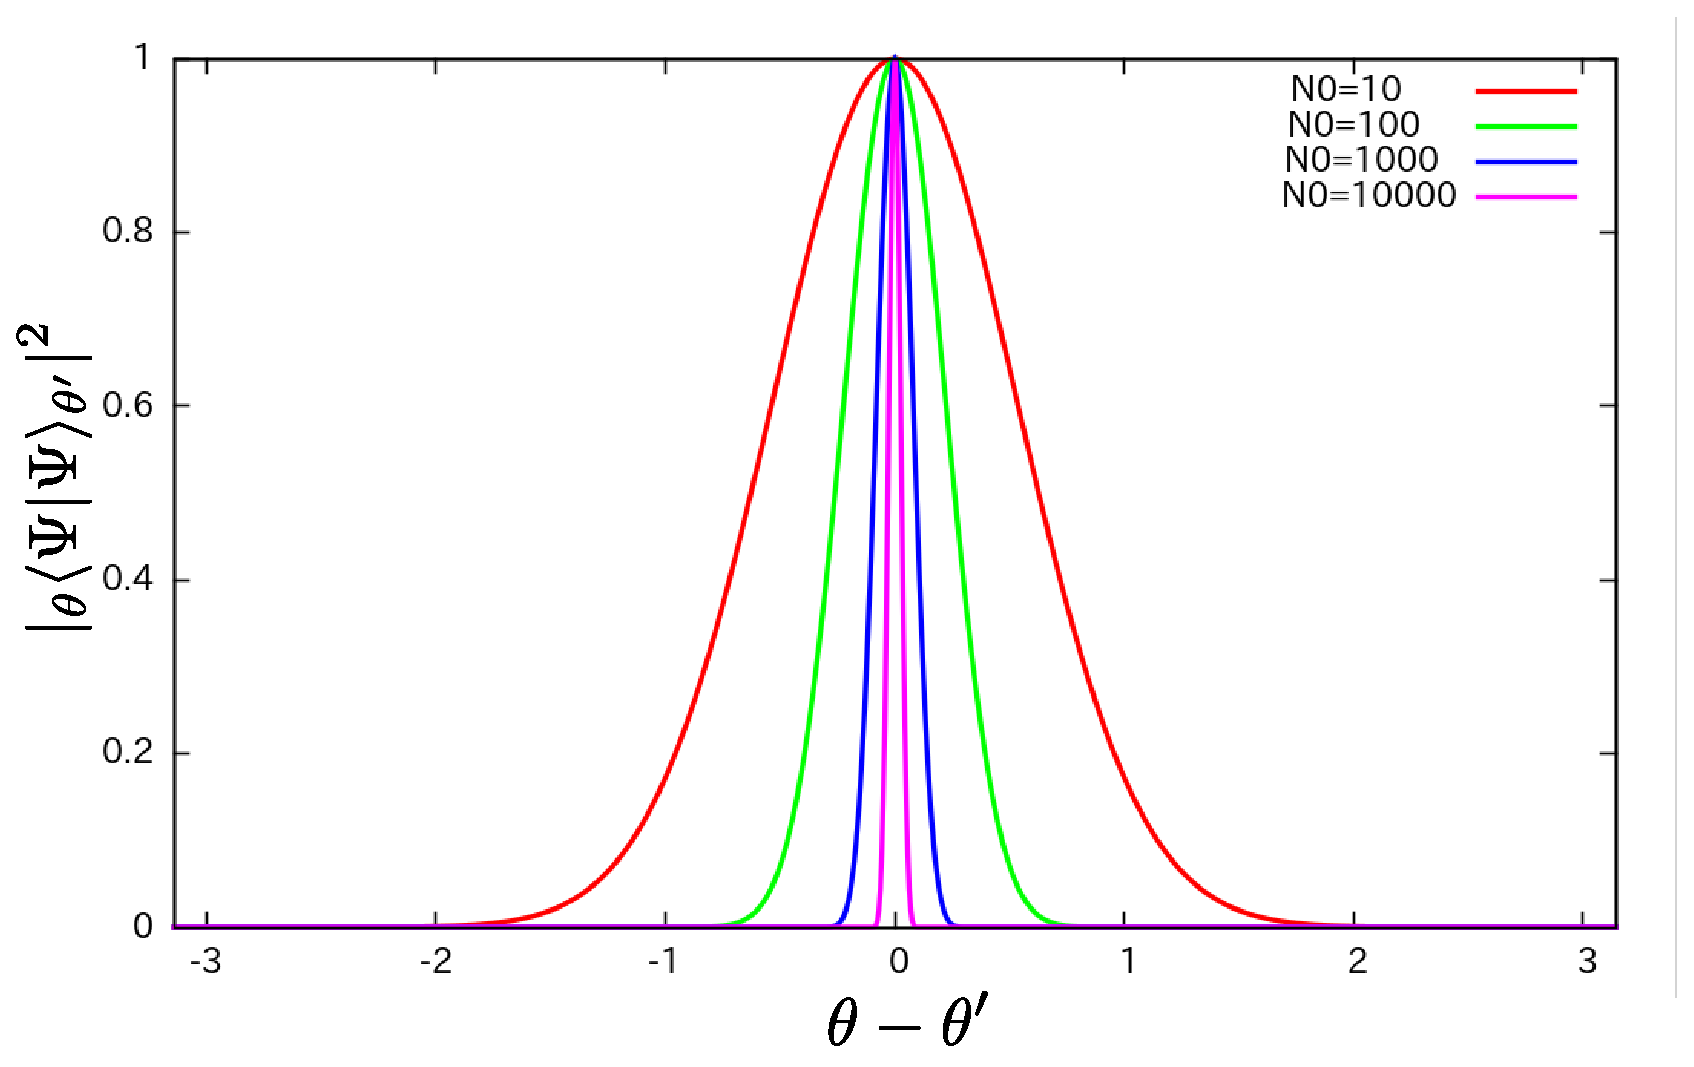
\includegraphics[width = 9cm]{./EPS/fig1.eps}
  \caption{相対位相と真空の直交性$(m=30)$}
  \label{fig1}
\end{figure}
\begin{comment}
  \begin{figure}[htbp]
    \centering
    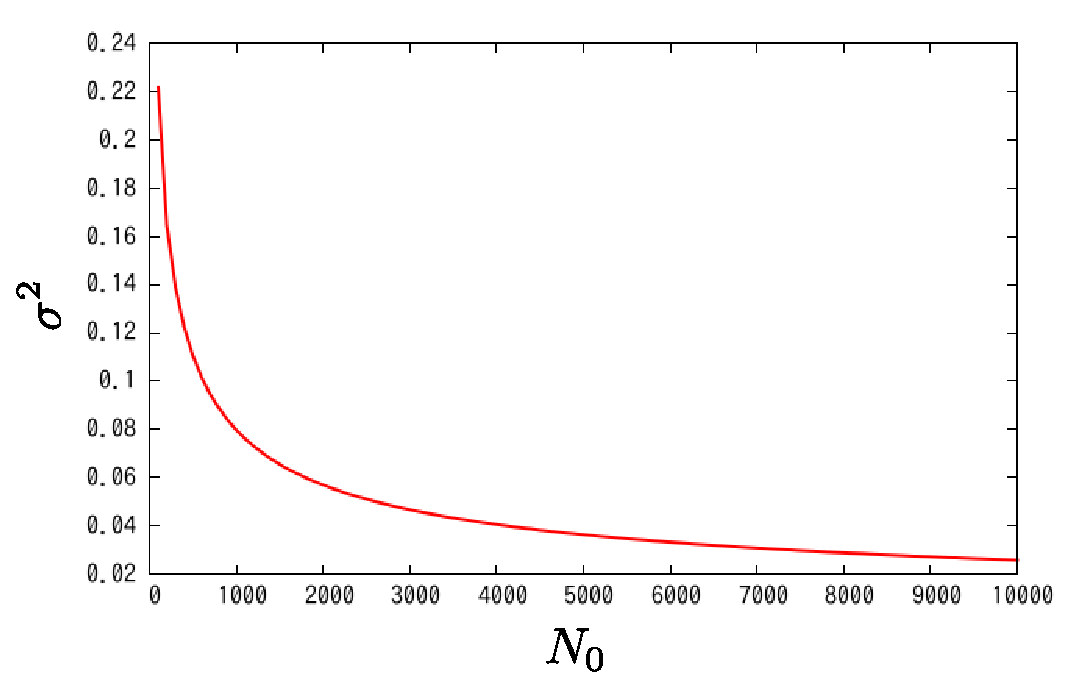
\includegraphics[width = 9cm]{./EPS/fig4.eps}
    \caption{真空の直交性の分散}
    \label{fig4}
  \end{figure}
\end{comment}
\begin{figure}[htbp]
  \centering
  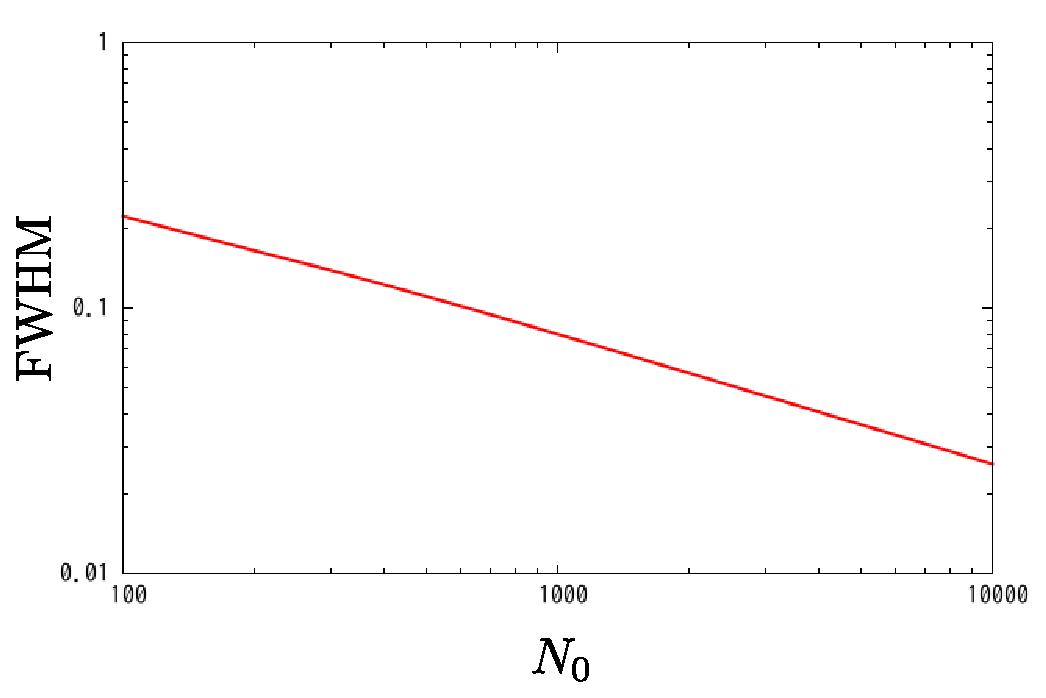
\includegraphics[width = 9cm]{./EPS/fig5.eps}
  \caption{真空の直交性の半値幅(両対数表示)}
  \label{fig5}
\end{figure}

$|_\theta\langle\Psi|\Psi\rangle_{\theta '}|^2$は$\theta=\theta'$において最大値1を取る.また$|\theta-\theta'|$に対して単調に減少し,
$N_0$が大きくなるとより早く減少する.同様に半値幅も$N_0$が大きくなるに従って減少していく様子が見られ,図\ref{fig1}のグラフは$\delta_{\theta\theta'}$に近付いていることがわかる.半値幅の両対数表示から算出した傾きは$-0.470...$だった.

\newpage
\subsection{位相演算子と位相ゆらぎ}
第4章の議論から,今回の定式化では$_\theta\langle\Psi|Q^2|\Psi\rangle_\theta \ll 1$の場合,$Q$は凝縮体の位相演算子とみなすことができる.凝縮体の位相にはゆらぎがあり,それは式(\ref{standard_deviation})で与えられる.この位相ゆらぎの$N_0$依存性を調べるために式(\ref{standard_deviation})を数値計算ができるように変形する:

\begin{eqnarray}
  \Delta Q &=& \sqrt{_\theta\langle\Psi|Q^2|\Psi\rangle_\theta}\\
  &=&\sqrt{_\theta\langle\Psi|\left[\frac{1}{2i\xi}\left(e^{2i\theta}b_\theta^\dagger - e^{-i\theta}b_\theta \right)\right]^2|\Psi\rangle_\theta}\\
  &=&\sqrt{-\frac{1}{4N_0}\  \!_\theta\langle\Psi|(e^{2i\theta}b_\theta^\dagger b_\theta^\dagger - b_\theta^\dagger b_\theta -b_\theta b_\theta^\dagger + e^{-2i\theta}b_\theta b_\theta)|\Psi\rangle_\theta}\\
  &=&\sqrt{-\frac{1}{4N_0}\sum_{mm'} \!_\theta\langle\Psi|m\rangle\langle m|(e^{2i\theta}b_\theta^\dagger b_\theta^\dagger - b_\theta^\dagger b_\theta -b_\theta b_\theta^\dagger + e^{-2i\theta}b_\theta b_\theta)|m'\rangle\langle m'|\Psi\rangle_\theta}\\
  %&=&\sqrt{-\frac{1}{4N_0}\sum_{mm'}\psi^*_{m,\theta}\left(e^{2i\theta}\sqrt{(m'+1)(m'+2)}\delta_{m,m'+2}-m'\delta_{mm'}-(m'+1)\delta_{mm'}+e^{-2i\theta}\sqrt{m'(m'-1)}\delta_{m,m'-2}\right)\psi_{m,\theta}}
  &=&\sqrt{\frac{1}{4N_0}\sum_{m}{\scriptstyle \left[(2m+1)\psi^*_{m,\theta}\psi_{m,\theta}-e^{2i\theta}\sqrt{(m-1)m}\psi^*_{m,\theta}\psi_{m-2,\theta}-e^{-2i\theta}\sqrt{(m+2)(m+1)}\psi^*_{m,\theta}\psi_{m+2,\theta}\right]}}\ \ \ \ \ \ \ \ \ \ \\
  &=&\sqrt{\frac{1}{4N_0}\sum_{m}{\scriptstyle \left[(2m+1)\psi^*_{m,\theta}\psi_{m,\theta}-e^{2i\theta}\sqrt{(m+2)(m+1)}\psi^*_{m+2,\theta}\psi_{m,\theta}-e^{-2i\theta}\sqrt{(m+2)(m+1)}\psi^*_{m,\theta}\psi_{m+2,\theta}\right]}}\ \ \ \ \ \ \ \ \ \ \\
  &=&\sqrt{\frac{1}{4N_0}\sum_m\left[(2m+1)\psi^*_{m,\theta}\psi_{m,\theta}-2{\rm Re}\left( e^{2i\theta}\sqrt{(m+2)(m+1)}\psi^*_{m+2,\theta}\psi_{m,\theta}\right)\right]}
\end{eqnarray}
\subsubsection{数値計算結果}
粒子数$N_0$と位相ゆらぎ$\Delta Q$の関係を図$\ref{fig3}$に示す.
\begin{comment}
  \begin{figure}[htbp]
    \centering
    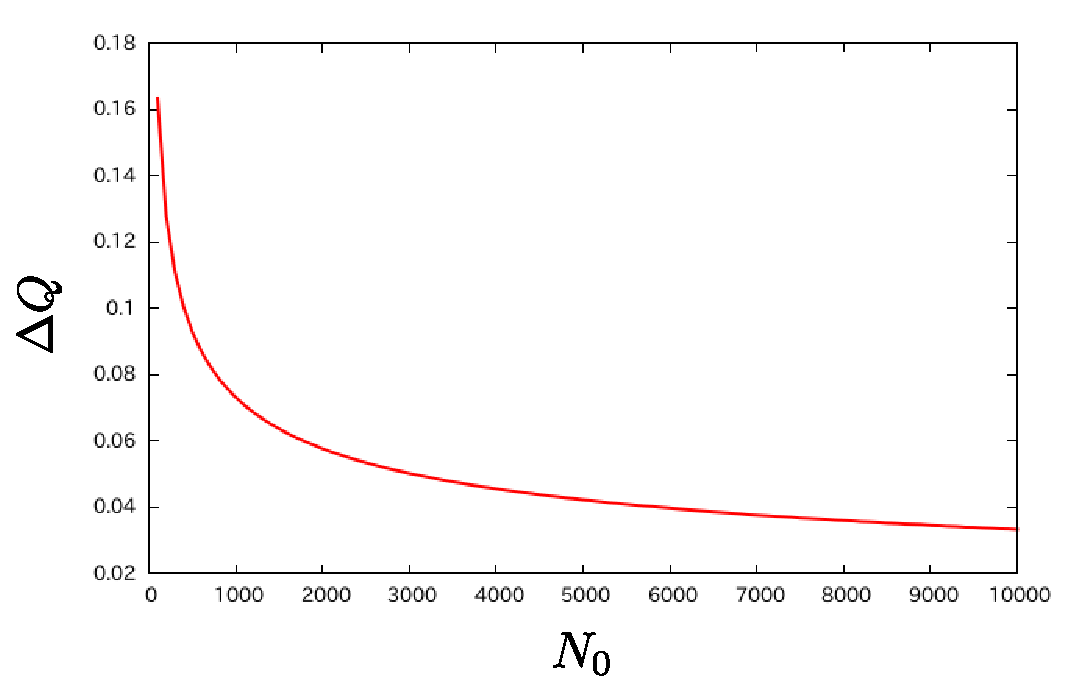
\includegraphics[width = 9cm]{./EPS/fig2.eps}
    \caption{粒子数と位相揺らぎ}
    \label{fig2}
  \end{figure}
\end{comment}
\begin{figure}[htbp]
  \centering
  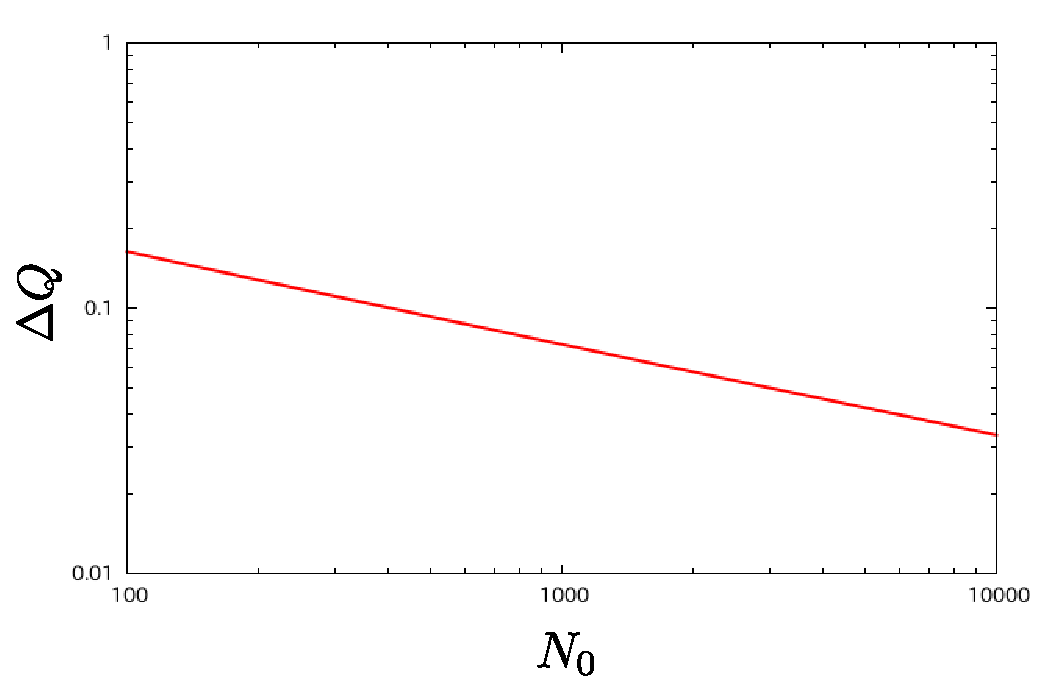
\includegraphics[width = 9cm]{./EPS/fig3.eps}
  \caption{粒子数と位相揺らぎ(両対数表示)}
  \label{fig3}
\end{figure}

図\ref{fig3}から算出した傾きは$-0.343...$だった.これは式(\ref{Q_variation})の見積りとほぼ一致していることがわかる.
\begin{comment}
  \subsection{真空の直交性と位相ゆらぎの相関}
  真空の直交性と位相ゆらぎに相関はあるだろうか.
  真空の$q$表示$\langle q|\Psi\rangle_\theta$の分散は位相ゆらぎを表していると考えると
  \begin{eqnarray}
    _\theta\langle\Psi|\Psi\rangle_{\theta'}=\int dq\  _\theta\langle\Psi|q\rangle\langle q|\Psi\rangle_{\theta'}
  \end{eqnarray}
  の式が示す通り,異なる位相を持つ真空同士の重なり積分は真空の直交性と関係がありそうである.よって,この重なり積分の$N_0$依存性を調べ,分散の変化を図\ref{fig5}と比較する.
  \subsubsection{計算結果}
  重なり積分の$N_0$依存性を図\ref{fig9},重なり積分と真空の直交性の分散の比較を図\ref{fig10}に示す.
  \begin{figure}[htbp]
    \centering
    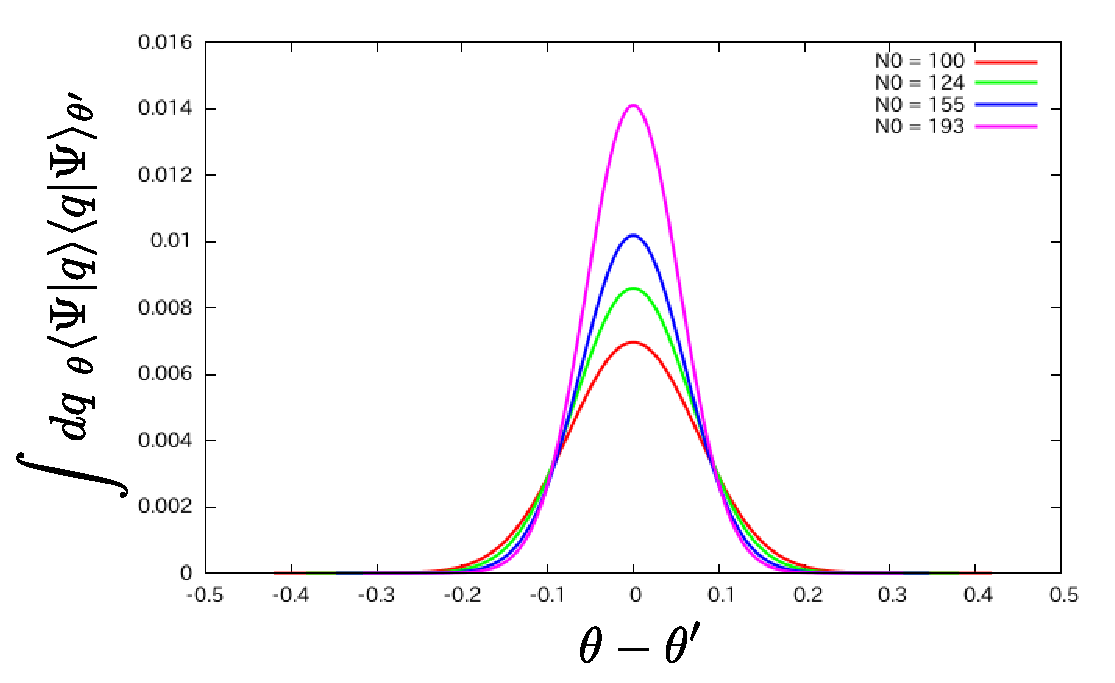
\includegraphics[width = 9cm]{./EPS/fig9.eps}
    \caption{重なり積分の$N_0$依存性}
    \label{fig9}
  \end{figure}
  \begin{figure}[htbp]
    \centering
    \includegraphics[width = 9cm]{./EPS/fig10.eps}
    \caption{重なり積分と直交性の分散}
    \label{fig10}
  \end{figure}
  重なり積分の分散の両対数表示における傾きは$-0.508$であり,真空の直交性の方と近い値が得られた.
\end{comment}
\begin{comment}
  \subsection{直交性と位相ゆらぎの関係}
  真空の直交性$_\theta\langle\Psi|\Psi\rangle_{\theta'}$に$q$の完全性を挿入する:
  \begin{eqnarray}
    _\theta\langle\Psi|\Psi\rangle_{\theta'} = \int dq\ _\theta\langle\Psi|q\rangle\langle q |\Psi\rangle_{\theta'}
  \end{eqnarray}
  真空の$q$表示$\langle q |\Psi\rangle_{\theta'}$の半値幅は位相ゆらぎと解釈でき,上式ではその重なり積分を計算している.
\end{comment}
\newpage
\section{結言}
本研究では場の演算子にゼロモードのみが現れ,空間自由度を持たないSingle mode模型を扱った.このモデルにおいて特定の条件のもとでゼロモード演算子$Q$が位相演算子と解釈できることを確認し,異なる位相を持つ真空同士の直交性・位相ゆらぎの計算を行った.凝縮体の位相ゆらぎが計算できること自体がひとつの成果である.

数値計算の結果,真空の直交性は凝縮粒子数を増加させると直交性が増し,$N_0 \rightarrow \infty$において$\delta_{\theta\theta'}$という理想と一致するような傾向が見られた.また数値計算で求めた位相ゆらぎは変分法で計算した値と良く一致した.
%%%%%%%%%%%%%%%%%%%%%%%%付録%%%%%%%%%%%%%%%%%%%%%%%%%%%%%%%
\section*{Appendix.A : 数値計算上の注意点}
\renewcommand{\theequation}{A.\arabic{equation}}
\subsection*{A.1  $m_{\rm max}$の値の設定}
一般に,素励起の最大数である$m_{\rm max}$は無限大に取るのが理想である.よって$m$に関する諸々の計算は$ \displaystyle \sum_{m=0}^{\infty}$とすべきだが,数値計算上では$ \displaystyle \sum_{m=0}^{m_{\rm max}}$とし,自己無撞着的に決定される$\delta \mu$が$m$に依存しなくなるような十分大きい$m_{\rm max}$を選ぶことにする.

$N_0$が大きくなるほど$\delta \mu$の収束性は悪くなるが,$N_0 = 10000$であれば$m=300$程度で十分収束していることが図$\ref{fig8}$からわかる.
\begin{figure}[htbp]
  \centering
  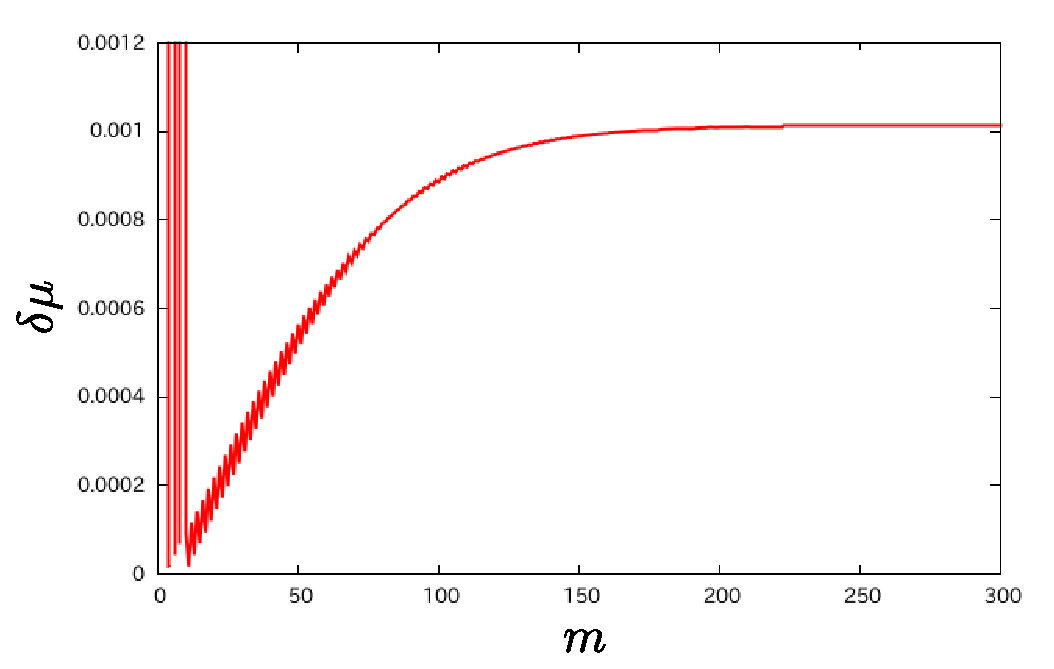
\includegraphics[width = 9cm]{./EPS/fig8.eps}
  \caption{$m$に対する$\delta \mu$の変化}
  \label{fig8}
\end{figure}
\subsection*{A.2  階乗の処理}
式(\ref{orthogonal})は数値計算可能な形ではあるが,階乗が含まれているのでdouble型ではオーバーフローを起こしてしまう.この問題を回避するためにさらに変形を施す.
\begin{eqnarray}
  z&\equiv&-ie^{i\bar \theta}|z|\\
  Z_{ml} &\equiv& \frac{1}{(m-l)!}\sqrt{\frac{m!}{l!}}|z|^{m-l}e^{-\frac{1}{4}|z|^2}
\end{eqnarray}
と置くと,式(\ref{orthogonal})は
\begin{eqnarray}
  _a\langle m|e^{\Xi_\theta}e^{-\Xi_{\theta'}}|m'\rangle_a
  =i^{m+m'}e^{i\bar \theta(m-m')}e^{r}\sum_{l=0}^{\min(m,m')}(-1)^l Z_{ml}Z_{m'l}
\end{eqnarray}
と書ける.$Z_{ml}$は
\begin{eqnarray}
  \nonumber
  Z_{ml} &=& \frac{\sqrt{_mP_{m-l}}}{(m-l)!}|z|^{m-l}\left(e^{-\frac{|z|^2}{4(m-l)}}\right)^{m-l}\\
  &=&\prod_{k=0}^{m-l-1}\left[\frac{\sqrt{m-k}}{m-l-k}|z|e^{-\frac{|z|^2}{4(m-l)}}\right]\label{Zml}
\end{eqnarray}
という形に変形することでdouble型のオーバーフローを防ぎながら計算することができる.
\subsection*{A.3  真空期待値のグラフにおける異常}
相対位相$\theta - \theta'$と真空期待値$|_\theta\langle\Psi|\Psi\rangle_{\theta'}|^2$の計算をする際には$\delta \mu$が収束する程度に$m_{\rm max}$を大きくしなければならないが,$m_{\rm max}$がある程度大きくなると$\theta - \theta'$が大きい範囲でグラフに図$\ref{fig6}$のような異常が見られる.この結果は$|_\theta\langle\Psi|\Psi\rangle_{\theta'}|^2 \leq \parallel\Psi_\theta\parallel^2\parallel\Psi_{\theta'}\parallel^2=1$を破っているので明らかに正しくない結果である.
\begin{figure}[htbp]
  \centering
  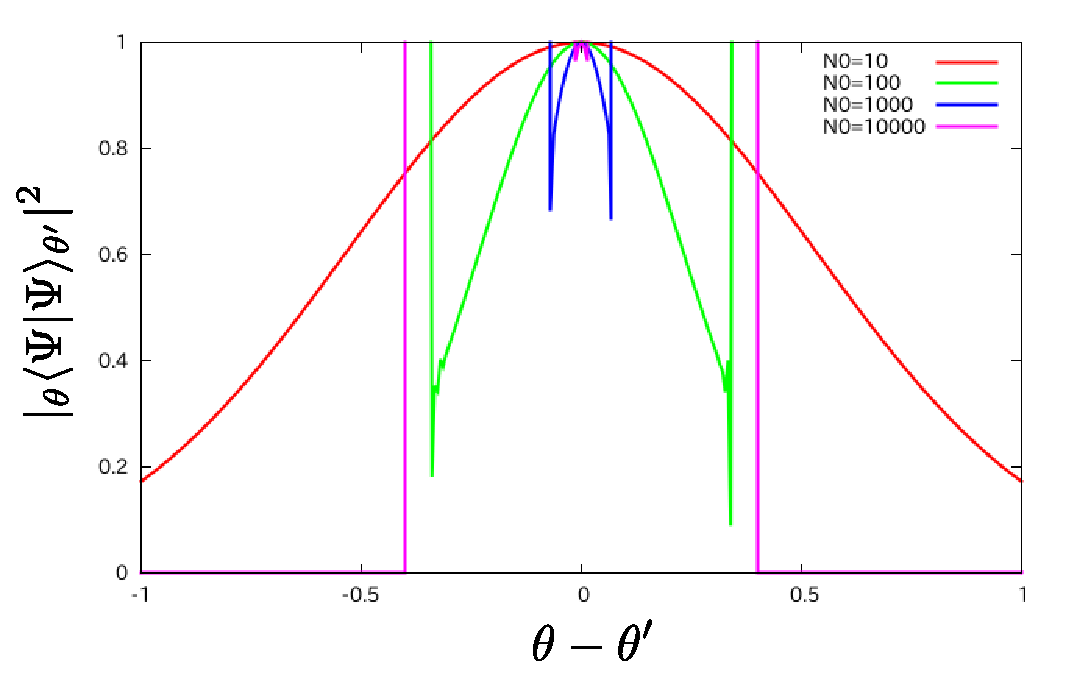
\includegraphics[width = 9cm]{./EPS/fig6.eps}
  \caption{相対位相と真空の直交性$(m=300)$}
  \label{fig6}
\end{figure}

この異常の原因のひとつは$Z_{ml}$である.double型のオーバーフローを避けるように計算をしたものの,$m=200$において$10^{40}$程度のオーダーを持つ.
%また$e^r=e^{-iN_0\sin(\theta - \theta')}$も,$N_0$について指数関数的に値を変えるので,$\theta-\theta'$がある程度の値を持てば全体に大きな影響を与える可能性がある.
本来であればこの項の影響は他のパラメータとの積で打ち消されるべきだが,数値計算上の桁落ち等の問題でうまく打ち消し合っていないことが問題であると思われる.この問題を回避するために5.2節では$\delta \mu$の決定以外では$m_{\rm max}=30$で計算するという手段を採用した.$m_{\rm max}$を小さくすることにより$Z_{ml}$の増加が抑制されている.

では今回の異常は本当に数値計算上の桁落ちによる問題なのだろうか.これを調べるために,式(\ref{Zml})による$Z_{ml}Z_{ml'}$をdouble型(64bit)のまま計算したものとfloat型(32bit)にキャストしたものを比較する.異常が起きている部分のグラフを図$\ref{fig7}$に示す.
グラフからfloat型の方がdouble型よりも$10^{10}$以上も大きな値を持っていることがわかり,これはfloat型にキャストしてから和を取ることによる誤差の蓄積が原因だと考えられる.つまり,有効数字が誤差に影響を与えているということであり,今回の異常は数値計算上の問題と捉えても良さそうである.
%桁落ちが問題になっているのであればこの2つの結果は違ったものになるはずである.
\begin{figure}[htbp]
  \centering
  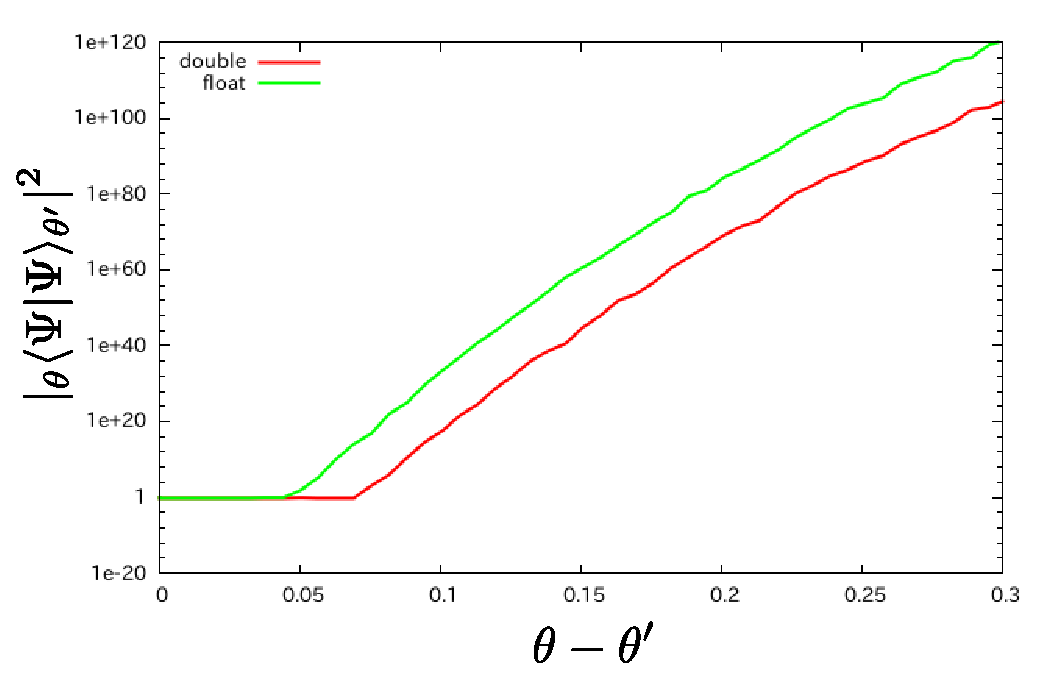
\includegraphics[width = 9cm]{./EPS/fig7.eps}
  \caption{double型とfloat型における真空期待値の比較(片対数表示)}
  \label{fig7}
\end{figure}

\renewcommand{\theequation}{\thechapter.\arabic{equation}}
\newpage
\section*{謝辞}
本研究を進めるにあたり、熱心にご指導を頂いた山中由也教授に感謝致します.中村祐介氏・高橋淳一氏には日々的確な助言を頂き,本研究に対する幅広いサポートをして頂きました.川口拓磨氏にはゼミ等を通じて数々の実りある示唆を頂きました.また,同期・同室の小山輝君・北原康貴君とは多くの議論を交わすことが出来ました.この場をお借りして深くお礼を申し上げます.
\begin{thebibliography}{99}
\bibitem{BEC} M. H. Anderson, J. R. Ensher, M. R. Matthews, C. E. Wieman, and E. A. Cornell, Science
  {\bf 269}, 198 (1995).
\bibitem{bogoliubov} N. N. Bogoliubov, J. Phys. (Moscow) {\bf 11}, 23 (1947).
\bibitem{de-gennes} P. G. de Gennes, Superconductivity of Metals and Alloys (Benjamin, New York, 1966).
\bibitem{nambu} Y. Nambu and G. Jona-Lasinio, Phys. Rev. {\bf 122}, 345 (1961).
\bibitem{goldstone} J. Goldstone, A. Salam, and S. Weinberg, Phys. Rev. {\bf 127}, 965 (1962).
\bibitem{lewenstein}M. Lewenstein and L. You, Phys. Rev. Lett. {\bf 77}, 3489 (1996).
\bibitem{matsumoto}H. Matsumoto and S. Sakamoto, Prog. Theor. Phys. {\bf 107}, 679 (2002).
\bibitem{mine}M. Mine, M. Okumura, and Y. Yamanaka, J. Math. Phys. {\bf 46}, 042307 (2005).
\bibitem{nakamura} Y. Nakamura, J. Takahashi, and Y. Yamanaka, Phys. Rev. A {\bf 89}, 013613 (2014).
\bibitem{andrews} M. R. Andrews, C. G. Townsend, H. J. Miesner, D. S. Durfee, D. M. Kurn, W. Ketterle, Science {\bf 275}, 589 (1997).
\bibitem{dirac} P. A. M. Dirac, Proc. R. Soc. London, Ser.\ {\bf A109}, 642 (1925).
\bibitem{igi} 猪木慶治, 川合光, 「基礎量子力学」, (講談社サイエンティフィク, 2007), pp. 170-175.
\end{thebibliography}

%%%%------------------------------------------------------------------------------------------------------------------------------------------------------------------------------------------------------------

\newpage
\chapter{研究 : 3次元一様有限温度系のゼロモード}
2015年度夏の学校. 有限温度ゼロモード系における自己無撞着計算がメイン. 有限温度系で重要な計算や考え方が頻出.

また, 夏の学校時点では凝縮粒子数の定義にゼロモード演算子の期待値を加えていなかったため, Depletionは相互作用定数$g$が小さいところで持ち上がる結果を得た. 凝縮粒子数の定義を変えたところ, Depletionは相互作用定数$g$に対してロバストになった. こっちのほうが自然だろうというのが今のところの結論. 
\section{問題設定}
粒子間の相互作用を考慮に入れてゼロモード演算子の期待値を計算をする.この効果のことを量子補正と呼ぶ.\\
相互作用がある場合はゼロ温度でも全ての粒子が凝縮するわけではないことから,今回は主に凝縮粒子数と非凝縮粒子数の割合(depletion)が相互作用によってどのように変わるか,またゼロモードの寄与がある場合とない場合で結果がどのように変わるかを見る.

まずは,量子補正を考慮した方程式の定式化から入る.
\subsection{冷却原子気体系のハミルトニアン}
冷却原子気体のハミルトニアンは以下のように与えられる.
\begin{eqnarray}
  H_{\rm H}=\int d\bm{x}\left[\psi_{\rm H}^\dagger(h_0-\mu)\psi_{\rm H} +\frac{g}{2}\psi_{\rm H}^\dagger\psi_{\rm H}^\dagger\psi_{\rm H}\psi_{\rm H}\right]
\end{eqnarray}
添字のHはHeisenberg描像であることを示している.$\mu$は化学ポテンシャル,$g$は相互作用定数,$h_0$は
\begin{eqnarray}
  h_0 = -\frac{\nabla^2}{2m}
\end{eqnarray}
であるような一様系を取り扱う.場の演算子$\psi_{\rm H}$は同時刻交換関係
\begin{eqnarray}
  &&\left[\psi_{\rm H}(\bm{x},t),\psi_{\rm H}^\dagger(\bm{x}',t) \right] = \delta(\bm{x} - \bm{x}')\\
  &&\left[\psi_{\rm H}(\bm{x},t),\psi_{\rm H}(\bm{x}',t) \right] = 0,\ \ \ \ \ \left[\psi_{\rm H}^\dagger(\bm{x},t),\psi_{\rm H}^\dagger(\bm{x}',t) \right] = 0
\end{eqnarray}
を満たす.このとき,$\psi_{\rm H}$は真空期待値を持つ:
\begin{eqnarray}
  \langle 0|\psi_{\rm H}(\bm{x})|0\rangle = \xi(\bm{x})\label{vaccum_ex1}
\end{eqnarray}
$\xi$は秩序変数と呼ばれ,$|\xi|^2$は凝縮体の密度と解釈できる.秩序変数は今回は時間に依存しないと仮定する.
場の演算子を以下のように分割する:
\begin{eqnarray}
  \psi_{\rm H} = \xi + \varphi_{\rm H}
\end{eqnarray}
$\xi$は凝縮体を記述する古典場,$\varphi_{\rm H}$は非凝縮体を記述する場の演算子と解釈できる.これは同時刻交換関係
\begin{eqnarray}
  \left[\varphi_{\rm H}(\bm{x},t),\varphi^\dagger_{\rm H}(\bm{x}',t)\right]  = \delta(\bm{x}-\bm{x}')\label{equal_time_commutation}
\end{eqnarray}
を満たしている.

ハミルトニアンを$\varphi_{\rm H}$の次数について整理すると
\begin{eqnarray}
  &&H_{{\rm H},1} = \int d\bm{x}\left[\varphi^\dagger_{\rm H}(h_0 - \mu + g|\xi|^2)\xi + \varphi_{\rm H}(h_0 - \mu + g|\xi|^2)\xi^*\right]\\
  &&H_{{\rm H},2} = \int d\bm{x}\left[\varphi^\dagger_{\rm H} {\cal L}\varphi_{\rm H} + \frac{1}{2}\varphi_{\rm H}{\cal M^*}\varphi_{\rm H}+\frac{1}{2}\varphi^\dagger_{\rm H}{\cal M}\varphi^\dagger_{\rm H}\right]\\
  &&H_{{\rm H},3} = g\int d\bm{x}\left[\xi^*\varphi^\dagger_{\rm H}\varphi_{\rm H}\varphi_{\rm H} + \xi\varphi^\dagger_{\rm H}\varphi^\dagger_{\rm H}\varphi_{\rm H} \right] \\
  &&H_{{\rm H},4} = \frac{g}{2}\int d\bm{x}\ \varphi^\dagger_{\rm H}\varphi^\dagger_{\rm H}\varphi_{\rm H}\varphi_{\rm H}
\end{eqnarray}
であり
\begin{eqnarray}
  {\cal L} = h_0 - \mu +2g|\xi|^2,\ \ \ \ \ {\cal M}=g\xi^2
\end{eqnarray}
である.

\subsection{相互作用描像}
系が十分低温であり相互作用$g$が小さいとする.この場合$H_{{\rm H},3},H_{{\rm H},4}$の効果は小さいとして,非摂動ハミルトニアンを$H_{{\rm H},u}=H_{{\rm H},1}+H_{{\rm H},2}$のように選び,Heisenberg描像から相互作用描像に移行する.まず
\begin{eqnarray}
  i\frac{d}{dt}U(t,t_0)=U(t,t_0)H_{{\rm H},p},\ \ \ \ \ U(t_0,t_0)=1,\ \ \ \ \ H_{{\rm H},p} = H_{\rm H} - H_{{\rm H},u}
\end{eqnarray}
を満たすようなユニタリー演算子$U(t,t_0)$を考え,Heisenberg描像の任意の演算子$A_{\rm H}(t)$を用いて相互作用描像の演算子を
\begin{eqnarray}
  A(t) = U(t,t_0)A_{\rm H}(t)U^{-1}(t,t_0)
\end{eqnarray}
と定義する.$t_0$はHeisenberg描像と相互作用描像が一致する時間である.Heisenberg方程式は
\begin{eqnarray}
  i\frac{d}{dt}A(t) = \left[A(t),H_u(t)\right]
\end{eqnarray}
である.ここで$A=H_u$と代入すると時間に依存しないことがわかるので,$H_u = H_{{\rm H},u}$である.

$U(t,t_0)$の時間発展は$H_{{\rm H},p}=H_{{\rm H},3}+H_{{\rm H},4}$に依存し,かつその効果が小さいことから場の演算子の摂動ゼロ次は
\begin{eqnarray}
  \langle0|\varphi_{\rm H}(x)|0\rangle = \langle0| U^{-1}(t,t_0)\varphi(x)U(t,t_0)|0\rangle \simeq \langle0|\varphi(x)|0\rangle
\end{eqnarray}
となっている.また相互作用描像のHeisenberg方程式より
\begin{eqnarray}
  i\frac{\partial}{\partial t}\varphi(x) = \left[\varphi(x),H_u\right]\label{Heisenberg}
\end{eqnarray}
であることがわかる.これ以降$x=(\bm{x},t)$とする.つまり,場の分割条件を
\begin{eqnarray}
  \langle0|\varphi_{\rm H}(x)|0\rangle \simeq \langle0|\varphi(x)|0\rangle = 0
\end{eqnarray}
とした場合,この性質が保存するためには式(\ref{Heisenberg})より
\begin{eqnarray}
  \bra{0}\left[\varphi(x),H_u\right]\ket{0} = 0
\end{eqnarray}
が必要となる.ここから定常Gross-Pitaevskii方程式(GP方程式)
\begin{eqnarray}
  \left[h_0 - \mu +g|\xi|^2\right]\xi = 0\label{GP}
\end{eqnarray}
が導かれる.
\subsection{量子補正}
量子補正を取り入れる場合は場の分割条件を$\bra{0}[\varphi,H_u]\ket{0}=0$ではなく
\begin{eqnarray}
  \bra{0}[\varphi,H]\ket{0} = 0 \label{split}
\end{eqnarray}
とする.これはもともとの場の分割条件$\bra{0}\varphi_H\ket{0} = 0$の摂動1次までを取り入れたことになっている\footnote{実は正確な表現ではない. }.これを具体的に計算する:
\begin{eqnarray}
  \nonumber  \bra{0}[\varphi,H_1]\ket{0} &=& \bra{0}\int d\bm{x}\left[\varphi,\left\{\varphi^\dagger{\cal L}\xi+\varphi{\cal L}\xi^*\right\}\right]\ket{0}\\
  &=& (h_0 - \mu + g|\xi|^2)\xi\\
  \nonumber  \bra{0}[\varphi,H_2]\ket{0} &=& \bra{0}\int d\bm{x}\left[\varphi,\left\{\varphi^\dagger{\cal L}\varphi+\frac{1}{2}\varphi{\cal M}^*\varphi + \frac{1}{2}\varphi^\dagger{\cal M}\varphi^\dagger\right\}\right]\ket{0}\\
  &=& \bra{0}{\cal L}\varphi + {\cal M}\varphi^\dagger \ket{0} = 0\\
  \nonumber  \bra{0}[\varphi,H_3]\ket{0} &=& \bra{0}g\int d\bm{x}\left[\varphi,\left\{\xi^*\varphi^\dagger\varphi\varphi + \xi\varphi^\dagger\varphi^\dagger\varphi \right\}\right]\ket{0}\\
  &=& g\bra{0}\varphi\varphi\ket{0}\xi^* + 2g\bra{0}\varphi^\dagger\varphi\ket{0}\xi\\
  \nonumber  \bra{0}[\varphi,H_4]\ket{0} &=& \bra{0}\frac{g}{2}\int d\bm{x}\left[\varphi,\varphi^\dagger\varphi^\dagger\varphi\varphi\right]\ket{0}\\
  &=& g\bra{0}\varphi^\dagger\varphi\varphi\ket{0}
\end{eqnarray}
ここで$\varphi$の3次の期待値の寄与は小さいものとすると,式(\ref{split})より
\begin{eqnarray}
  \left[h_0 - \mu + g|\xi|^2 + 2g\bra{0}\varphi^\dagger\varphi\ket{0}\right]\xi + g\bra{0}\varphi\varphi\ket{0}\xi^* = 0
\end{eqnarray}
これが量子補正を考慮したGP方程式である.ここでゼロモード部と励起部に分けて記述すると
\begin{eqnarray}
  \nonumber \bra{0}\varphi^\dagger\varphi\ket{0} &=& _{\rm ex}\bra{0}\varphi^\dagger_{\rm ex}\varphi_{\rm ex}\ket{0}_{\rm ex} + |\xi|^2\bra{\Psi}Q^2\ket{\Psi} + |\eta|^2\bra{\Psi}P^2\ket{\Psi} \\
  &&\ \ \ \ \ \ \ \ -{\rm Re}\xi^*\eta -{\rm Im}\xi^*\eta(QP + PQ)\\
  \nonumber  \bra{0}\varphi\varphi\ket{0} &=& _{\rm ex}\bra{0}\varphi_{\rm ex}\varphi_{\rm ex}\ket{0}_{\rm ex} - \xi^2\bra{\Psi}Q^2\ket{\Psi} + \eta^2\bra{\Psi}P^2\ket{\Psi} \\
  &&\ \ \ \ \ \ \ \ -i\xi\eta\bra{\Psi}QP + PQ\ket{\Psi}
\end{eqnarray}
となる.ここで$\varphi = -iQ\xi + P\eta + \varphi_{\rm ex}$とし,かつ$\ket{0} = \ket{0}_{\rm ex}\otimes\ket{\Psi}$としている.$Q,P$は正準交換関係$[Q,P] = i$を満たすゼロモード演算子,非摂動ハミルトニアン$H_u$の励起部$H_u^{\rm ex}$,ゼロモード部$H_u^{QP}$の固有状態をそれぞれ$\ket{0}_{\rm ex},\ket{\Psi}$である.

GP方程式が補正を受けたので,Bogoliubov-de Gennes方程式(BdG方程式)にも補正を加える.具体的には
\begin{eqnarray}
  {\cal L} &=&  h_0 - \mu + 2g(|\xi|^2 + \bra{0}\varphi^\dagger\varphi\ket{0})\label{L}\\
  {\cal M} &=& g(\xi^2 - \bra{0}\varphi\varphi\ket{0})\label{M}
\end{eqnarray}
となっていれば$\bm{y}_0 = \begin{pmatrix}\xi & -\xi^*  \end{pmatrix}$がゼロモードであることを守れる.ここで非摂動ハミルトニアンを
\begin{eqnarray}
  H_u = H_1 + H_2 + [H_3 + H_4]_{QP} -\delta\mu P -\delta\nu Q + \delta H
\end{eqnarray}
と取り,カウンター項$\delta H$を
\begin{eqnarray}
  \delta H = g\int d\bm{x}\left[2\varphi^\dagger\varphi\bra{0}\varphi^\dagger\varphi\ket{0}-\frac{1}{2}\varphi\varphi\bra{0}\varphi^\dagger\varphi^\dagger\ket{0}-\frac{1}{2}\varphi^\dagger\varphi^\dagger\bra{0}\varphi\varphi\ket{0}\right]
\end{eqnarray}
と選ぶことで,$H_u^{QP}$は量子補正を考慮しない場合と同じ形を取ることができる.式(\ref{L})(\ref{M})より共役モード方程式$
\begin{pmatrix}
  {\cal L} & {\cal M}\\
  -{\cal M}&-{\cal L}
\end{pmatrix}
\bm{y}_{-1}=I\bm{y}_0
$は
\begin{eqnarray}
  \left[h_0 - \mu + 2g(|\xi|^2 + \bra{0}\varphi^\dagger\varphi\ket{0})\right]\eta + g(\xi^2 - \bra{0}\varphi\varphi\ket{0})\eta^*=I\xi
\end{eqnarray}
となる.以上の定式化を用いて各物理量の計算を行っていく.
\section{自己無撞着ループ}
前節で導いた関係式に現れる物理量は自己無撞着に決定されるが,その関係式同士のつながりは複雑である.
以下では3次元一様有限温度系に現れる自己無撞着ループについてまとめる.2章のはなしを有限温度に拡張するために期待値のとり方を変えていることに注意.
\\

\begin{itembox}[c]{0. 初期設定}
  \begin{center}
    $V_t = \ev{\varphi^{\dagger}\varphi} = 0$, $V_a = \ev{\varphi\varphi} = 0$からスタート
  \end{center}
\end{itembox}

\begin{center}
  $\Downarrow$
\end{center}

\begin{itembox}[c]{1. GP方程式}
  \begin{center}
    GP方程式より$\xi, \mu $を求める
  \end{center}
\end{itembox}

\begin{center}
  $\Downarrow$
\end{center}

\begin{itembox}[c]{2. 共役モード方程式}
  \begin{center}
    共役モード方程式より$\eta, I$を求める
  \end{center}
\end{itembox}

\begin{center}
  $\Downarrow$
\end{center}

\begin{itembox}[c]{3. BdG方程式}
  \begin{center}
    BdG方程式(Bogoliubov変換)より$u_l, v_l$を求める
  \end{center}
\end{itembox}

\begin{center}
  $\Downarrow$
\end{center}

\begin{itembox}[c]{4. ゼロモード方程式}
  \begin{center}
    ゼロモード方程式より固有関数$\ev{q|\Psi}$を求め,$\ev{P}$を求める\\
    $\Updownarrow$\\
    $\ev{P} = 0$となるように自己無撞着に$\delta\mu$を決定
  \end{center}
\end{itembox}

\begin{center}
  $\Downarrow$
\end{center}

\begin{itembox}[c]{5. ゼロモード演算子}
  \begin{center}
    $\ev{Q^2}, \ev{P^2}$を求める
  \end{center}
\end{itembox}

\begin{center}
  $\Downarrow$
\end{center}

\begin{itembox}[c]{6. 熱平均・異常平均}
  \begin{center}
    $V_t, V_a$を求める.
  \end{center}
\end{itembox}

\begin{center}
  $\Downarrow$
\end{center}

\begin{itembox}[c]{ループ/終了条件}
  \begin{center}
    「1. GP方程式」 に戻って計算を繰り返す.$V_t, V_a$の値が変化しなくなったら終了.
  \end{center}
\end{itembox}

\subsection{GP方程式}
入力:$V_t,V_a$

$\xi,\eta$は実数とする.量子補正を含むGP方程式は
\begin{eqnarray}
  [-\mu + g\xi^2 + g(2V_t + V_a)]\xi = 0
\end{eqnarray}  
である.今回は一様系を扱うため微分項$h_0$がなくなり,簡単な代数方程式になる.これを$\mu$について解く:
\begin{eqnarray}
  \mu = g(\xi^2 + 2V_t + V_a)
\end{eqnarray}
ここで粒子数$N$が保存するためには
\begin{eqnarray}
  \nonumber  N &=& \int d\bm{x}\ev{\psi^\dagger\psi}\\
  \nonumber  &=& \int d\bm{x}\ev{(\xi + \varphi^\dagger)(\xi + \varphi)}\\
  &=& V(\xi^2 + V_t)
\end{eqnarray}
を満たさなければならない.ここでは分割条件から$\ev{\varphi},\ev{\varphi^\dagger}$はゼロになっている.したがって,
\begin{itembox}[c]{GP方程式}
  \begin{eqnarray}
    \xi &=& \sqrt{\frac{N}{V} - V_t}\\
    \mu &=& g(\frac{N}{V} + V_t + V_a)
  \end{eqnarray}
\end{itembox}
となることがわかる.

\subsection{共役モード方程式}
入力:$V_a, V_t, \xi, \mu$

量子補正を含む共役モード方程式は
\begin{eqnarray}
  [-\mu + g(3\xi^2 + 2V_t - V_a)]\eta = I\xi 
\end{eqnarray}
である.GP方程式と同様の理由で代数方程式となっている.これを$I$について解く:
\begin{eqnarray}
  I = \frac{\eta}{\xi}[-\mu + g(3\xi^2 + 2V_t - V_a)]
\end{eqnarray}
ここでゼロモードと共役モードの規格化条件から
\begin{eqnarray}
  \nonumber  (\bm{y}_0, \bm{y}_{-1}) &=& \int d\bm{x}
  \begin{pmatrix}
    \xi & -\xi
  \end{pmatrix}
  \begin{pmatrix}
    1 & 0\\
    0 & -1
  \end{pmatrix}
  \begin{pmatrix}
    \eta\\
    \eta
  \end{pmatrix}\\
  &=& 2V\xi\eta = 1
\end{eqnarray}
を満たさなければならない.したがって
\begin{itembox}[c]{共役モード方程式}
  \begin{eqnarray}
    \eta &=& \frac{1}{2V\xi}\\
    I &=& \frac{-\mu + g(3\xi + 2V_t - V_a)}{2V\xi^2}
  \end{eqnarray}
\end{itembox}
となることがわかる.

\subsection{BdG方程式}
入力:$V_a, V_t, \xi, \mu$

一様系ではBogoliubov変換から$u_l,v_l$を求めることができる.

\begin{eqnarray}
  \varphi = \frac{1}{(2\pi)^{3/2}}\int d\bm{k}\ b_{\bm{k}}e^{i\bm{k}\bm{x}}
\end{eqnarray}
と展開すると,ハミルトニアンの2次$H_2$は
\begin{eqnarray}
  H_2 = \frac{1}{2}\int d\bm{k}\ [2{\cal L}_kb^\dagger_{\bm{k}}b_{\bm{k}} + {\cal M}(b^\dagger_{\bm{k}}b^\dagger_{-\bm{k}} + b_{\bm{k}}b_{-\bm{k}})]
\end{eqnarray}
とかける.ただし
\begin{eqnarray}
  {\cal M} &=& g(\xi^2 - V_a)\\
  \nonumber  {\cal L}_k &=& \frac{\hbar^2}{2m}k^2 - \mu + 2g(\xi^2 + V_t)\\
  &=& \frac{\hbar^2}{2m}k^2 + {\cal M}
\end{eqnarray}
である.ここで
\begin{eqnarray}
  H_2 = \int d\bm{k}\ \omega_ka^\dagger_{\bm k}a_{\bm k}
\end{eqnarray}
となるような
\begin{eqnarray}
  a_{\bm k} = u_kb_{\bm k} - v_kb_{-\bm{k}}\label{operator}
\end{eqnarray}
を満たす$u_k$, $v_k$を探す.$a_k$は生成消滅演算子の代数を満たさなければならないので
\begin{eqnarray}
  |u_k|^2-|v_k|^2=1
\end{eqnarray}
が必要であり,式(\ref{operator})を$b$について解いて$H_2$に代入することにより,対角化の条件は
\begin{eqnarray}
  2{\cal L}_ku_kv_k -{\cal M}(u^2_k + v^2_k) = 0
\end{eqnarray}
であることがわかる.これらを連立させることにより
\begin{itembox}[c]{Bogoliubov変換}
  \begin{eqnarray}
    \begin{pmatrix}
      u_k\\
      v_k
    \end{pmatrix}
    &=& \frac{1}{\sqrt{2\omega_k}}
    \begin{pmatrix}
      \sqrt{{\cal L}_k + \omega_k}\\
      -\sqrt{{\cal L}_k - \omega_k}
    \end{pmatrix}\\
    \omega_k &=& \sqrt{{\cal L}^2_k - {\cal M}^2}
  \end{eqnarray}
\end{itembox}
を得る.
\subsection{ゼロモード方程式}
入力:\ $\xi, \eta, I$

今回考えるゼロモード方程式は以下:
\begin{eqnarray}
  H_u^{QP}\ket{\Psi_m} = E_m\ket{\Psi_m}
\end{eqnarray}
ただし
\begin{eqnarray}
  \nonumber  H_u^{QP} = -(\delta\mu + 4C)P &+& \frac{I-4D}{2}P^2 + 2BQPQ + 2DP^3\\
  &+& \frac{1}{2}AQ^4 -2BQ^2 + CQP^2Q + \frac{1}{2}EP^4
\end{eqnarray}
である.これを$q$空間で差分化して数値的に解く.$q$空間での波束の幅はおよそ$N_0^{-1/3}$のオーダーであることを基に系のサイズを決める.
\\
\begin{eqnarray}
  \Psi_q = \sqrt{\Delta q}\ev{q|\Psi}
\end{eqnarray}
として差分化すると,ハミルトニアン$H_u^{QP}$は以下のようになる
\begin{eqnarray}
  H_u^{QP} =
  \begin{pmatrix}
    \alpha_0 & \beta_0& \gamma_0& & & \\
    \beta_0^* & \alpha_1 & \beta_1 & \gamma_1 & & \\
    \gamma_0^* &\beta_1^* &\alpha_2 &\beta_2 &\gamma_2 &\\
    &\gamma_1^* & \beta_2^* & \alpha_3 & \ddots & \ddots\\
    & & \gamma_2^* & \ddots &\ddots &\ddots \\
    &&&\ddots &\ddots &\ddots 
  \end{pmatrix}
\end{eqnarray}
\begin{eqnarray}
  \alpha_q &=& \frac{3E}{\Delta q^4} + \frac{I-4D}{\Delta q^2} + (2C -2\Delta q^2B)(q-\frac{N_q}{2})^2 + \frac{\Delta q^4}{2}Aq^4 \\
  \beta_q &=& -\frac{2E}{\Delta q^4} - \frac{2iD}{\Delta q^3} - \frac{I-4D}{2\Delta q^2} + \frac{i(\delta\mu + 4C)}{2\Delta q} - (C + i\Delta qB)(q - \frac{N_q}{2})(q - \frac{N_q}{2}+1)\\
  \gamma_q &=& \frac{E}{2\Delta q^4} + \frac{iD}{\Delta q^3}
\end{eqnarray}
有限温度系での期待値の取り方に注意すると
\begin{eqnarray}
  \nonumber  \ev{P} &=& \frac{{\rm Tr}\rho P}{{\rm Tr}\rho}\\
  \nonumber &=& \frac{\sum_m\bra{\Psi_m} P \ket{\Psi_m}e^{-\beta E_m}}{\sum_me^{-\beta E_m}}\\
  &=& \frac{\sum_m\sum_q{\rm Im} \Psi_q^{*,m}\Psi_{q+1}^me^{-\beta E_m}}{\Delta q\sum_me^{-\beta E_m}}
\end{eqnarray}
ただし密度演算子$\rho$は
\begin{eqnarray}
  \rho = e^{-\beta H_u^{QP}}
\end{eqnarray}
である.場の分割条件から$\ev{P} = 0$を満たさなければならないので,それに合わせて自己無撞着的に$\delta\mu$を決定することになる.数値計算上では二分法を用いる.

\subsection{$\ev{Q^2},\ev{P^2}$の計算}

前節で決定された$\delta \mu$を基に求めたゼロモード固有関数$\Psi^m_q$を用いて$\ev{P}$と同様の計算で$\ev{Q^2},\ev{P^2}$を求める.
\begin{itembox}[c]{ゼロモード演算子の有限温度期待値}
  \begin{eqnarray}
    \ev{Q^2}&=& \frac{\Delta q^2\sum_m\sum_q(q - \frac{N_q}{2})|\Psi_q^m|^2e^{-\beta E_m}}{\sum_me^{-\beta E_m}}\\
    \ev{P^2}&=& \frac{2\sum_m\sum_q(|\Psi_q^m|^2-{\rm Re}\Psi_q^{*,m}\Psi_{q+1}^m)e^{-\beta E_m}}{\Delta q^2\sum_me^{-\beta E_m}}
  \end{eqnarray}
\end{itembox}

\subsection{熱平均$V_t$・異常平均$V_a$}
入力:$\xi, \eta, u_l, v_l, \ev{Q^2}, \ev{P^2}$

熱平均・異常平均は以下の通り:
\begin{eqnarray}
  V_t = \ev{\varphi^\dagger\varphi} &=& _{{\rm ex}}\ev{\varphi^\dagger_{{\rm ex}}\varphi_{{\rm ex}}}_{{\rm ex}} + \xi^2\ev{Q^2} + \eta^2\ev{P^2} -\xi\eta \\
  %  &=& \sum_l\left[\frac{1}{e^{\beta\omega_l}-1}(|u_l|^2 + |v_l|^2)\right] + \xi^2\ev{Q^2} + \eta^2\ev{P^2} -\xi\eta 
  V_a = \ev{\varphi\varphi} &=& _{{\rm ex}}\ev{\varphi_{{\rm ex}}\varphi_{{\rm ex}}}_{{\rm ex}} - \xi^2\ev{Q^2} + \eta^2\ev{P^2} + i\xi\eta\ev{QP+PQ} 
  %  &=& \sum_l\left[\left(\frac{2}{e^{\beta\omega_l}-1}+1\right)u_lv^*_l\right] - \xi^2\ev{Q^2} + \eta^2\ev{P^2} + i\xi\eta\ev{QP+PQ} 
\end{eqnarray}
$\varphi_{\rm ex}$を以下のように展開する:
\begin{eqnarray}
  \varphi_{\rm ex} = \frac{1}{\sqrt{(2\pi)^3}}\int^{\infty}_{-\infty} d\bm{k}[a_{\bm{k}}u_k + a^\dagger_{-\bm{k}} v_k^*]e^{i\bm{k}\bm{x}}
\end{eqnarray}
ここで$a_{\bm{k}}$が消去する真空を$\ket{0}_k$,粒子数状態を
\begin{eqnarray}
  \ket{n} = \ket{n_1}_1\otimes\ket{n_2}_2\otimes\ket{n_3}_3\otimes... = \underset{k}{\otimes}\ket{n_k}_k
\end{eqnarray}
とする.

以上から$_{\rm ex}\ev{\varphi^\dagger_{{\rm ex}}\varphi_{{\rm ex}}}_{\rm ex},\  _{\rm ex}\ev{\varphi_{{\rm ex}}\varphi_{{\rm ex}}}_{\rm ex}$の計算をしていくために励起モードの期待値計算についてまとめる.
\begin{eqnarray}
  _{\rm ex}\ev{A}_{\rm ex} = \frac{{\rm Tr}\rho A}{{\rm Tr}\rho},\ \ \ \ \ \rho = e^{-\beta H^{\rm ex}_u}
\end{eqnarray}
であり
\begin{eqnarray}
  \nonumber  {\rm Tr}\rho &=& \sum_{n_1}\sum_{n_2}...\bra{n}e^{-\beta\sum_k\omega_{\bm{k}}a^\dagger_{\bm{k}}a_{\bm{k}}}\ket{n} = \sum_{n_1}\sum_{n_2}...\bra{n}e^{-\beta\sum_k\omega_{\bm{k}}n_{\bm{k}}}\ket{n} = \sum_{n_1}\sum_{n_2}...\prod_ke^{-\beta\omega_{\bm{k}}n_{\bm{k}}}\\
  &=& \prod_k\sum_{n_1}\sum_{n_2}...e^{-\beta\omega_{\bm{k}}n_{\bm{k}}} = \prod_k\sum_{n_{\bm{k}}}e^{-\beta\omega_{\bm{k}}n_{\bm{k}}} = \prod_k\frac{1}{1-e^{-\beta\omega_{\bm{k}}}}
\end{eqnarray}
\begin{eqnarray}
  \nonumber  {\rm Tr}\rho a^\dagger_{\bm k}a_{\bm{k}} &=& \sum_{n_1}\sum_{n_2}...\bra{n}e^{-\beta\sum_k\omega_{\bm{k}}a^\dagger_{\bm k}a_{\bm{k}}}a^\dagger_{\bm k}a_{\bm{k}}\ket{n} = \sum_{n_1}\sum_{n_2}...\left(\prod_{l\neq k}e^{-\beta\omega_ln_l}\right)n_le^{-\beta\omega_ln_l}\\
  \nonumber  &=& \prod_{l\neq k}\left(\sum_{n_1}\sum_{n_2}...\sum_{n_{l-1}}\sum_{n_{l+1}}...e^{-\beta\omega_ln_l}\right)\sum_kn_{\bm{k}}e^{-\beta\omega_{\bm{k}}n_{\bm{k}}} = \left(\prod_{k\neq l}\sum_{n_{\bm{k}}}e^{-\beta\omega_ln_l}\right)\sum_kn_{\bm{k}}e^{-\beta\omega_{\bm{k}}n_{\bm{k}}}\\
  &=&\left(\prod_{l\neq k}\frac{1}{1-e^{-\beta\omega_l}}\right)\frac{e^{-\beta\omega_{\bm{k}}}}{(1-e^{-\beta\omega_{\bm{k}}})^2}
\end{eqnarray}
から,
\begin{eqnarray}
  \nonumber  _{\rm ex}\ev{a^\dagger_{\bm{k}}a_{\bm{k}}}_{\rm ex} &=&  \frac{{\rm Tr}\rho a^\dagger_{\bm k}a_{\bm{k}}}{{\rm Tr}\rho}\\
  \nonumber &=& \frac{\left(\prod_{l\neq k}\frac{1}{1-e^{-\beta\omega_l}}\right)\frac{e^{-\beta\omega_{\bm{k}}}}{(1-e^{-\beta\omega_{\bm{k}}})^2}}{\prod_k\frac{1}{1-e^{-\beta\omega_{\bm{k}}}}}\\
  &=&\frac{1}{e^{\beta\omega_{\bm{k}}}-1}\\
  _{\rm ex}\ev{a^\dagger_{\bm{k}}a^\dagger_{-\bm{k}}}_{\rm ex} &=& _{\rm ex}\ev{a_{\bm{k}}a_{-\bm{k}}}_{\rm ex} = 0
\end{eqnarray}
となる.これはBose-Einstein分布関数である. ただし, これは$\bm{k}$が離散の場合である. $\bm{k}$が連続の場合は以下のように拡張する\footnote{付録参照}:
\begin{eqnarray}
  _{\rm ex}\ev{a_{\bm k}^\dagger a_{\bm{k}'}}_{\rm ex} = \frac{1}{e^{\beta\omega_{\bm{k}}}-1}\delta(\bm{k} - \bm{k}')
\end{eqnarray}
これより
\begin{eqnarray}
  \nonumber  _{\rm ex}\ev{\varphi^\dagger_{\rm ex}\varphi_{\rm ex}}_{\rm ex} &=& \frac{1}{(2\pi)^3}\int^{\infty}_{-\infty}  d \bm{k}' d \bm{k}\ {_{\rm ex}\ev{(a_{\bm{k}'}u_{k'}+a^\dagger_{-\bm{k}'}v^*_{k'})^\dagger(a_{\bm{k}}u_k+a^\dagger_{-\bm{k}}v^*_k)}_{\rm ex}}e^{i(\bm{k}-\bm{k}')\bm{x}}\\
  \nonumber  &=& \frac{1}{(2\pi)^3}\int^{\infty}_{-\infty} d \bm{k}' d \bm{k}\left[{_{\rm ex}\ev{a^\dagger_{\bm{k}}a_{\bm{k}}}_{\rm ex}}u^*_ku_k + {_{\rm ex}\ev{a_{-\bm{k}}a^\dagger_{-\bm{k}}}_{\rm ex}}v_kv^*_k\right]\delta(\bm{k}-\bm{k}')e^{i(\bm{k}-\bm{k'})\bm{x}}\\
  &=& \frac{1}{(2\pi)^3}\int^{\infty}_{-\infty} d\bm{k}\left[\frac{1}{e^{\beta\omega_{\bm{k}}}-1}(|u_k|^2+|v_k|^2)+|v_k|^2\right]
\end{eqnarray}
となり,同様の計算により
\begin{eqnarray}
  _{{\rm ex}}\ev{\varphi_{{\rm ex}}\varphi_{{\rm ex}}}_{{\rm ex}} &=& \frac{1}{(2\pi)^3}\int^\infty_{-\infty} d\bm{k}\left[\left(\frac{2}{e^{\beta\omega_k}-1}+1\right){\rm Re}u_kv^*_k\right]
\end{eqnarray}
であることもわかる.ここに$u_k,v_k$の値を代入して$(k_x, k_y, k_z)$から$(k, \theta, \phi)$の変数変換を施すと
\begin{itembox}[c]{熱平均・異常平均}
  \begin{eqnarray}
    _{\rm ex}\ev{\varphi^\dagger_{\rm ex}\varphi_{\rm ex}}_{\rm ex} &=& \frac{1}{(2\pi)^2} \int^{\infty}_0 dk\ \frac{k^2}{\omega_k}\left[\frac{2\Lk}{e^{\beta\omega_k} - 1} + \Lk - \omega_k\right]\\
    _{\rm ex}\ev{\varphi_{\rm ex}\varphi_{\rm ex}}_{\rm ex} &=& -\frac{1}{(2\pi)^2} \int^{\infty}_0 dk\ \frac{k^2\M}{\omega_k}\left[\frac{2}{e^{\beta\omega_k}-1}+1\right]
  \end{eqnarray}
\end{itembox}
であることがわかる.これらをSimpson積分することで$V_t,\ V_a$を計算する.
\subsubsection{積分範囲の設定}
数値計算上では無限大の積分は不可能なので,適当な値で積分を打ち切る必要がある.$_{\rm ex}\ev{\varphi^\dagger_{\rm ex}\varphi_{\rm ex}}_{\rm ex}$の被積分関数は遠方で収束するので問題ない一方,$_{\rm ex}\ev{\varphi_{\rm ex}\varphi_{\rm ex}}_{\rm ex}$では被積分関数第2項の影響より紫外発散が生じる.これを除去するためにBose-Einstein分布が収束する領域では粒子密度が希薄であることを考慮して第一項が収束する程度までを積分範囲とする.

なお,量子補正を考慮したゼロ温度系の計算をする場合は励起モードが存在しないため,どのような正当性をもって積分範囲を限定するかが自明ではない.現状では逆温度$\beta$が$10^6$程度の極低温の場合の計算とフィットするように積分範囲を決めている.

\subsection{比熱・圧力}
ゼロモードを含めた全エネルギーを{\cal E}とすると,比熱$C_V$, 圧力$P$はぞれぞれ以下の通り:
\begin{eqnarray}
  \nonumber  C_V = \frac{\partial {\cal E}_{\rm total}}{\partial T} &=& \frac{\partial}{\partial T}\left[\int d\bm{k} {_{\rm ex}\ev{a^\dagger_{\bm k} a_{\bm k}}_{\rm ex}} + \ev{H_u^{QP}} \right]\\
  &=& \frac{\partial}{\partial T}\left[4\pi\int dk \frac{k^2\omega_k}{e^{\beta\omega_k}-1} + \frac{\sum_m E_me^{-\beta E_m}}{\sum_m e^{-\beta E_m}}\right]\\
  P = -\frac{\partial {\cal E}_{\rm total}}{\partial V} &=& -\frac{\partial}{\partial V}\left[4\pi\int dk \frac{k^2\omega_k}{e^{\beta\omega_k}-1} + \frac{\sum_m E_me^{-\beta E_m}}{\sum_m e^{-\beta E_m}}\right]
\end{eqnarray}
\section{変分法による見積もり}
ゼロモード演算子の期待値$\ev{Q^4},\ \ev{Q^2},\ \ev{P^2}$の値を変分計算で見積もる.
\subsection{ゼロモードハミルトニアン}
非摂動ハミルトニアンのゼロモード部は実効的な項のみを残すことにする:
\begin{eqnarray}
  H^{QP}_u = \frac{IP^2}{2} + \frac{1}{2}AQ^4
\end{eqnarray}
\subsection{変分関数}
有限温度系では基底状態だけではなく励起状態も必要なので,変分関数を
\begin{eqnarray}
  \ev{q|\psi_n} = \sqrt{\frac{2^nn!}{\sqrt{2\pi}(2n)!\gamma^{2n+1}}} q^ne^{-q^2/4\gamma^2}
\end{eqnarray}
とする.
\subsection{ゼロ温度期待値・エネルギー固有値の計算}
上の変分関数を用いて各ゼロモード演算子のゼロ温度期待値を計算する:
\begin{eqnarray}
  \nonumber  \bra{\psi_n}Q^4\ket{\psi_n} &=& \frac{2^nn!}{\sqrt{2\pi}(2n)!\gamma^{2n+1}}\int^{\infty}_{-\infty}dq\ q^4q^{2n}e^{-q^2/2\gamma^2}\\
  &=& (2n+1)(2n+3)\gamma^4\\
  \nonumber  \\
  \nonumber  \bra{\psi_n}Q^2\ket{\psi_n} &=& \frac{2^nn!}{\sqrt{2\pi}(2n)!\gamma^{2n+1}}\int^{\infty}_{-\infty}dq\ q^2q^{2n}e^{-q^2/2\gamma^2}\\
  &=& (2n+1)\gamma^2\\
  \nonumber \\
  \nonumber  \bra{\psi_n}P^2\ket{\psi_n} &=& \frac{2^nn!}{\sqrt{2\pi}(2n)!\gamma^{2n+1}}\int^{\infty}_{-\infty}dq\ q^{n}e^{-q^2/4\gamma^2}\left(-\frac{d^2}{dq^2}\right)q^ne^{-q^4/\gamma^2}\\
  &=& \frac{4n-1}{4(2n-1)}\frac{1}{\gamma^2}
\end{eqnarray}
以上からハミルトニアンの期待値は
\begin{eqnarray}
  \nonumber  \ev{H^{QP}_u} &=& f_n(\gamma) = \frac{I\ev{P^2}}{2} + \frac{1}{2}A\ev{Q^4}\\
  &=& I\frac{4n-1}{8(2n-1)}\frac{1}{\gamma^2} + \frac{A}{2}(2n+1)(2n+3)\gamma^4
\end{eqnarray}
である.この$f_n(\gamma)$が停留する$\gamma$を求める:
\begin{eqnarray}
  f_n'(\gamma_0) &=& -I\frac{4n-1}{4(2n-1)}\frac{1}{\gamma^3_0} + 2A(2n+1)(2n+3)\gamma^3_0 = 0\\
  &\therefore&\ \gamma_0 = {\sqrt[6]{\frac{4n-1}{8(4n^2-1)(2n+3)}\frac{I}{A}}}
\end{eqnarray}
よってエネルギー固有値$En$は
\begin{eqnarray}
  f_n(\gamma_0) = E_n = \frac{3}{8}\left[\frac{(4n-1)^2(2n+1)(2n+3)}{(2n-1)^2}AI^2\right]^{\frac{1}{3}}
\end{eqnarray}
となる.
\subsection{各パラメータの計算}
$\xi, \mu, \eta, I$を凝縮粒子数$N_0$でパラメトライズする.今回は$N_0$が十分大きい場合を想定し,$V_t = V_a = 0$とする.

$N_0$の定義より
\begin{eqnarray}
  N_0 &=& \int d\bm{x}\ \xi^2 \ \ \ \ \ \therefore\ \xi = \sqrt{\frac{N_0}{V}}
\end{eqnarray}
GP方程式より
\begin{eqnarray}
  [-\mu +g\xi^2]\xi = 0\ \ \ \ \ \therefore\ \mu = \frac{gN_0}{V}
\end{eqnarray}
$\eta$の定義より
\begin{eqnarray}
  \eta = \frac{\partial\xi}{\partial N_0} = \frac{1}{2}\sqrt{\frac{1}{N_0V}}
\end{eqnarray}
共役モード方程式より
\begin{eqnarray}
  \eta[-\mu + 3g\xi^2] = I\xi\ \ \ \ \ \therefore\ I = \frac{g}{V}
\end{eqnarray}
$A$の定義より
\begin{eqnarray}
  A = \int d\bm{x}\ \xi^4 = \frac{gN_0}{V}
\end{eqnarray}
以上のパラメータを用いてゼロモード演算子のゼロ温度期待値・エネルギー固有値を$N_0$のことばで書き換える:
\begin{eqnarray}
  \bra{\psi_n}Q^2\ket{\psi_n} &=& \frac{1}{2}{\sqrt[3]{\frac{(4n-1)(2n+1)^3}{(4n^2-1)(2n+3)}}}N_0^{-\frac{2}{3}}\\
  \bra{\psi_n}P^2\ket{\psi_n} &=& \frac{4n-1}{4(2n-1)}{\sqrt[3]{\frac{8(4n^2-1)(2n+3)}{4n-1}}}N_0^{\frac{2}{3}}\\
  E_n &=& \frac{3g}{8V}{\sqrt[3]{\frac{(4n-1)^2(2n+1)(2n+3)}{(2n-1)^2}}}N_0^{\frac{2}{3}}
\end{eqnarray}
\subsection{有限温度期待値}
以上の結果を用いると,ゼロモード演算子の有限温度期待値は以下の通り:
\begin{itembox}[c]{変分法による近似計算}
  \begin{eqnarray}
    \nonumber  \ev{Q^2} &=& \frac{\sum_n\bra{\psi_n}Q^2\ket{\psi_n}e^{-\beta E_n}}{\sum_ne^{-\beta E_n}}\\
    &=& \frac{\sum_n\frac{1}{2}{\sqrt[3]{\frac{(4n-1)(2n+1)^3}{(4n^2-1)(2n+3)}}}N_0^{-\frac{2}{3}}\exp{\left(-\frac{3g\beta}{8V}{\sqrt[3]{\frac{(4n-1)^2(2n+1)(2n+3)}{(2n-1)^2}}}N_0^{\frac{2}{3}}\right)}}{\sum_n\exp{\left(-\frac{3g\beta}{8V}{\sqrt[3]{\frac{(4n-1)^2(2n+1)(2n+3)}{(2n-1)^2}}}N_0^{\frac{2}{3}}\right)}}\\
    \ev{P^2} &=& \frac{\sum_n\frac{4n-1}{4(2n-1)}{\sqrt[3]{\frac{8(4n^2-1)(2n+3)}{4n-1}}}N_0^{\frac{2}{3}}\exp{\left(-\frac{3g\beta}{8V}{\sqrt[3]{\frac{(4n-1)^2(2n+1)(2n+3)}{(2n-1)^2}}}N_0^{\frac{2}{3}}\right)}}{\sum_n\exp{\left(-\frac{3g\beta}{8V}{\sqrt[3]{\frac{(4n-1)^2(2n+1)(2n+3)}{(2n-1)^2}}}N_0^{\frac{2}{3}}\right)}}
  \end{eqnarray}
\end{itembox}
値が変化しなくなるまで和を取るように数値計算をする.
\newpage
\section{数値計算結果}
相互作用定数に対する$\ev{Q^2},\ev{P^2}$の数値計算結果を以下に示す
\begin{figure}[htbp]
  \centering
  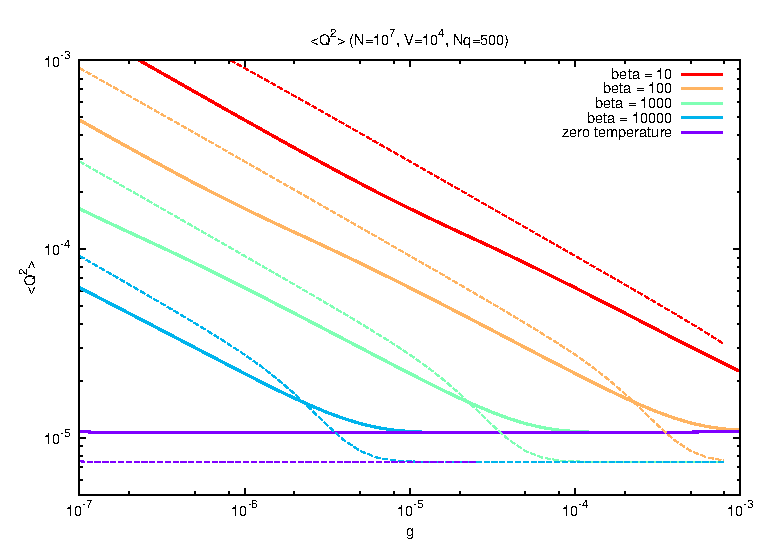
\includegraphics[width = 10cm]{./EPS/Q2.eps}
  \label{Q2}
\end{figure}
\begin{figure}[htbp]
  \centering
  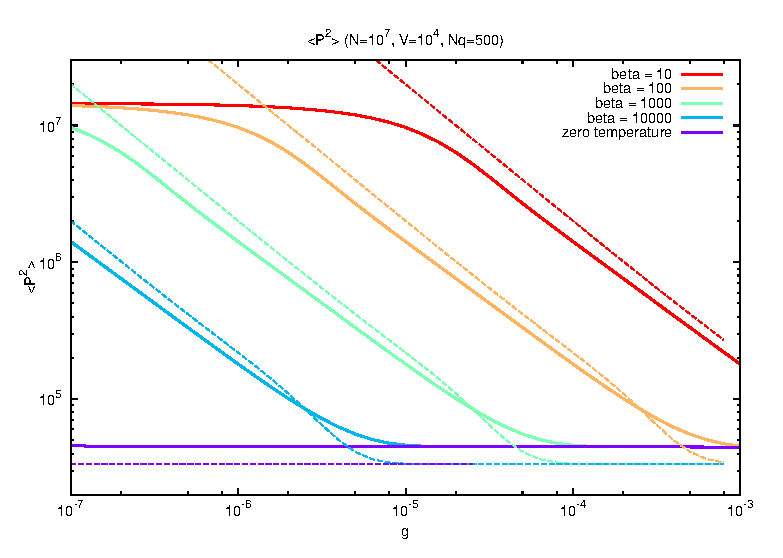
\includegraphics[width = 10cm]{./EPS/P2.eps}
  \label{P2}
\end{figure}
\\\\\\\\\\\\
図\ref{Q2},\ref{P2}\ :\ 破線は各温度に対する変分法による計算結果のプロット.$\ev{Q^2},\ev{P^2}$共に冪についてはよく一致している.

高温領域で位相ゆらぎ$\Delta Q = \sqrt{\ev{Q^2}}$,凝縮粒子数ゆらぎ$\Delta P = \sqrt{\ev{P^2}}$が増加する振る舞いは直感と一致している.
\newpage
\chapter{研究 : ゼロモードの緩和}
凝縮相と非凝縮相のcoupleを考え, 非平衡的な取り扱いを実現したい. 核生成のお話と関係がある. 位相の緩和とか見れるんじゃないかと期待. 
\section{公式}
QuantumMaster e.q.
\begin{eqnarray}
  i\dv{t}\rho_a^{nm}(t) = \sum_{n'm'}\bqty{\sum_{\mu\nu}\pqty{E_\mu - E_\nu}\Psi_{n}^{*, \mu}\Psi_{m}^{*, \nu}\Psi_{n'}^{\mu}\Psi_{m'}^{\nu}\rho_a^{n'm'}(t) + i\dpbra{nm}\hat{\calK}(t)\dpket{n'm'}\rho_a^{n'm'}(t)}
\end{eqnarray}
$A$をゼロモード演算子を含む項とする:
\begin{eqnarray}
  \dpbra{nm}A\dpket{n'm'} &=& A^{nn'}\delta_{mm'}\\
  \dpbra{nm}A^\dagger\dpket{n'm'} &=& A^{*, n'n}\delta_{mm'}\\
  \dpbra{nm}\tilde{A}\dpket{n'm'} &=& A^{*, mm'}\delta_{nn'}\\
  \dpbra{nm}\tilde{A^\dagger}\dpket{n'm'} &=& A^{m'm}\delta_{nn'}\\
\end{eqnarray}
プライム(')がつく位置に注意. これより
\begin{eqnarray}
  \dpbra{nm}\hat{A}\dpket{n'm'} &=& A^{nn'}\delta_{mm'} - A^{m'm}\delta_{nn'}\\
  \dpbra{nm}\hat{A^\dagger}\dpket{n'm'} &=& A^{*, n'n}\delta_{mm'} - A^{*, mm'}\delta_{nn'}
\end{eqnarray}
\section{具体計算 : time-convolutionless型}
もともと$\hat{\calK}(t, s),\ \dket{\rho_a(t)}$は相互作用描像のもとで定義されていたのをSchr\"odinger描像に移して計算. $s$の時間成分がexponentialの形で残ることになる.
\begin{eqnarray}
  \nonumber &&\dpbra{nm}\hat{A}_ie^{-i\hat{H}_a(t-s)}A_j^\dagger e^{i\hat{H}_a(t-s)}\dpket{n'm'}\\
  &=& \sum_{\mu\nu}\sum_{\mu'\nu'}\dpbra{nm}\hat{A}_i\dket{\mu\nu}e^{-i(E_\mu - E_\nu)(t-s)}\dbra{\mu\nu}A_j^\dagger \dket{\mu'\nu'}e^{i(E_{\mu'} - E_{\nu'})(t-s)}\dbra{\mu'\nu'}\dpket{nm}\\
  \nonumber &=& \sum_{n''m''}\sum_{\mu\nu}\sum_{\mu'\nu'}\bqty{A_i^{nn''}\delta_{mm''} - A_i^{m''m}\delta_{nn''}}A_j^{*, \mu'\mu}\delta_{\nu\nu'}\Psi_{n''}^{\mu}\Psi_{m''}^{\nu}\Psi_{n'}^{*, \mu'}\Psi_{m'}^{*, \nu'}e^{-i(E_\mu - E_\nu)(t-s)}e^{i(E_{\mu'} - E_{\nu'})(t-s)}\\
  \nonumber &=&\sum_{n''m''}\sum_{\mu\nu}\sum_{\mu'\nu'}A_i^{nn''}\delta_{mm''}A_j^{*, \mu'\mu}\delta_{\nu\nu'}\Psi_{n''}^{\mu}\Psi_{m''}^{\nu}\Psi_{n'}^{*, \mu'}\Psi_{m'}^{*, \nu'}e^{-i(E_\mu - E_\nu)(t-s)}e^{i(E_{\mu'} - E_{\nu'})(t-s)}\\
  &&- \sum_{n''m''}\sum_{\mu\nu}\sum_{\mu'\nu'}A_i^{m''m}\delta_{nn''}A_j^{*, \mu'\mu}\delta_{\nu\nu'}\Psi_{n''}^{\mu}\Psi_{m''}^{\nu}\Psi_{n'}^{*, \mu'}\Psi_{m'}^{*, \nu'}e^{-i(E_\mu - E_\nu)(t-s)}e^{i(E_{\mu'} - E_{\nu'})(t-s)}\\
  \nonumber &=&\sum_{n''}\sum_{\mu\nu}\sum_{\mu'}A_i^{nn''}A_j^{*, \mu'\mu}\Psi_{n''}^{\mu}\Psi_{m}^{\nu}\Psi_{n'}^{*, \mu'}\Psi_{m'}^{*, \nu}e^{-i(E_\mu - E_{\mu'})(t-s)}\\
  &&- \sum_{m''}\sum_{\mu\nu}\sum_{\mu'}A_i^{m''m}A_j^{*, \mu'\mu}\Psi_{n}^{\mu}\Psi_{m''}^{\nu}\Psi_{n'}^{*, \mu'}\Psi_{m'}^{*, \nu}e^{-i(E_\mu - E_{\mu'})(t-s)}\label{mid}
\end{eqnarray}
ここで$A_j^{*,\mu'\mu} = \sum_{nm}A^{*, mn}_n\Psi_n^{*, \mu}\Psi_m^{\mu'},\ \ \sum_\alpha \Psi_\beta^{*, \alpha}\Psi_{\beta'}^\alpha = \delta_{\beta\beta'}$であることを用いる:
\begin{eqnarray}
  \nonumber(\ref{mid}) &=&\sum_{n''}\sum_{\mu}\sum_{\mu'}A_i^{nn''}A_j^{*, \mu'\mu}\Psi_{n''}^{\mu}\Psi_{n'}^{*, \mu'}\delta_{mm'}e^{-i(E_\mu - E_{\mu'})(t-s)}\\
  &&- \sum_{m''}\sum_{\mu}\sum_{\mu'}A_i^{m''m}A_j^{*, \mu'\mu}\Psi_{n}^{\mu}\Psi_{n'}^{*, \mu'}\delta_{m'm''}e^{-i(E_\mu - E_{\mu'})(t-s)}\\
  \nonumber &=&\sum_{n''}\sum_{\mu}\sum_{\mu'}A_i^{nn''}A_j^{*, \mu'\mu}\Psi_{n''}^{\mu}\Psi_{n'}^{*, \mu'}\delta_{mm'}e^{-i(E_\mu - E_{\mu'})(t-s)}\\
  &&- \sum_{\mu}\sum_{\mu'}A_i^{m'm}A_j^{*, \mu'\mu}\Psi_{n}^{\mu}\Psi_{n'}^{*, \mu'}e^{-i(E_\mu - E_{\mu'})(t-s)}\\
  \nonumber &=&\sum_{n'''m'''}\sum_{n''}\sum_{\mu}\sum_{\mu'}A_i^{nn''}A_j^{*, m'''n'''}\Psi_{n'''}^{*, \mu}\Psi_{m'''}^{\mu'}\Psi_{n''}^{\mu}\Psi_{n'}^{*, \mu'}\delta_{mm'}e^{-i(E_\mu - E_{\mu'})(t-s)}\\
  &&- \sum_{n'''m'''}\sum_{\mu}\sum_{\mu'}A_i^{m'm}A_j^{*, m'''n'''}\Psi_{n'''}^{*, \mu}\Psi_{m'''}^{\mu'}\Psi_{n}^{\mu}\Psi_{n'}^{*, \mu'}e^{-i(E_\mu - E_{\mu'})(t-s)}\\
  \nonumber &=&\sum_{n'''m'''}\sum_{\mu}\sum_{\mu'}\bqty{\sum_{n''}A_i^{nn''}A_j^{*, m'''n'''}\Psi_{n''}^{\mu}\delta_{mm'}- A_i^{m'm}A_j^{*, m'''n'''}\Psi_{n}^{\mu}}\Psi_{n'''}^{*, \mu}\Psi_{m'''}^{\mu'}\Psi_{n'}^{*, \mu'}e^{-i(E_\mu - E_{\mu'})(t-s)}\label{end1}\\
\end{eqnarray}
同様に$\hat{\calK}$に必要な項を計算していく.
\begin{comment}
  以下では(\ref{end1})と添字が異なる部分に下線を引いている.
\end{comment}
\begin{eqnarray}
  \nonumber &&\dpbra{nm}\hat{A^\dagger}_ie^{-i\hat{H}_a(t-s)}\tilde{A}_j^\dagger e^{i\hat{H}_a(t-s)}\dpket{n'm'}\\
  %&=& \sum_{\mu\nu}\sum_{\mu'\nu'}\dpbra{nm}\hat{A^\dagger}_i\dket{\mu\nu}e^{-i(E_\mu - E_\nu)(t-s)}\dbra{\mu\nu}\tilde{A}_j^\dagger \dket{\mu'\nu'}e^{i(E_{\mu'} - E_{\nu'})(t-s)}\dbra{\mu'\nu'}\dpket{nm}\\
  \nonumber &=& \sum_{n''m''}\sum_{\mu\nu}\sum_{\mu'\nu'}\bqty{A_i^{*,  {n''n}}\delta_{mm''} - A_i^{*,  {mm''}}\delta_{nn''}}A_j^{ {\nu'\nu}}\delta_{ {\mu\mu'}}\Psi_{n''}^{\mu}\Psi_{m''}^{\nu}\Psi_{n'}^{*, \mu'}\Psi_{m'}^{*, \nu'}e^{-i(E_\mu - E_\nu)(t-s)}e^{i(E_{\mu'} - E_{\nu'})(t-s)}\\
  \nonumber &=&\sum_{n''m''}\sum_{\mu\nu}\sum_{\mu'\nu'}A_i^{*,  {n''n}}\delta_{mm''}A_j^{ {\nu'\nu}}\delta_{ {\mu\mu'}}\Psi_{n''}^{\mu}\Psi_{m''}^{\nu}\Psi_{n'}^{*, \mu'}\Psi_{m'}^{*, \nu'}e^{-i(E_\mu - E_\nu)(t-s)}e^{i(E_{\mu'} - E_{\nu'})(t-s)}\\
  &&- \sum_{n''m''}\sum_{\mu\nu}\sum_{\mu'\nu'}A_i^{*,  {mm''}}\delta_{nn''}A_j^{ {\nu'\nu}}\delta_{ {\mu\mu'}}\Psi_{n''}^{\mu}\Psi_{m''}^{\nu}\Psi_{n'}^{*, \mu'}\Psi_{m'}^{*, \nu'}e^{-i(E_\mu - E_\nu)(t-s)}e^{i(E_{\mu'} - E_{\nu'})(t-s)}\\
  \nonumber &=&\sum_{n''}\sum_{\mu\nu}\sum_{ {\nu'}}A_i^{*,  {n''n}}A_j^{ {\nu'\nu}}\Psi_{n''}^{\mu}\Psi_{m}^{\nu}\Psi_{n'}^{*, \mu}\Psi_{m'}^{*, \nu'}e^{ {i(E_\nu- E_{\nu'})(t-s)}}\\
  &&- \sum_{m''}\sum_{\mu\nu}\sum_{ {\nu'}}A_i^{*,  {mm''}}A_j^{ {\nu'\nu}}\Psi_{n}^{\mu}\Psi_{m''}^{\nu}\Psi_{n'}^{*, \mu}\Psi_{m'}^{*, \nu'}e^{ {i(E_\nu- E_{\nu'})(t-s)}}\\
  %\nonumber &=&\sum_{n''}\sum_{ {\nu}}\sum_{ {\nu'}}A_i^{*,  {n''n}}A_j^{ {\nu'\nu}}\Psi_{m}^{\nu}\Psi_{m'}^{*, \nu'}\delta_{ {n'n''}}e^{ {i(E_\nu- E_{\nu'})(t-s)}}\\
  %&&- \sum_{m''}\sum_{ {\nu}}\sum_{ {\nu'}}A_i^{*,  {mm''}}A_j^{ {\nu'\nu}}\Psi_{m''}^{\nu}\Psi_{m'}^{*, \nu'}\delta_{ {nn'}}e^{ {i(E_\nu- E_{\nu'})(t-s)}}\\
  \nonumber &=&\sum_{ {\nu}}\sum_{ {\nu'}}A_i^{*,  {n'n}}A_j^{ {\nu'\nu}}\Psi_{m}^{\nu}\Psi_{m'}^{*, \nu'}e^{ {i(E_\nu- E_{\nu'})(t-s)}}\\
  &&- \sum_{ {m''}}\sum_{ {\nu}}\sum_{ {\nu'}}A_i^{*,  {mm''}}A_j^{ {\nu'\nu}}\Psi_{m''}^{\nu}\Psi_{m'}^{*, \nu'}\delta_{ {nn'}}e^{ {i(E_\nu- E_{\nu'})(t-s)}}\\
  \nonumber &=&\sum_{n'''m'''}\sum_{ {\nu}}\sum_{ {\nu'}}A_i^{*, {n'n}}A_j^{{n'''m'''}}\Psi_{n'''}^{ {*, \nu'}}\Psi_{m'''}^{ {\nu}}\Psi_{m}^{ {\nu}}\Psi_{m'}^{*, \nu'}e^{ {i(E_\nu- E_{\nu'})(t-s)}}\\
  &&- \sum_{n'''m'''}\sum_{ {m''}}\sum_{ {\nu}}\sum_{ {\nu'}}A_i^{*,  {mm''}}A_j^{ {n'''m'''}}\Psi_{n'''}^{ {*, \nu'}}\Psi_{m'''}^{ {\nu}}\Psi_{m''}^{\nu}\Psi_{m'}^{*, \nu'}\delta_{ {nn'}}e^{ {i(E_\nu- E_{\nu'})(t-s)}}\\
  \nonumber &=&\sum_{n'''m'''}\sum_{\nu}\sum_{\nu'}\bqty{A_i^{*, n'n}A_j^{n'''m'''}\Psi_{m}^{\nu} - \sum_{m''}A_i^{*, mm''}A_j^{n'''m'''}\Psi_{m''}^{\nu}\delta_{nn'}}\Psi_{n'''}^{*, \nu'}\Psi_{m'''}^{\nu}\Psi_{m'}^{*, \nu'}e^{i(E_\nu- E_{\nu'})(t-s)}\\
\end{eqnarray}

\begin{eqnarray}
  \nonumber  &&\dpbra{nm}\hat{A}_ie^{-i\hat{H}_a(t-s)}\tilde{A}_j e^{i\hat{H}_a(t-s)}\dpket{n'm'}\\
  \nonumber &=& \sum_{n''m''}\sum_{\mu\nu}\sum_{\mu'\nu'}\bqty{A_i^{ {nn''}}\delta_{mm''} - A_i^{ {m''m}}\delta_{nn''}}A_j^{ {*, \nu'\nu}}\delta_{ {\mu\mu'}}\Psi_{n''}^{\mu}\Psi_{m''}^{\nu}\Psi_{n'}^{*, \mu'}\Psi_{m'}^{*, \nu'}e^{-i(E_\mu - E_\nu)(t-s)}e^{i(E_{\mu'} - E_{\nu'})(t-s)}\\
  \nonumber &=&\sum_{n''}\sum_{\mu\nu}\sum_{ {\nu'}}A_i^{nn''}A_j^{*, \nu'\nu}\Psi_{n''}^{\mu}\Psi_{m}^{\nu}\Psi_{n'}^{*, \mu}\Psi_{m'}^{*, \nu'}e^{ {i(E_\nu- E_{\nu'})(t-s)}}\\
  &&- \sum_{m''}\sum_{\mu\nu}\sum_{ {\nu'}}A_i^{m''m}A_j^{ {*, \nu'\nu}}\Psi_{n}^{\mu}\Psi_{m''}^{\nu}\Psi_{n'}^{*, \mu}\Psi_{m'}^{*, \nu'}e^{ {i(E_\nu- E_{\nu'})(t-s)}}\\
  \nonumber &=&\sum_{n''}\sum_{ {\nu}}\sum_{ {\nu'}}A_i^{ {nn''}}A_j^{*, \nu'\nu}\Psi_{m}^{\nu}\Psi_{m'}^{*, \nu'}\delta_{ {n'n''}}e^{ {i(E_\nu- E_{\nu'})(t-s)}}\\
  &&- \sum_{m''}\sum_{ {\nu}}\sum_{ {\nu'}}A_i^{m''m}A_j^{*, \nu'\nu}\Psi_{m''}^{\nu}\Psi_{m'}^{*, \nu'}\delta_{ {nn'}}e^{ {i(E_\nu- E_{\nu'})(t-s)}}\\
  %  \nonumber &=&\sum_{ {\nu}}\sum_{ {\nu'}}A_i^{nn'}A_j^{*, \nu'\nu}\Psi_{m}^{\nu}\Psi_{m'}^{*, \nu'}e^{ {i(E_\nu- E_{\nu'})(t-s)}}\\
  % &&- \sum_{ {m''}}\sum_{ {\nu}}\sum_{ {\nu'}}A_i^{m''m}A_j^{*, \nu'\nu}\Psi_{m''}^{\nu}\Psi_{m'}^{*, \nu'}\delta_{ {nn'}}e^{ {i(E_\nu- E_{\nu'})(t-s)}}\\
  \nonumber &=&\sum_{n'''m'''}\sum_{ {\nu}}\sum_{ {\nu'}}A_i^{nn'}A_j^{*, m'''n'''}\Psi_{n'''}^{ {*, \nu'}}\Psi_{m'''}^{ {\nu}}\Psi_{m}^{ {\nu}}\Psi_{m'}^{*, \nu'}e^{ {i(E_\nu- E_{\nu'})(t-s)}}\\
  &&- \sum_{n'''m'''}\sum_{ {m''}}\sum_{ {\nu}}\sum_{ {\nu'}}A_i^{m''m}A_j^{*, m'''n'''}\Psi_{n'''}^{ {*, \nu'}}\Psi_{m'''}^{ {\nu}}\Psi_{m''}^{\nu}\Psi_{m'}^{*, \nu'}\delta_{ {nn'}}e^{ {i(E_\nu- E_{\nu'})(t-s)}}\\
  \nonumber &=&\sum_{n'''m'''}\sum_{\nu}\sum_{\nu'}\bqty{A_i^{nn'}A_j^{*, m'''n'''}\Psi_{m}^{\nu}- \sum_{m''}A_i^{m''m}A_j^{*, m'''n'''}\Psi_{m''}^{\nu}\delta_{nn'} }\Psi_{n'''}^{*, \nu'}\Psi_{m'''}^{\nu}\Psi_{m'}^{*, \nu'}e^{i(E_\nu- E_{\nu'})(t-s)}\\
\end{eqnarray}
\begin{eqnarray}
  \nonumber  &&\dpbra{nm}\hat{A^\dagger}_ie^{-i\hat{H}_a(t-s)}A_j e^{i\hat{H}_a(t-s)}\dpket{n'm'}\\
  \nonumber &=& \sum_{n''m''}\sum_{\mu\nu}\sum_{\mu'\nu'}\bqty{A_i^{*, n''n}\delta_{mm''} - A_i^{*, mm''}\delta_{nn''}}A_j^{ {\mu\mu'}}\delta_{ {\nu\nu'}}\Psi_{n''}^{\mu}\Psi_{m''}^{\nu}\Psi_{n'}^{*, \mu'}\Psi_{m'}^{*, \nu'}e^{-i(E_\mu - E_\nu)(t-s)}e^{i(E_{\mu'} - E_{\nu'})(t-s)}\\
  \nonumber &=&\sum_{n''}\sum_{\mu\nu}\sum_{ {\mu'}}A_i^{*, n''n}A_j^{\mu\mu'}\Psi_{n''}^{\mu}\Psi_{m}^{\nu}\Psi_{n'}^{*, \mu'}\Psi_{m'}^{*, \nu}e^{ {-i(E_\mu- E_{\mu'})(t-s)}}\\
  &&- \sum_{m''}\sum_{\mu\nu}\sum_{ {\mu'}}A_i^{*, mm''}A_j^{\mu\mu'}\Psi_{n}^{\mu}\Psi_{m''}^{\nu}\Psi_{n'}^{*, \mu'}\Psi_{m'}^{*, \nu}e^{ {-i(E_\mu- E_{\mu'})(t-s)}}\\
  \nonumber &=&\sum_{n''}\sum_{ {\mu}}\sum_{ {\mu'}}A_i^{ {*, n''n}}A_j^{\mu\mu'}\Psi_{n''}^{\mu}\Psi_{n'}^{*, \mu'}\delta_{mm'}e^{ {-i(E_\mu- E_{\mu'})(t-s)}}\\
  &&- \sum_{m''}\sum_{ {\mu}}\sum_{ {\mu'}}A_i^{*, mm''}A_j^{\mu\mu'}\Psi_{n}^{\mu}\Psi_{n'}^{*, \mu'}\delta_{m'm''}e^{ {-i(E_\mu- E_{\mu'})(t-s)}}\\
  \nonumber &=&\sum_{n'''m'''}\sum_{n''}\sum_{ {\mu}}\sum_{ {\mu'}}A_i^{ {*, n''n}}A_j^{n'''m'''}\Psi_{n'''}^{*, \mu}\Psi_{m'''}^{\mu'}\Psi_{n''}^{\mu}\Psi_{n'}^{*, \mu'}\delta_{mm'}e^{ {-i(E_\mu- E_{\mu'})(t-s)}}\\
  &&- \sum_{n'''m'''}\sum_{ {\mu}}\sum_{ {\mu'}}A_i^{*, mm'}A_j^{n'''m'''}\Psi_{n'''}^{*, \mu}\Psi_{m'''}^{\mu'}\Psi_{n}^{\mu}\Psi_{n'}^{*, \mu'}e^{ {-i(E_\mu- E_{\mu'})(t-s)}}\\
  \nonumber &=&\sum_{n'''m'''}\sum_{ {\mu}}\sum_{ {\mu'}}\bqty{\sum_{n''}A_i^{ {*, n''n}}A_j^{n'''m'''}\Psi_{n''}^{\mu}\delta_{mm'} - A_i^{*, mm'}A_j^{n'''m'''}\Psi_{n}^{\mu}}\Psi_{n'''}^{*, \mu}\Psi_{m'''}^{\mu'}\Psi_{n'}^{*, \mu'}e^{ {-i(E_\mu- E_{\mu'})(t-s)}}\\
\end{eqnarray}
まとめると,
\begin{screen}
  \begin{eqnarray}
    \nonumber    &&\dpbra{nm}\hat{A}_ie^{-i\hat{H}_a(t-s)}A_j^\dagger e^{i\hat{H}_a(t-s)}\dpket{n'm'}\\
    \nonumber    &=&\sum_{n'''m'''}\sum_{\mu}\sum_{\mu'}\bqty{\sum_{n''}A_i^{nn''}A_j^{*, m'''n'''}\Psi_{n''}^{\mu}\delta_{mm'}- A_i^{m'm}A_j^{*, m'''n'''}\Psi_{n}^{\mu}}\Psi_{n'''}^{*, \mu}\Psi_{m'''}^{\mu'}\Psi_{n'}^{*, \mu'}e^{-i(E_\mu - E_{\mu'})(t-s)}\\\\
    \nonumber &&\dpbra{nm}\hat{A^\dagger}_ie^{-i\hat{H}_a(t-s)}\tilde{A}_j^\dagger e^{i\hat{H}_a(t-s)}\dpket{n'm'}\\
    \nonumber    &=&\sum_{n'''m'''}\sum_{\nu}\sum_{\nu'}\bqty{A_i^{*, n'n}A_j^{n'''m'''}\Psi_{m}^{\nu}- \sum_{m''}A_i^{*, mm''}A_j^{n'''m'''}\Psi_{m''}^{\nu}\delta_{nn'}}\Psi_{n'''}^{*, \nu'}\Psi_{m'''}^{\nu}\Psi_{m'}^{*, \nu'}e^{i(E_\nu- E_{\nu'})(t-s)}\\\\
    \nonumber&&\dpbra{nm}\hat{A}_ie^{-i\hat{H}_a(t-s)}\tilde{A}_j e^{i\hat{H}_a(t-s)}\dpket{n'm'}\\
    \nonumber    &=&\sum_{n'''m'''}\sum_{\nu}\sum_{\nu'}\bqty{A_i^{nn'}A_j^{*, m'''n'''}\Psi_{m}^{\nu}- \sum_{m''}A_i^{m''m}A_j^{*, m'''n'''}\Psi_{m''}^{\nu}\delta_{nn'} }\Psi_{n'''}^{*, \nu'}\Psi_{m'''}^{\nu}\Psi_{m'}^{*, \nu'}e^{i(E_\nu- E_{\nu'})(t-s)}\\\\
    \nonumber    &&\dpbra{nm}\hat{A^\dagger}_ie^{-i\hat{H}_a(t-s)}A_j e^{i\hat{H}_a(t-s)}\dpket{n'm'}\\
    \nonumber &=&\sum_{n'''m'''}\sum_{ {\mu}}\sum_{ {\mu'}}\bqty{\sum_{n''}A_i^{ {*, n''n}}A_j^{n'''m'''}\Psi_{n''}^{\mu}\delta_{mm'} - A_i^{*, mm'}A_j^{n'''m'''}\Psi_{n}^{\mu}}\Psi_{n'''}^{*, \mu}\Psi_{m'''}^{\mu'}\Psi_{n'}^{*, \mu'}e^{ {-i(E_\mu- E_{\mu'})(t-s)}}\\
  \end{eqnarray}
\end{screen}
\textbf{添字が合ってるかとっても心配.}

\section{具体計算 : 摂動項$\calK(t)$}
我々が計算したいのは
\begin{eqnarray}
  \calK(t) &=& \calK_1(t) + \calK_2(t)\\
  \nonumber  \calK_1(t)&=& -\frac{2Vg^2}{(2\pi)^6}\int_{t_0}^tds\int d\bm{k}_1d\bm{k}_2d\bm{k}_3\delta(\bm{k}_1+\bm{k}_2-\bm{k}_3)\\
  \nonumber  &&\times\Bigl[n_{k_1}n_{k_2}(1+n_{k_3})\Bqty{ e^{i(\omega_{k_1}+\omega_{k_2}  - \omega_{k_3})(t-s)}\hat{A}_1(t)A_1^\dagger(s) - e^{-i(\omega_{k_1}+\omega_{k_2}  - \omega_{k_3})(t-s)}\hat{A}^\dagger_1(t)\tilde{A}_1^\dagger(s) }\\
    \nonumber  &&-(1+n_{k_1})(1+n_{k_2})n_{k_3}\Bqty{e^{i(\omega_{k_1}+\omega_{k_2}  - \omega_{k_3})(t-s)}\hat{A}_1(t)\tilde{A}_1(s) - e^{-i(\omega_{k_1}+\omega_{k_2}  - \omega_{k_3})(t-s)}\hat{A}^\dagger_1(t)A_1(s) }\Bigr]\\
  \\
  \nonumber  \calK_2(t) &=& -\frac{Vg^2}{2(2\pi)^6}\int_{t_0}^tds\int d\bm{k}\Bigl[ n_k^2\Bqty{e^{2i\omega_{k}(t-s)}\hat{A}_2(t)A_2^\dagger(s) - e^{-2i\omega_{k}(t-s)}\hat{A}^\dagger_2(t)\tilde{A}_2^\dagger(s)}\\
    &&-(1+n_{k})^2\Bqty{e^{2i\omega_{k}(t-s)}\hat{A}_2(t)\tilde{A}_2(s) - e^{-2i\omega_{k}(t-s)}\hat{A}^\dagger_2(t)A_2(s)}\Bigr]
\end{eqnarray}
だが, 演算子は全て相互作用描像である. これをSchr\"odinger描像に移して計算するので, $A(s)\rightarrow e^{-i\hat{H}_a(t-s)}Ae^{i\hat{H}_a(t-s)}$として期待値を取る. Schr\"odinger描像に移した期待値の公式は既に上で導出した.

さらにQuantum Master e.q.をマルコフ近似すると$\dket{\rho_a(s)}\rightarrow\dket{\rho_a(t)}$かつ$t_0\rightarrow -\infty$とすればよい. $s$積分は
\begin{eqnarray}
  \int_{-\infty}^t ds e^{iW(t-s)} \simeq \pi\delta(W)
\end{eqnarray}
\underline{のように計算できる(主値を捨てている)}ことから, $\dpbra{nm}\calK_2(t)\dpket{n'm'}$は
\begin{eqnarray}
  &&\dpbra{nm}\calK_2(t)\dpket{n'm'} = -\frac{Vg^2}{2(2\pi)^6}\int d\bm{k}\\
  \nonumber  &&\times\sum_{n'''m'''}\Bigl[ n_k^2\Bqty{\sum_{n''}A_2^{nn''}A_2^{*, m'''n'''}\delta_{mm'}M_{n'''n''}M_{n'm'''}' - A_2^{m'm}A_2^{*, m'''n'''}M_{n'''n}M_{n'm'''}'}\delta(2\omega_k - E_\mu + E_{\mu'})\\
    \nonumber &&\ \ + n_k^2\Bqty{A_2^{*, n'n}A_2^{n'''m'''}N_{mm'''}N_{n'''m'}' - \sum_{m''}A_2^{*, mm''}A_2^{n'''m'''}\delta_{nn'}N_{m''m'''}N_{n'''m'}'}\delta(-2\omega_k + E_\nu - E_{\nu'})\\
    \nonumber &&- (1 + n_k)^2\Bqty{A_2^{nn'}A_2^{*, m'''n'''}N_{mm'''}N_{n'''m'}' - \sum_{m''}A_2^{m''m}A_2^{*, m'''n'''}\delta_{nn'}N_{m''m'''}N_{n'''m'}'}\delta(2\omega_k + E_\nu - E_{\nu'})\\
    \nonumber&&-(1+n_k)^2\Bqty{\sum_{n''}A_2^{*, n''n}A_2^{n'''m'''}\delta_{mm'}M_{n'''n''}M_{n'm'''}' - A_2^{*, mm'}A_2^{n'''m'''}M_{n'''n}M_{n'm'''}'}\delta(-2\omega_k - E_\mu + E_{\mu'})\Bigr]\\
\end{eqnarray}
ここで
\begin{eqnarray}
  M_{\alpha\beta} &\equiv& \sum_\mu \Psi_\alpha^{*, \mu}\Psi_\beta^{\mu}\hspace{0.5cm}M_{\alpha\beta}' \equiv \sum_{\mu'} \Psi_\alpha^{*, \mu'}\Psi_\beta^{\mu'}\\
  N_{\alpha\beta} &\equiv& \sum_\nu \Psi_\alpha^{\nu}\Psi_\beta^{\nu}\hspace{0.5cm}N_{\alpha\beta}' \equiv \sum_{\nu'} \Psi_\alpha^{*, \nu'}\Psi_\beta^{*, \nu'}
\end{eqnarray}
としている. さらに$\bm{k}$積分を実行する. ここで
\begin{eqnarray}
  \int d\bm{k} n_k^2\delta(2\omega_k - E) &=& \int_0^\infty dk\int_0^\pi d\theta \int_0^{2\pi}d\phi k\sin{\theta}n_k^2\delta(k^2 - E) \\
  &=& \int_0^\pi d\theta \int_0^{2\pi}d\phi \sqrt{E}\theta(E)\sin{\theta}n_k^2\\
  &=& 4\pi\sqrt{E}\theta(E)n_E^2
\end{eqnarray}
であることから
\begin{eqnarray}
  R_2(E) \equiv \frac{Vg^2}{8\pi}\theta(E)n_E^2\sqrt{E}\hspace{0.5cm}R_2'(E) \equiv \frac{Vg^2}{8\pi}\theta(E)(1 + n_E)^2\sqrt{E}
\end{eqnarray}
とする. スターの位置に注意. ここで$\theta(E)$は階段関数. これを用いると
\begin{eqnarray}
  \nonumber &&\dpbra{nm}\calK_2(t)\dpket{n'm'} =\\
  \nonumber &&\sum_{n'''m'''}\Bigl[-\Bqty{\sum_{n''}A_2^{nn''}A_2^{*, m'''n'''}\delta_{mm'}M_{n'''n''}M_{n'm'''}' - A_2^{m'm}A_2^{*, m'''n'''}M_{n'''n}M_{n'm'''}'}R_2(E_\mu - E_{\mu'})\\
    \nonumber &&- \Bqty{A_2^{*, n'n}A_2^{n'''m'''}N_{mm'''}N_{n'''m'}' - \sum_{m''}A_2^{*, mm''}A_2^{n'''m'''}\delta_{nn'}N_{m''m'''}N_{n'''m'}'}R_2(E_\nu - E_{\nu'})\\
    \nonumber &&+ \Bqty{A_2^{nn'}A_2^{*, m'''n'''}N_{mm'''}N_{n'''m'}' - \sum_{m''}A_2^{m''m}A_2^{*, m'''n'''}\delta_{nn'}N_{m''m'''}N_{n'''m'}'}R_2'(-E_\nu + E_{\nu'})\\
    \nonumber&&+\Bqty{\sum_{n''}A_2^{*, n''n}A_2^{n'''m'''}\delta_{mm'}M_{n'''n''}M_{n'm'''}' - A_2^{*, mm'}A_2^{n'''m'''}M_{n'''n}M_{n'm'''}'}R_2'(- E_\mu + E_{\mu'})\Bigr]\\\label{K1}
\end{eqnarray}
\textbf{符号が合ってるかどうかとても心配.}

さらに$\dpbra{nm}\calK_1(t)\dpket{n'm'}$を計算する前に\underline{積分公式を導出しておく}:
\begin{eqnarray}
  I(E) &=& \int d\bm{k}_1d\bm{k}_2d\bm{k}_3\delta(\bm{k}_1+\bm{k}_2-\bm{k}_3)\delta(\omega_{k_1} + \omega_{k_2} - \omega_{k_3} + E)a(\omega_{k_1})b(\omega_{k_2})c(\omega_{k_3})\\
  &=& 8\pi^2\int_0^\infty d\omega_1\int_{\frac{E_2}{4\omega_1}}^\infty d\omega_2 a(\omega_1)b(\omega_2)c(\omega_1 + \omega_2 + E)
\end{eqnarray}
となる. これ以上は$a, b, c$の具体形が必要. これを用いると(\ref{K1})の添字を$2\rightarrow1$にしたものと同様. ただし:
\begin{eqnarray}
  R_1(E) &=& \frac{Vg^2}{4\pi^3}\int_0^\infty d\omega_1\int_{\frac{E^2}{4\omega_1}}^\infty d\omega_2 n_{\omega_1}n_{\omega_2}(1 + n_{\omega_1 + \omega_2 + E})\\
  R_1'(E) &=& \frac{Vg^2}{4\pi^3}\int_0^\infty d\omega_1\int_{\frac{E^2}{4\omega_1}}^\infty d\omega_2 (1 + n_{\omega_1})(1 + n_{\omega_2})n_{\omega_1 + \omega_2 + E}
\end{eqnarray}
とする. つまり解くべき方程式は
\begin{eqnarray}
  i\dv{t}\rho_a^{nm}(t) &=& \sum_{n'm'}\bqty{\sum_{\mu\nu}\pqty{E_\mu - E_\nu}\Psi_{n}^{*, \mu}\Psi_{m}^{*, \nu}\Psi_{n'}^{\mu}\Psi_{m'}^{\nu} + i\dpbra{nm}\hat{\calK}(t)\dpket{n'm'}}\rho_a^{n'm'}(t)\\
  &\equiv& \sum_{n'm'} L^{nm, n'm'}\rho_a^{n'm'}(t)\label{Master2}
\end{eqnarray}
である. ただし
\begin{eqnarray}
  &&L^{nm, n'm'} = \sum_{\mu\nu}\pqty{E_\mu - E_\nu}\Psi_{n}^{*, \mu}\Psi_{m}^{*, \nu}\Psi_{n'}^{\mu}\Psi_{m'}^{\nu} \\
  &&+\sum_{i = 1, 2}\sum_{n'''m'''}\Bigl[\nonumber -\Bqty{\sum_{n''}A_i^{nn''}A_i^{*, m'''n'''}\delta_{mm'}M_{n'''n''}M_{n'm'''}' - A_i^{m'm}A_i^{*, m'''n'''}M_{n'''n}M_{n'm'''}'}R_i(E_\mu - E_{\mu'})\\
    \nonumber &&- \Bqty{A_i^{*, n'n}A_i^{n'''m'''}N_{mm'''}N_{n'''m'}' - \sum_{m''}A_i^{*, mm''}A_i^{n'''m'''}\delta_{nn'}N_{m''m'''}N_{n'''m'}'}R_i(E_\nu - E_{\nu'})\\
    \nonumber &&+ \Bqty{A_i^{nn'}A_i^{*, m'''n'''}N_{mm'''}N_{n'''m'}' - \sum_{m''}A_i^{m''m}A_i^{*, m'''n'''}\delta_{nn'}N_{m''m'''}N_{n'''m'}'}R_i'(-E_\nu + E_{\nu'})\\
    \nonumber&&+\Bqty{\sum_{n''}A_i^{*, n''n}A_i^{n'''m'''}\delta_{mm'}M_{n'''n''}M_{n'm'''}' - A_i^{*, mm'}A_i^{n'''m'''}M_{n'''n}M_{n'm'''}'}R_i'(- E_\mu + E_{\mu'})\Bigr]\\\label{L}
\end{eqnarray}
\section{数値計算へ向けて}
期待値の計算のためにQuantum Master e.q.(\ref{Master2})を解いて密度行列$\rho_a$を得るのがひとまずの目的. これが得られればいろんな物理量の計算ができる. (\ref{Master2})のエッセンスは$L^{nm, n'm'}$にある. $L^{nm, n'm'}$を数値計算においてどのように表現するかをまとめる.
\subsection{$E_\mu\cdot E_\nu$}
$\ket{\mu},\ \ket{\nu}$は$H_a$のエネルギー固有状態として定義されている:
\begin{eqnarray}
  H_a\ket{\mu} = E_\mu\ket{\mu},\hspace{0.5cm}\tilde{H}_a\ket{\nu} = E_\nu\ket{\nu}
\end{eqnarray}
$\ket{\nu}$はチルダハミルトニアンの固有状態というだけで, 実質ノンチルダとモノに変わりはない. ということで, これを$\varphi_{\rm ex},\ \varphi_{\rm ex}^\dagger$の粒子数状態で行列表示する:
\begin{eqnarray}
  \sum_m\pbra{n}H_a\pket{m}(m\ket{\mu} &=& E_\mu(n\ket{\mu}\\
  \Longleftrightarrow  \sum_m\pbra{n}H_a\pket{m}\Psi_m^\mu &=& E_\mu\Psi_n^\mu
\end{eqnarray}
これをLapackで解けば$\Psi, E$のセットが得られる.
\subsection{$A_i^{nm}$}
$i = 1, 2$のみなので具体的に計算してみる:
\begin{eqnarray}
  A_1^{nm} &=& \pbra{n}A_1\pket{m} = \pbra{n}\varphi_0\pket{m} = \sqrt{m}(n|m-1) = \sqrt{m}\delta_{n, m-1}\\
  A_2^{nm} &=& \pbra{n}A_2\pket{m} = \pbra{n}\varphi_0^2\pket{m} = \sqrt{m(m-1)}(n|m-2) = \sqrt{m(m-1)}\delta_{n, m-2}\\
  A_2^{*, nm} &=& \pqty{A_2^{nm}}^* = A_2^{nm}
\end{eqnarray}
とても簡単になる.
\subsection{$N_{nm}\cdot N_{nm}'$}
\begin{eqnarray}
  N_{nm} = \sum_\nu\Psi_n^\nu\Psi_m^\nu
\end{eqnarray}
なので$\Psi$のセットがあれば自明.
\subsection{$R_i$}
$R_1, R_2$共に$n_k$が必要. $n_k$の定義は
\begin{eqnarray}
  n_k\delta(\bm{k} - \bm{k}') = \ev{b_{\bm{k}}b_{\bm{k}}^\dagger}
\end{eqnarray}
であり, $H_R$は$\varphi_{\rm ex}$の2次なので対角化可能. 系の時間発展に対して変化が少ない過程をしているので熱平衡状態にあると考えて良い:
\begin{eqnarray}
  n_k = \frac{1}{e^{\beta\omega_k'}-1}\delta(\bm{k} - \bm{k}')
\end{eqnarray}
一様系では
\begin{eqnarray}
  \omega_k' = \sqrt{\frac{\hbar^2k^2}{2m}\pqty{\frac{\hbar^2k^2}{2m} + 2gn_0}}
\end{eqnarray}
であることを利用して
\begin{eqnarray}
  && n_E = \frac{1}{e^{\beta\omega_E'}-1}\hspace{0.5cm}\omega_E' = \sqrt{\frac{\hbar^2E}{2m}\pqty{\frac{\hbar^2E}{2m} + 2gn_0}}\\
  &&n_{\omega_1 + \omega_2 + E} = \frac{1}{e^{\beta\omega'}-1}\hspace{0.5cm}\omega' = \sqrt{\frac{\hbar^2(\frac{\omega_1 + \omega_2}{2}+E)}{2m}\pqty{\frac{\hbar^2(\frac{\omega_1 + \omega_2}{2}+E)}{2m} + 2gn_0}}
\end{eqnarray}
とすることができる. また$\xi^2 = n_0$より$n_0$はTDGP方程式により決定される. つまり, $\xi$の時間発展は密度行列の時間発展とは別の枠組みで与えられていることになる. TDGPに量子補正を加えるべきかどうかはわからない. 量子補正を入れると自己無撞着の計算がとてもめんどくさくなる. 今のところ, ゼロモードはDepletionに影響を与えない(比熱は影響を受ける)という結論なので, 補正無しのTDGPでもよい気がする.

ちなみに今回は$\xi$は時間発展しないものとしているのであしからず. 
\section{$L^{nm,n'm'}$の整理}
以上の結論から$L^{nm,n'm'}$を整理する. (\ref{L})の第二項の和を$i = 1, 2$それぞれついて計算する.

i = 1について:
\begin{eqnarray}
  &&\sum_{n'''m'''}\Bigl[\nonumber -\Bqty{\sum_{n''}A_1^{nn''}A_1^{*, m'''n'''}\delta_{mm'}M_{n'''n''}M_{n'm'''}' - A_1^{m'm}A_1^{*, m'''n'''}M_{n'''n}M_{n'm'''}'}R_1(E_\mu - E_{\mu'})\\
    \nonumber &&- \Bqty{A_1^{*, n'n}A_1^{n'''m'''}N_{mm'''}N_{n'''m'}' - \sum_{m''}A_1^{*, mm''}A_1^{n'''m'''}\delta_{nn'}N_{m''m'''}N_{n'''m'}'}R_1(E_\nu - E_{\nu'})\\
    \nonumber &&+ \Bqty{A_1^{nn'}A_1^{*, m'''n'''}N_{mm'''}N_{n'''m'}' - \sum_{m''}A_1^{m''m}A_1^{*, m'''n'''}\delta_{nn'}N_{m''m'''}N_{n'''m'}'}R_1'(-E_\nu + E_{\nu'})\\
    \nonumber&&+\Bqty{\sum_{n''}A_1^{*, n''n}A_1^{n'''m'''}\delta_{mm'}M_{n'''n''}M_{n'm'''}' - A_1^{*, mm'}A_1^{n'''m'''}M_{n'''n}M_{n'm'''}'}R_1'(- E_\mu + E_{\mu'})\Bigr]\\
  \\
  &=&\sum_{n'''m'''}\Bigl[\nonumber -\Bqty{\sum_{n''}\sqrt{n''}\delta_{n, n''-1}\sqrt{n'''}\delta_{m''', n'''-1}\delta_{mm'}M_{n'''n''}M_{n'm'''}' - \sqrt{m}\delta_{m', m-1}\sqrt{n'''}\delta_{m''', n'''-1}M_{n'''n}M_{n'm'''}'}\\
    \nonumber&&\hspace{14cm}\times R_1(E_\mu - E_{\mu'})\\
    \nonumber &&- \Bqty{\sqrt{n}\delta_{n', n-1}\sqrt{m'''}\delta_{n''', m'''-1}N_{mm'''}N_{n'''m'}' - \sum_{m''}\sqrt{m''}\delta_{m, m''-1}\sqrt{m'''}\delta_{n''', m'''-1}\delta_{nn'}N_{m''m'''}N_{n'''m'}'}\\
    \nonumber&&\hspace{14cm}\times R_1(E_\nu - E_{\nu'})\\
    \nonumber &&+ \Bqty{\sqrt{n'}\delta_{n, n'-1}\sqrt{n'''}\delta_{m''', n'''-1}N_{mm'''}N_{n'''m'}' - \sum_{m''}\sqrt{m}\delta_{m'', m-1}\sqrt{n'''}\delta_{m''', n'''-1}\delta_{nn'}N_{m''m'''}N_{n'''m'}'}\\
    \nonumber&&\hspace{14cm}\times R_1'(-E_\nu + E_{\nu'})\\
    \nonumber&&+\Bqty{\sum_{n''}\sqrt{n}\delta_{n'', n-1}\sqrt{m'''}\delta_{n''', m'''-1}\delta_{mm'}M_{n'''n''}M_{n'm'''}' - \sqrt{m'}\delta_{m, m'-1}\sqrt{m'''}\delta_{n''', m'''-1}M_{n'''n}M_{n'm'''}'}\\
    \nonumber&&\hspace{14cm}\times R_1'(- E_\mu + E_{\mu'})\Bigr]\\
  \\
  &=&\sum_{\ell }\Bigl[\nonumber -\sum_{\mu\mu'}\Bqty{ \sqrt{n+1}\sqrt{\ell }\delta_{mm'}M_{\ell , n+1}M_{n', \ell -1}' -  \sqrt{m}\delta_{m', m-1}\sqrt{\ell }M_{\ell n}M_{n', \ell -1}'}R_1(E_\mu - E_{\mu'})\\
    \nonumber &&- \sum_{\nu\nu'}\Bqty{ \sqrt{n}\delta_{n', n-1}\sqrt{\ell +1}N_{m, \ell +1}N_{\ell m'}' -  \sqrt{m+1}\sqrt{\ell +1}\delta_{nn'}N_{m+1, \ell +1}N_{\ell m'}'}R_1(E_\nu - E_{\nu'})\\
    \nonumber &&+ \sum_{\nu\nu'}\Bqty{ \sqrt{n'}\delta_{n, n'-1}\sqrt{\ell }N_{m, \ell -1}N_{\ell m'}' -  \sqrt{m}\sqrt{\ell }\delta_{nn'}N_{m-1, \ell -1}N_{\ell m'}'}R_1'(-E_\nu + E_{\nu'})\\
    \nonumber&&+\sum_{\mu\mu'}\Bqty{ \sqrt{n}\sqrt{\ell +1}\delta_{mm'}M_{\ell , n-1}M_{n', \ell +1}' -  \sqrt{m'}\delta_{m, m'-1}\sqrt{\ell +1}M_{\ell n}M_{n'\ell +1}'}R_1'(- E_\mu + E_{\mu'})\Bigr]\\
\end{eqnarray}
$L^{nm, n'm'}$内の$n''m'', n'''m'''$和は$\ell$のみにまとまった. またここでは$MN, M'N'$に含まれていた$\mu\nu, \mu'\nu'$の和を露わに書き直した.

i = 2について:
\begin{eqnarray}
  &&\sum_{n'''m'''}\Bigl[\nonumber -\Bqty{\sum_{n''}A_2^{nn''}A_2^{*, m'''n'''}\delta_{mm'}M_{n'''n''}M_{n'm'''}' - A_2^{m'm}A_2^{*, m'''n'''}M_{n'''n}M_{n'm'''}'}R_2(E_\mu - E_{\mu'})\\
    \nonumber &&- \Bqty{A_2^{*, n'n}A_2^{n'''m'''}N_{mm'''}N_{n'''m'}' - \sum_{m''}A_2^{*, mm''}A_2^{n'''m'''}\delta_{nn'}N_{m''m'''}N_{n'''m'}'}R_2(E_\nu - E_{\nu'})\\
    \nonumber &&+ \Bqty{A_2^{nn'}A_2^{*, m'''n'''}N_{mm'''}N_{n'''m'}' - \sum_{m''}A_2^{m''m}A_2^{*, m'''n'''}\delta_{nn'}N_{m''m'''}N_{n'''m'}'}R_2'(-E_\nu + E_{\nu'})\\
    \nonumber&&+\Bqty{\sum_{n''}A_2^{*, n''n}A_2^{n'''m'''}\delta_{mm'}M_{n'''n''}M_{n'm'''}' - A_2^{*, mm'}A_2^{n'''m'''}M_{n'''n}M_{n'm'''}'}R_2'(- E_\mu + E_{\mu'})\Bigr]\\
  \\
  %&&\sum_{n'''m'''}\Bigl[\nonumber -\Bqty{\sum_{n''}\sqrt{n''(n''-1)}\delta_{n, n''-2}\sqrt{n'''(n'''-1)}\delta_{m''', n'''-2}\delta_{mm'}M_{n'''n''}M_{n'm'''}' - \sqrt{m(m-1)}\delta_{m', m-2}\sqrt{n'''(n'''-1)}\delta_{m''', n'''-2}M_{n'''n}M_{n'm'''}'}R_2(E_\mu - E_{\mu'})\\
  % \nonumber &&- \Bqty{\sqrt{n(n-1)}\delta_{n', n-2}\sqrt{m'''(m'''-1)}\delta_{n''', m'''-2}N_{mm'''}N_{n'''m'}' - \sum_{m''}\sqrt{m''(m''-1)}\delta_{m, m''-2}\sqrt{m'''(m'''-1)}\delta_{n''', m'''-2}\delta_{nn'}N_{m''m'''}N_{n'''m'}'}R_2(E_\nu - E_{\nu'})\\
  %\nonumber &&+ \Bqty{\sqrt{n'(n'-1)}\delta_{n, n'-2}\sqrt{n'''(n'''-1)}\delta_{m''', n'''-2}N_{mm'''}N_{n'''m'}' - \sum_{m''}\sqrt{m(m-1)}\delta_{m'', m-2}\sqrt{n'''(n'''-1)}\delta_{m''', n'''-2}\delta_{nn'}N_{m''m'''}N_{n'''m'}'}R_2'(-E_\nu + E_{\nu'})\\
  %\nonumber&&+\Bqty{\sum_{n''}\sqrt{n(n-1)}\delta_{n'', n-2}\sqrt{m'''(m'''-1)}\delta_{n''', m'''-2}\delta_{mm'}M_{n'''n''}M_{n'm'''}' - \sqrt{m'(m'-1)}\delta_{m, m'-2}\sqrt{m'''(m'''-1)}\delta_{n''', m'''-2}M_{n'''n}M_{n'm'''}'}R_2'(- E_\mu + E_{\mu'})\Bigr]\\
  %    \\
  &&\sum_{\ell }\Bigl[\nonumber -\sum_{\mu\mu'}\Bqty{\sqrt{(n+2)(n+1)}\sqrt{\ell (\ell -1)}\delta_{mm'}M_{\ell, n+2}M_{n', \ell -2}' - \sqrt{m(m-1)}\delta_{m', m-2}\sqrt{\ell (\ell -1)}M_{\ell, n}M_{n', \ell -2}'}\\
    \nonumber&&\hspace{14cm}\times R_2(E_\mu - E_{\mu'})\\
    \nonumber &&- \sum_{\nu\nu'}\Bqty{\sqrt{n(n-1)}\delta_{n', n-2}\sqrt{(\ell +2)(\ell +1)}N_{m, \ell +2}N_{\ell m'}' - \sqrt{(m+2)(m+1)}\sqrt{m'''(m'''-1)}\delta_{nn'}N_{m+2, \ell +2}N_{\ell m'}'}\\
    \nonumber&&\hspace{14cm}\times R_2(E_\nu - E_{\nu'})\\
    \nonumber &&+ \sum_{\nu\nu'}\Bqty{\sqrt{n'(n'-1)}\delta_{n, n'-2}\sqrt{\ell (\ell -1)}N_{m, \ell -2}N_{\ell m'}' - \sqrt{m(m-1)}\sqrt{\ell (\ell -1)}\delta_{nn'}N_{m-2, \ell -2}N_{\ell m'}'}\\
    \nonumber&&\hspace{14cm}\times R_2'(-E_\nu + E_{\nu'})\\
    \nonumber&&+\sum_{\mu\mu'}\Bqty{\sqrt{n(n-1)}\sqrt{(\ell +2)(\ell +1)}\delta_{mm'}M_{\ell , n-2}M_{n', \ell +2}' - \sqrt{m'(m'-1)}\delta_{m, m'-2}\sqrt{(\ell +2)(\ell +1)}M_{\ell n}M_{n', \ell +2}'}\\
    \nonumber&&\hspace{14cm}\times R_2'(- E_\mu + E_{\mu'})\Bigr]\\
\end{eqnarray}
$R_i$はシンプソン積分でいける.
\newpage
\chapter{研究 : BdG間及びZeromode-BdG間の相互作用を取り入れた有限温度系の計算}
熱力学ポテンシャルの摂動論については「高田康民 : 多体問題(朝倉書店, 1999)」を参考にしています.
\section{やりたいこと}
Y.Nakamura, T.Kawaguchi, Y.Torii, and Y.Yamanaka, arXiv:1604.05900v1(2016)の4章「Thermodynamical quantity and Partition Function」の式(43)では分配関数を
\begin{eqnarray}
  Z = Z_{\rm u, z}Z_{\rm u,ex}
\end{eqnarray}
として評価をしているが, これを
\begin{eqnarray}
  Z = Z_{\rm u, z}Z_{\rm u,ex}Z_{\rm \rm int}
\end{eqnarray}
として評価したい. $Z_{\rm \rm int}$にはゼロモード $\varphi_{z}$ とBdG $\varphi_{\rm ex}$ のカップリング項や$\varphi_{\rm ex}$の高次が含まれている. $Z_{\rm u, z}$と$Z_{\rm u,ex}$は既に解ける形になっているので, 非摂動部の熱力学ポテンシャルを
\begin{eqnarray}
  \Omega_0 = -\frac{1}{\beta}\ln Z_{\rm u, z}Z_{\rm u,ex}
\end{eqnarray}
として$Z_{\rm \rm int}$の効果を摂動的に取り入れたい.
\subsection{Zeromode-BdG coupling}
Hartree-Fock-Bogoliubov approximationによるGP方程式
\begin{eqnarray}
  [h_0 -\mu + g(\xi^2 + 2\ev{\varphi^\dagger\varphi} + \ev{\varphi\varphi})]\xi = 0
\end{eqnarray}
における量子補正$\ev{\varphi^\dagger\varphi}, \ev{\varphi\varphi}$によって既にZeromode-BdGカップリングは導入されているのではないか?:
\begin{eqnarray}
  \nonumber  \ev{\varphi^\dagger\varphi} = \ev{(\varphi_z + \varphi_{ex})^\dagger(\varphi_z + \varphi_{ex})} &=& \ev{(\varphi^\dagger_z\varphi_z + \varphi^\dagger_{ex}\varphi_z  + \varphi^\dagger_z\varphi_{ex} + \varphi^\dagger_{ex}\varphi_{ex})}\\
  &=& \ev{\varphi^\dagger_z\varphi_z} + \ev{\varphi^\dagger_{ex}\varphi_{ex}}
\end{eqnarray}
カップリング項は$\varphi$の一次なので消えてしまい, Zeromode-BdGカップリングは導入できていない.
\section{量子補正のくりこみによる理解}
量子補正$\ev{\varphi^\dagger\varphi}, \ev{\varphi\varphi}$を天下りにではなく, 場の分割条件によるくりこみから理解する. 分割条件を何次まで取り込むかによって量子補正の計算精度が決まることになる. 
\subsection{非摂動ハミルトニアン}
相互作用描像において、全ハミルトニアンを$\varphi$の次数毎に
\begin{equation}
  H = H_1 + H_2 + H_3 + H_4
\end{equation}
と分割する. その具体形は
\begin{eqnarray}
  H_1 &=& \intx\; \left[ \varphi^\dagger (h_0 -\mu + g|\xi|^2)\xi + \varphi (h_0 -\mu + g|\xi|^2)\xi^* \right] \\
  H_2 &=& \frac12\intx\; \begin{pmatrix}
    \varphi^\dagger & -\varphi
  \end{pmatrix}
  T_0
  \begin{pmatrix}
    \varphi\\
    \varphi^\dagger
  \end{pmatrix} \\
  H_3 &=& g\intx\; \left[ \varphi^\d\varphi^\d\varphi\xi + \varphi^\d\varphi\varphi\xi^* \right] \\
  H_4 &=& \frac{g}{2}\intx\; \varphi^\d\varphi^\d\varphi\varphi 
\end{eqnarray}
である. ただし
\begin{equation}
  T_0 = \BM \Lc_0 & \Mc_0 \\ -\Mc_0^* & -\Lc_0 \EM \,,\qquad
  \Lc_0 = h_0 -\mu + 2g|\xi|^2 \,,\qquad
  \Mc_0 = g\xi^2
\end{equation}
とした. 

非摂動ハミルトニアン$H_u$と摂動ハミルトニアン$H_p$は
\begin{eqnarray}
  H_u &=& H_1 + H_2 + [H_3]_{QP} +[H_4]_{QP}+ \delta H_1 + \delta H_2+ \delta H_1^{z}+ \delta H_2^{z} \\
  H_p &=& H_3 + H_4 - [H_3]_{QP} -[H_4]_{QP}- \delta H_1 - \delta H_2- \delta H_1^{z}- \delta H_2^{z}
\end{eqnarray}
とする. カウンター項は
\begin{eqnarray}
  \delta H_1(t) &=& \intx \left[ \varphi^\d(x) \delta C(x) - \varphi(x) \delta C^*(x) \right] \,,\\
  \delta H_2(t) &=& \frac12\intx\; \begin{pmatrix}
    \varphi^\dagger & -\varphi
  \end{pmatrix}
  \delta T(x)
  \begin{pmatrix}
    \varphi\\
    \varphi^\dagger
  \end{pmatrix} \,,\qquad
  \delta T(x) = \BM \delta\Lc(x) & \delta\Mc(x) \\ -\delta\Mc^*(x) & -\delta\Lc(x) \EM \,,\\
  \delta H_1^{z}(t) &=& \intx \left[ \varphi^\d_{z}(x) \delta C_{z}(x) - \varphi_{z}(x) \delta C_{z}^*(x) \right] \,,\\
  \delta H_2^{z}(t) &=& \frac12\intx\; \begin{pmatrix}
    \varphi_z^\dagger & -\varphi_z
  \end{pmatrix}
  \delta T_z(x)
  \begin{pmatrix}
    \varphi_z\\
    \varphi_z^\dagger
  \end{pmatrix} \,,\qquad 
  \delta T_{z}(x) = \BM \delta\Lc_{z}(x) & \delta\Mc_{z}(x) \\ -\delta\Mc_{z}^*(x) & -\delta\Lc_{z}(x) \EM 
\end{eqnarray}
という構造を持つものとし、右辺の$\delta C, \delta\Lc, \delta\Mc, \delta C_{z}, \delta\Lc_{z}, \delta\Mc_{z}$の具体形を決めていく.

\subsection{カウンター項の決定}
Heisenberg描像における場の分割条件$\bra0 \varphi_{\rm H}(x) \ket0=0$を摂動の1次までで展開すると
\begin{equation}
  \bra0 \mathrm{T} \left[ \varphi(x) \left( 1 - i \int \dd{s} H_p(s) \right)\right] \ket0 = 0
\end{equation}
となる。これが任意の$x$について成立するためには、摂動の次数ごとに考えて
\begin{align}
  \bra0 \varphi(x) \ket0 &= 0 \label{z:divCond1}\\
  \int\!ds \;\bra0  \mathrm{T} \left[ \varphi(x)  H_p(s) \right] \ket0 &= 0\label{z:divCond2}
\end{align}
が必要である。


\subsection{(\ref{z:divCond1})の要請}
任意の時刻で\ref{z:divCond1}が成立するためには、その時間微分もゼロでなくてはいけない. 
演算子の1次の真空期待値がゼロであることから
\begin{align}
  0&= \Comm{\varphi(x), H_u}\\
  &= \Comm{\varphi(x), H_1(t) + \delta H_1(t)}\\
  &\qquad+ \Comm{\varphi_{z}(x), \left[H_3(t) + H_4(t) + \delta H_1^{z}(t)\right]_{QP}}
\end{align}
となる. 任意の$x$で恒等的に成立するために2つの項がそれぞれゼロであることが必要である. よって
\begin{align}\label{z:divCond1_1}
  0 &= \left[ h_0 -\mu + g|\xi|^2 \right]\xi + \delta C \\
  \label{z:divCond1_2}
  \delta C_{z} &= -g\bra0 2\varphi^\d_{z}\varphi_{z}\xi + \varphi_{z}\varphi_{z}\xi^* + \varphi^\d_{z}\varphi_{z}\varphi_{z} \ket0 = 0 
\end{align}
となる. 


\subsection{分割条件摂動一次}
$\varphi_{\rm ex}$に関してはWickの定理が成立するが、$\varphi_{z}$には成立していないことに注意する.
以下$y=(\by,s)$として以下の各項を計算する. 
\begin{eqnarray}
  0&=& \int d{s} \cont{ \varphi(x) \bigl\{ H_3(s) + H_4(s) - [H_3(s)]_{QP}- [H_4(s)]_{QP} \notag\\
    &&\hspace{3cm}	-\delta H_1(s) 	-\delta H_2(s) -\delta H_1^{z}(s) -\delta H_2^{z}(s) \bigr\} } \label{split1}
\end{eqnarray}

\noindent{\textbf{(1)}}
\begin{eqnarray}
  &=& g \int d{y}\; \cont{ \varphi(x)\qty{ \varphi^\d(y)\varphi^\d(y)\varphi(y)\xi(y) + \varphi^\d(y)\varphi(y)\varphi(y)\xi^*(y) } } \\
  &=& g\int d{y}\; \cont{\varphi(x)\varphi^\d(y)} \bra0 2\varphi^\d(y)\varphi(y)\xi(y) + \varphi^\d(y)\varphi(y)\xi^*(y) \ket0 \notag\\
  &&+ g\int d{y}\; \cont{\varphi(x)\varphi(y)} \bra0 2\varphi^\d(y)\varphi(y)\xi^*(y) + \varphi^\d(y)\varphi^\d(y)\xi(y) \ket0 \notag\\	
  &&- g\int d{y}\; \cont{\varphi_{z}(x)\varphi_{z}^\d(y)} 
  \bra0 2\varphi_{z}^\d(y)\varphi_{z}(y)\xi(y) + \varphi_{z}(y)\varphi_{z}(y)\xi^*(y) \ket0 \notag\\
  &&- g\int d{y}\; \cont{\varphi_{z}(x)\varphi_{z}(y)} 
  \bra0 2\varphi_{z}^\d(y)\varphi_{z}(y)\xi^*(y) + \varphi_{z}^\d(y)\varphi_{z}^\d(y)\xi(y) \ket0 \notag\\
  &&+ g\int d{y}\; \cont{\varphi_{z}(x)\qty{ \varphi_{z}^\d(y)\varphi_{z}^\d(y)\varphi_{z}(y)\xi(y) 
      + \varphi_{z}^\d(y)\varphi_{z}(y)\varphi_{z}(y)\xi^*(y) }} \\
  % % % % %
  &=& \int d{y}\; \cont{\varphi(x)\varphi^\d(y)} \cont{\varphi(y) , H_3(s)} \notag\\
  &&- \int d{y}\; \cont{\varphi(x)\varphi(y)} \cont{\varphi^\d(y) , H_3(s)} \notag\\
  &&- \int d{y}\; \cont{\varphi_{z}(x)\varphi_{z}^\d(y)} \cont{\varphi_{z}(y) , [H_3(s)]_{QP}} \notag\\
  &&+ \int d{y}\; \cont{\varphi_{z}(x)\varphi_{z}(y)} \cont{\varphi^\d_{z}(y) , [H_3(s)]_{QP}} \notag\\	
  &&+ \int d{y}\; \cont{\varphi_{z}(x) [H_3(s)]_{QP}} 
\end{eqnarray}
上記の計算の手順は以下の通り:
\begin{itemize}
\item $\varphi = \varphi_{\rm ex} + \varphi_{\rm z}$がWickの定理を満たすと仮定して$\varphi$について展開.
\item 実際は$\varphi_z$はWick展開不能なので$\varphi_z$を含む項を取り除かなければならないが, $\varphi$の次数から$\varphi_{\rm ex}$と$\varphi_{z}$のクロスタームがゼロになることから取り除くのは$\varphi_z$のみで構成された項である.
\item その後, 正しい$\varphi_z$の項を追加. こちらは当然Green関数を構成できない.
\item 交換関係で式を整理. 
\end{itemize}

\noindent{\textbf{(2)}}
\begin{eqnarray}
  &=& \frac{g}{2} \int d{y}\; \cont{ \varphi(x) \varphi^\d(y)\varphi^\d(y)\varphi(y)\varphi(y) } \\
  &=& \frac{g}{2} \int d{y}\; \cont{ \varphi_{\rm ex}(x) \qty{ 
      2\varphi_{\rm ex}^\d(y)\varphi_{z}^\d(y)\varphi_{z}(y)\varphi_{z}(y) + 2\varphi_{\rm ex}(y)\varphi_{z}^\d(y)\varphi_{z}^\d(y)\varphi_{z}(y) } }\notag\\
  &&+ \frac{g}{2} \int d{y}\; \cont{ \varphi_{z}(x) \Bigl\{ 
    4\varphi_{z}^\d(y)\varphi_{z}(y)\varphi_{\rm ex}^\d(y)\varphi_{\rm ex}(y) + \varphi_{z}(y)\varphi_{z}(y)\varphi_{\rm ex}^\d(y)\varphi_{\rm ex}^\d(y) + \varphi_{z}^\d(y)\varphi_{z}^\d(y)\varphi_{\rm ex}(y)\varphi_{\rm ex}(y)\Bigr\} }\notag\\
  &&+ \frac{g}{2} \int d{y}\; \cont{ \varphi_{z}(x) \varphi_{z}^\d(y)\varphi_{z}^\d(y)\varphi_{z}(y)\varphi_{z}(y) } \\
  % % % %
  &=& \int d{y}\; \cont{\varphi_{\rm ex}(x)\varphi_{\rm ex}^\d(y)} \qty[ \varphi_{z}  (y), [H_4(s)]_{QP}] \notag\\
  &&- \int d{y}\; \cont{\varphi_{\rm ex}(x)\varphi_{\rm ex}   (y)} \qty[ \varphi_{z}^\d(y), [H_4(s)]_{QP}] \notag\\
  &&+ 2g \int d{y}\; \cont{ \varphi_{z}(x)\varphi_{z}^\d(y)\varphi_{z}(y)}  \bra0 \varphi_{\rm ex}^\d(y)\varphi_{\rm ex}(y) \ket0 \notag\\
  &&+ \frac{g}{2} \int d{y}\; \cont{ \varphi_{z}(x)\varphi_{z}(y)\varphi_{z}(y)}  \bra0 \varphi_{\rm ex}^\d(y)\varphi_{\rm ex}^\d(y) \ket0 \notag\\
  &&+ \frac{g}{2} \int d{y}\; \cont{ \varphi_{z}(x)\varphi_{z}^\d(y)\varphi_{z}^\d(y)}  \bra0 \varphi_{\rm ex}(y)\varphi_{\rm ex}(y) \ket0 \notag\\
  &&+ \int d{y}\; \cont{ \varphi_{z}(x) [H_4(s)]_{QP}} \\
  % % % %
  &=& \int d{y}\; \cont{\varphi(x)\varphi^\d(y)} \qty[ \varphi(y), H_4(s)] \notag\\
  &&- \int d{y}\; \cont{\varphi(x)\varphi   (y)} \qty[ \varphi^\d(y), H_4(s)] \notag\\
  &&- \int d{y}\; \cont{\varphi_{z}(x)\varphi_{z}^\d(y)} \qty[ \varphi_{z}^{\phantom{\d}}(y), [H_4(s)]_{QP}]\notag\\
  &&+ \int d{y}\; \cont{\varphi_{z}(x)\varphi_{z}   (y)} \qty[ \varphi_{z}^\d(y), [H_4(s)]_{QP}] \notag\\
  &&+ 2g \int d{y}\; \cont{ \varphi_{z}(x)\varphi_{z}^\d(y)\varphi_{z}(y)}  \bra0 \varphi_{\rm ex}^\d(y)\varphi_{\rm ex}(y) \ket0 \notag\\
  &&+ \frac{g}{2} \int d{y}\; \cont{ \varphi_{z}(x)\varphi_{z}(y)\varphi_{z}(y)}  \bra0 \varphi_{\rm ex}^\d(y)\varphi_{\rm ex}^\d(y) \ket0 \notag\\
  &&+ \frac{g}{2} \int d{y}\; \cont{ \varphi_{z}(x)\varphi_{z}^\d(y)\varphi_{z}^\d(y)}  \bra0 \varphi_{\rm ex}(y)\varphi_{\rm ex}(y) \ket0 \notag\\
  &&+ \int d{y}\; \cont{ \varphi_{z}(x) [H_4(s)]_{QP}} 
\end{eqnarray}

\noindent{\textbf{(5)}}
\begin{eqnarray}
  &&-\int d{y}\; \cont{ \varphi(x) \qty{ \delta C(y) \varphi^\d(y) + \delta C^*(y)\varphi(y) } } \\
  &=& -\int d{y}\; \left( \delta C(y)\cont{\varphi(x) \varphi^\d(y)}  +\delta C^*(y)\cont{\varphi(x) \varphi(y)}   \right)
\end{eqnarray}

\noindent{\textbf{(6)}}
\begin{eqnarray}
  &&-\frac{1}{2}\int d{y}\; \cont{ \varphi(x) \qty{ 2\delta \Lc(y) \varphi^\d(y)\varphi(y) + \delta\Mc(y)\varphi^\d(y)\varphi^\d(y)+ \delta\Mc^*(y)\varphi(y)\varphi(y) } } \\
  &=& -\int d{y}\; \delta \Lc(y)  \cont{\varphi_{z}(x) \varphi_{z}^\d(y) \varphi_{z}(y)} \notag\\
  &=& -\frac12\int d{y}\; \delta \Mc(y)   \cont{\varphi_{z}(x) \varphi_{z}^\d(y) \varphi_{z}^\d(y)} \notag\\
  &=& -\frac12\int d{y}\; \delta \Mc^*(y) \cont{\varphi_{z}(x) \varphi_{z}(y) \varphi_{z}(y)} 	
\end{eqnarray}

\noindent{\textbf{(7)}}
\begin{eqnarray}
  &&-\int d{y}\; \cont{ \varphi_{z}(x) \qty{ \delta C_{z}(y)\varphi_{z}^\d(y) + \delta C_{z}^*(y)\varphi_{z}(y) } } \\
  &=& -\int d{y}\; \left( \delta C_{z}(y)\cont{\varphi_{z}(x) \varphi_{z}^\d(y)}  
  +\delta C_{z}^*(y)\cont{\varphi_{z}(x) \varphi_{z}(y)}   \right)
\end{eqnarray}

\noindent{\textbf{(8)}}
\begin{eqnarray}
  &&-\frac{1}{2}\int d{y}\; \cont{ \varphi(x) \Bigl\{ 2\delta \Lc_{z}(y) \varphi^\d_{z}(y)\varphi_{z}(y)+ \delta\Mc_{z}(y)\varphi^\d_{z}(y)\varphi^\d_{z}(y)+ \delta\Mc_{z}^*(y)\varphi_{z}(y)\varphi_{z}(y) \Bigr\} } \notag\\
  &=& -\int d{y}\; \delta \Lc_{z}(y)  \cont{\varphi_{z}(x) \varphi_{z}^\d(y) \varphi_{z}(y)} \\
  &=& -\frac12\int d{y}\; \delta \Mc_{z}(y)   \cont{\varphi_{z}(x) \varphi_{z}^\d(y) \varphi_{z}^\d(y)} \notag\\
  &=& -\frac12\int d{y}\; \delta \Mc^*_{z}(y) \cont{\varphi_{z}(x) \varphi_{z}(y) \varphi_{z}(y)} 	
\end{eqnarray}

結局(\ref{split1})は
\begin{eqnarray}
  0&=& \int d{y}\; \cont{\varphi(x)\varphi^\d(y)} \bra0 \bigl[\varphi   (y), H_3(s) + H_4(s)\bigr] + \delta C  (y) \ket0 \notag\\
  &&- \int d{y}\; \cont{\varphi(x)\varphi   (y)} \bra0 \bigl[\varphi^\d(y), H_3(s) + H_4(s)\bigr] - \delta C^*(y) \ket0 \notag\\
  &&- \int d{y}\; \cont{\varphi_{z}(x)\varphi_{z}^\d(y)} 
  \bra0 \bigl[\varphi_{z}   (y), [H_3(s) + H_4(s)]_{QP}\bigr] - \delta C_{z}  (y)\ket0 \notag\\
  &&+ \int d{y}\; \cont{\varphi_{z}(x)\varphi_{z}   (y)} 
  \bra0 \bigl[\varphi_{z}^\d(y), [H_3(s) + H_4(s)]_{QP}\bigr] + \delta C_{z}^*(y)\ket0 \notag\\
  &&+ \int d{y}\; \cont{\varphi_{z}(x)\varphi_{z}^\d(y)\varphi_{z}(y)}
  \bra0 2g \varphi_{\rm ex}^\d(y) \varphi_{\rm ex}(y) - \delta\Lc(y)-\delta\Lc_{z}(y) \ket0	\notag\\
  &&+ \frac12\int d{y}\; \cont{\varphi_{z}(x)\varphi_{z}^\d(y)\varphi_{z}^\d(y)}
  \bra0 g \varphi_{\rm ex}(y) \varphi_{\rm ex}(y) - \delta\Mc(y)-\delta\Mc_{z}(y) \ket0 \notag\\
  &&+ \frac12\int d{y}\; \cont{\varphi_{z}(x)\varphi_{z}   (y)\varphi_{z}   (y)}
  \bra0 g \varphi_{\rm ex}^\d(y) \varphi_{\rm ex}^\d(y) - \delta\Mc^*(y)-\delta\Mc_{z}^*(y) \ket0
\end{eqnarray}
となる. この式が恒等的に正しくなるために
\begin{eqnarray}
  \label{z:deltaC}
  \delta C &=& \qty[\varphi, H_3 + H_4] = g\bra0 2\varphi^\d \varphi\xi + \varphi\varphi\xi^* + \varphi^\d\varphi\varphi \ket0 \\
  \label{z:detaLMz}
  \delta\Lc_{z} &=& 2g \bra0 \varphi_{\rm ex}^\d\varphi_{\rm ex} \ket0 - \delta \Lc \,,\qquad
  \delta\Mc_{z} = g \bra0 \varphi_{\rm ex}\varphi_{\rm ex} \ket0 - \delta \Mc 
\end{eqnarray}
を得る. なお$\delta C_{z}$は(\ref{z:divCond1_2})で決定したものと同じであり, 矛盾はない.

\subsection{$\delta\calL, \delta\calM$の決定}
以上の結果から, 定常GP方程式は
\begin{eqnarray}
  \qty[ h_0 -\mu + g(|\xi|^2+2\ev{\varphi^\d\varphi}{0})]\xi + g\ev{\varphi\varphi}{0}\xi^* + g\ev{\varphi^\d\varphi\varphi}{0} = 0
\end{eqnarray}
となる. しかしながら, $\ev{\varphi^\d\varphi\varphi}{0}$をGP方程式に含め, かつBdG方程式がゼロモード解$\by_0 = (\xi\ -\xi^*)^t$を持つようにすると, $\delta\calL$が非エルミートになりBdG完全系の構成が難しくなる. よって, 今回は平衡系では$\varphi$の奇数次は小さいだろうとして$\ev{\varphi^\d\varphi\varphi}{0}$を無視することにする. したがって, GP方程式は
\begin{eqnarray}
  \qty[ h_0 -\mu + g(|\xi|^2+2\ev{\varphi^\d\varphi}{0})]\xi + g\ev{\varphi\varphi}{0}\xi^* = 0
\end{eqnarray}
である. $\delta\calL, \delta\calM$はBdGがゼロモード解を持つように
\begin{eqnarray}
  \delta\calL = 2g\ev{\varphi^\d\varphi}{0},\hspace{1cm} \delta\calM = -g\ev{\varphi\varphi}{0}
\end{eqnarray}
とすることにする. これですべてのカウンター項が決定された.
\subsection{分割条件の高次}
今までの議論は分割条件を摂動一次で課した場合である. 2次以上の計算はとても手に負えないが, 仮に摂動の高次を取り入れるとどうなるか?

分割条件をオールオーダーで課したとき, 量子補正は$\ev{\varphi_{\rm H}^\dagger\varphi_{\rm H}}{0}$になると考えられる. これはHeisenberg描像において分割条件を考えると
\begin{eqnarray}
  i\partial_t \varphi_{\rm H} &=& \qty[\varphi_{\rm H}, H_{H, 1} + H_{H, 2} + H_{H, 3} + H_{H, 4} ] = 0\\
  i\partial_t \ev{\varphi_{\rm H}}{0} &=& \ev{\qty[\varphi_{\rm H}, H_{H, 1} +  H_{H, 3}] }{0} = 0\\
  \therefore 0 &=& \qty[h_0 - \mu +  g(|\xi|^2 + 2\ev{\varphi_{\rm H}^\dagger\varphi_{\rm H}}{0})]\xi + g\ev{\varphi_{\rm H}\varphi_{\rm H}}{0}\xi^*
\end{eqnarray}
となっているからである. しかしゼロモードがWickの定理を満たさない以上, これを前述のような分割条件によるくりこみで理解するのは難しいと思う. ゼロモードについては1次で, 励起モードについては何かしらの方法でオールオーダーの計算をする, というのが現実的だろうか. 

\section{量子統計力学と摂動計算}
熱力学ポテンシャルを用いた摂動計算のための勉強.
\subsection{熱力学ポテンシャル}
熱力学ポテンシャル(グランドポテンシャル, thermodynamic potential)は
\begin{eqnarray}
  \Omega &=& F - \mu N = E - TS -\mu N\\
  d\Omega &=& SdT - Nd\mu -pdV
\end{eqnarray}
のように定義され, 大分配関数を用いて
\begin{eqnarray}
  \Omega &=& -k_BT\ln Z\\
  Z &=& \exp(-\beta\Omega) = \Tr e^{-\beta H}
\end{eqnarray}
のようにも書ける. この熱力学関数のおかげで
\begin{eqnarray}
  S = -\qty(\frac{\partial\Omega}{\partial T})_{\mu, V}\hspace{0.7cm}N = -\qty(\frac{\partial\Omega}{\partial \mu})_{T, V}\hspace{0.7cm}p = -\qty(\frac{\partial\Omega}{\partial V})_{T, \mu}\hspace{0.7cm}C_v = -T\qty(\frac{\partial^2\Omega}{\partial T^2})_{\mu, V} = T\qty(\frac{\partial S}{\partial T})_{\mu, V}
\end{eqnarray}
などの物理量を計算できる. 大分配関数$Z$を求めよう!という大筋は変わらない.
\subsection{方法論の外観}
熱平衡状態を知るためには熱力学ポテンシャルを計算することがまず第一である.
例えば$H$が
\begin{eqnarray}
  H = \sum_n \omega_n a_n^\dagger a_n
\end{eqnarray}
みたいなFreeであるなら
\begin{eqnarray}
  \Omega = -k_BT\ln(\Tr e^{-\beta H}) = -k_BT\ln(\prod_n\frac{1}{1-e^{-\beta \omega_n}}) = k_BT\sum_n\ln(1-e^{-\beta \omega_n})
\end{eqnarray}
みたいに計算はすぐにできるが, 相互作用が入ってきた場合の計算は容易ではない. いろいろな方法論が存在するが, ここでは場の理論を用いた摂動論を扱う.
\subsection{相互作用描像とS行列}
Heisenberg描像のハミルトニアンを
\begin{eqnarray}
  H_{\rm H} = H_{\rm H, u, z} + H_{\rm H, u, ex} + H_{\rm H, \rm int}
\end{eqnarray}
と分割したとき, $H_{\rm u, z}$と$H_{\rm u, ex}$については固有値方程式
\begin{eqnarray}
  H_{\rm u, ex}\ket{n}_{\rm ex} &=& \omega_n\ket{n}_{\rm ex}\\
  H_{\rm u, z}\ket{\Psi_\nu}_{\rm z} &=& E_\nu\ket{\Psi_\nu}_{\rm z}
\end{eqnarray}
が既に解けているものとする\footnote{非摂動部は時間発展しないように選んでいるので, Heisenberg描像$H_{\rm H}$と相互作用描像$H$は一致する}.
ここで, Schr\"odinger描像とHeisenberg描像・相互作用描像を結ぶユニタリー変換を考える:
\begin{eqnarray}
  A_{\rm H}(t) = e^{iH_St}A_Se^{-iH_St}\hspace{1.0cm} &Heisenberg\ picture\label{picture1}\\
  A(t) = e^{iH_ut}A_Se^{-iH_ut}\hspace{1.0cm} &Interaction\ picture\label{picture2}
\end{eqnarray}
$H_u = H_{\rm u, z} + H_{\rm u, ex}$としている.\\
%\ul{(\ref{picture1})のユニタリー変換を司る$H$の描像はナンだ?$H_{\rm S}$と$H_{\rm H}$は同一視していいのか?}
s
これを用いてHeisenberg描像と相互作用描像を結ぶユニタリー変換$U(t)$を定義する:
\begin{eqnarray}
  A_{\rm H}(t) &=& U^{-1}(t)A(t)U(t)\\
  e^{iH_St}A_Se^{-iH_St} &=& U^{-1}(t)e^{iH_ut}A_Se^{-iH_ut}U(t)\\
  \therefore U(t) &=& e^{iH_ut}e^{-iH_St}
\end{eqnarray}
このユニタリー演算子の時間発展方程式は
\begin{eqnarray}
  \nonumber  \partial_tU(t) &=& e^{iH_ut}(iH_u)e^{-iH_St} -e^{iH_ut}(-iH_S)e^{-iH_St}\\
  &=& ie^{iH_ut}(H_u - H_S)e^{-iHt} = -ie^{iH_ut}H_{\rm S, ex}e^{-iH_ut}U(t)\\
  \therefore i\partial_tU(t) &=& H_{\rm ex}(t)U(t)\label{unitary1}\\
  \therefore i\partial_tU^{-1}(t) &=& -U^{-1}(t)H_{\rm ex}(t)\label{unitary2}
\end{eqnarray}
ここでは$H_u = H_{S, u}$を用いている. この$U(t)$を用いて新しい演算子$S(t, t')$を定義する:
\begin{eqnarray}
  S(t, t') = U(t)U^{-1}(t')
\end{eqnarray}
このS行列の時間発展方程式は(\ref{unitary1})より直ちに
\begin{eqnarray}
  i\partial_tS(t, t') &=& H_{\rm ex}(t)S(t, t')
\end{eqnarray}
を得る. これを形式的に解くとT積を用いて
\begin{eqnarray}
  S(t, t') = T\exp[-i\int_{t'}^{t}ds H_{\rm ex}(s)]
\end{eqnarray}
と表現できる.
\subsection{熱力学ポテンシャルの摂動展開}
前節の議論を$it \rightarrow \beta$とする:
\begin{eqnarray}
  U(\beta) &=& e^{\beta H_u}e^{-\beta H_S}\hspace{1cm}\partial_\beta U(\beta) = -H_{\rm ex}(\beta)U(\beta)\\
  S(\beta, \beta') &=& U(\beta)U^{-1}(\beta')\hspace{1cm}\partial_\beta S(\beta, \beta') = -H_{\rm ex}(\beta)S(\beta, \beta')\\
  S(\beta, \beta') &=& T\exp[-\int_{\beta'}^{\beta}ds H_{\rm ex}(s)]
\end{eqnarray}
このS行列を用いて大分配関数$Z$を書き換える:
\begin{eqnarray}
  Z = e^{-\beta\Omega} = \Tr e^{-\beta H} = \Tr[e^{-\beta H_u}U(\beta)]= \Tr[e^{-\beta H_u}S(\beta, 0)]\label{partition}
\end{eqnarray}
ここで, 任意の演算子対して非摂動系における熱平均を定義する. ここでいう任意の演算子は「ゼロモード演算子と励起モード演算子を含む演算子」を指すので, 任意の演算子は$\varphi_{z}\varphi_{ex}$とする:
\begin{eqnarray}
  \nonumber  \ev{\varphi_{z}\varphi_{ex}}_0 &=& \frac{\Tr\qty[e^{-\beta H_u}\varphi_{z}\varphi_{ex}]}{\Tr\qty[e^{-\beta H_u}]} = e^{\beta\Omega_0}\sum_{mn}\ _z\!\bra{\Psi_m}\otimes\ _{ex}\!\bra{n}e^{-\beta H_u}\varphi_z\varphi_{ex} \ket{\Psi_m}_z\otimes\ \ket{n}_{ex}\\
  \nonumber  &=& e^{\beta\Omega_0}\sum_{mn}\ _z\!\bra{\Psi_m}e^{-\beta H_z}\varphi_z\ket{\Psi_m}_z\otimes\ _{ex}\!\bra{n}e^{-\beta H_{ex}}\varphi_{ex}\ket{n}_{ex}\\
  &=& e^{\beta\Omega_0}\Tr_{z}\qty[e^{-\beta H_z}\varphi_z]\Tr_{ex}\qty[e^{-\beta H_{ex}}\varphi_{ex}] = \ev{\varphi_z}_z\ev{\varphi_{ex}}_{ex}
\end{eqnarray}
$\Omega_0 = -\beta^{-1}\ln Z_0$であり, $\Tr_z, \Tr_{ex}$はそれぞれ, ゼロモード部・励起部をトレースアウトする操作を表している. この定義より, 大分配関数(\ref{partition})は





\begin{comment}
  \begin{eqnarray}
    \nonumber Z &=& \Tr[e^{-\beta H_u}S(\beta, 0)] = e^{-\beta\Omega_0}\ev{S(\beta, 0)_z}_z\ev{S(\beta, 0)_{ex}}_{ex}\\
    &=& e^{-\beta\Omega_0}\ev{T\exp\qty[-\int_0^\beta dsH_{Iz}(s)]}_z\ev{T\exp\qty[-\int_0^\beta dsH_{Iex}(s)]}_{ex}\label{Perturbed-thermo1}
  \end{eqnarray}
  $S(\beta, 0)_z, S(\beta, 0)_{ex}, H_{Iz}, H_{Iz}$はそれぞれ, $S(\beta, 0), H_{ex, z}$をゼロモード部と励起部に分けたものと便宜的に置いている. \textbf{$S(\beta, 0)$をゼロモード部と励起部に単純に分割できるかどうかはまだ一切議論していないことに注意. } 以上のことを仮定すると熱力学ポテンシャル$\Omega$は
  \begin{eqnarray}
    \nonumber  \Omega &=& -\frac{1}{\beta}\ln Z = -\frac{1}{\beta}\ln\qty(e^{-\beta\Omega_0}\ev{T\exp\qty[-\int_0^\beta dsH_{Iz}(s)]}_z\ev{T\exp\qty[-\int_0^\beta dsH_{Iex}(s)]}_{ex})\\
    &=& \Omega_0 - \frac{1}{\beta}\ln\ev{T\exp\qty[-\int_0^\beta dsH_{Iz}(s)]}_z- \frac{1}{\beta}\ln\ev{T\exp\qty[-\int_0^\beta dsH_{Iex}(s)]}_{ex}\label{Perturbed-thermo2}
  \end{eqnarray}
  熱力学ポテンシャルを求めるためには, (\ref{Perturbed-thermo2})の右辺第2・3項の摂動的評価が必要がある.
\end{comment}

\begin{eqnarray}
  Z &=& \Tr[e^{-\beta H_u}S(\beta, 0)] = e^{-\beta\Omega_0}\ev{T\exp[-\int_0^\beta ds H_{\rm int}(s)]}_0\\
  \therefore \Omega &=& \Omega_0 -\frac{1}{\beta}\ln\ev{T\exp[-\int_0^\beta ds H_{\rm int}(s)]}_0\label{Perturbed-thermo2}
\end{eqnarray}
この$\ev{\bullet}_0$が$\ev{\bullet}_{z}\ev{\bullet}_{ex}$に分解できるかどうかが後々議論する. 

\subsection{描像について}
描像について少々雑に議論していたのではないだろうか?ゼロモード部と励起部の時間依存性についてもう少し詳細に見ていくことにする. $H_{S, ex, z} = \varphi_{S, z}\varphi_{S, ex}$として相互作用描像$H_{ex, z}(t)$を
\begin{eqnarray}
  H_{ex, z}(t) = e^{iH_ut}H_{S, ex, z}e^{-iH_ut} = e^{iH_{u, z}t}e^{iH_{u, ex}t}\varphi_{S, z}\varphi_{S, ex}e^{-iH_{u, z}t}e^{-iH_{u, ex}t}
\end{eqnarray}
$\varphi_{ex}$と$H_{u, ex}$は$H_{u, z}$と交換し, 同様に$\varphi_{z}$と$H_{u, z}$は$H_{u, ex}$と交換することから
\begin{eqnarray}
  H_{ex, z}(t) = e^{iH_{u, z}t}\varphi_{S, z}e^{-iH_{u, z}t}e^{iH_{u, ex}t}\varphi_{S, ex}e^{-iH_{u, ex}t} = \varphi_{z}(t)\varphi_{ex}(t)
\end{eqnarray}
となる. (\ref{picture2})は正しそう. 故にHeisenberg描像と相互作用描像を結ぶユニタリー変換$U(t)$やS行列$S(t, t')$, それら時間発展は修正を受けない.
\section{3次元有限温度IZMF系への応用}
\subsection{ハミルトニアン}
3次元調和トラップ系で考える. 秩序変数$\xi$と共役モード$\eta$が実であるような流れのない凝縮体を仮定する. また$\xi, \eta$が時間依存しないことを要請する. 以下, 各記号は元論文の表式に従う. 

相互作用描像におけるハミルトニアンを
\begin{eqnarray}
  H = H_1 + H_2 + H_3 + H_4
\end{eqnarray}
と分割.$\varphi$の次数ごとに
\begin{eqnarray}
  H_1 &=& \int d\bm{x} \left[ \varphi^\dagger(h_0 -\mu + g|\xi|^2)\xi + \varphi(h_0 - \mu + g|\xi|^2)\xi^* \right]\\
  H_2 &=& \frac{1}{2}\int d\bm{x}
  \begin{pmatrix}
    \varphi^\dagger & -\varphi
  \end{pmatrix}
  T_0
  \begin{pmatrix}
    \varphi\\
    \varphi^\dagger
  \end{pmatrix}
  \\
  H_3 &=& g\int g\bm{x} \left[ \varphi^\dagger\varphi^\dagger\varphi\xi + \varphi^\dagger\varphi\varphi\xi^* \right]\\
  H_4 &=& \frac{g}{2}\int d\bm{x} \varphi^\dagger\varphi^\dagger\varphi\varphi
\end{eqnarray}
としている.場の演算子を$\varphi = \varphi_{z} + \varphi_{ex}$のように分割. それぞれ以下のようになる:
\begin{eqnarray}
  \varphi_{z} &=& -i\xi Q + \eta P\label{Zeromode-expansion}\\
  \varphi_{ex} &=& \sum_j \qty[u_ja_j + v_j^*a_j^\dagger]\label{plane}
\end{eqnarray}
BdG方程式の正ノルムの固有関数を$y_j = (u_j, v_j)^t$としている. 非摂動ハミルトニアンのゼロモード部・励起部は
\begin{eqnarray}
  \nonumber H_{u, z} &=& -(\delta\mu +4C)P + \frac{I - 4D}{2}P^2 + 2BQPQ + 2DP^3\\
  &&\hspace{3.5cm} +\frac{1}{2}AQ^4- 2BQ^2 + CQP^2Q + \frac{1}{2}EP^4\\
  H_{u, ex} &=& \int d\bm{x} \qty[\varphi^\dagger_{ex}{\cal L}\varphi_{ex} + \frac{1}{2}\varphi_{ex}{\cal M}^*\varphi_{ex} + \frac{1}{2}\varphi^\dagger_{ex}{\cal M}\varphi^\dagger_{ex}]
\end{eqnarray}
とする. 摂動項は
\begin{eqnarray}
  \nonumber  H_{\rm int} &=& \int d\bm{x} \Bigl[\varphi_z^\dagger\calL\varphi_{ex} + \varphi_{ex}^\dagger\calL\varphi_z + \varphi_z\calM^*\varphi_{ex} + \varphi_z^\dagger\calM\varphi_{ex}^\dagger\\
    \nonumber  && +\ g\xi^*(2\varphi_z^\dagger\varphi_z\varphi_{ex} + \varphi_z^\dagger\varphi_{ex}\varphi_{ex} + 2\varphi_{ex}^\dagger\varphi_z\varphi_{ex} + \varphi_{ex}^\dagger\varphi_z\varphi_z)\\
    \nonumber  && +\ g\xi\ (2\varphi_z^\dagger\varphi_{ex}^\dagger\varphi_z + \varphi_z^\dagger\varphi_z^\dagger\varphi_{ex} + 2\varphi_z^\dagger\varphi_{ex}^\dagger\varphi_{ex} + \varphi_{ex}^\dagger\varphi_{ex}^\dagger\varphi_z)\\
    \nonumber  && +\ g(\varphi^\dagger_z\varphi^\dagger_z\varphi_z\varphi_{ex} + \varphi^\dagger_z\varphi^\dagger_{ex}\varphi_z\varphi_z + \varphi_{ex}^\dagger\varphi^\dagger_{ex}\varphi_{ex}\varphi_{z} + \varphi^\dagger_{ex}\varphi^\dagger_{z}\varphi_{ex}\varphi_{ex}) \\
    && +\ \frac{g}{2}\qty(\varphi^\dagger_z \varphi^\dagger_z \varphi_{ex}\varphi_{ex} + 4\varphi^\dagger_z \varphi_z \varphi^\dagger_{ex}\varphi_{ex} + \varphi_z \varphi_z \varphi^\dagger_{ex}\varphi^\dagger_{ex} + \varphi_{ex}^\dagger\varphi_{ex}^\dagger\varphi_{ex}\varphi_{ex})\Bigr]\label{ZeromodeHamiltonian}
\end{eqnarray}
のように, そこそこ煩雑です. ただし, 摂動展開の線形部分だけを見るのであれば$\varphi_{ex}, \varphi_z$の奇数次は落ちてくれるのでもう少し簡単になるでしょう. もちろん2次まで見るとなるとかなりキツくなると思われます.
\subsection{熱力学ポテンシャルの具体形}
(\ref{Perturbed-thermo2})の1次について具体形を書き下す. 
\begin{eqnarray}
  \nonumber  T\exp[-\int_0^\beta ds H_{\rm int}(s)] &=& I -\int_0^{\beta}ds H_{\rm int}(s) + \frac{1}{2!}\int_0^\beta ds\int_0^\beta ds' T\qty[H_{\rm int}(s)H_{\rm int}(s')] + \cdots\\
  \therefore \ev{T\exp[-\int_0^\beta ds H_{\rm int}(s)]}_0 &\simeq& \ev{I -\int_0^{\beta}ds H_{\rm int}(s)}_0 =  1 - \int_0^\beta ds\ev{H_{\rm int}(s)}_0\label{Perturbed-thermo3}
  %&=& 1 - e^{\beta\Omega_0}\sum_{mn}\int_0^\beta ds\bra{\Psi_m}\bra{n}e^{-\beta H_u}H_{\rm int}(s)\ket{n}\ket{\Psi_m}
\end{eqnarray}
ここで(\ref{Perturbed-thermo3})の積分内の期待値はゼロモード項と励起項に分離でき, 期待値が残るのは$\varphi_z, \varphi_{ex}$の2次及び$\varphi_{ex}$の4次のみである. 書き下すと
\begin{eqnarray}
  \nonumber  \ev{H_{\rm int}}_0 &=& \int d\bx\Bigl[\ev{\varphi_z^\dagger(s)\varphi_z^\dagger(s)}_z\ev{\varphi_{ex}(s)\varphi_{ex}(s)}_{ex} + 4\ev{\varphi_z^\dagger(s)\varphi_z(s)}_z\ev{\varphi_{ex}^\dagger(s)\varphi_{ex}(s)}_{ex}\\
    &+& \ev{\varphi_z(s)\varphi_z(s)}_z\ev{\varphi_{ex}^\dagger(s)\varphi_{ex}^\dagger(s)}_{ex} + \ev{\varphi_{ex}^\dagger(s)\varphi_{ex}^\dagger(s)\varphi_{ex}(s)\varphi_{ex}(s)}_{ex}\Bigr]\label{Hamiltonian-Exp}
\end{eqnarray}
% ---------- Comment out -------------
\begin{comment}
  \begin{eqnarray}
    \nonumber  &&\bra{\Psi_m}\bra{n}e^{-\beta H_u}H_{\rm int}(s)\ket{n}\ket{\Psi_m}\\
    \nonumber  &=& e^{-\beta(E_m + \omega_n)}\Bigl[\ev{\varphi^\dagger_z(s)\varphi^\dagger_z(s)}{\Psi_m}\ev{\varphi_{ex}(s)\varphi_{ex}(s)}{n} + 4\ev{\varphi^\dagger_z(s)\varphi_z(s)}{\Psi_m}\ev{\varphi^\dagger_{ex}(s)\varphi_{ex}(s)}{n}\\
      \nonumber  &&\hspace{2cm} + \ev{\varphi_z(s)\varphi_z(s)}{\Psi_m}\ev{\varphi^\dagger_{ex}(s)\varphi^\dagger_{ex}(s)}{n}\Bigr] + e^{-\beta\omega_n}\ev{\varphi^\dagger_{ex}(s)\varphi^\dagger_{ex}(s)\varphi_{ex}(s)\varphi_{ex}(s)}{n}\\
  \end{eqnarray}
\end{comment}
% ---------- Comment out -------------
(\ref{Zeromode-expansion})(\ref{plane})の展開を用いると, 効いてくるのは
\begin{eqnarray}
  &&\ev{Q^2(s)}_z\hspace{0.7cm}\ev{P^2(s)}_z\hspace{0.7cm}\ev{a_{\bk}^\dagger(s) a_{\bk'}(s)}_{ex}\hspace{0.7cm}\ev{a_{\bk_1}^\dagger(s)a_{\bk_2}^\dagger(s) a_{\bk_3}(s)a_{\bk_4}(s)}_{ex}
\end{eqnarray}
のような項たち. 具体形は
\begin{eqnarray}
  \ev{Q^2(s)}_z &=& \frac{\sum_m\int dqq^2|\Psi_m(q)|^2e^{-\beta E_m}}{\sum_me^{-\beta E_m}}\\
  \ev{P^2(s)}_z &=& \frac{-\sum_m\frac{d^2}{dq^2}|\Psi_m(q)|^2e^{-\beta E_m}}{\sum_me^{-\beta E_m}}\\
  \ev{a_{\bk}^\dagger(s) a_{\bk'}(s)}_{ex} &=& \frac{1}{e^{\beta\omega_{\bk}}-1}\delta_{\bk, \bk'} \equiv n_{\bk}\delta_{\bk, \bk'}\\
  \nonumber  \ev{a_{\bk_1}^\dagger(s)a_{\bk_2}^\dagger(s) a_{\bk_3}(s)a_{\bk_4}(s)}_{ex} &=& \qty(\wick{12}{<1a^\dagger_{k1}<2a^\dagger_{k2}>1a_{k3}>2a_{k4}} + \wick{12}{<1a^\dagger_{k1}<2a^\dagger_{k2}>2a_{k3}>1a_{k4}})\\
  &=& n_{\bk_1}n_{\bk_2}\qty(\delta_{\bk_1, \bk_3}\delta_{\bk_2, \bk_4} + \delta_{\bk_1, \bk_4}\delta_{\bk_2, \bk_3}) = 2n_{\bk_1}n_{\bk_2}
\end{eqnarray}
である. ゼロモード期待値は$q$-表示を採用している\footnote{$q$表示というのは実空間の$q$ではなく, いわゆるゼロモード空間の$q$表示. もちろん空間のサイズは実空間に依存せず, 数値計算の際には適切なサイズを用意しなければならない. }. $\Psi_m$は非摂動ゼロモードハミルトニアン$H_{u, z}$の固有状態.

\subsection{$a(s)$の時間依存性}
相互作用描像なので演算子の時間依存性についての議論が必要. 非摂動ハミルトニアンが
\begin{eqnarray}
  H_{u, ex} = \int d\bk\ \omega_k a^\dagger(t) a(t)
\end{eqnarray}
のように対角化されていれば, 時間成分は
\begin{eqnarray}
  i\partial_ta(t) &=& [a(t), H_u] = \omega_k a(t)\\
  \therefore a(t) &=& a(0)e^{-i\omega_k t}
\end{eqnarray}
のようにくくり出せる. よって, $a^\dagger(t) a(t), a^\dagger(t) a^\dagger(t) a(t)a(t)$の時間依存性は消える. 
\subsection{$Q(s), P(s)$の時間依存性}
あるゼロモード演算子$A(t)$の期待値の時間発展は
\begin{eqnarray}
  i\partial_t \bra{\Psi} A(t) \ket{\Psi}
  = \bra{\Psi} A(t) H_u - H_u A(t) \ket{\Psi}
  = \bra{\Psi} A(t) E_n - E_n A(t) \ket{\Psi}
  = 0
\end{eqnarray}
のようにゼロになることがわかる. ゼロモードの真空はもちろん時間発展しない. 励起
部は時間発展するものの, それは位相の回転にあたる.  ブラとケットで逆向きに回るた
め期待値には効いてこない. ということで, ゼロモード期待値も時間依存性を持たない. 

\subsection{$Q$を奇数個含むエルミートな期待値がゼロになること}
$\xi, \eta$が実の場合で, かつ今回選んだゼロモードハミルトニアンは$Q$の奇数次が存在しないので, $p$表示したゼロモードハミルトニアンは実対称行列になっている. よって, $p$表示のゼロモード方程式
\begin{eqnarray}
  H_{u, z}(p)\bra{p}\ket{\Psi} = E_0\bra{p}\ket{\Psi}
\end{eqnarray}
において, $\bra{p}\ket{\Psi}$を実の固有ベクトルとして選ぶことができる. $\bra{p}\ket{\Psi}$が実であるならば
\begin{eqnarray}
  \nonumber  \bra{\Psi}Q^3\ket{\Psi} &=& \int dp \bra{\Psi}Q^3\ket{p}\bra{p}\ket{\Psi} = \int dp \Psi(p)\qty(i\frac{d}{dp})^3\Psi(p)= -\int dp \qty(i\frac{d}{dp})^3\Psi(p)\Psi(p)\\
  \therefore &&\int dp \Psi(p)\qty(i\frac{d}{dp})^3\Psi(p) + \int dp \qty(i\frac{d}{dp})^3\Psi(p)\Psi(p) = 2\bra{\Psi}Q^3\ket{\Psi} = 0
\end{eqnarray}
のように, $Q$の奇数次の期待値はゼロになる. 一行目では部分積分を用いている. 同様に, $QP + PQ$などの$Q$の奇数次を含むエルミートな期待値もゼロになるが, $QP$はエルミートでないのでその限りではない. 
\subsection{(\ref{Hamiltonian-Exp})のさらなる具体形}
時間依存性を考慮しなくて良いことがわかったのでさらに議論をすすめて数値計算が可能な形まで落としこむことにする. まず, (\ref{Hamiltonian-Exp})のゼロモード部について. 先ほど同様, $Q$のエルミートな奇数次項を落とすと
\begin{eqnarray}
  \nonumber  \ev{\varphi^\dagger_z\varphi^\dagger_z}_z &=& \ev{(-i\xi Q + \eta P)^\dagger(-i\xi Q + \eta P)^\dagger}_z = -\xi^2\ev{Q^2}_z + \eta^2\ev{P^2}_z\\
  \nonumber \ev{\varphi_z^\dagger\varphi_z}_z &=& \xi^2\ev{Q^2}_z + \eta^2\ev{P^2}_z - i\xi\eta\\
  \ev{\varphi_z\varphi_z}_z &=& -\xi^2\ev{Q^2}_z + \eta^2\ev{P^2}_z\label{Zeromode-Exp}
\end{eqnarray}
一方で励起部は
\begin{eqnarray}
  \ev{\varphi_{ex}\varphi_{ex}}_{ex} &=& \sum_j\qty[2n_j + 1]u_jv_j^*\label{BdG-Exp}\\
  \ev{\varphi_{ex}^\dagger\varphi_{ex}}_{ex} &=& \sum_j\qty[n_j(|u_j|^2 + |v_j|^2) + |v_j|^2]
\end{eqnarray}
相互作用項は
\begin{eqnarray}
  \nonumber \ev{\varphi_{ex}^\dagger\varphi_{ex}^\dagger\varphi_{ex}\varphi_{ex}}_{ex} &=& \sum_{\bk1, \bk2, \bk3, \bk4}\qty(u_{\bk_1}a_{\bk_1} + v_{\bk_1}^*a_{\bk_1}^\dagger)^\dagger\qty(u_{\bk_2}a_{\bk_2} + v_{\bk_2}^*a_{\bk_2}^\dagger)^\dagger\qty(u_{\bk_3}a_{\bk_3} + v_{\bk_3}^*a_{\bk_3}^\dagger)\qty(u_{\bk_4}a_{\bk_4} + v_{\bk_4}^*a_{\bk_4}^\dagger)\\
\end{eqnarray}
である. 生成演算子と消滅演算子が対になっていない期待値は消えてしまうので, 残るものだけを書き下す:
\begin{eqnarray}
  \nonumber\ev{\varphi_{ex}^\dagger\varphi_{ex}^\dagger\varphi_{ex}\varphi_{ex}}_{ex} &=& \sum_{\bk1, \bk2, \bk3, \bk4}
  \Bigl[u_{\bk_1}^*u_{\bk_2}^*u_{\bk_3}u_{\bk_4}\ev{a^\dagger_{\bk_1}a^\dagger_{\bk_2}a_{\bk_3}a_{\bk_4}}_{ex} + u_{\bk_1}^*v_{\bk_2}u_{\bk_3}v_{\bk_4}^*\ev{a^\dagger_{\bk_1}a_{\bk_2}a_{\bk_3}a^\dagger_{\bk_4}}_{ex}\\
    \nonumber    &&+ u_{\bk_1}^*v_{\bk_2}v_{\bk_3}^*u_{\bk_4}\ev{a^\dagger_{\bk_1}a_{\bk_2}a^\dagger_{\bk_3}a_{\bk_4}}_{ex} + v_{\bk_1}u_{\bk_2}^*u_{\bk_3}v_{\bk_4}^*\ev{a_{\bk_1}a^\dagger_{\bk_2}a_{\bk_3}a^\dagger_{\bk_4}}_{ex}\\
    \nonumber    &&+ v_{\bk_1}u_{\bk_2}^*v_{\bk_3}^*u_{\bk_4}\ev{a_{\bk_1}a^\dagger_{\bk_2}a^\dagger_{\bk_3}a_{\bk_4}}_{ex} + v_{\bk_1}v_{\bk_2}v_{\bk_3}^*v_{\bk_4}^*\ev{a_{\bk_1}a_{\bk_2}a^\dagger_{\bk_3}a^\dagger_{\bk_4}}_{ex}\Bigr]\\\label{interactionexpectation}
\end{eqnarray}
Wickの定理で展開:
\begin{eqnarray}
  \nonumber  \ev{a^\dagger_{\bk_1}a^\dagger_{\bk_2}a_{\bk_3}a_{\bk_4}}_{ex} &=& \qty(\wick{12}{<1a^\dagger_{k1}<2a^\dagger_{k2}>1a_{k3}>2a_{k4}} + \wick{21}{<1a^\dagger_{k1}<2a^\dagger_{k2}>2a_{k3}>1a_{k4}})\\
  &=& n_{\bk_1}n_{\bk_2}\qty(\delta_{\bk_1, \bk_3}\delta_{\bk_2, \bk_4} + \delta_{\bk_1, \bk_4}\delta_{\bk_2, \bk_3})\\
  \nonumber  \ev{a^\dagger_{\bk_1}a_{\bk_2}a_{\bk_3}a^\dagger_{\bk_4}}_{ex} &=& \qty(\wick{12}{<1a^\dagger_{k1}>1a_{k2}<2a_{k3}>2a^\dagger_{k4}} + \wick{12}{<1a^\dagger_{k1}<2a_{k2}>1a_{k3}>2a^\dagger_{k4}})\\
  \nonumber&=& n_{\bk_1}(1 + n_{\bk_3})\delta_{\bk_1, \bk_2}\delta_{\bk_3, \bk_4} + n_{\bk_1}(1 + n_{\bk_2})\delta_{\bk_1, \bk_3}\delta_{\bk_2, \bk_4}\\
  \\
  \nonumber  \ev{a^\dagger_{\bk_1}a_{\bk_2}a^\dagger_{\bk_3}a_{\bk_4}}_{ex} &=& \qty(\wick{12}{ <1a^\dagger_{k_1}>1a_{k_2}<2a^\dagger_{k_3}>2a_{k_4}} + \wick{21}{<1a^\dagger_{k_1}<2a_{k_2}>2a^\dagger_{k_3}>1a_{k_4}})\\
  &=& n_{\bk_1}n_{\bk_3}\delta_{\bk_1, \bk_2}\delta_{\bk_3, \bk_4} + n_{\bk_1}(1 + n_{\bk_2})\delta_{\bk_1, \bk_4}\delta_{\bk_2, \bk_3}\\
  \nonumber  \ev{a_{\bk_1}a^\dagger_{\bk_2}a_{\bk_3}a^\dagger_{\bk_4}}_{ex} &=& \qty(\wick{12}{<1a_{k_1}>1a^\dagger_{k_2}<2a_{k_3}>2a^\dagger_{k_4}} + \wick{21}{<1a_{k_1}<2a^\dagger_{k_2}>2a_{k_3}>1a^\dagger_{k_4}})\\
  \nonumber&=& (1+n_{\bk_1})(1+n_{\bk_3})\delta_{\bk_1, \bk_2}\delta_{\bk_3, \bk_4} + (1+n_{\bk_1})n_{\bk_2}\delta_{\bk_1, \bk_4}\delta_{\bk_2, \bk_3}\\
  \\
  \nonumber  \ev{a_{\bk_1}a^\dagger_{\bk_2}a^\dagger_{\bk_3}a_{\bk_4}}_{ex} &=& \qty(\wick{12}{<1a_{k_1}>1a^\dagger_{k_2}<2a^\dagger_{k_3}>2a_{k_4}} + \wick{12}{<1a_{k_1}<2a^\dagger_{k_2}>1a^\dagger_{k_3}>2a_{k_4}})\\
  &=& (1 + n_{\bk_1})n_{\bk_3}\delta_{\bk_1, \bk_2}\delta_{\bk_3, \bk_4} + (1 + n_{\bk_1})n_{\bk_2}\delta_{\bk_1, \bk_3}\delta_{\bk_2, \bk_4}\\
  \nonumber  \ev{a_{\bk_1}a_{\bk_2}a^\dagger_{\bk_3}a^\dagger_{\bk_4}}_{ex} &=& \qty(\wick{12}{<1a_{k_1}<2a_{k_2}>1a^\dagger_{k_3}>2a^\dagger_{k_4}} + \wick{21}{<1a_{k_1}<2a_{k_2}>2a^\dagger_{k_3}>1a^\dagger_{k_4}})\\
  &=& (1 + n_{\bk_1})(1 + n_{\bk_2})\qty(\delta_{\bk_1, \bk_3}\delta_{\bk_2, \bk_4} + \delta_{\bk_1, \bk_4}\delta_{\bk_2, \bk_3})
\end{eqnarray}
これらを(\ref{interaction-expectation})に代入すると
\begin{eqnarray}
  \nonumber \ev{\varphi_{ex}^\dagger\varphi_{ex}^\dagger\varphi_{ex}\varphi_{ex}}_{ex} &=& \sum_{j_1, j_2}\Bigl[\qty(2|u_{j_1}|^2|u_{j_2}|^2 + u_{j_1}^*v_{j_1}v_{j_2}^*u_{j_2})n_{j_1}n_{j_2}\\
    \nonumber  &+& \qty(2\Re\qty[u_{j_1}^*v_{j_1}u_{j_2}v_{j_2}^*] + 4|u_{j_1}|^2|v_{j_2}|^2)n_{j_1}(1+n_{j_2})\\ &+& \qty(2|v_{j_1}|^2|v_{j_2}|^2 + v_{j_1}u_{j_1}^*u_{j_2}v_{j_2}^*)(1+n_{j_1})(1+n_{j_2})\Bigr]\label{Interaction-Exp}
\end{eqnarray}
となる. 

以上で具体的にゼロモード・励起モードの期待値が計算できたので, (\ref{Hamiltonian-Exp})に(\ref{Zeromode-Exp}), (\ref{BdG-Exp}), (\ref{Interaction-Exp})を代入する. まとめると, (\ref{Hamiltonian-Exp})は
\begin{eqnarray}
  \nonumber  \ev{H_{\rm int}}_0 &=& \int d\bx\Bigl[\sum_j\Bigl\{2\qty(-\xi^2\ev{Q^2}_z + \eta^2\ev{P^2}_z)\qty(2n_j + 1)u_jv_j^*\\
    &+& 4\qty(\xi^2\ev{Q^2}_z + \eta^2\ev{P^2}_z - \xi\eta)\qty[n_j(|u_j|^2 + |v_j|^2) + |v_j|^2] \Bigr\}\\
    &+& \sum_{j_1, j_2}\Bigl\{\qty(2|u_{j_1}|^2|u_{j_2}|^2 + u_{j_1}^*v_{j_1}v_{j_2}^*u_{j_2})n_{j_1}n_{j_2}\\
    \nonumber  &+& \qty(2\Re\qty[u_{j_1}^*v_{j_1}u_{j_2}v_{j_2}^*] + 4|u_{j_1}|^2|v_{j_2}|^2)n_{j_1}(1+n_{j_2})\\ &+& \qty(2|v_{j_1}|^2|v_{j_2}|^2 + v_{j_1}u_{j_1}^*u_{j_2}v_{j_2}^*)(1+n_{j_1})(1+n_{j_2})\Bigr\}\Bigr]
\end{eqnarray}
\subsection{ふたたび熱力学ポテンシャルの具体形}
期待値が$s$時間依存しないことを用いるとZeromode-BdGカップリングの摂動一次まで取り入れた熱力学ポテンシャルは以下の通り:
\begin{eqnarray}
  \Omega &=& \Omega_0 -\frac{1}{\beta}\ln\ev{T\exp[-\int_0^\beta ds H_{\rm int}(s)]}_0\\
  &\simeq& \Omega_0 - \frac{1}{\beta}\ln(1 - \int_0^\beta ds\ev{H_{\rm int}(s)}_0)\\
  &=& \Omega_0 - \frac{1}{\beta}\ln(1 - \beta\ev{H_{\rm int}}_0)
  %&=& \Omega_0  + \ev{H_{\rm int}}_0
\end{eqnarray}
これで熱力学ポテンシャルの計算の準備が整った. また, 分配関数の表式では
\begin{eqnarray}
  Z &\simeq& Z_{u, z}Z_{u, ex}\qty(1 - \beta\ev{H_{\rm int}}_0)
\end{eqnarray}
である.
\subsection{数値計算}
\begin{figure}[H]
  \begin{center}
    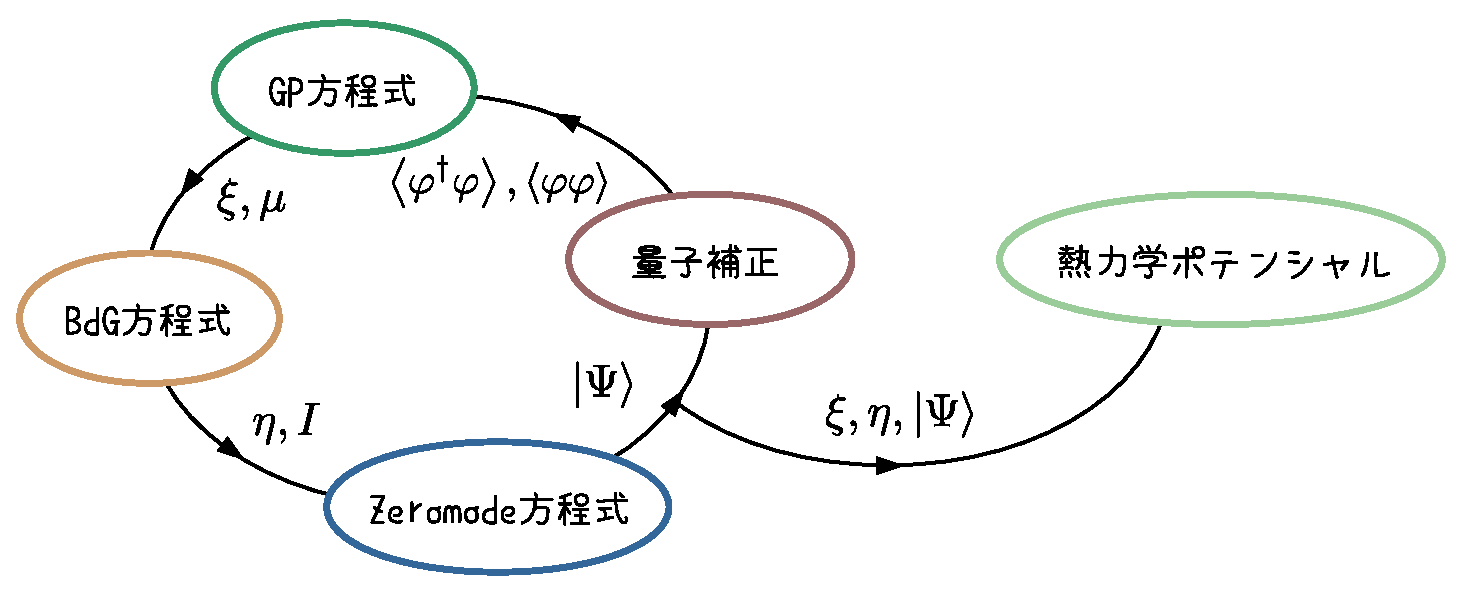
\includegraphics[width = 14cm]{./EPS/self-consistent_new2.eps}
  \end{center}
  \label{self-consistent}
\end{figure}

左の自己無撞着方程式が収束すると$\xi, \eta, \ket{\Psi}$が決まり, それによって分
配関数$Z$や, 熱力学ポテンシャル$\Omega$を(摂動的に)求めることが可能になる.
$\Omega$の摂動展開によって得られた熱力学関数はZeromode-BdG間の相互作用を一部取り
入れたものになっている.
\subsection{量子補正の摂動一次}
有限温度系における量子補正の要は(ざっくり言って)分割条件であり, 本来は相互作用描像で定義された真空$\ket{0}$について
\begin{eqnarray}
  \ev{\varphi_{\rm H}}{0} = 0
\end{eqnarray}
を全ての時刻で満たさなければならない(真空は時間依存しない):
\begin{eqnarray}
  i\partial_t \varphi_{\rm H} &=& \qty[\varphi_{\rm H}, H_{H, 1} + H_{H, 2} + H_{H, 3} + H_{H, 4} ] = 0\\
  i\partial_t \ev{\varphi_{\rm H}}{0} &=& \ev{\qty[\varphi_{\rm H}, H_{H, 1} +  H_{H, 3}] }{0} = 0\\
  \therefore 0 &=& \qty[h_0 - \mu +  g(|\xi|^2 + 2\ev{\varphi_{\rm H}^\dagger\varphi_{\rm H}}{0})]\xi + g\ev{\varphi_{\rm H}\varphi_{\rm H}}{0}\xi^*
\end{eqnarray}
上のとおり, 本来GP方程式に含まれる量子補正はHeisenberg描像の期待値なので議論に一貫性を持たせるためにはこちらも摂動一次を取るべきだと考えられる.

\begin{eqnarray}
  \ev{\varphi_{\rm H}^\dagger(x)\varphi_{\rm H}(x)}{0} &=& \sum_n\qty(\frac{-i}{\hbar})^n\frac{1}{n!}\int_{-\infty}^\infty ds_1 \cdots\int_{-\infty}^\infty ds_n \ev{H_{\rm int}(s_1)\cdots H_{\rm int}(s_n)\varphi^\dagger(x)\varphi(x)}{0}\\
  &\simeq& \ev{\varphi^\dagger(x)\varphi(x)}{0} - i\int_{-\infty}^{\infty}ds\ev{T\qty[H_{\rm int}(s)\varphi^\dagger(x)\varphi(x)]}{0}
\end{eqnarray}
右辺第二項の被積分関数は
\begin{eqnarray}
  \nonumber \ev{T\qty[H_{\rm int}(s)\varphi^\dagger(x)\varphi(x)]}{0} &=& \bra{0}\int d\bm{y}\; T\Bigl[\{\varphi_z^\dagger\calL\varphi_{ex} + \varphi_{ex}^\dagger\calL\varphi_z + \varphi_z\calM^*\varphi_{ex} + \varphi_z^\dagger\calM\varphi_{ex}^\dagger\\
    \nonumber  && +\ g\xi^*(2\varphi_z^\dagger\varphi_z\varphi_{ex} + \varphi_z^\dagger\varphi_{ex}\varphi_{ex} + 2\varphi_{ex}^\dagger\varphi_z\varphi_{ex} + \varphi_{ex}^\dagger\varphi_z\varphi_z)\\
    \nonumber  && +\ g\xi\ (2\varphi_z^\dagger\varphi_{ex}^\dagger\varphi_z + \varphi_z^\dagger\varphi_z^\dagger\varphi_{ex} + 2\varphi_z^\dagger\varphi_{ex}^\dagger\varphi_{ex} + \varphi_{ex}^\dagger\varphi_{ex}^\dagger\varphi_z)\\
    \nonumber  && +\ g(\varphi^\dagger_z\varphi^\dagger_z\varphi_z\varphi_{ex} + \varphi^\dagger_z\varphi^\dagger_{ex}\varphi_z\varphi_z + \varphi_{ex}^\dagger\varphi^\dagger_{ex}\varphi_{ex}\varphi_{z} + \varphi^\dagger_{ex}\varphi^\dagger_{z}\varphi_{ex}\varphi_{ex}) \\
    \nonumber  && +\ \frac{g}{2}\qty(\varphi^\dagger_z \varphi^\dagger_z \varphi_{ex}\varphi_{ex} + 4\varphi^\dagger_z \varphi_z \varphi^\dagger_{ex}\varphi_{ex} + \varphi_z \varphi_z \varphi^\dagger_{ex}\varphi^\dagger_{ex} + \varphi_{ex}^\dagger\varphi_{ex}^\dagger\varphi_{ex}\varphi_{ex})\}\\
    \nonumber&\times& \ul{\varphi_{z}^\dagger(x)\varphi_{z}(x)}_1 + \ul{\varphi^\dagger_{z}(x)\varphi_{ex}(x)}_2 + \ul{\varphi^\dagger_{ex}(x)\varphi_{z}(x)}_3 + \ul{\varphi^\dagger_{ex}(x)\varphi_{ex}(x)}_4\Bigr]\ket{0}\\
\end{eqnarray}
である. $y = (\by, s)$であり, $\by$積分の引数$(y)$は省略している. たとえば, $\ul{\varphi_{z}^\dagger(x)\varphi_{z}(x)}_1$を含む項で生き残る期待値は
\begin{eqnarray}
  \nonumber  &&g\int d\by \bra{0} \Bigl[\varphi^\dagger_z(y) \varphi^\dagger_z(y) \varphi_{ex}(y)\varphi_{ex}(y) + 4\varphi^\dagger_z(y) \varphi_z(y) \varphi^\dagger_{ex}(y)\varphi_{ex}(y)\\
    \nonumber &+& \varphi_z(y) \varphi_z(y) \varphi^\dagger_{ex}(y)\varphi^\dagger_{ex}(y) + \varphi_{ex}^\dagger(y)\varphi_{ex}^\dagger(y)\varphi_{ex}(y)\varphi_{ex}(y)\Bigr]\varphi_{z}^\dagger(x)\varphi_{z}(x)\ket{0}
\end{eqnarray}
となる. これをいちいち演算子のまま処理するのは大変な上, ゼロモードをGreen関数的に取り扱うことは困難. なので, とりあえずゼロモードについては真面目に摂動計算をするのではなく, 摂動ハミルトニアン選択の段階で期待値を取ってc-数的に取り扱う方向に進む. これなら相互作用ハミルトニアン内のゼロモードはBdGモードの係数としてのみ効いてくることになり, 摂動計算は一般的な自発的対称性の破れたBoson場のものとほぼ同一になる. なので, ここから先はゼロモードのない非一様系の摂動計算について考えていくことにする.
\newpage
\section*{Appendix.B  一様系のFormulation}
\renewcommand{\theequation}{B.\arabic{equation}}
\subsection*{B.1  場の展開}
\begin{eqnarray}
  \varphi_{\rm ex} = \frac{1}{\sqrt{(2\pi)^3}}\int d\bm{k} \left[ u_ka_{\bm{k}} + v_k^*a^\dagger_{-\bm{k}} \right]e^{i\bm{k}\bm{x}}
\end{eqnarray}
\subsection*{B.2  各演算子の期待値}
\begin{eqnarray}
  \ev{Q^2(s)}_z &=& \frac{\sum_mq^2\Psi_m(q)e^{-\beta E_m}}{\sum_me^{-\beta E_m}}\\
  \ev{P^2(s)}_z &=& \frac{-\sum_m\frac{d^2}{dq^2}\Psi_m(q)e^{-\beta E_m}}{\sum_me^{-\beta E_m}}\\
  \ev{a_{\bk}^\dagger(s) a_{\bk'}(s)}_{ex} &=& \frac{1}{e^{\beta\omega_{\bk}}-1}\delta(\bk-\bk') \equiv n_{\bk}\delta(\bk - \bk')\\
  \nonumber  \ev{a_{\bk_1}^\dagger(s)a_{\bk_2}^\dagger(s) a_{\bk_3}(s)a_{\bk_4}(s)}_{ex} &=& \qty(\wick{12}{<1a^\dagger_{k1}<2a^\dagger_{k2}>1a_{k3}>2a_{k4}} + \wick{12}{<1a^\dagger_{k1}<2a^\dagger_{k2}>2a_{k3}>1a_{k4}})\\
  &=& n_{\bk_1}n_{\bk_2}\qty{\delta(\bk_1 - \bk_3)\delta(\bk_2 - \bk_4) + \delta(\bk_1 - \bk_4)\delta(\bk_2 - \bk_3)}
\end{eqnarray}
\subsection{B.3  量子補正項}
\begin{eqnarray}
  \ev{\varphi_{ex}\varphi_{ex}}_{ex} &=& \frac{1}{(2\pi)^3}\int d\bk_1\int d\bk_2 \ev{(u_{\bk_1}a_{\bk_1} + v_{\bk_1}^* a^\dagger_{-\bk_1})(u_{\bk_2}a_{\bk_2} + v_{\bk_2}^* a^\dagger_{-\bk_2})}_{ex}e^{i(\bk_1+\bk_2)\cdot \bx}\\
  &=& \frac{1}{(2\pi)^3}\int d\bk_1\int d\bk_2 \ev{(u_{\bk_1}a_{\bk_1} + v_{\bk_1}^* a^\dagger_{-\bk_1})(u_{\bk_2}a_{\bk_2} + v_{\bk_2}^* a^\dagger_{-\bk_2})}_{ex}e^{i(\bk_1+\bk_2)\cdot \bx}\\
  \nonumber &=& \frac{1}{(2\pi)^3}\int d\bk_1\int d\bk_2 \qty(u_{\bk_1}v_{\bk_2}^*\ev{a_{\bk_1} a^\dagger_{-\bk_2}}_{ex}\delta(\bk_1 + \bk_2) + v_{\bk_1}^* u_{\bk_2} \ev{a^\dagger_{-\bk_1}a_{\bk_2}}_{ex}\delta(\bk_1 + \bk_2))e^{i(\bk_1+\bk_2)\cdot \bx}\\
  \\
  &=& \frac{1}{(2\pi)^3}\int d\bk_1\int d\bk_2 \qty(u_{\bk_1}v_{-\bk_1}^*\ev{a_{\bk_1} a^\dagger_{\bk_1}}_{ex}\delta(\bk_1 + \bk_2) + v_{\bk_1}^* u_{-\bk_1} \ev{a^\dagger_{-\bk_1}a_{-\bk_1}}_{ex})\\
  &=& \frac{1}{(2\pi)^3}\int d\bk_1 \qty(u_{\bk_1}v_{-\bk_1}^*\ev{a_{\bk_1} a^\dagger_{\bk_1}}_{ex} + v_{\bk_1}^* u_{-\bk_1} \ev{a^\dagger_{-\bk_1}a_{-\bk_1}}_{ex})\\
  &=& \frac{1}{(2\pi)^3}\int d\bk_1 \qty(1+2n_{\bk})u_{\bk_1}v_{\bk_1} = \frac{1}{(2\pi)^3}\int_{+0}^\infty dk\ k^2\int_0^\pi d\theta\ \sin{\theta}\int_0^{2\pi} d\phi \qty(1+2n_k)u_kv_k\\
  &=& -\frac{1}{(2\pi)^2}\int_{+0}^\infty dk\frac{k^2\calM}{\omega_k}\qty(2n_k + 1)
\end{eqnarray}
となる. $\bk$積分について$\bk = 0$は含まれていないことに注意. この計算では
\begin{itemize}
\item[1. ]$u_{\pm\bk} = u_k, v_{\pm\bk} = v_k, n_{\pm\bk} = n_k$であること
\item[2. ]$\xi, \eta$が実であることで$v_k^* = v_k, u_k^* = u_k$
\item[3. ]$\ev{a_{\bk}a_{\bk}^\dagger}_{ex} = \ev{a_{\bk}^\dagger a_{\bk} + [a_{\bk}, a_{\bk}^\dagger]}_{ex} = 1 + n_k$であること
\item[4. ]$\int_{-\infty}^{\infty} d\bk\ev{a^\dagger_{-\bk}a_{-\bk}}_{ex} = \int_{-\infty}^{\infty} d\bk\ev{a^\dagger_{\bk}a_{\bk}}_{ex} = \int_{-\infty}^{\infty} d\bk n_k$であること
\end{itemize}
などを用いている. 各パラメータは以下の通り:
%$u_k, v_k, n_k, \calL_k...$などは2015夏の学校の資料を参照のこと. 同様にして
\begin{eqnarray}
  \begin{pmatrix}
    u_k\\
    v_k
  \end{pmatrix}
  &=& \frac{1}{\sqrt{2\omega_k}}
  \begin{pmatrix}
    \sqrt{{\cal L}_k + \omega_k}\\
    -\sqrt{{\cal L}_k - \omega_k}
  \end{pmatrix}\\
               {\cal M} = g(\xi^2 - \ev{\varphi\varphi})\hspace{1cm}{\cal L}_k &=& \frac{\hbar^2}{2m}k^2 + {\cal M}\hspace{1cm}\omega_k = \sqrt{\varepsilon_k(\varepsilon_k + 2gn_0)}= \sqrt{{\cal L}^2_k - {\cal M}^2}
\end{eqnarray}
同様にして, 
\begin{eqnarray}
  \ev{\varphi_{ex}^\dagger\varphi_{ex}}_{ex} &=& \frac{1}{(2\pi)^2}\int_0^\infty dk\frac{k^2}{\omega_k}\qty[(2n_k + 1)\calL_k - \omega_k]\\
  \ev{\varphi_{ex}^\dagger\varphi^\dagger_{ex}}_{ex} &=& -\frac{1}{(2\pi)^2}\int_0^\infty dk\frac{k^2\calM}{\omega_k}\qty(2n_k + 1)
\end{eqnarray}
相互作用項は
\begin{eqnarray}
  \nonumber  \ev{\varphi_{ex}^\dagger\varphi_{ex}^\dagger\varphi_{ex}\varphi_{ex}}_{ex} &=& \frac{1}{(2\pi)^6}\int d\bk_1\int d\bk_2\int d\bk_3\int d\bk_4 e^{i(-\bk_1-\bk_2+\bk_3+\bk_4)\cdot \bx}\\
  \nonumber  &\times& \ev{(u_{\bk_1} a_{\bk_1}^\dagger + v_{\bk_1}a_{-\bk_1})(u_{\bk_2} a_{\bk_2}^\dagger + v_{\bk_2}a_{-\bk_2})(u_{\bk_3} a_{\bk_3} + v_{\bk_3}a_{-\bk_3}^\dagger)(u_{\bk_4} a_{\bk_4} + v_{\bk_4}a_{-\bk_4}^\dagger)}_{ex}\\
\end{eqnarray}
である. 生成演算子と消滅演算子が対になっていない期待値は消えてしまうので, 残るものだけを書き下す:
\begin{eqnarray}
  \nonumber  \ev{\varphi_{ex}^\dagger\varphi_{ex}^\dagger\varphi_{ex}\varphi_{ex}}_{ex} &=& \frac{1}{(2\pi)^6}\int d\bk_1\int d\bk_2\int d\bk_3\int d\bk_4 e^{i(-\bk_1-\bk_2+\bk_3+\bk_4)\cdot \bx}\\
  \nonumber  &\times& \Bigl[u_{\bk_1}u_{\bk_2}u_{\bk_3}u_{\bk_4}\ev{a^\dagger_{\bk_1}a^\dagger_{\bk_2}a_{\bk_3}a_{\bk_4}}_{ex} + u_{\bk_1}v_{\bk_2}u_{\bk_3}v_{\bk_4}\ev{a^\dagger_{\bk_1}a_{-\bk_2}a_{\bk_3}a^\dagger_{-\bk_4}}_{ex}\\
    \nonumber    &&+ u_{\bk_1}v_{\bk_2}v_{\bk_3}u_{\bk_4}\ev{a^\dagger_{\bk_1}a_{-\bk_2}a^\dagger_{-\bk_3}a_{\bk_4}}_{ex} + v_{\bk_1}u_{\bk_2}u_{\bk_3}v_{\bk_4}\ev{a_{-\bk_1}a^\dagger_{\bk_2}a_{\bk_3}a^\dagger_{-\bk_4}}_{ex}\\
    \nonumber    &&+ v_{\bk_1}u_{\bk_2}v_{\bk_3}u_{\bk_4}\ev{a_{-\bk_1}a^\dagger_{\bk_2}a^\dagger_{-\bk_3}a_{\bk_4}}_{ex} + v_{\bk_1}v_{\bk_2}v_{\bk_3}v_{\bk_4}\ev{a_{-\bk_1}a_{-\bk_2}a^\dagger_{-\bk_3}a^\dagger_{-\bk_4}}_{ex}\Bigr]\\\label{interaction-expectation}
\end{eqnarray}
Wickの定理で展開:
\begin{eqnarray}
  \nonumber  \ev{a^\dagger_{\bk_1}a^\dagger_{\bk_2}a_{\bk_3}a_{\bk_4}}_{ex} &=& \qty(\wick{12}{<1a^\dagger_{k1}<2a^\dagger_{k2}>1a_{k3}>2a_{k4}} + \wick{21}{<1a^\dagger_{k1}<2a^\dagger_{k2}>2a_{k3}>1a_{k4}})\\
  &=& n_{\bk_1}n_{\bk_2}\qty{\delta(\bk_1 - \bk_3)\delta(\bk_2 - \bk_4) + \delta(\bk_1 - \bk_4)\delta(\bk_2 - \bk_3)}\\
  \nonumber  \ev{a^\dagger_{\bk_1}a_{-\bk_2}a_{\bk_3}a^\dagger_{-\bk_4}}_{ex} &=& \qty(\wick{12}{<1a^\dagger_{k1}>1a_{-k2}<2a_{k3}>2a^\dagger_{-k4}} + \wick{12}{<1a^\dagger_{k1}<2a_{-k2}>1a_{k3}>2a^\dagger_{-k4}})\\
  \nonumber&=& n_{\bk_1}(1 + n_{\bk_3})\delta(\bk_1 + \bk_2)\delta(\bk_3 + \bk_4) + n_{\bk_1}(1 + n_{\bk_2})\delta(\bk_1 - \bk_3)\delta(\bk_2 - \bk_4)\\
  \\
  \nonumber  \ev{a^\dagger_{\bk_1}a_{-\bk_2}a^\dagger_{-\bk_3}a_{\bk_4}}_{ex} &=& \qty(\wick{12}{ <1a^\dagger_{k_1}>1a_{-k_2}<2a^\dagger_{-k_3}>2a_{k_4}} + \wick{21}{<1a^\dagger_{k_1}<2a_{-k_2}>2a^\dagger_{-k_3}>1a_{k_4}})\\
  &=& n_{\bk_1}n_{\bk_3}\delta(\bk_1 + \bk_2)\delta(\bk_3 + \bk_4) + n_{\bk_1}(1 + n_{\bk_2})\delta(\bk_1 - \bk_4)\delta(\bk_2 - \bk_3)\\
  \nonumber  \ev{a_{-\bk_1}a^\dagger_{\bk_2}a_{\bk_3}a^\dagger_{-\bk_4}}_{ex} &=& \qty(\wick{12}{<1a_{-k_1}>1a^\dagger_{k_2}<2a_{k_3}>2a^\dagger_{-k_4}} + \wick{21}{<1a_{-k_1}<2a^\dagger_{k_2}>2a_{k_3}>1a^\dagger_{-k_4}})\\
  \nonumber&=& (1+n_{\bk_1})(1+n_{\bk_3})\delta(\bk_1 + \bk_2)\delta(\bk_3 + \bk_4) + (1+n_{\bk_1})n_{\bk_2}\delta(\bk_1 - \bk_4)\delta(\bk_2 - \bk_3)\\
  \\
  \nonumber  \ev{a_{-\bk_1}a^\dagger_{\bk_2}a^\dagger_{-\bk_3}a_{\bk_4}}_{ex} &=& \qty(\wick{12}{<1a_{-k_1}>1a^\dagger_{k_2}<2a^\dagger_{-k_3}>2a_{k_4}} + \wick{12}{<1a_{-k_1}<2a^\dagger_{k_2}>1a^\dagger_{-k_3}>2a_{k_4}})\\
  &=& (1 + n_{\bk_1})n_{\bk_3}\delta(\bk_1 + \bk_2)\delta(\bk_3 + \bk_4) + (1 + n_{\bk_1})n_{\bk_2}\delta(\bk_1 - \bk_3)\delta(\bk_2 - \bk_4)\\
  \nonumber  \ev{a_{-\bk_1}a_{-\bk_2}a^\dagger_{-\bk_3}a^\dagger_{-\bk_4}}_{ex} &=& \qty(\wick{12}{<1a_{-k_1}<2a_{-k_2}>1a^\dagger_{-k_3}>2a^\dagger_{-k_4}} + \wick{21}{<1a_{-k_1}<2a_{-k_2}>2a^\dagger_{-k_3}>1a^\dagger_{-k_4}})\\
  &=& (1 + n_{\bk_1})(1 + n_{\bk_2})\qty{\delta(\bk_1 - \bk_3)\delta(\bk_2 - \bk_4) + \delta(\bk_1 - \bk_4)\delta(\bk_2 - \bk_3)}
\end{eqnarray}
これらを(\ref{interaction-expectation})に代入すると
\begin{eqnarray}
  \ev{\varphi_{ex}^\dagger\varphi_{ex}^\dagger\varphi_{ex}\varphi_{ex}}_{ex} &=& \frac{1}{(2\pi)^6}\qty[2\qty(I_u'^{, 2} + I_v'^{+, 2} +  I_u'I_v'^{+} + I_{uv}I_{uv}^+) + I_{uv}^2 + I_u'I_v'^+ + I_{uv}^{+, 2} + I_u'^{+}I_v']\\
  &=& \frac{1}{(2\pi)^6}\qty[2\qty(I_u'^{, 2} + I_v'^{+, 2} +  I_u'I_v'^{+}) + \qty(I_{uv} + I_{uv}^{+})^2+ I_u'I_v'^+  + I_u'^{+}I_v']\\
  &=& \frac{1}{(2\pi)^6}\qty[2\qty(I_u'^{, 2} + I_v'^{+, 2}) + \qty(I_{uv} + I_{uv}^{+})^2+ 4I_u'I_v'^+]
\end{eqnarray}
となる. ただし
\begin{eqnarray}
  \nonumber I_u' &=& \int d\bk n_{\bk} u_{\bk}^2\hspace{1cm}I_v' = \int d\bk n_{\bk} v_{\bk}^2\hspace{1cm} I_{uv} = \int d\bk n_{\bk} u_{\bk}v_{\bk}\\
  \nonumber I_{uv}^+ &=& \int d\bk (1 + n_{\bk}) u_{\bk}v_{\bk} \hspace{1cm}I_v'^+ = \int d\bk (1 + n_{\bk}) v_{\bk}^2\hspace{1cm}I_u'^+ = \int d\bk (1 + n_{\bk}) u_{\bk}^2\\
\end{eqnarray}
であり, かつ$I_u'I_v'^+ = I_u'^+I_v'$であることを用いている.

以上で具体的にゼロモード・励起モードの期待値が計算できたので,
(\ref{Hamiltonian-Exp})に(\ref{Zeromode-Exp}), (\ref{BdG-Exp}),
(\ref{Interaction-Exp})を代入する.$I$はすべて$\bx$依存性を持たないので空間積分は系の体積$V$が出てくるだけ.
まとめると, (\ref{Hamiltonian-Exp})は
\begin{eqnarray}
  \nonumber  \ev{H_{\rm int}}_0 =&& \int d\bx\Bigl[-\frac{2}{(2\pi)^2}\qty(-\xi^2\ev{Q^2}_z + \eta^2\ev{P^2}_z)\int_{+0}^\infty dk\frac{k^2\calM}{\omega_k}\qty(2n_k + 1)\\
    &+& \frac{4}{(2\pi)^2}\qty(\xi^2\ev{Q^2}_z + \eta^2\ev{P^2}_z)\int_0^\infty dk\frac{k^2}{\omega_k}\qty{(2n_k + 1)\calL_k - \omega_k}\\
    &+& \frac{1}{(2\pi)^6}\qty{2\qty(I_u'^{, 2} + I_v'^{+, 2}) + \qty(I_{uv} + I_{uv}^{+})^2+ 4I_u'I_v'^+}\Bigr]
\end{eqnarray}
\renewcommand{\theequation}{\thechapter.\arabic{equation}}

\newpage
\chapter{研究 : ゼロモードがない非一様接触型Boson系について}
\begin{itemize}
\item $t$の並進対称性からFourier変換可能($\bk$のFourier変換は不可). Sokhotski-Plemeljの公式をちゃんと処理できる.
\item まずはBdGモードについての1次の摂動をちゃんと計算する!
\item それができたら, proper-diagramの計算ができるのでは? ただし有限サイズ系なので離散になっている. 一様系のラダー近似は離散系にどれだけ適応可能か?
\item ゼロモードについては平均場みたいにしてハミルトニアンに繰り込む形にする. そうすればFeynman diagramが使える. ゼロモードの(厳密な)Wickは諦める. 
\end{itemize}
まずはゼロモードがない場合の摂動一次をしっかりと計算することを目指す. 
\section{1次のGreen関数の計算}
摂動ハミルトニアンを
\begin{eqnarray}
  H_{\rm int} = g\int d\bx \qty(\xi \varphi_{\rm ex}^\dagger(x)\varphi_{\rm ex}^\dagger(x)\varphi_{\rm ex}(x) + \xi^*(x)\varphi_{\rm ex}^\dagger(x)\varphi_{\rm ex}(x)\varphi_{\rm ex}(x) + \frac12\varphi_{\rm ex}^\dagger(x)\varphi_{\rm ex}^\dagger(x)\varphi_{\rm ex}(x)\varphi_{\rm ex}(x))
\end{eqnarray}
のようにとったとき, 量子補正の摂動一次は
\begin{eqnarray}
  &&-i\int_{-\infty}^{\infty} ds\ev{T\qty[H_{\rm int}(s)\varphi^\dagger_{\rm ex}(x)\varphi_{\rm ex}(x)]}\\
  &=& \frac{-ig}{2}\int_{-\infty}^{\infty}\; ds\int\; d\by \ev{T\qty[\varphi_{\rm ex}^\dagger(y)\varphi_{\rm ex}^\dagger(y)\varphi_{\rm ex}(y)\varphi_{\rm ex}(y)\varphi^\dagger(x)\varphi(x)]}
\end{eqnarray}
である. ハミルトニアンの奇数次項は摂動一次でも奇数次になるので落ちる. 以降は$\varphi_{ex}\rightarrow \varphi$と書くことにする. これをWickの定理で分解する\footnote{$\ev{\varphi^\dagger(x)\varphi(x)}$の組み合わせもありそうだが, disconnectedなダイアグラムになるので除外している. }:
\begin{eqnarray}
  &&\frac{-ig}{2}\int_{-\infty}^{\infty}\; ds\int\; d\by \ev{T\qty[\varphi^\dagger(y)\varphi^\dagger(y)\varphi(y)\varphi(y)\varphi^\dagger(x)\varphi(x)]}\\
  \nonumber  &=& \frac{-ig}{2}\int_{-\infty}^{\infty}\; ds\int\; d\by\; \Bigl[2\ev{T\qty[\varphi^\dagger(y)\varphi^\dagger(x)]}\ev{T\qty[\varphi^\dagger(y)\varphi(x)]}\ev{\varphi(y)\varphi(y)}\\
    \nonumber    &&\hspace{3cm}+4\ev{T\qty[\varphi^\dagger(y)\varphi^\dagger(x)]}\ev{T\qty[\varphi(y)\varphi(x)]}\ev{\varphi^\dagger(y)\varphi(y)}\\
    \nonumber&&\hspace{3cm}+2\ev{T\qty[\varphi(y)\varphi^\dagger(x)]}\ev{T\qty[\varphi(y)\varphi(x)]}\ev{\varphi^\dagger(y)\varphi^\dagger(y)}\\
    &&\hspace{3cm}+ 4\ev{T\qty[\varphi(y)\varphi^\dagger(x)]}\ev{T\qty[\varphi^\dagger(y)\varphi(x)]}\ev{\varphi^\dagger(y)\varphi(y)}\Bigr]\label{Green_1st}
\end{eqnarray}
ここには同時刻Green関数が含まれるが, 相互作用ハミルトニアンの4次には常に$\varphi^\dagger$が$\varphi$の左側にあることを根拠に定義される. 
\subsection{Green関数の1行目の具体計算}
いくつかのGreen関数に分解できたので, そのうちの一つを具体的に計算する. まず上式の第一項を計算することを目標にする
\begin{eqnarray}
  \ev{T\qty[\varphi^\dagger(y)\varphi(x)]} &=&\ev{\theta(t-s)\varphi(x)\varphi^\dagger(y)+\theta(s-t)\varphi^\dagger(y)\varphi(x)}\\
  \nonumber  &=&\ev{\theta(t-s)\sum_{j_1, j_2}\qty(u_{j_1}(\bx)a_{j_1}(t) + v_{j_1}^*(\bx)a_{j_1}^\dagger(t))\qty(u_{j_2}^*(\by)a_{j_2}^\dagger(s) + v_{j_2}(\by)a_{j_2}(s))}\\
  \nonumber  &&+ \ev{\theta(s-t)\sum_{j_1, j_2}\qty(u_{j_1}^*(\by)a_{j_1}^\dagger(s) + v_{j_1}(\by)a_{j_1}(s))\qty(u_{j_2}(\bx)a_{j_2}(t) + v^*_{j_2}(\bx)a^\dagger_{j_2}(t))}\\
  \nonumber&=&\theta(t-s)\sum_{j_1}\qty(u_{j_1}(\bx)u_{j_1}^*(\by)\ev{a_{j_1}(t)a_{j_1}^\dagger(s)} + v_{j_1}^*(\bx)v_{j_1}(\by)\ev{a_{j_1}^\dagger(t)a_{j_1}(s)})\\
  &&+\theta(s-t)\sum_{j_1}\qty(u_{j_1}^*(\by)u_{j_1}(\bx)\ev{a_{j_1}^\dagger(s)a_{j_1}(t)} + v_{j_1}(\by)v_{j_1}^*(\bx)\ev{a_{j_1}(s)a_{j_1}^\dagger(t)})
\end{eqnarray}
ここでは, いずれ$\ev{a_{j_1}^\dagger a_{j_2}}, \ev{a_{j_1} a_{j_2}^\dagger}$からクロネッカーデルタ$\delta_{j_1, j_2}$が出てくることを見越して和をひとつ減らしている. 同様にして
\begin{eqnarray}
  \ev{T\qty[\varphi^\dagger(y)\varphi^\dagger(x)]} &=&\ev{\theta(t-s)\varphi^\dagger(x)\varphi^\dagger(y)+\theta(s-t)\varphi^\dagger(y)\varphi^\dagger(x)}\\
  \nonumber  &=&\ev{\theta(t-s)\sum_{j_1, j_2}\qty(u^*_{j_1}(\bx)a^\dagger_{j_1}(t) + v_{j_1}(\bx)a_{j_1}(t))\qty(u_{j_2}^*(\by)a_{j_2}^\dagger(s) + v_{j_2}(\by)a_{j_2}(s))}\\
  \nonumber  &&+ \ev{\theta(s-t)\sum_{j_1, j_2}\qty(u_{j_1}^*(\by)a_{j_1}^\dagger(s) + v_{j_1}(\by)a_{j_1}(s))\qty(u^*_{j_2}(\bx)a^\dagger_{j_2}(t) + v_{j_2}(\bx)a_{j_2}(t))}\\
  \nonumber&=& \theta(t-s)\sum_{j_1}\qty(u^*_{j_1}(\bx)v_{j_1}(\by)\ev{a_{j_1}^\dagger(t)a_{j_1}(s)} + v_{j_1}(\bx)u^*_{j_1}(\by)\ev{a_{j_1}(t)a_{j_1}^\dagger(s)})\\
  &&+\theta(s-t)\sum_{j_1}\qty(u^*_{j_1}(\by)v_{j_1}(\bx)\ev{a_{j_1}^\dagger(s)a_{j_1}(t)} + v_{j_1}(\by)u^*_{j_1}(\bx)\ev{a_{j_1}(s)a_{j_1}^\dagger(t)})
\end{eqnarray}
次はT積がない項:
\begin{eqnarray}
  \ev{\varphi(y)\varphi(y)} &=& \ev{\sum_{j_1, j_2}\qty(u_{j_1}(\by)a_{j_1}(s) + v_{j_1}^*(\by)a_{j_1}^\dagger(s))\qty(u_{j_2}(\by)a_{j_2}(s) + v^*_{j_2}(\by)a^\dagger_{j_2}(s))}\\
  &=& \sum_{j_1}\qty(u_{j_1}(\by)v^*_{j_1}(\by)\ev{a_{j_1}(s)a^\dagger_{j_1}(s)} + v_{j_1}^*(\by)u_{j_1}(\by)\ev{a_{j_1}^\dagger(s)a_{j_1}(s)})
\end{eqnarray}
ここまでできたら上3つの積をまとめる $\theta$関数のクロスタームは消えることを利用すると以下のようになる:
\begin{eqnarray}
  &&\qty{\ev{T\qty[\varphi^\dagger(y)\varphi^\dagger(x)]}\ev{T\qty[\varphi^\dagger(y)\varphi(x)]}\ev{\varphi(y)\varphi(y)}}^{\mu\nu\lambda}_{\mu'\nu'\lambda'}\\
  \nonumber  &=& \sum_{j_1, j_2, j_3}\theta(t-s)\times\\
  \nonumber  &&\begin{Bmatrix}
    u_{1}(\bx)u_{1}^*(\by)\ev{a_{1}a_{1}^\dagger}e^{-i\omega_1(t-s)}\\
    v_{1}^*(\bx)v_{1}(\by)\ev{a_{1}^\dagger a_{1}}e^{i\omega_1(t-s)}
  \end{Bmatrix}^\mu
  \begin{Bmatrix}
    v_{2}(\bx)u^*_{2}(\by)\ev{a_{2}a_{2}^\dagger}e^{-i\omega_2(t-s)}\\
    u^*_{2}(\bx)v_{2}(\by)\ev{a_{2}^\dagger a_{2}}e^{i\omega_2(t-s)}
  \end{Bmatrix}^\nu
  \begin{Bmatrix}
    u_{3}(\by)v^*_{3}(\by)\ev{a_{3}a^\dagger_{3}}\\
    v_{3}^*(\by)u_{3}(\by)\ev{a_{3}^\dagger a_{3}}
  \end{Bmatrix}^\lambda\\
  \nonumber  &&+ \sum_{j_1, j_2, j_3}\theta(s-t)\times\\
  \nonumber  &&\begin{Bmatrix}
    u_{1}^*(\by)u_{1}(\bx)\ev{a_{1}^\dagger a_{1}}e^{-i\omega_1(t-s)}\\
    v_{1}(\by)v_{1}^*(\bx)\ev{a_{1}a_{1}^\dagger}e^{i\omega_1(t-s)}
  \end{Bmatrix}^{\mu'}
  \begin{Bmatrix}
    u^*_{2}(\by)v_{2}(\bx)\ev{a_{2}^\dagger a_{2}}e^{-i\omega_2(t-s)}\\
    v_{2}(\by)u^*_{2}(\bx)\ev{a_{2}a_{2}^\dagger}e^{i\omega_2(t-s)}
  \end{Bmatrix}^{\nu'}
  \begin{Bmatrix}
    u_{3}(\by)v^*_{3}(\by)\ev{a_{3}a^\dagger_{3}}\\
    v_{3}^*(\by)u_{3}(\by)\ev{a_{3}^\dagger a_{3}}
  \end{Bmatrix}^{\lambda'}\\
\end{eqnarray}
ここで$j_i\rightarrow i$と省略し, かつ項が多すぎるのでテンソル形式を用いている. $\mu, \nu, \lambda$はそれぞれ$(-, +)$の2種類. テンソルの添字は上が$-$に対応しており, 時間成分は$-i\omega\tau$, 下は$+$に対応しており, 時間成分は$i\omega\tau$である.   これを時間$t-s = \tau$についてFourier変換する:
\begin{eqnarray}
  &&\frac{1}{\sqrt{2\pi}}\int\; d\tau\;e^{i\omega\tau}  \qty{\ev{T\qty[\varphi^\dagger(y)\varphi^\dagger(x)]}\ev{T\qty[\varphi^\dagger(y)\varphi(x)]}\ev{\varphi(y)\varphi(y)}}^{\mu\nu\lambda}_{\mu'\nu'\lambda'}\\
  \nonumber  &=& \frac{1}{\sqrt{2\pi}}\int\; d\tau\;e^{i\omega\tau}\sum_{j_1, j_2, j_3}\theta(\tau)\times\\
  \nonumber  &&\begin{Bmatrix}
    u_{1}(\bx)u_{1}^*(\by)\ev{a_{1}a_{1}^\dagger}e^{-i\omega_1\tau}\\
    v_{1}^*(\bx)v_{1}(\by)\ev{a_{1}^\dagger a_{1}}e^{i\omega_1\tau}
  \end{Bmatrix}^\mu
  \begin{Bmatrix}
    v_{2}(\bx)u^*_{2}(\by)\ev{a_{2}a_{2}^\dagger}e^{-i\omega_2\tau}\\
    u^*_{2}(\bx)v_{2}(\by)\ev{a_{2}^\dagger a_{2}}e^{i\omega_2\tau}
  \end{Bmatrix}^\nu
  \begin{Bmatrix}
    u_{3}(\by)v^*_{3}(\by)\ev{a_{3}a^\dagger_{3}}\\
    v_{3}^*(\by)u_{3}(\by)\ev{a_{3}^\dagger a_{3}}
  \end{Bmatrix}^\lambda\\
  \nonumber  &&+ \frac{1}{\sqrt{2\pi}}\int\; d\tau\;e^{i\omega\tau}\sum_{j_1, j_2, j_3}\theta(-\tau)\times\\
  \nonumber  &&\begin{Bmatrix}
    u_{1}^*(\by)u_{1}(\bx)\ev{a_{1}^\dagger a_{1}}e^{-i\omega_1\tau}\\
    v_{1}(\by)v_{1}^*(\bx)\ev{a_{1}a_{1}^\dagger}e^{i\omega_1\tau}
  \end{Bmatrix}^{\mu'}
  \begin{Bmatrix}
    u^*_{2}(\by)v_{2}(\bx)\ev{a_{2}^\dagger a_{2}}e^{-i\omega_2\tau}\\
    v_{2}(\by)u^*_{2}(\bx)\ev{a_{2}a_{2}^\dagger}e^{i\omega_2\tau}
  \end{Bmatrix}^{\nu'}
  \begin{Bmatrix}
    u_{3}(\bx)v^*_{3}(\by)\ev{a_{3}a^\dagger_{3}}\\
    v_{3}^*(\bx)u_{3}(\by)\ev{a_{3}^\dagger a_{3}}
  \end{Bmatrix}^{\lambda'}\\
\end{eqnarray}
Sokhotski-Plemeljの公式\footnote{$\theta$関数の積分表示を使ってすぐに証明可能.}
\begin{eqnarray}
  \int_{-\infty}^\infty ds\; \theta(t-s)e^{-i\varepsilon(s-t)} &=& \int_{-\infty}^t ds e^{-i\varepsilon(s-t)} = {\cal P}\frac{i}{\varepsilon} + \pi\delta(\varepsilon)\\
  \int_{-\infty}^\infty ds\; \theta(s-t)e^{-i\varepsilon(s-t)} &=& \int_{t}^{\infty} ds e^{-i\varepsilon(s-t)} = -{\cal P}\frac{i}{\varepsilon} + \pi\delta(\varepsilon)
\end{eqnarray}
を用いて$\tau$-積分を処理:
\begin{eqnarray}
  &&\frac{1}{\sqrt{2\pi}}\int\; d\tau\;e^{i\omega\tau}  \qty{\ev{T\qty[\varphi^\dagger(y)\varphi^\dagger(x)]}\ev{T\qty[\varphi^\dagger(y)\varphi(x)]}\ev{\varphi(y)\varphi(y)}}^{\mu\nu\lambda}_{\mu'\nu'\lambda'}\\
  \nonumber  &=& \frac{1}{\sqrt{2\pi}}\sum_{j_1, j_2, j_3}\\
  \nonumber  && \begin{Bmatrix}
    u_{1}(\bx)u_{1}^*(\by)\ev{a_{1}a_{1}^\dagger}\\
    v_{1}^*(\bx)v_{1}(\by)\ev{a_{1}^\dagger a_{1}}
  \end{Bmatrix}^\mu
  \begin{Bmatrix}
    v_{2}(\bx)u^*_{2}(\by)\ev{a_{2}a_{2}^\dagger}\\
    u^*_{2}(\bx)v_{2}(\by)\ev{a_{2}^\dagger a_{2}}
  \end{Bmatrix}^\nu
  \begin{Bmatrix}
    u_{3}(\by)v^*_{3}(\by)\ev{a_{3}a^\dagger_{3}}\\
    v_{3}^*(\by)u_{3}(\by)\ev{a_{3}^\dagger a_{3}}
  \end{Bmatrix}^\lambda \qty(-{\cal P}\frac{i}{\omega - \omega^{\mu\nu}} + \pi\delta(\omega - \omega^{\mu\nu}))\\
  \nonumber  &&+\begin{Bmatrix}
  u_{1}^*(\by)u_{1}(\bx)\ev{a_{1}^\dagger a_{1}}\\
  v_{1}(\by)v_{1}^*(\bx)\ev{a_{1}a_{1}^\dagger}
  \end{Bmatrix}^{\mu'}
  \begin{Bmatrix}
    u^*_{2}(\by)v_{2}(\bx)\ev{a_{2}^\dagger a_{2}}\\
    v_{2}(\by)u^*_{2}(\bx)\ev{a_{2}a_{2}^\dagger}
  \end{Bmatrix}^{\nu'}
  \begin{Bmatrix}
    u_{3}(\by)v^*_{3}(\by)\ev{a_{3}a^\dagger_{3}}\\
    v_{3}^*(\by)u_{3}(\by)\ev{a_{3}^\dagger a_{3}}
  \end{Bmatrix}^{\lambda'}\qty({\cal P}\frac{i}{\omega - \omega^{\mu'\nu'}} + \pi\delta(\omega - \omega^{\mu'\nu'}))\\
\end{eqnarray}
ここで$\mu, \nu, \lambda$の符号はそのまま$\omega_i$の符号に対応しており, 例えば
\begin{eqnarray}
  &&\omega^{-+} = -\omega_1 + \omega_2
\end{eqnarray}
である. 時間のFourier変換である$\omega$を主値積分とデルタ関数という形でくくり出せたので, これを逆Fourier変換しつつ, $s$-積分を実行する:
\begin{eqnarray}
  &&\frac{1}{\sqrt{2\pi}} \int\;ds\int\;d\omega\; e^{-i\omega\tau}\qty(-{\cal P}\frac{i}{\omega - \omega^{\mu\nu}} + \pi\delta(\omega - \omega^{\mu\nu}))\\
  &=&\frac{1}{\sqrt{2\pi}}\int\;ds\qty(-i{\cal P}\int\;\frac{d\omega e^{-i\omega\tau}}{\omega - \omega^{\mu\nu}} + \frac{\pi}{2}e^{-i\omega^{\mu\nu}\tau})\\
  &=& \frac{1}{\sqrt{2\pi}}\qty(-2\pi i{\cal P}\int\;\frac{d\omega \delta(\omega)e^{-i\omega t}}{\omega - \omega^{\mu\nu}} + \frac{\pi}{2}\delta(\omega^{\mu\nu})e^{-i\omega^{\mu\nu}t})\\
  &\simeq&\sqrt{2\pi}\frac{i}{\omega^{\mu\nu}}
\end{eqnarray}
最後の行では$\omega^{\mu\nu\lambda}$がぴったりゼロになることはあまり無いだろうという仮定をしている\footnote{残すべきかもしれないが, 少なくともこのデルタ関数を処理するような積分は現れないし, 引数の$\omega^{\mu\nu\lambda}$は離散的. 仮にトラップポテンシャル$V(\bx)$が無ければ励起は等間隔になる. 例えば$\omega_{j_1 = 1} - \omega_{j_2 = 0} - \omega_{j_3 = 0} = 2\hbar\omega -\hbar\omega - \hbar\omega = 0$のようにきれいにゼロになってしまい, 他にも無数の組み合わせが存在する. 今回は相互作用込みのBdGなので厳密に等間隔にはならない.}. これで(\ref{Green_1st})の一行目は
\begin{eqnarray}
  \nonumber &&\frac{-ig}{2}\int_{-\infty}^{\infty}\; ds\int\; d\by \ev{T\qty[\varphi^\dagger(y)\varphi^\dagger(y)\varphi(y)\varphi(y)\varphi^\dagger(x)\varphi(x)]}_{1行目}\\
  \nonumber  &=& \frac{-ig}{2}\int_{-\infty}^{\infty}\; ds\int\; d\by\; \qty[2\ev{T\qty[\varphi^\dagger(y)\varphi^\dagger(x)]}\ev{T\qty[\varphi^\dagger(y)\varphi(x)]}\ev{\varphi(y)\varphi(y)}]\\
  \nonumber  &\simeq& g\int d\by \sum_{j_1, j_2, j_3}\frac{1}{\omega^{\mu\nu}}
  \begin{Bmatrix}
    u_{1}(\bx)u_{1}^*(\by)\ev{a_{1}a_{1}^\dagger}\\
    v_{1}^*(\bx)v_{1}(\by)\ev{a_{1}^\dagger a_{1}}
  \end{Bmatrix}^\mu
  \begin{Bmatrix}
    v_{2}(\bx)u^*_{2}(\by)\ev{a_{2}a_{2}^\dagger}\\
    u^*_{2}(\bx)v_{2}(\by)\ev{a_{2}^\dagger a_{2}}
  \end{Bmatrix}^\nu
  \begin{Bmatrix}
    u_{3}(\by)v^*_{3}(\by)\ev{a_{3}a^\dagger_{3}}\\
    v_{3}^*(\by)u_{3}(\by)\ev{a_{3}^\dagger a_{3}}
  \end{Bmatrix}^\lambda\\
  &&- \frac{1}{\omega^{\mu'\nu'}}
  \begin{Bmatrix}
    u_{1}^*(\by)u_{1}(\bx)\ev{a_{1}^\dagger a_{1}}\\
    v_{1}(\by)v_{1}^*(\bx)\ev{a_{1}a_{1}^\dagger}
  \end{Bmatrix}^{\mu'}
  \begin{Bmatrix}
    u^*_{2}(\by)v_{2}(\bx)\ev{a_{2}^\dagger a_{2}}\\
    v_{2}(\by)u^*_{2}(\bx)\ev{a_{2}a_{2}^\dagger}
  \end{Bmatrix}^{\nu'}
  \begin{Bmatrix}
    u_{3}(\by)v^*_{3}(\by)\ev{a_{3}a^\dagger_{3}}\\
    v_{3}^*(\by)u_{3}(\by)\ev{a_{3}^\dagger a_{3}}
  \end{Bmatrix}^{\lambda'}
\end{eqnarray}
面倒ではあるが, 書き下すことができた. 時間成分は無くなったが, 添字$\mu, \nu, \lambda$についてはテンソルの上部が$-$, 下部が$+$に対応している\footnote{もちろん, 区別さえつけば添字はなんだっていい. }. もちろん$\ev{a^\dagger a}, \ev{a a^\dagger}$はBose-Einstein分布関数で表せる.

テンソル積の引き算になっているのでうまく消える項があるかもしれないし, 実際に計算するときは$\xi$が実であることを仮定して$u, v$も実になるので, もっと綺麗になるかもしれない\footnote{流石にゼロになることは無いと信じたいが...まだ計算してないのでそれもわからない.}.

後にAll-orderの計算をすることになるが, その定式化が完了してかつ実効的に計算が可能であれば今回のように摂動一次に限って計算する必要はなくなるが, 今回のGreen関数の時間成分の処理に関するテクニックは今後(恐らく)重要になってくるので, その時のための練習だと思うと良い. 
\subsection{Green関数の2行目以降}
手順は同じなので省略. 
\section{All-orderの計算に向けて:その1}
非一様系でLadder diagramの無限次を取り込んで計算することを目指す. まず一様系ではどのようにして無限次まで取り入れることを可能にしているのか, 非一様系ではどのような困難があるのかを確認することがまず目標とするところ.
\subsection{1次のself-energyの具体形}
自発的対称性が破れているBoson系を扱っているので, $\ev{T\qty[\varphi\varphi]}, \ev{T\qty[\varphi^\d\varphi^\d]}$のようなanomalous-Green関数(異常Green関数)が値を持つことになる. それに応じてGreen関数は$2\times2$のテンソルに拡張される.

Dyson方程式:
\begin{eqnarray}
  G^{\mu\nu}(x_1, x_2) = G_0^{\mu\nu}(x_1, x_2) + \int d^4y_1d^4y_2\;G_0^{\mu\mu'}(x_1, y_1)\Sigma^{\mu'\nu'}(y_1, y_2)G^{\nu'\nu}(y_2, x_2)
\end{eqnarray}
について, 1次の項を拾ってくる:
\begin{eqnarray}
  G^{\mu\nu}_1(x_1, x_2) =  \int d^4y_1d^4y_2\;G_0^{\mu\mu'}(x_1, y_1)\Sigma_1^{\mu'\nu'}(y_1, y_2)G_0^{\nu'\nu}(y_2, x_2)
\end{eqnarray}
Green関数及びself-energyは
\begin{eqnarray}
  G^{\mu\nu}(x_1, x_2) &=&
  \begin{bmatrix}
    G^{11}(x_1, x_2)&G^{12}(x_1, x_2)\\
    G^{21}(x_1, x_2)&G^{22}(x_1, x_2)
  \end{bmatrix}^{\mu\nu} =
  \begin{bmatrix}
    \ev{T\qty[\varphi_{\rm H}(x_1)\varphi_{\rm H}^\dagger(x_2)]}&\ev{T\qty[\varphi_{\rm H}(x_1)\varphi_{\rm H}(x_2)]}\\
    \ev{T\qty[\varphi_{\rm H}^\dagger(x_1)\varphi_{\rm H}^\dagger(x_2)]}&\ev{T\qty[\varphi_{\rm H}^\dagger(x_1)\varphi_{\rm H}(x_2)]}
  \end{bmatrix}^{\mu\nu}\\
  \Sigma^{\mu\nu}(x_1, x_2) &=&
  \begin{bmatrix}
    \Sigma^{11}(x_1, x_2)&\Sigma^{12}(x_1, x_2)\\
    \Sigma^{21}(x_1, x_2)&\Sigma^{22}(x_1, x_2)
  \end{bmatrix}^{\mu\nu}
\end{eqnarray}
これに対して具体的なGreen関数の摂動一次は
\begin{eqnarray}
  \nonumber  G^{22}_1(x, x) &=& \int d^4y_1d^4y_2\;G_0^{2\mu'}(x, y_1)\Sigma_1^{\mu'\nu'}(y_1, y_2)G_0^{\nu'2}(y_2, x)\\
  \nonumber  &=& \frac{-ig}{2}\int d^4y_1\; \Bigl[2\ev{T\qty[\varphi^\dagger(x)\varphi^\dagger(y_1)]}\ev{\varphi(y_1)\varphi(y_1)}\ev{T\qty[\varphi^\dagger(y_1)\varphi(x)]}\\
    \nonumber    &&\hspace{2cm}+4\ev{T\qty[\varphi^\dagger(x)\varphi^\dagger(y_1)]}\ev{\varphi^\dagger(y_1)\varphi(y_1)}\ev{T\qty[\varphi(y_1)\varphi(x)]}\\
    &&\hspace{2cm}+2\ev{T\qty[\varphi^\dagger(x)\varphi(y_1)]}\ev{\varphi^\dagger(y_1)\varphi^\dagger(y_1)}\ev{T\qty[\varphi(y_1)\varphi(x)]}\\
    &&\hspace{2cm}+ 4\ev{T\qty[\varphi^\dagger(x)\varphi(y_1)]}\ev{\varphi^\dagger(y_1)\varphi(y_1)}\ev{T\qty[\varphi^\dagger(y_1)\varphi(x)]}
    \Bigr]
\end{eqnarray}
なので, 1次のDyson方程式と比較することでself-energyを求めることができる:
\begin{eqnarray}
  \Sigma^{\mu'\nu'}_1(y_1, y_2) &=& -ig\delta(y_1-y_2)
  \begin{bmatrix}
    2\ev{\varphi^\dagger(y_1)\varphi(y_1)}&\ev{\varphi^\dagger(y_1)\varphi^\dagger(y_1)}\\
    \ev{\varphi(y_1)\varphi(y_1)}&2\ev{\varphi^\dagger(y_1)\varphi(y_1)}
  \end{bmatrix}^{\mu'\nu'}\label{1st-self-energy}
\end{eqnarray}
\subsection{梯子近似されたBethe-Salpeter方程式へ}
前節で1次のself-energyを求めたが, これはGreen関数の1次の展開をself-energyで言い換えただけである. 以下, self-energyについてもう少し詳しく考えてみる.
repulsive core(1点で無限大になるようなポテンシャル)を持つような系では図 \ref{ladder1}のような梯子型のダイアグラムが強く寄与する\footnote{らしい. ちゃんとした理由はまだよく理解できてない. }.
\begin{figure}[htbp]
  \begin{center}
    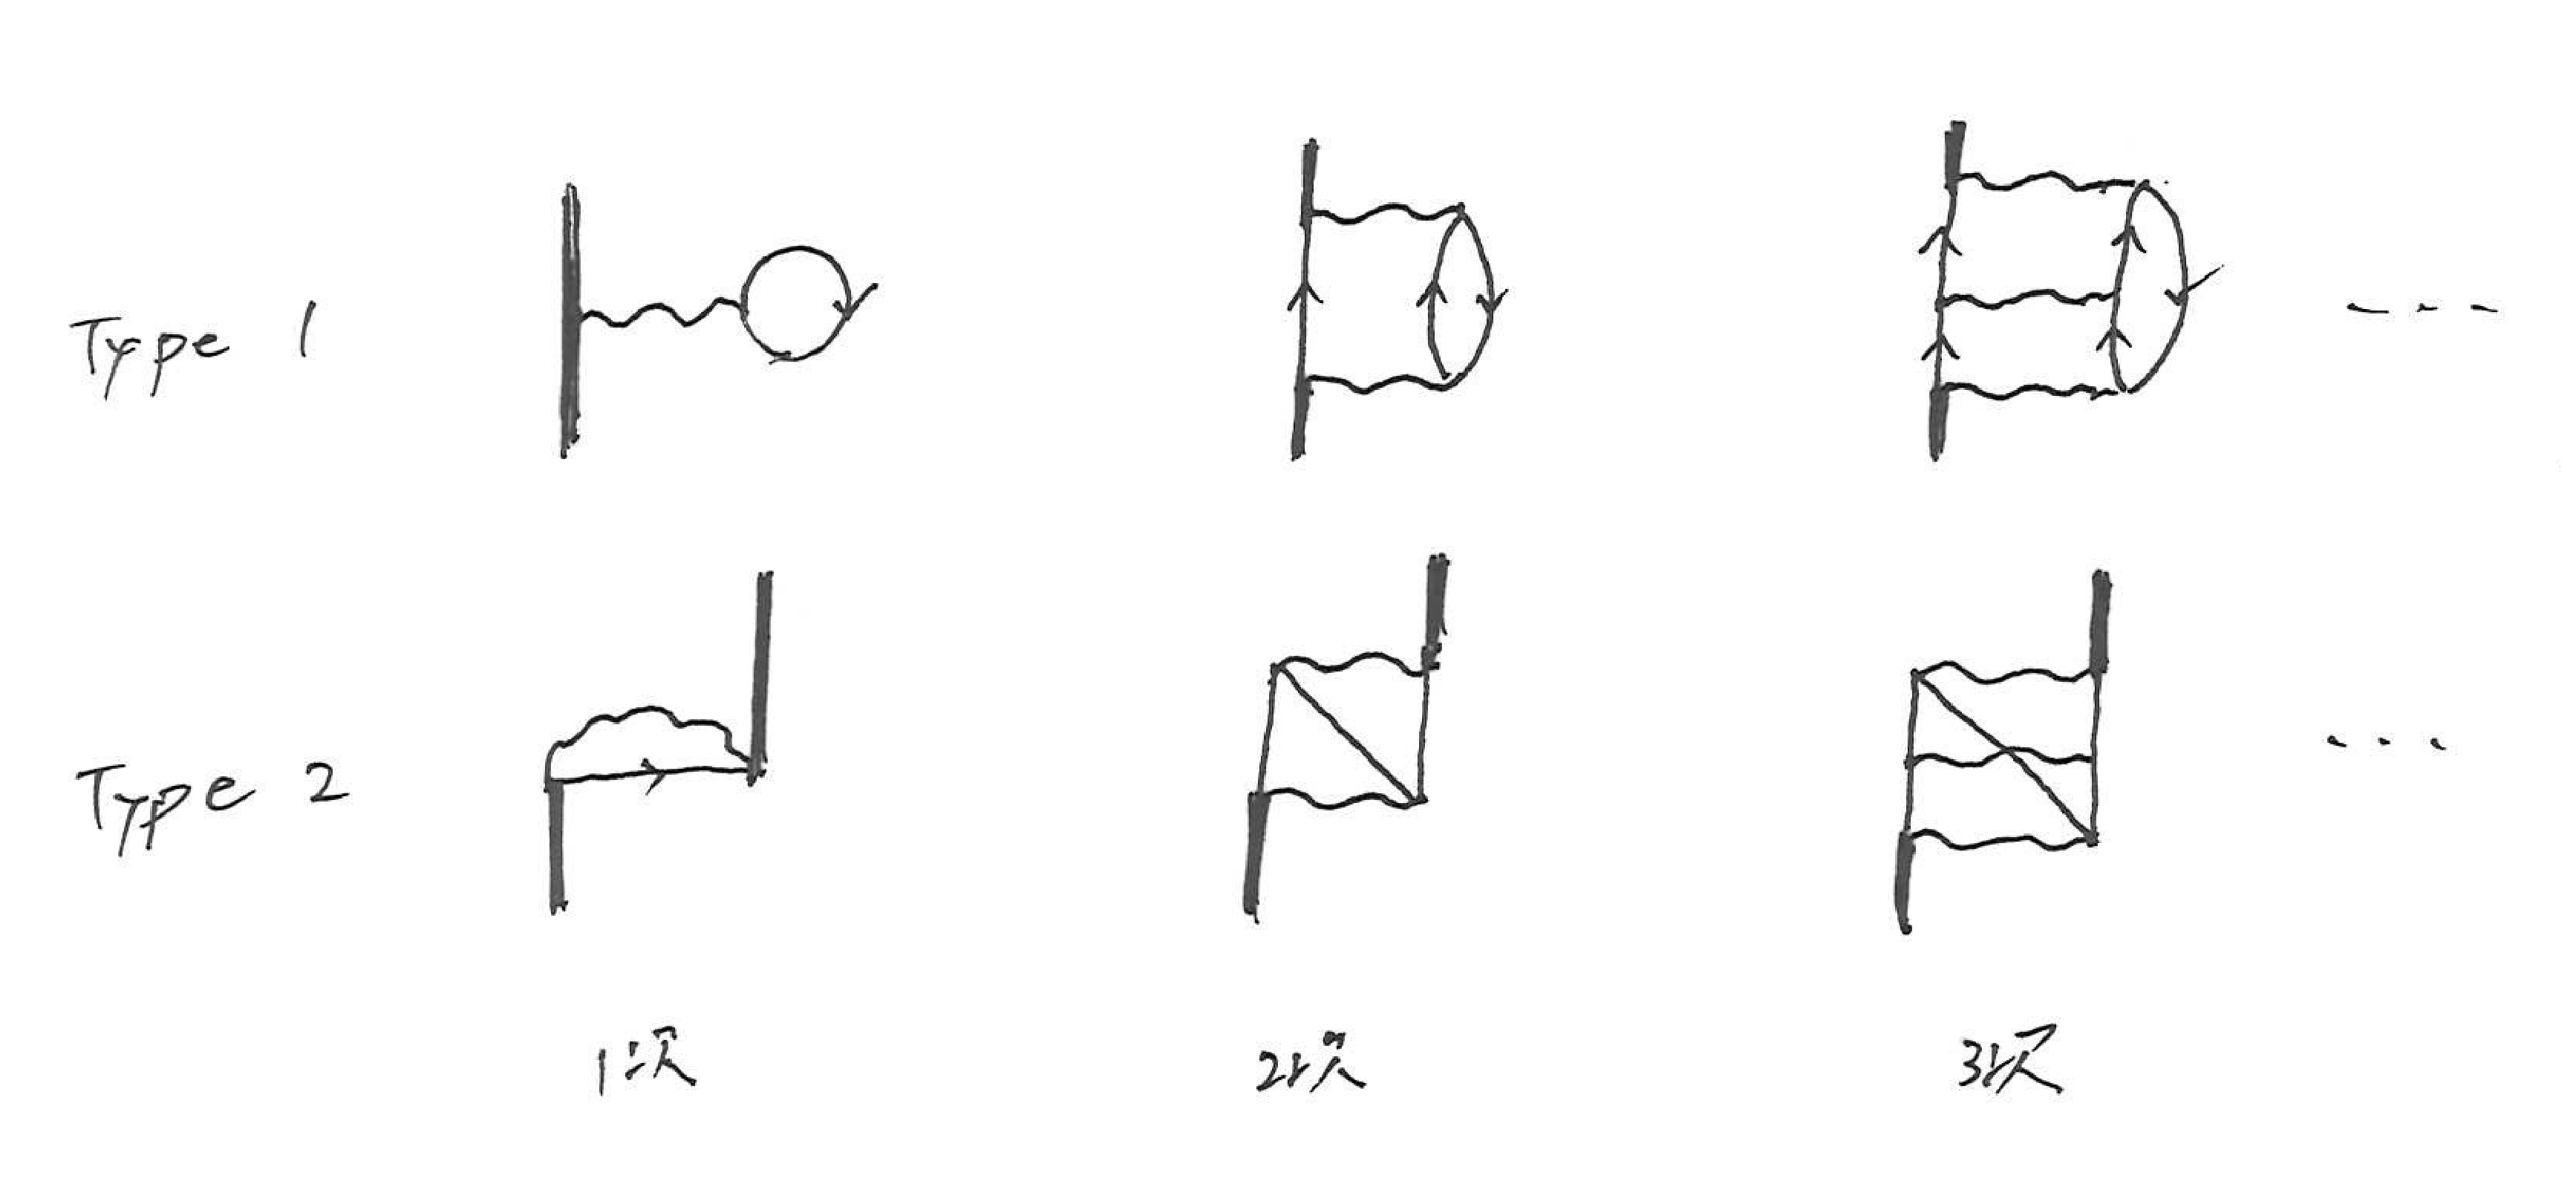
\includegraphics[width = 10cm]{./EPS/ladder1.eps}
  \end{center}
  \caption{梯子近似されたダイアグラム}\label{ladder1}
\end{figure}
太線はFull-Green関数ではなく, $G_0$を表しているので注意. このような梯子型のダイアグラムに限るとき, self-energyは図 \ref{ladder2}のようにまとめることができる.
\begin{figure}[htbp]
  \begin{center}
    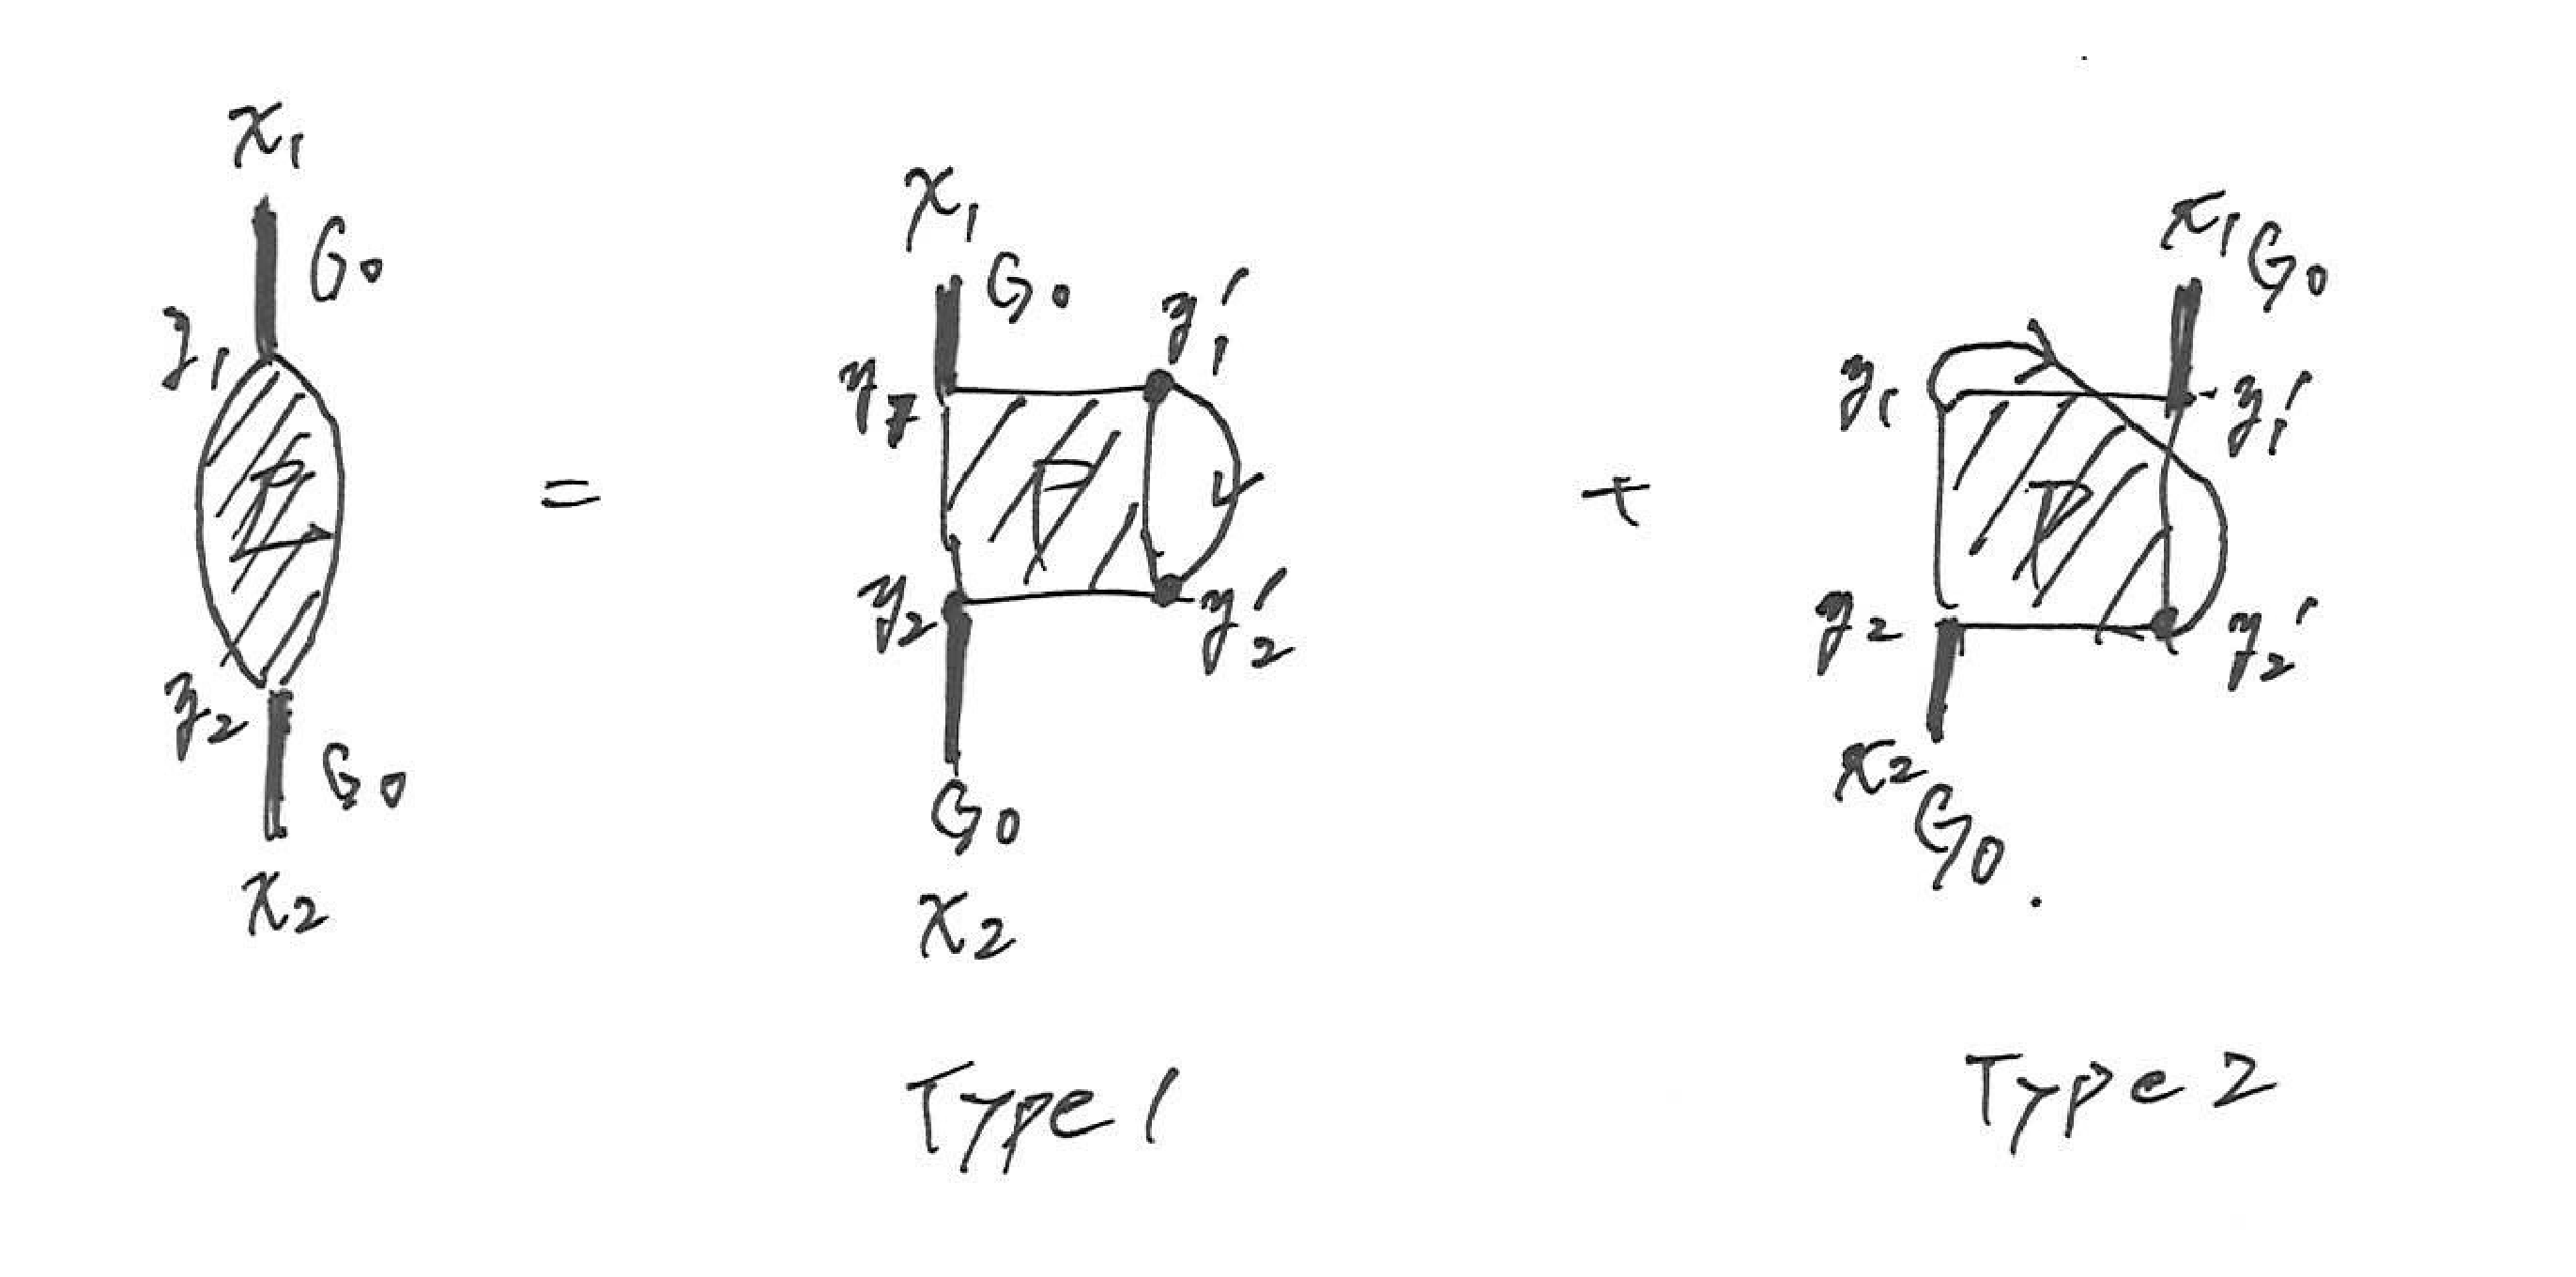
\includegraphics[width = 10cm]{./EPS/ladder2.eps}
  \end{center}
  \caption{梯子近似されたself-energy}\label{ladder2}
\end{figure}
図 \ref{ladder1}のラダーと見比べてみると, $y_i, y'_i$が相互作用していることがわかるが, 今は接触型相互作用を考えているので$y_i' = y_i$としてよい. このとき, self-energyについてType1とType2は全く同じものになる.  さらにType1とType2について$\Gamma$が共通であることが重要(図 \ref{ladder3}).
\begin{figure}[htbp]
  \begin{center}
    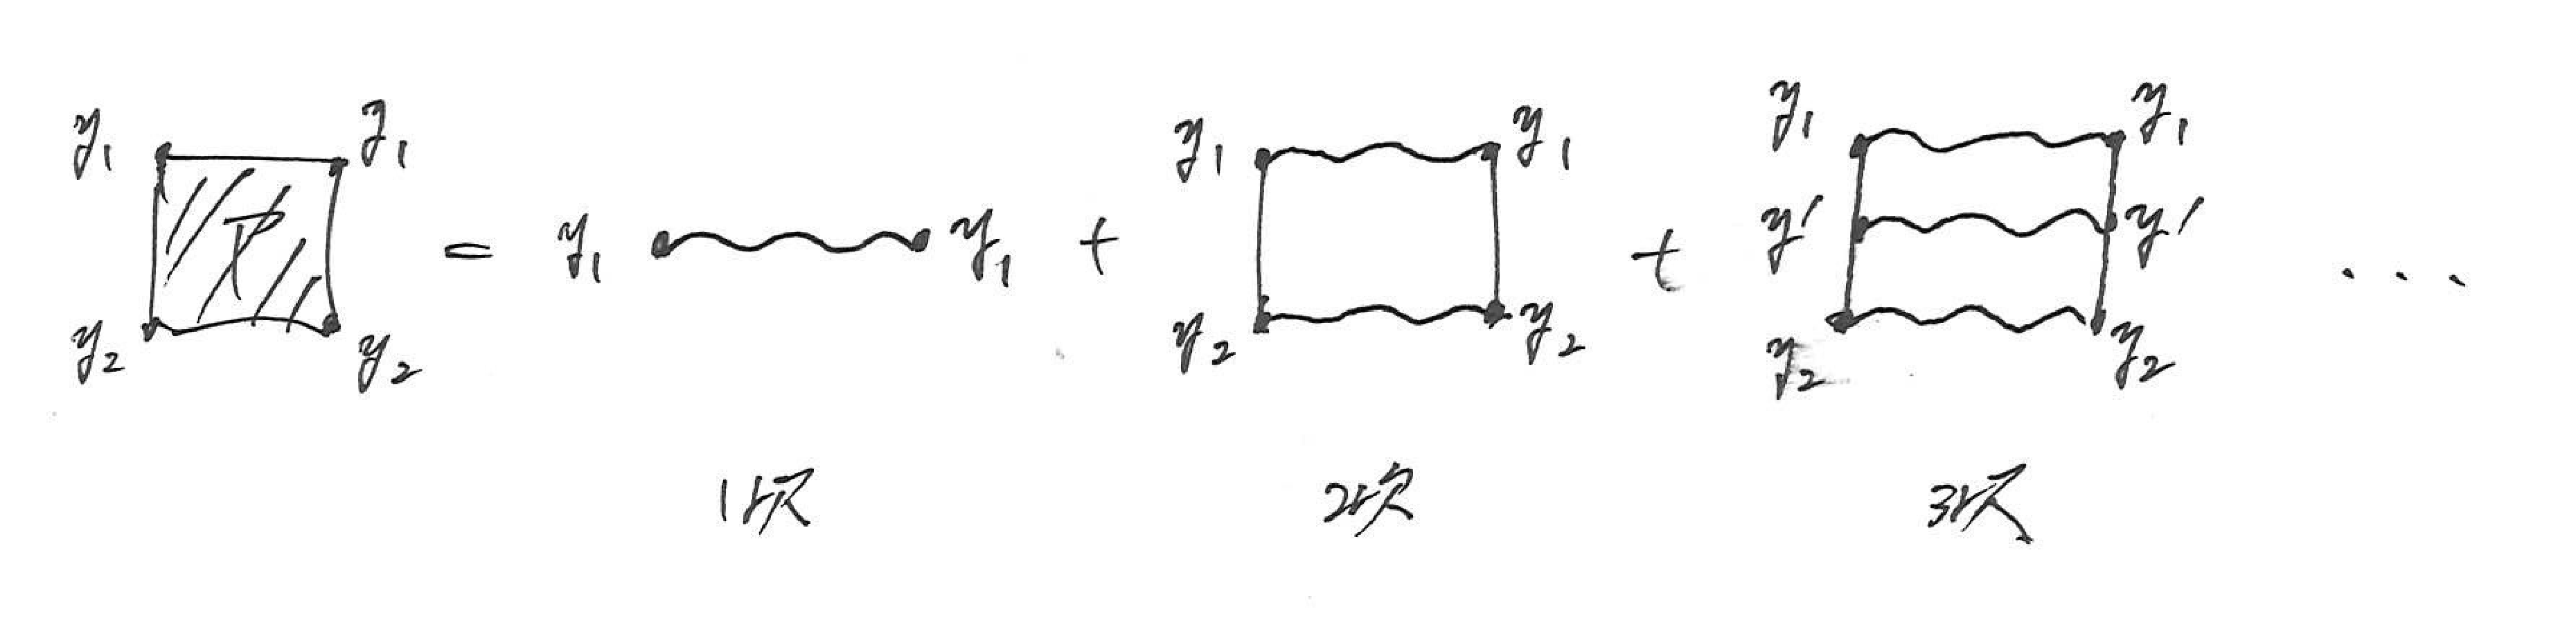
\includegraphics[width = 11cm]{./EPS/ladder3.eps}
  \end{center}
  \caption{$\Gamma$が含むダイアグラム}\label{ladder3}
\end{figure}
さて, 以上のダイアグラムを参考に$G, \Sigma, \Gamma$についての方程式を書き下していく. 今回は簡単のため異常伝搬を含まない1成分のGreen関数について考えることにする. Dyson方程式は
\begin{eqnarray}
  G(x_1, x_2) = G_0(x_1, x_2) + \int d^4y_1d^4y_2\;G_0(x_1, y_1)\Sigma^\star(y_1, y_2)G(y_2, x_2)\label{Ladder-Dyson}
\end{eqnarray}
でありproper self-energyは先ほどのダイアグラムから
\begin{eqnarray}
  \Sigma^\star(y_1, y_2) = 2\Gamma(y_1, y_2)G_0(y_2, y_1)
\end{eqnarray}
のように書くことができる. さらに$\Gamma$は
\begin{eqnarray}
  \nonumber  \Gamma(y_1, y_2) &=& \frac{-ig}{2}\delta(y_1 - y_2) + \qty(\frac{-ig}{2})^2G_0^2(y_1, y_2)\\
  \nonumber  &&+ \qty(\frac{-ig}{2})^3\int dy' G_0^2(y_1, y')G_0^2(y', y_2)\\
  &&+ \qty(\frac{-ig}{2})^4\int dy'dy'' G_0^2(y_1, y')G(y', y'')G_0^2(y'', y_2) + \cdots
\end{eqnarray}
のような無限級数になるが, これは以下のような積分方程式に書きなおすことができる:
\begin{eqnarray}
  \Gamma(y_1, y_2) = \frac{-ig}{2}\delta(y_1 - y_2) + \frac{-ig}{2}\int dy'G_0^2(y_1, y')\Gamma(y', y_2)\label{Bethe-Salpeter}
\end{eqnarray}
これが梯子近似されたBethe-Salpeter方程式と呼ばれるもの. この積分方程式はラダーダイアグラムを無限次取り入れたものになっている. この方程式群は(ラダー近似された)Full-Green関数と$\Gamma$について二重の積分方程式になっている\footnote{さすがにこれは計算が大変そうなので, (\ref{Ladder-Dyson})は一次までにするのが現実的か?}. 非一様系なのでFourier変換ができず, 解析解を求めることは多分できない. ただ, 場の展開をまだ一切用いていないのでもう少し先に進める可能性はあるが, いずれどこかで近似をするなり数値計算に投げるなりは必要になるだろう\footnote{積分方程式の数値計算のノウハウはTFD屋さん(桑原さん・北原)あたりが持っていそう. }. 
\subsection{異常伝搬を含むBethe-Salpeter方程式}
\textbf{(以下, Wickの定理に起因するGreen関数の係数に関する議論が非常に曖昧になります. とりあえずは定式化を優先することにしますが, 係数について後々慎重に議論する必要があります. )}

さて, (\ref{Bethe-Salpeter})を$2\times 2$に拡張する. 素直に以下のような拡張を考えてみることにする:
\begin{eqnarray}
  G^{\mu\nu}(x_1, x_2) &=& G_0^{\mu\nu}(x_1, x_2) + \int d^4y_1d^4y_2\;G_0^{\mu\mu'}(x_1, y_1)\Sigma^{\mu'\nu'}(y_1, y_2)G^{\nu'\nu}(y_2, x_2)\\
  \Sigma^{\star, \mu'\nu'}(y_1, y_2) &=& 2\Gamma^{\mu'\lambda}(y_1, y_2)G_0^{\lambda\nu'}(y_2, y_1)\\
  \Gamma^{\mu'\lambda}(y_1, y_2) &=& \frac{-ig}{2}\delta^{\mu'\lambda}(y_1 - y_2) + \frac{-ig}{2}\int dy'G_0^{\mu'\lambda', 2}(y_1, y')\Gamma^{\lambda', \lambda}(y', y_2)
\end{eqnarray}
これが(\ref{1st-self-energy})を再現しているかどうかを調べる:
\begin{eqnarray}
  G^{22}_1(x, x) &=& \int d^4y_1d^4y_2\;G_0^{2\mu'}(x, y_1)\Sigma_1^{\star, \mu'\nu'}(y_1, y_2)G_0^{\nu'2}(y_2, x)\\
  &=&  2\int d^4y_1d^4y_2\;G_0^{2\mu'}(x, y_1)\Gamma^{\mu'\lambda}(y_1, y_2)G_0^{\lambda\nu'}(y_2, y_1)G_0^{\nu'2}(y_2, x)\\
  &=& -ig\int d^4y_1d^4y_2\;G_0^{2\mu'}(x, y_1)\delta^{\mu'\lambda}(y_1 - y_2)G_0^{\lambda\nu'}(y_2, y_1)G_0^{\nu'2}(y_2, x)
\end{eqnarray}
具体的に書き下すと
\begin{eqnarray}
  G^{22}_1(x, x) &=& -ig\int d^4y_1d^4y_2\;\Bigl[G_0^{21}(x, y_1)\delta(y_1 - y_2)G_0^{11}(y_2, y_1)G_0^{12}(y_2, x)\\
    && \hspace{2.5cm} + G_0^{22}(x, y_1)\delta(y_1 - y_2)G_0^{21}(y_2, y_1)G_0^{12}(y_2, x)\\
    && \hspace{2.5cm} + G_0^{21}(x, y_1)\delta(y_1 - y_2)G_0^{12}(y_2, y_1)G_0^{22}(y_2, x)\\
    && \hspace{2.5cm} + G_0^{22}(x, y_1)\delta(y_1 - y_2)G_0^{22}(y_2, y_1)G_0^{22}(y_2, x)\Bigr]
\end{eqnarray}
同時刻Green関数は左側にダガーを持ってくる約束なので$G^{22}(y_2, y_1) = G^{11}(y_2, y_1)$とすることができる. しかしこれでは(\ref{1st-self-energy})と係数が一致していない. 場当たり的にはクロネッカーデルタを
\begin{eqnarray}
  G^{\mu\nu}_1(x, x) &=& -ig(1+\delta_{\mu'\nu'})\int d^4y_1d^4y_2\;G_0^{\mu\mu'}(x, y_1)\delta(y_1 - y_2)G_0^{\mu'\nu'}(y_2, y_1)G_0^{\nu'\nu}(y_2, x)
\end{eqnarray}
のように追加すれば一致するが, 2次以上を考えても本当にこれでいいのか\footnote{そもそも今はラダーダイアグラムしか拾ってこない近似をしているので, 2次以上ではそもそも一致することはないので深く考えすぎなくてもよいかも. が, 1次については当然一致しなければならない. }・これを元の方程式のどこに追加すればよいかなどはよく考えなければならない\footnote{そもそも計算が合ってるのかも不安ではある. 2次以上もやってみるのがいいんだろうが, とてもめんどくさい. self-energyの対角成分と非体育成分ではそもそも係数の付け方の規則が違うとかの可能性もある?}.

...考え中...
\subsection{摂動ハミルトニアン3次の取り扱い}
摂動ハミルトニアンには3次の項もあった. これは摂動1次には現れてこないが, 2次以降はその限りではなく, かつ3次の項は秩序変数を含むためその寄与も大きいのではないかと考えられる\footnote{粒子が十分に凝縮している領域を考えると$\xi$が効いてくるから, という単純な理由. もちろん, c-数である$\xi$と演算子の$\varphi$の大小比較はできないので確実に効いてくるという根拠は無いが...}. 摂動ハミルトニアンを
\begin{eqnarray}
  \nonumber  H_{\rm int} &=& g\int d\bx \qty(\xi \varphi_{\rm ex}^\dagger(x)\varphi_{\rm ex}^\dagger(x)\varphi_{\rm ex}(x) + \xi^*(x)\varphi_{\rm ex}^\dagger(x)\varphi_{\rm ex}(x)\varphi_{\rm ex}(x) + \frac12\varphi_{\rm ex}^\dagger(x)\varphi_{\rm ex}^\dagger(x)\varphi_{\rm ex}(x)\varphi_{\rm ex}(x))\\
  &=& {\cal H}_3 + {\cal H}_3^\d + {\cal H}_4
\end{eqnarray}
と置いたときGreen関数の摂動2次の展開は以下の通り:
\begin{eqnarray}
  \nonumber  G_2^{22}(x, x) &=& (-i)^2\int ds_1ds_2\ev{T\qty[H_{\rm int}(s_1)H_{\rm int}(s_2)\varphi^\d(x)\varphi(x)]}\\
  &=& (-i)^2\int ds_1ds_2\ev{T\qty[{\cal H}_4(s_1){\cal H}_4(s_2)\varphi^\d(x)\varphi(x)]}\\
  &&\hspace{2.0cm} + \ev{T\qty[{\cal H}_3(s_1){\cal H}_3(s_2)\varphi^\d(x)\varphi(x)]}\label{2nd-Green-first}\\
  &&\hspace{2.0cm} + \ev{T\qty[{\cal H}_3(s_1){\cal H}^\d_3(s_2)\varphi^\d(x)\varphi(x)]}\\
  &&\hspace{2.0cm} + \ev{T\qty[{\cal H}^\d_3(s_1){\cal H}_3(s_2)\varphi^\d(x)\varphi(x)]}\\
  &&\hspace{2.0cm} + \ev{T\qty[{\cal H}^\d_3(s_1){\cal H}^\d_3(s_2)\varphi^\d(x)\varphi(x)]}\label{2nd-Green-final}
\end{eqnarray}
${\cal H}_4$の項は既に前節の梯子近似されたBethe-Salpeter方程式に組み込まれている. ${\cal H}_3$が2つ連結された項4つの項は図(\ref{ladder3-5})のようなダイアグラムになる. 
\begin{figure}[H]
  \begin{center}
    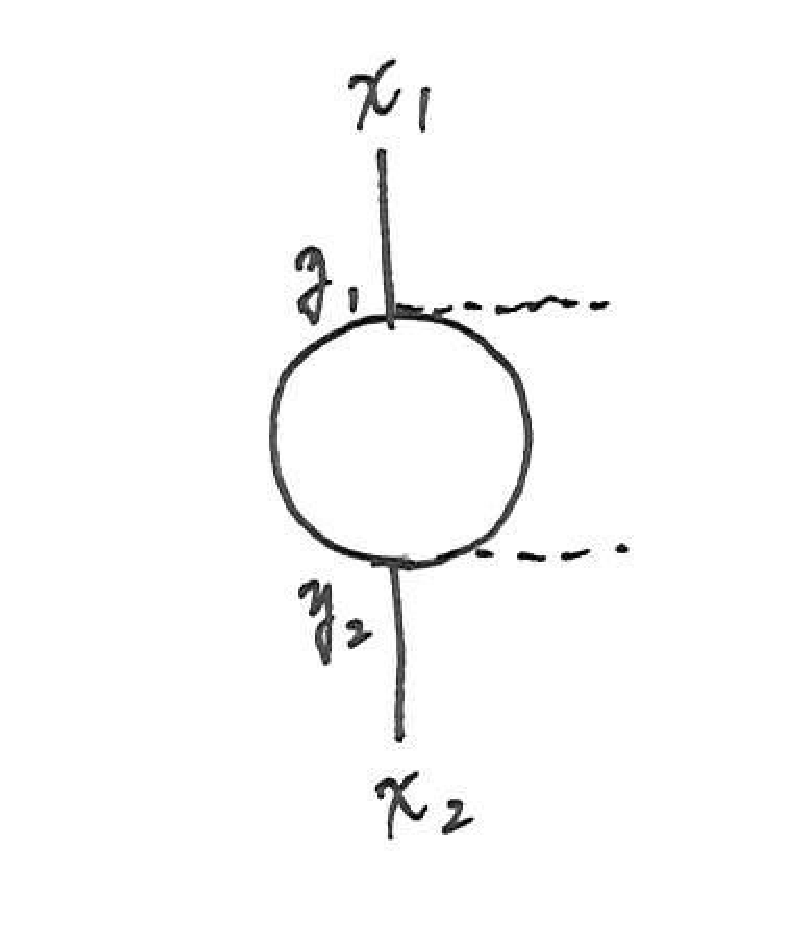
\includegraphics[width = 3cm]{./EPS/ladder3-5.eps}
  \end{center}
  \caption{${\cal H}_3$が2つ連結されたダイアグラム}\label{ladder3-5}
\end{figure}
破線は凝縮線で, 秩序変数$\xi$に対応している. さて, 上のような${\cal H}_3$を含むダイアグラムをどのように集めてくるかが重要になるが, 今回も前節に倣ってラダーダイアグラムを引っ張ってくることにする. 3次を含むラダーダイアグラムは例えば以下の通り:
\begin{figure}[H]
  \begin{center}
    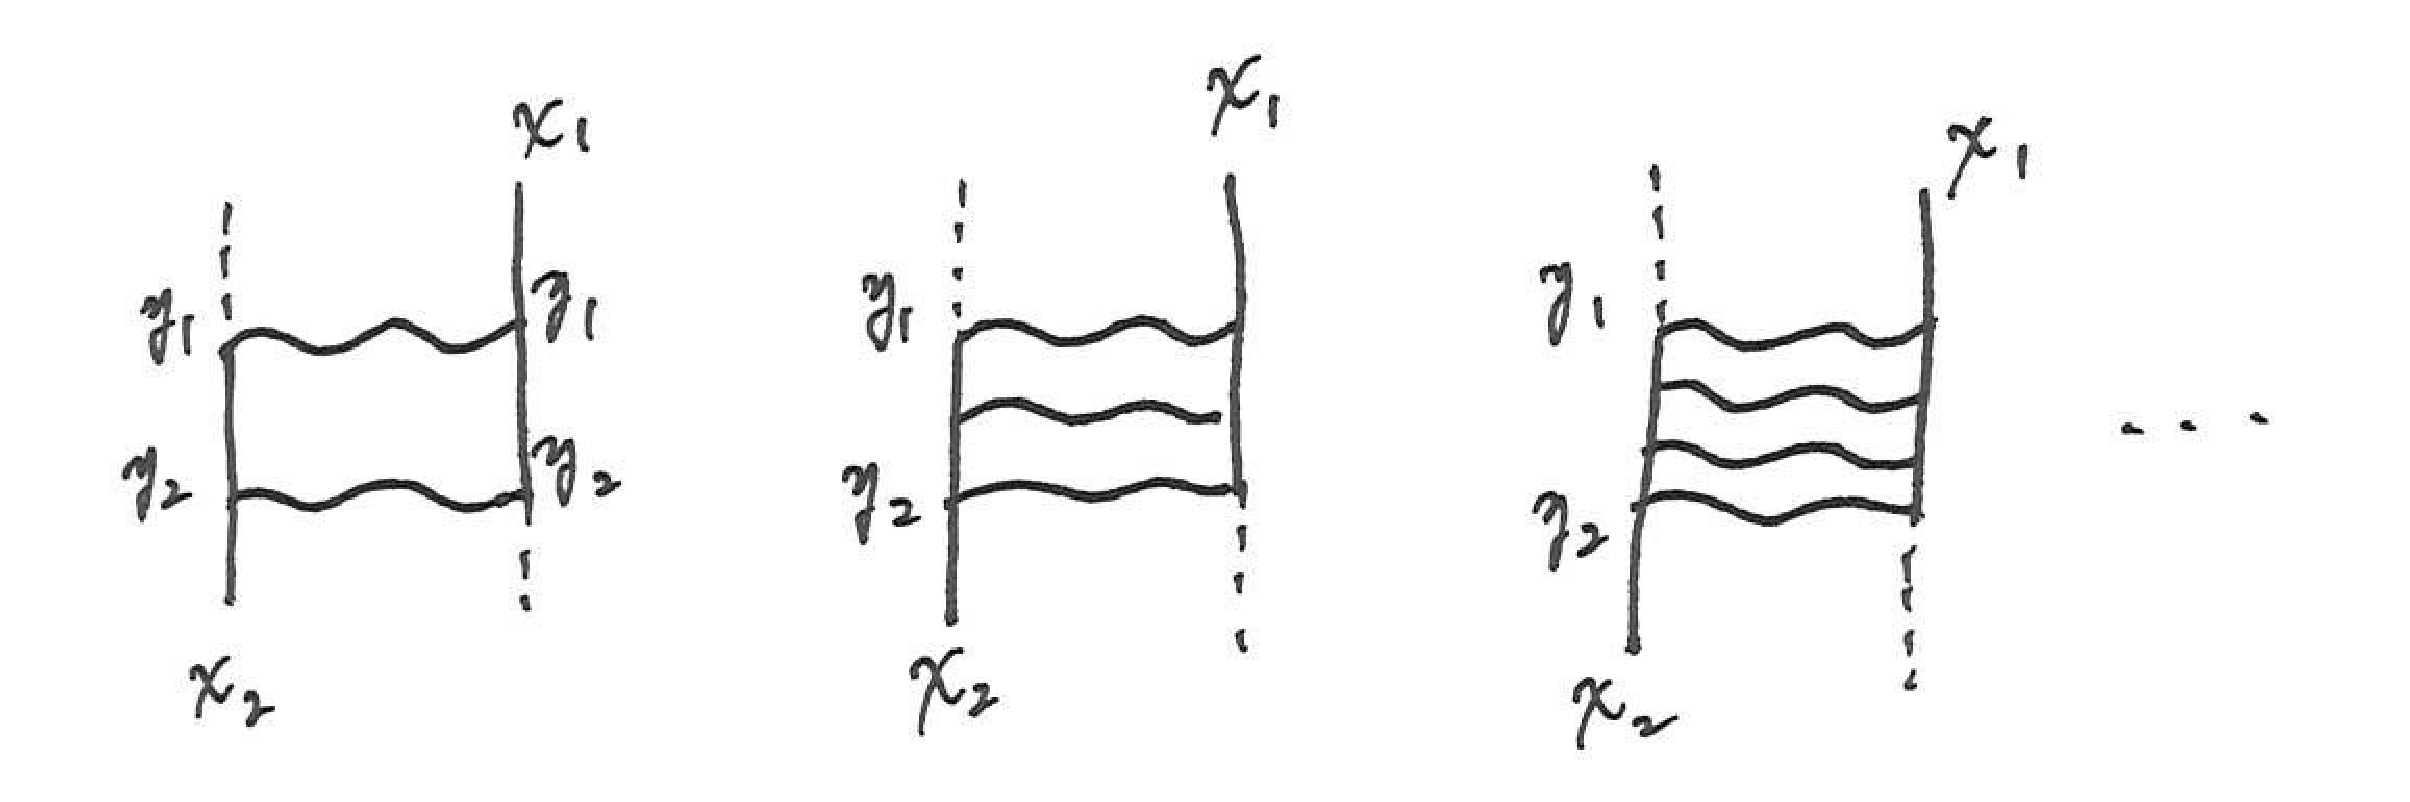
\includegraphics[width = 8cm]{./EPS/ladder3-1.eps}
  \end{center}
\end{figure}
これは2つの${\cal H}_3$の間に${\cal H}_4$が挿入されているようなダイアグラムを拾っていることに対応する\footnote{${\cal H}_3$は端に2つあるだけで, 結局ラダーの元になっているのは${\cal H}_4$である. これで${\cal H}_3$の寄与を十分に取り入れることができているかは不明. ${\cal H}_3$のみで構成されるようなproperなダイアグラムが効いてくるなら, それをFull-orderで取り入れるのが理想だが, そのような定式化はまだできていない. 出来るかどうかも勉強してみなければわからない. }. これは前節同様$\Gamma$を用いて表すことができそうである:
\begin{figure}[H]
  \begin{center}
    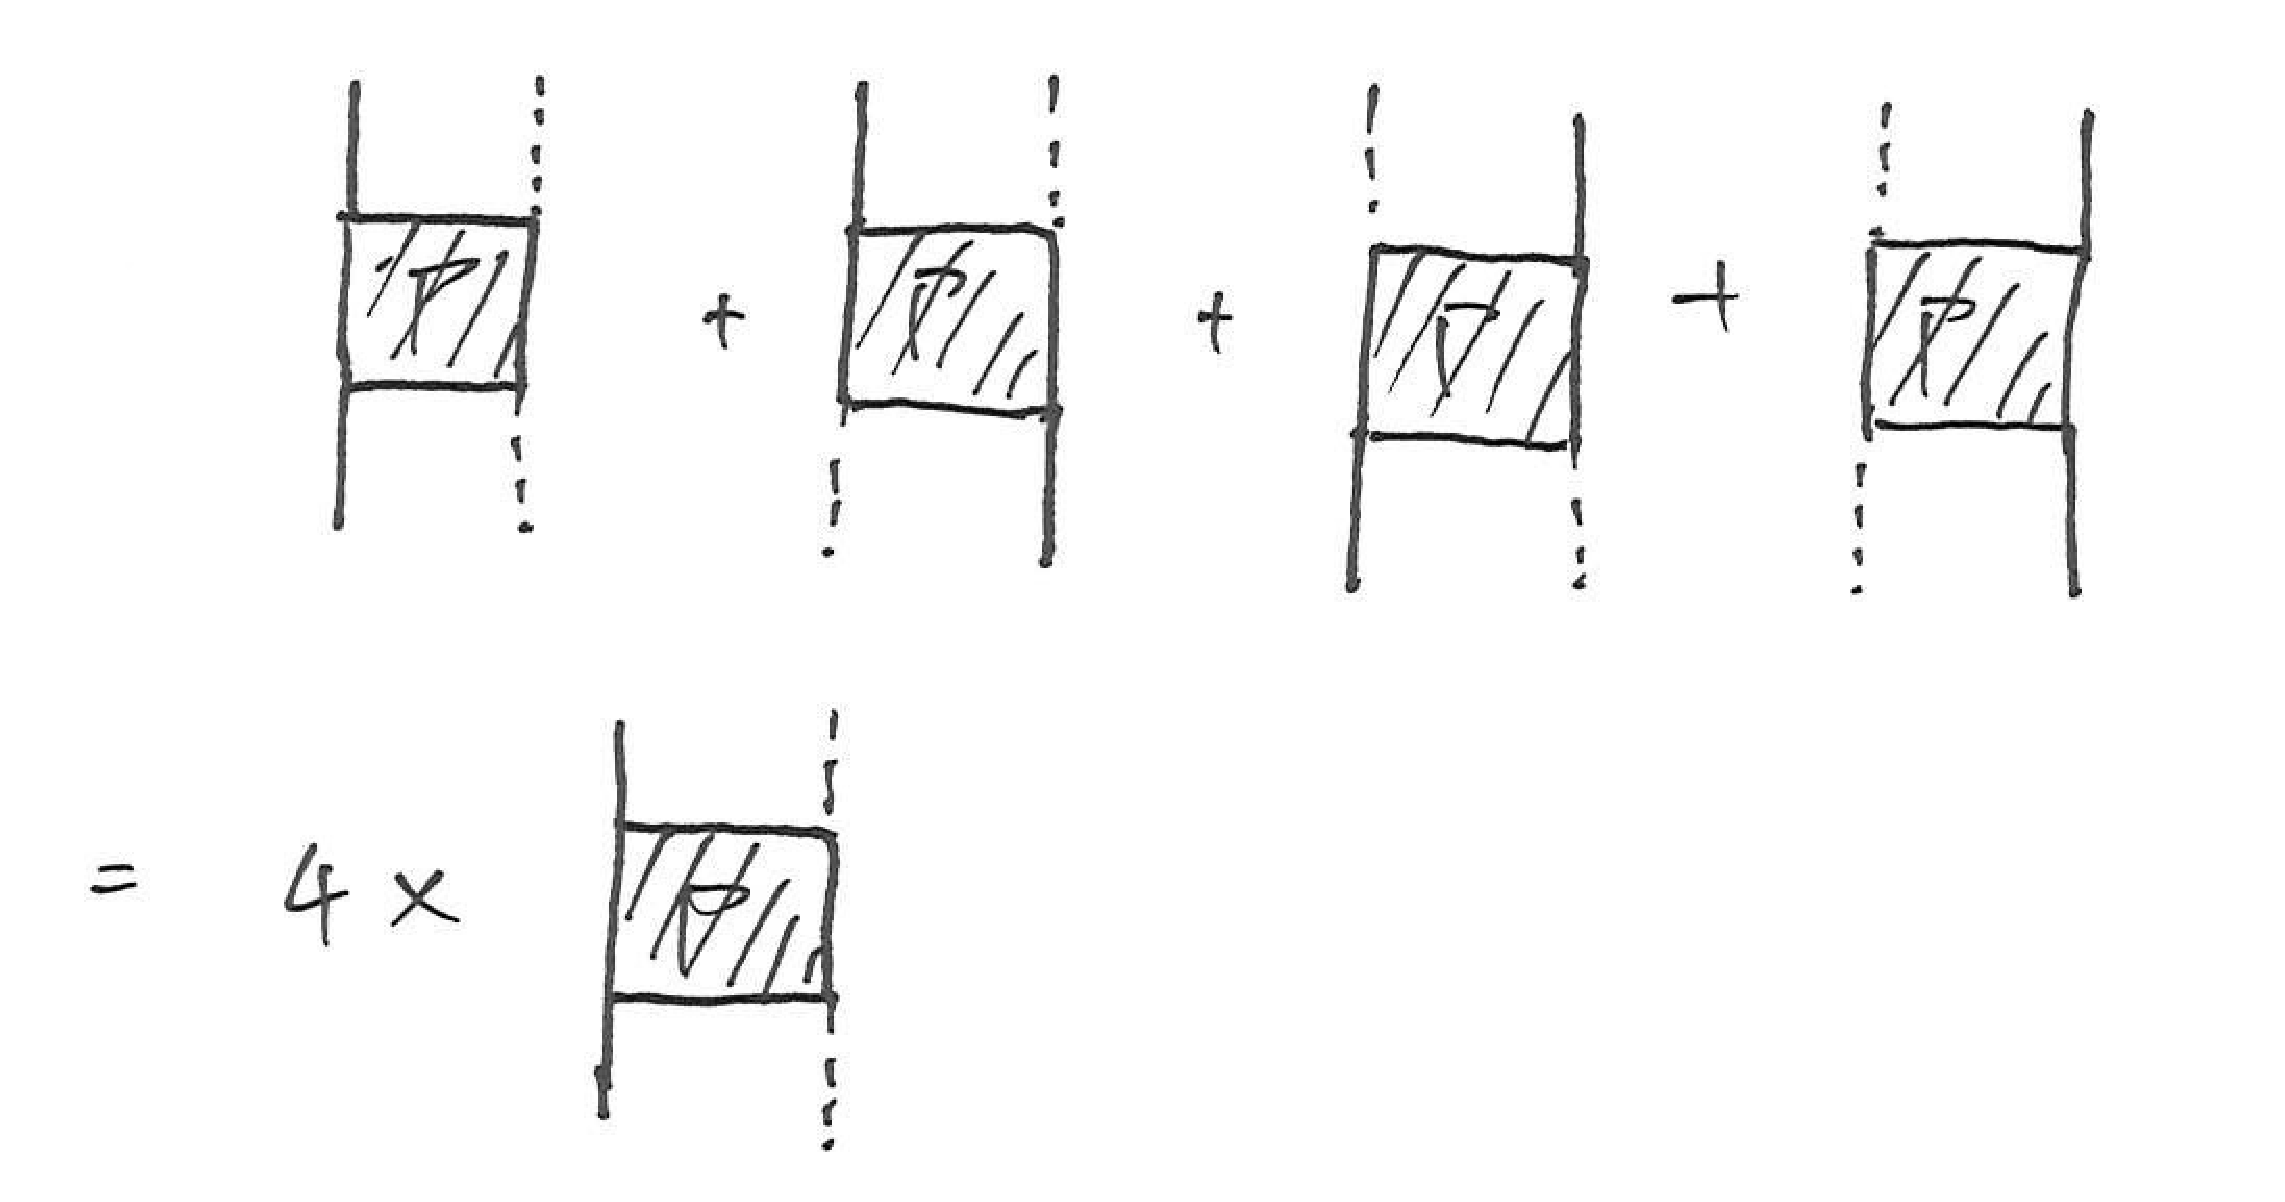
\includegraphics[width = 8cm]{./EPS/ladder3-2.eps}
  \end{center}
\end{figure}
しかしながら, $\Gamma(y_1, y_2)$は$\delta(y_1 - y_2)$を含んでおり, これに対応する展開$\xi(y_1)\xi^*(y_1)\delta(y_1 - y_2)G_0(x_1, y_1)G_0(y_2, x_2)$が摂動2次に現れないことは明らか. ということで, この現れない項を$\Gamma$から引いてこれをself-energyとする:
\begin{figure}[H]
  \begin{center}
    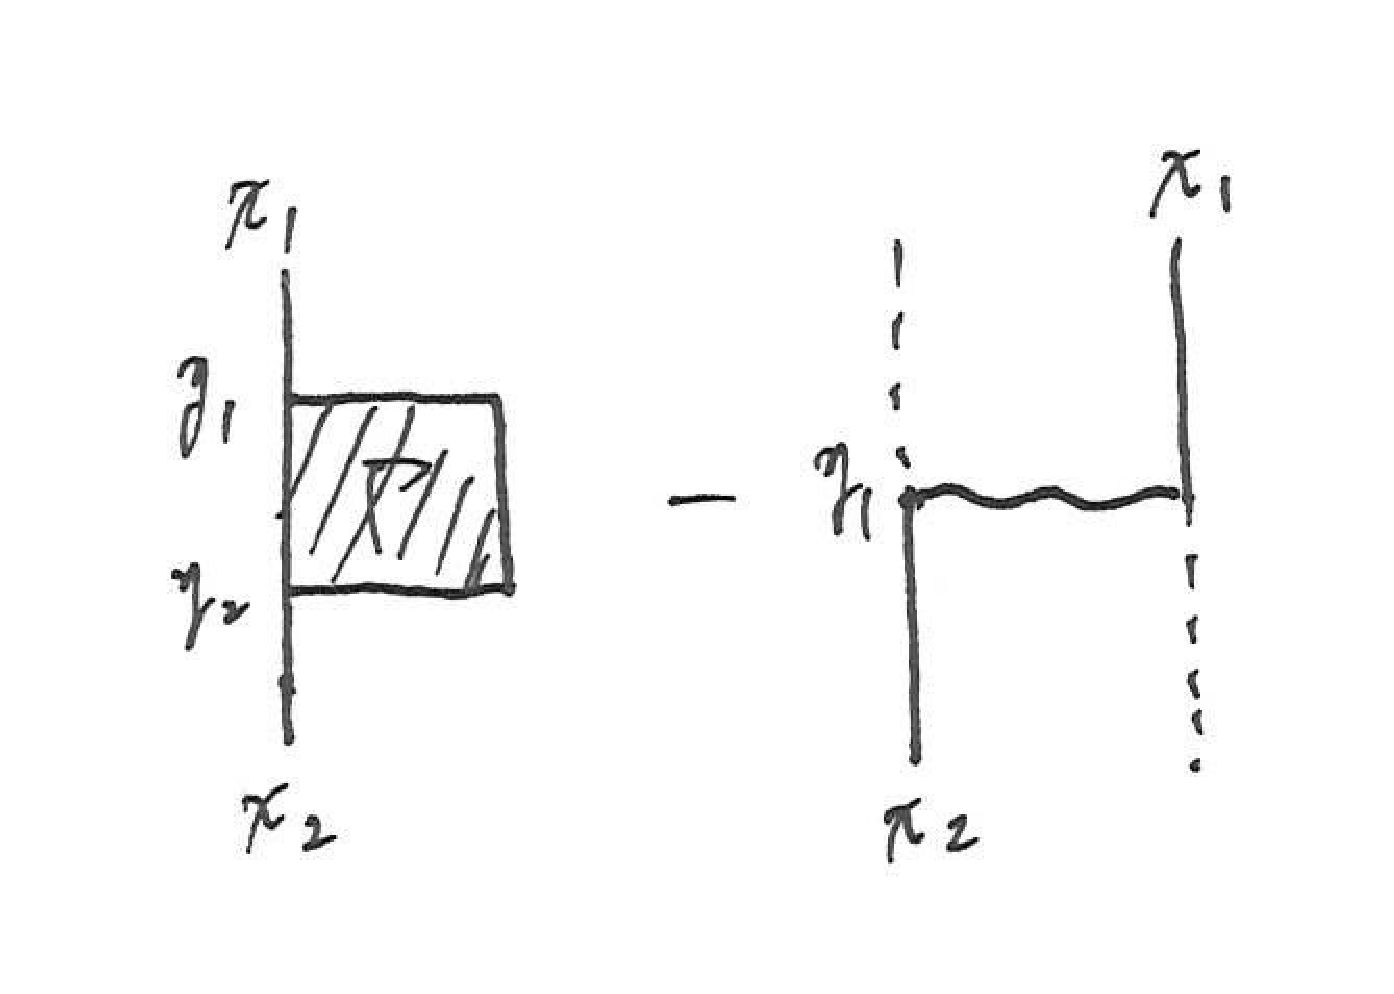
\includegraphics[width = 5.5cm]{./EPS/ladder3-4.eps}
  \end{center}
\end{figure}
ここまでくれば, あとは$\xi$が複素共役になるか否かについての規則を考える. Green関数の2次の展開について(\ref{2nd-Green-first})-(\ref{2nd-Green-final})についてのダイアグラムは以下の通り:
\begin{figure}[H]
  \begin{center}
    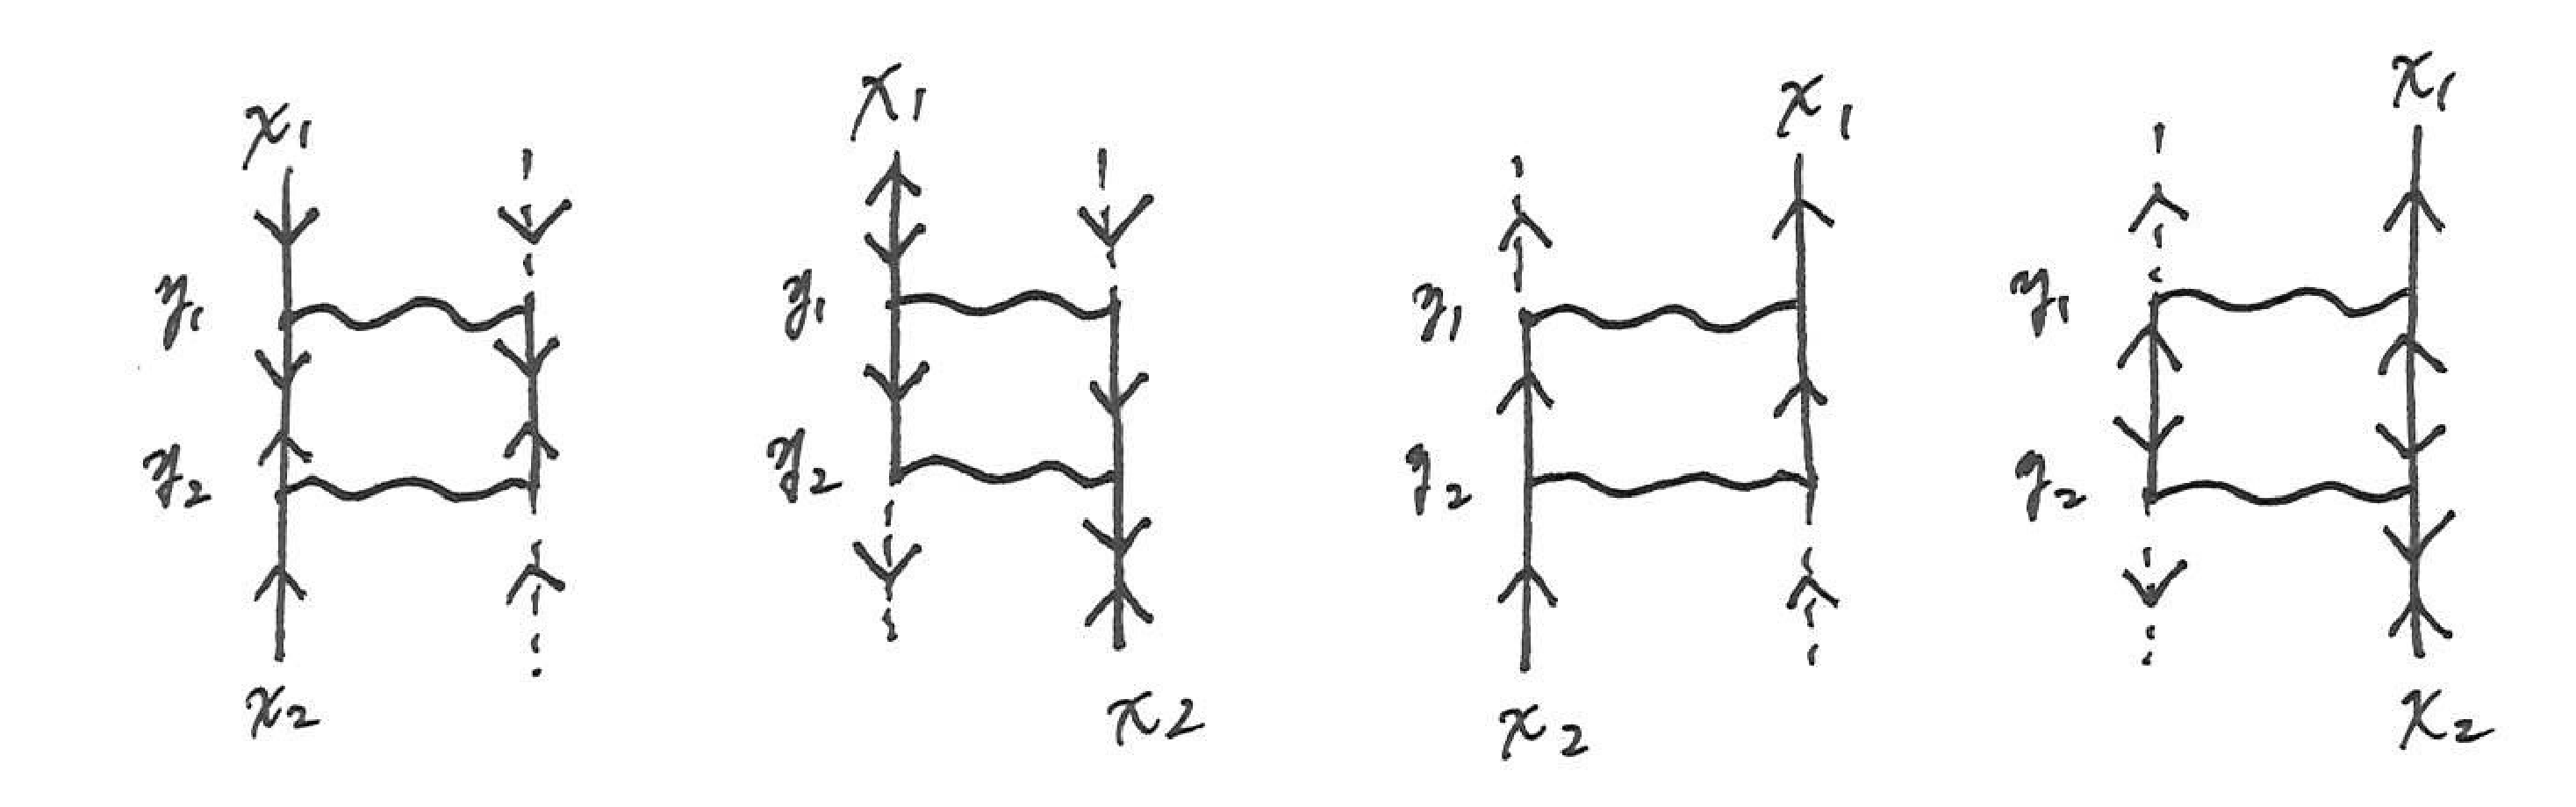
\includegraphics[width = 10cm]{./EPS/ladder3-3.eps}
  \end{center}
\end{figure}
凝縮線の向きは$\Gamma(y_1, y_2)$に接続されたGreen関数の$y_1, y_2$成分の向きと同じであり, つまり$\mu', \nu'$に依存しているということである. $\xi$の向きに応じて展開係数が変化することはないことがわかる. このことから, 3次のダイアグラムを加味したself-energyは
\begin{eqnarray}
  \Sigma^{\star, \mu'\nu'}(y_1, y_2) &=& 2\Gamma^{\mu'\lambda}(y_1, y_2)G_0^{\lambda\nu'}(y_2, y_1) + 4\Xi^{\mu'\nu'}\qty[\Gamma^{\mu'\nu'}(y_1, y_2) + \frac{ig}{2}\delta^{\mu'\nu'}(y_1 - y_2)]\\
  \Xi^{\mu'\nu'}&=&
  \begin{bmatrix}
    \xi^*(y_1)\xi(y_2)&\xi^*(y_1)\xi^*(y_2)\\
    \xi(y_1)\xi(y_2)&\xi(y_1)\xi^*(y_2)
  \end{bmatrix}^{\mu'\nu'}
\end{eqnarray}
いずれ具体計算の際に$\xi$が実であることを仮定するので, その仮定の下ではもう少しシンプルになる:
\begin{eqnarray}
  \Sigma^{\star, \mu'\nu'}(y_1, y_2) &=& 2\Gamma^{\mu'\lambda}(y_1, y_2)G_0^{\lambda\nu'}(y_2, y_1) + 4\xi(y_1)\xi(y_2)\qty[\Gamma^{\mu'\nu'}(y_1, y_2) + \frac{ig}{2}\delta^{\mu'\nu'}(y_1 - y_2)]
\end{eqnarray}

\subsection{実効的な計算が可能な形へ...は難しい}
山中先生との議論の結果, ナイーブにGreen関数を計算するのはムリなのでは?ということに. 方向転換. 
\subsection{ゼロモードハミルトニアンの平均場的な取り扱い(暫定版)}
ゼロモードを摂動的に取り入れることが困難であるので, 摂動的に扱うべき(\ref{ZeromodeHamiltonian})についてはゼロモード期待値を取ってc-数にしてしまうことにする:
\begin{eqnarray}
  \nonumber  \ev{H_{\rm int}}_{\rm z} &=& \int d\bm{x} \Bigl[g\xi^*(2\ev{\varphi_z^\dagger\varphi_z}_{\rm z}\varphi_{ex} + \ev{\varphi_z\varphi_z}_{\rm z}\varphi_{ex}^\dagger)\\
    \nonumber  && +\ g\xi\ (2\ev{\varphi_z^\dagger\varphi_z}_{\rm z}\varphi_{ex}^\dagger + \ev{\varphi_z^\dagger\varphi_z^\dagger}_{\rm z}\varphi_{ex})\\
    \nonumber  && +\ g(\ev{\varphi^\dagger_z\varphi^\dagger_z\varphi_z}_{\rm z}\varphi_{ex} + \ev{\varphi^\dagger_z\varphi_z\varphi_z}_{\rm z}\varphi^\dagger_{ex}) \\
    && +\ \frac{g}{2}\qty(\ev{\varphi^\dagger_z \varphi^\dagger_z}_{\rm z} \varphi_{ex}\varphi_{ex} + 4\ev{\varphi^\dagger_z \varphi_z}_{\rm z} \varphi^\dagger_{ex}\varphi_{ex} + \ev{\varphi_z \varphi_z}_{\rm z} \varphi^\dagger_{ex}\varphi^\dagger_{ex})\Bigr]\label{ZeromodeHamiltonian2}
\end{eqnarray}
ゼロモードの一次は期待値を取ると消えることを利用している. これはもう励起モードの1次・2次になっているので非摂動ハミルトニアンに取り入れるのが妥当だと考えられる. その前に, ゼロモード期待値についてまとめておく(ここでも$\xi$が実であることを仮定):
\begin{eqnarray}
  \nonumber  \ev{\varphi^\dagger_z\varphi^\dagger_z}_z &=& V_a^0 = \ev{(-i\xi Q + \eta P)^\dagger(-i\xi Q + \eta P)^\dagger}_z = -\xi^2\ev{Q^2}_z + \eta^2\ev{P^2}_z\\
  \nonumber \ev{\varphi_z^\dagger\varphi_z}_z &=&  V_t^0 = \xi^2\ev{Q^2}_z + \eta^2\ev{P^2}_z - i\xi\eta\\
  \nonumber \ev{\varphi_z\varphi_z}_z &=& V_a^0 =  -\xi^2\ev{Q^2}_z + \eta^2\ev{P^2}_z\\
  \ev{\varphi_z^\d\varphi_z^\d\varphi_z}_z &=& \ev{\varphi_z^\d\varphi_z\varphi_z}_z = R_3 = \xi^2\eta \ev{QPQ}_z + \eta^3\ev{P^3}_z\label{Zeromode-Exp2}
\end{eqnarray}
さて, (\ref{ZeromodeHamiltonian2})を非摂動ハミルトニアンに組み込むと以下のようになる:
\begin{eqnarray}
  H_{\rm u, 1} &=& \int d\bx\Bigl[\varphi_{\ex}\qty{h_0 -\mu + g(|\xi|^2 + 2V_t^0 + V_a^0)}\xi + {\rm h.c.}\Bigr]\\
  H_{\rm u, 2} &=& \int d\bx\qty[\varphi_{\ex}^\d\calL\varphi_{\ex} + \frac12\varphi_{\ex}\calM'^{*}\varphi_{\ex} + \frac12\varphi_{\ex}^\d\calM'\varphi_{\ex}^\d]\\
  \calL' &=& h_0 - \mu +2g(|\xi|^2 + V_t^0),\hspace{0.7cm}\calM' = g(|\xi|^2 + V_a^0)
\end{eqnarray}
これは有限温度ゼロモードの論文[arXiv:1604.05900]の式(8)-(10)にゼロモード期待値という意味でほぼ対応している. 本来の量子補正は$\calM = g\qty(|\xi|^2 - V_a)$なので符号が異なる. こうなってないとゼロモード解が壊れてしまうので, 繰り込みで守るようにしなければならない\footnote{元の理論とすこし違う形の繰り込みになってしまうかもしれないが, 恐らくうまく行くと思う. }. 

まだしっかりformulateしたわけではないが, 相互作用ハミルトニアンのゼロモード平均場を非摂動部に取り込むということは, 量子補正$\ev{\varphi^\d_{\rm H}\varphi_{\rm H}}, \ev{\varphi_{\rm H}\varphi_{\rm H}}$についてゼロモード期待値は最低次のみを取ってくることに恐らく対応している. したがって現状の方針においては, 量子補正は励起をall-orderで, ゼロモードは最低次のみを取るのみで(おそらく)十分である\footnote{その励起のall-orderが大変なのですが...}ことがわかった.
\section{方向転換}
あの積分方程式を真面目に計算するのはキツイので, $\Gamma$を量子力学の散乱問題における散乱振幅$f$に置き換える方法で進める. 非一様でエネルギーの表式を求め, 一様近似でLee-Yangのアレと一致するようになれば十分. 大橋研のT-matrix近似についても調査したい.
\section{散乱の量子力学からBethe-Salpeter方程式の置換えへ}
\subsection{Schr\"odinger方程式}
Schr\"odinger方程式
\begin{eqnarray}
  \nabla^2u_k + \qty(k^2 - U(\bm{r}))u_k = 0\hspace{1cm} k^2 = \frac{2mE}{\hbar^2}\label{schroedinger-scatter}
\end{eqnarray}
でポテンシャルが$|\bm{r}U(\bm{r})|\rightarrow 0\ \ (\bm{r}\rightarrow\infty)$を満たすものとする. さて, 境界条件をどうするかを考えなければならないが, 散乱固有関数は十分遠方では入射平面波$u_k^0$と散乱の効果である外向き球面波$u_k^{sc}$の重ね合わせでなければならない. $u_k^{sc}$も(\ref{schroedinger-scatter})を満たすので
\begin{eqnarray}
  u_k^{sc} = \phi_k(r)f(\theta, \varphi)
\end{eqnarray}
という特解を持つはず. 十分遠方ではラプラシアンの$r^{-2}$の項が無視できるので$\phi_k$について
\begin{eqnarray}
  \frac{d^2}{dr^2}(r\phi_k) + k^2(r\phi_k) = 0\hspace{1cm}\therefore\phi_k = \frac{1}{r}\exp(\pm ikr)
\end{eqnarray}
ということで, 境界条件として以下を採用する\footnote{$u_k^-$という条件も考えられるが, 物理的状況に対応していないので今回は用いない. ただし, 計算の道具としては有用らしい. }:
\begin{eqnarray}
  u_k^+\rightarrow \frac{1}{(2\pi)^{\frac32}}\qty(e^{i\bk\cdot\bm{r}} + \frac{1}{r}e^{i\bk\cdot\bm{r}}f(\theta, \varphi))\ \ \ (r\rightarrow \infty)
\end{eqnarray}
Schr\"odinger方程式を上の境界条件の下で解くと$f(\theta, \varphi)$が求まる. Green関数を用いて$u_k^+$に関する積分方程式をつくると
\begin{eqnarray}
  u_k^+\rightarrow \frac{1}{(2\pi)^{\frac32}}\qty(e^{i\bk\cdot\bm{r}} - (2\pi)^{\frac32}\frac{e^{i\bk\cdot\bm{r}}}{4\pi r}\int d\bm{r}'e^{^i\bk'\cdot\bm{r}'}U(\bm{r}')u_k^+(\bm{r}'))\ \ \ (r\rightarrow \infty)\label{scatter-psi}
\end{eqnarray}
となり, 先ほどの境界条件と比較することで$u_k^+$と$f(\theta, \varphi)$の関係を得る.
\subsection{問題意識}
考えなければいけないことは主に3つ:
\begin{itemize}
\item[1.] $\frac{m}{\hbar^2}\Gamma = \tilde{f} + \int\frac{dk}{(2\pi)^3}\tilde{f}\qty(\frac{1}{\epsilon - k^2 + i\eta} + \frac{1}{\epsilon - p'^2 + i\eta})\tilde{f}^*\hspace{0.3cm}(22.3)\hspace{0.3cm}$のように書けること.
\item[2.] 長波長のとき$\Gamma\rightarrow 4\pi a\hbar^2/m$になること. 
\item[3.] $E/V = \frac{2\pi n^2a\hbar^2}{m}\qty[1 + \frac{128}{15}\qty(\frac{na^3}{\pi})^{\frac12}]$になること. 
\end{itemize}
\subsection{$\Gamma_0$が散乱振幅$\tilde{f}$で書けること(Fermi System)}
\textbf{(以下はFetter-Waleckaのまとめ. 式番号もFetterのものに合わせている. 雰囲気を感じ取ってもらえれば十分だと思っているので添字や引数の致命的な省略が多々あります)}\\\\
散乱振幅
\begin{equation}
  \tilde{f}(\bk', \bk) \equiv -4\pi f(\bk', \bk) = \frac{1}{(2\pi)^3}\int d\bm{q}v(\bm{q})\psi_k(\bk' - \bm{q}))\tag{11.12}
\end{equation}
を用いてSchr\"odinger方程式が
\begin{equation}
  \psi_k(\bm{p}) = (2\pi)^3\delta(\bm{p} - \bk) + \frac{\tilde{f}(\bm{p}, \bk)}{k^2 - p^2 + i\eta}\tag{11.13}
\end{equation}
のように書けることのアナロジーから
\begin{equation}
  \Gamma \equiv \frac{1}{(2\pi)^4}\int d\bm{q}U_0Q\tag{11.31}
\end{equation}
を定義\footnote{$\Gamma$が$\tilde{f}$, $Q$が$\psi_k$に対応}. さらにここで
\begin{equation}
  \chi \equiv \frac{1}{2\pi}\int dp_0 Q\tag{11.33}
\end{equation}
を定義すると$\chi$に対する積分方程式を得る:
\begin{equation}
  \chi = (2\pi)^3\delta(\bm{p} - \bm{p}') + \frac{N}{E-p^2 + i\eta}\int dq U_0\chi\tag{11.39}
\end{equation}
これは散乱振幅の式
\begin{equation}
  \psi_k = (2\pi)^3\delta(\bm{p} - \bk) - \frac{1}{p^2 - k^2 -i\eta}\int\frac{d\bm{q}}{(2\pi)^3}v(\bm{q})\psi_k(\bm{p} - \bm{q}))\tag{11.11}
\end{equation}
とほぼ同じ形をしている(前々節の(\ref{scatter-psi})のFourier変換に対応). (11.31)と(11.33)から
\begin{equation}
  \Gamma = \frac{1}{(2\pi)^3}\int dq U_0(q)\chi(\bm{p} -\bm{q})\tag{11.40}
\end{equation}
を得る. $Q$を$\chi$に置き換えただけに見えるが, $\chi$が散乱振幅と関連付けられたことに意味がある. さてここで$N=1$に対応する解を$\chi_0$とすると
\begin{equation}
  (\epsilon - p^2 + i\eta)\chi_0 - \frac{1}{(2\pi)^3}\int d\bm{q} v(\bm{q})\chi_0 = (2\pi)^3(\epsilon - p^2 + i\eta)\delta(\bm{p} - \bm{p}')\tag{11.42}
\end{equation}
同様にSchr\"odinger方程式(11.11)も
\begin{equation}
  (k^2 - p^2 + i\eta)\psi_k(\bm{p}) - \frac{1}{(2\pi)^3}\int d\bm{q} v(\bm{q})\psi_k(\bm{p} - \bm{q}) = 0\tag{11.43}
\end{equation}
のように書ける($\delta(k^2 - p^2 + i\eta)\delta(\bm{p} - \bk)$が恒等的に消える). $\psi_k$に対する(運動量表示の)完全性
\begin{equation}
  \frac{1}{(2\pi)^3}\int d\bk \psi_k(\bm{p})\psi_k(\bm{p}')^* = (2\pi)^3\delta(\bm{p} - \bm{p}')\tag{11.16}
\end{equation}
を用いると
\begin{equation}
  \chi_0 = (\epsilon - p^2 + i\eta)\int \frac{d\bk}{(2\pi)^3}\frac{\psi_k(\bm{p})\psi_k(\bm{p}')^*}{(\epsilon - k^2 + i\eta)}\tag{11.44}
\end{equation}
を得る((11.42 - 44)と(11.16)を用いると証明可). (11.13)の$\psi_k$が$\tilde{f}$で書けること, (11.40)の$\Gamma$が$\chi$で書けることを用いると
\begin{equation}
  \frac{m}{\hbar^2}\Gamma_0 = \tilde{f} + \int\frac{d\bk}{(2\pi)^3}\tilde{f}\qty(\frac{1}{\epsilon - k^2 + i\eta} + \frac{1}{\epsilon - p'^2 + i\eta})\tilde{f}^*\tag{11.45}
\end{equation}
のように, $\Gamma$の最低次は自由散乱振幅$\tilde{f}$を用いて記述できる.Full-$\Gamma$は積分方程式になる.
\subsection{$\Gamma$が散乱振幅$\tilde{f}$で書けること(Bose System)}
Boson系ではFermion系における正孔由来の逆伝搬がないことから, (11.39)の$N$に相当する項\footnote{これは逆伝搬Green関数の積分に対応している. }が存在しない. ことから, Fermion系の$\chi_0$がBoson系ではFull-$\chi$に対応する. それに応じて, Full-$\Gamma$も自由散乱振幅$\tilde{f}$で表現できる:
\begin{equation}
  \frac{m}{\hbar^2}\Gamma= \tilde{f} + \int\frac{d\bk}{(2\pi)^3}\tilde{f}\qty(\frac{1}{\epsilon + 2m\mu/\hbar^2 - k^2 + i\eta} + \frac{1}{\epsilon - p'^2 + i\eta})\tilde{f}^*\tag{22.3}
\end{equation}
\subsection{逆伝搬が存在しないこと}
物理的にはFermi系には粒子線(電子)に対応する逆伝搬(正孔)があり, Bose系にはないという解釈だが, 数式の上ではどう理解したらよいのか. Fetter-Waleckaによると, 場を
\begin{equation}
  \varphi = \sum_{\bk} e^{i\bk\cdot\bx }a_{\bk}/\sqrt{V}\tag{18.7}
\end{equation}
のように展開したとき, 消滅演算子は真空を消去することから2点Green関数
\begin{equation}
  iG_0(x, y) =  \ev{T\qty[\varphi(x)\varphi^\d(y)]}{0}\tag{20.11}
\end{equation}
は$t_y>t_x$のときに消える, という説明がある. しかし, 我々は場を
\begin{eqnarray}
  \varphi = \sum_\ell \qty[u_\ell a_\ell + v_\ell^*a^\d_\ell]
\end{eqnarray}
のように展開しているので$t_y>t_x$でも値を持つことができることになる. これをどう解釈したらよいか?
\newpage
%%-------------------- comment ---------------------------------------------------
%%-------------------- comment ---------------------------------------------------
\begin{comment}
  \chapter{研究 : ある種のAll-orderの計算に向けて}
  $\ev{\varphi_{\rm H}^\dagger(x)\varphi_{\rm H}(x)}$のような期待値を計算するにあたって1次では少し寂しいので, ある種のダイアグラムを無限次まで含んだ計算を行いたい. 以下はゼロモードを含まない議論になる. ゼロモードはWickの定理を満たさないのでAll-orderの計算は困難である.

  今回はHartree-Fockについて勉強してみる. Hartree-Fock方程式がそのまま$\ev{\varphi_{\rm H}^\dagger(x)\varphi_{\rm H}(x)}$などの無限次の計算に応用できるかはわからない. 
  \section{温度Green関数}
  \subsection{定義}
  冷却原子系のハミルトニアン
  \begin{eqnarray}
    H_{\rm H}=\int d\bm{x}\left[\psi_{\rm H}^\dagger(h_0-\mu)\psi_{\rm H} +\frac{g}{2}\psi_{\rm H}^\dagger\psi_{\rm H}^\dagger\psi_{\rm H}\psi_{\rm H}\right]
  \end{eqnarray}
  を有限温度系考えることにする. 場の演算子は
  \begin{eqnarray}
    \psi_{\rm H}(x) = \xi(\bx) + \varphi_{\rm H}(x)
  \end{eqnarray}
  のように分割されている. $\xi$は実であることを仮定. すると温度Green関数は以下のように定義される:
  \begin{eqnarray}
    G(x, y) &\equiv& -\ev{T\qty[\psi_{\rm H}(x)\psi_{\rm H}(y)]} \qty(=  -\frac{\Tr\qty[\rho\; T\qty{\qty(\xi(x) + \varphi_{\rm H}(x))\qty(\xi(y) + \varphi^\dagger_{\rm H}(y))}]}{\Tr \rho})\\
    &=& -T\qty[\xi(x)\xi(y)] + G'(x, y)
  \end{eqnarray}
  ただし密度演算子は規格化されているものとし, 
  \begin{eqnarray}
    \rho = e^{-\beta H},\hspace{0.5cm} G'(x, y) = -\ev{T\qty[\varphi_{\rm H}(x)\varphi^\dagger_{\rm H}(y)]}
  \end{eqnarray}
  である.
  \subsection{可観測量との関係}
  温度Green関数の便利なところは熱力学関数の振る舞いを知ること.
  %%-------------------- comment ---------------------------------------------------
  %%-------------------- comment ---------------------------------------------------
  \newpage
\end{comment}
\chapter{研究 : ZeroModeハミルトニアンの大胆な近似について}
ゼロモードがWickの定理を満たさないことの辛さに直面してからというもの, 常に考えていた単純なアイデアについて. \textbf{「$H_{u, z}$がWickを満たさない構造なら満たすように近似してしまえ」}

過激な内容なので, 以後の議論すべてが破綻している可能性を孕んでいます. そもそもこんな近似やる意味あるのか?などあると思います. 「ZeroModeでWickの定理を使えたら夢があるよね!」くらいの軽い気持ちで読んでください. 
\section{あらまし}
ZeroModeハミルトニアンは正準交換関係$[Q, P] = i$を満たす演算子$Q, P$を用いて構成されるが, その具体系は$\xi$が実であることを仮定してなお, なかなかに複雑である:
\begin{eqnarray}
  \nonumber H_{u, z} &=& -(\delta\mu +4C)P + \frac{I - 4D}{2}P^2 + 2BQPQ + 2DP^3\\
  &&\hspace{3.5cm} +\frac{1}{2}AQ^4- 2BQ^2 + CQP^2Q + \frac{1}{2}EP^4
\end{eqnarray}
解析的にハミルトニアンを対角化することはできず, もちろんWickの定理も成立せず, ゼロモード固有関数の時間発展を議論するのも簡単ではない\footnote{$a^\dagger a$の形に対角化できないので時間成分を$e^{i\omega t}$のようにくくり出すことができず, 例えば摂動計算における時間積分の処理を解析的に行うことができない. }.

$Q, P$のクロスターム等々が系に及ぼす影響がどのようなものであるかはちょっとずつ明らかになってきている. 実はそんなに効いてこないらしい. 
ゼロモード入門では$\xi, \eta$のオーダーを根拠に, leadingな項を$P^2, Q^4$と仮定してガウシアンを試行関数とした変分近似を行っている. それを応用した有限温度における解析でも数値解とそこそこの精度で一致している\footnote{「2015夏の学校 : 鳥居」}. さらにBECの引力系ですらゼロモード由来の不安定性はごく小さな領域でしか現れないようである\footnote{「2016夏の学校 : 足立・中村」}.

このことから, ZeroModeハミルトニアンを
\begin{eqnarray}
  H_{u, z} &\simeq& \frac{I}{2}P^2 + \frac{1}{2}AQ^4\label{Zero-Hamiltonian0}
\end{eqnarray}
と仮定して解析することは議論の簡単化という意味で有効であるが, 今回はこれを更に推し進めて
\begin{eqnarray}
  H_{u, z}^v &=& \frac{I}{2}P^2 + \frac{Av}{2}Q^2\label{Variational-Zero-Hamiltonian}
\end{eqnarray}
というハミルトニアンに近似することを考える. これは調和振動子型なので, 生成消滅演算子でハミルトニアンを記述することができ, かつ消滅演算子はゼロモードの真空を消去することができる\footnote{ゼロモード基底状態は$P, Q$で構成された生成消滅演算子の粒子数状態になるということ. 調和振動子の議論と全く同じ. }. これはガウシアンの解析解を持つ. $Q^4\rightarrow Q^2$という近似を噛ませていることになるが, そのまま置き換えるのは流石に横暴なので, \textbf{(\ref{Zero-Hamiltonian0})のハミルトニアンにおける試行関数(ガウシアン)が(\ref{Variational-Zero-Hamiltonian})の固有状態になるように$v$を決定する }ようにする. この$H_{u, z}^v$を便宜的にVariational ZeroMode Hamiltonian(VZH)と呼ぶことにする. 
\section{利点と致命的な点}
利点はハミルトニアンが調和振動子型になったこと. コレに尽きる. 
\begin{itemize}
\item ZeroModeハミルトニアンを解析的に簡単に処理できるようになること.
\item ハミルトニアンを生成消滅演算子で記述できるのでWickの定理を用いることができる.
\item 時間依存性を簡単に処理できるようになる(と思う). 
\end{itemize}
ただし, この近似によって従来のゼロモードの議論が破綻する可能性もある. それはこれから考えていきたいが, 
\begin{itemize}
\item あくまで近似なので, このハミルトニアンでいくら精密な議論をしても「正しくないものを厳密に解こうとしている」に過ぎない.
\item 従って, Wickの定理が成立してZeroModeハミルトニアンについてall-orderの計算が可能になったとしても, 「正しくないものを無限に足しあげている」に過ぎない. 
\item ゼロモード由来の不安定性は出現し得ない. 
\item 正準交換関係は(カウンター項を導入しない限り)保たれない.
\item 位相の回転という意味を壊さないか
\item 厳密なZeroModeハミルトニアンを用いた上で, 都合の悪いところに都度近似を噛ませればいいだけではないか
\end{itemize}
などの問題はあるでしょう. 山中研としては厳密なハミルトニアンから出発して議論を進め, 変分近似・摂動展開・数値計算などで攻めるのが定石であり, ハミルトニアンを弄るなんてのはご法度なんでしょうが, ざっくりとした概算には便利なのではないかと思っています. 「正しくない」ことを意識して使う分にはいいんじゃないかと. 
\section{Variational ZeroMode Hamiltonianの構成}
\subsection{$v$の決定}
まず, (\ref{Zero-Hamiltonian0})の変分関数を
\begin{eqnarray}
  \bra{q}\ket{\Psi_0} = \qty(\frac{1}{2\pi\alpha^2})^{\frac14}e^{-\frac{q^2}{4\alpha^2}}
\end{eqnarray}
と置くと, 変分パラメータは$\alpha = \qty(\frac{I}{24A})^{\frac16}$に決定される. この変分関数が(\ref{Variational-Zero-Hamiltonian})の固有状態になるように$v$を決める. 

ここで一般的な調和振動子
\begin{eqnarray}
  H_{ho} = \frac{p^2}{2m} + \frac12m\omega^2q^2
\end{eqnarray}
の基底固有関数は
\begin{eqnarray}
  \bra{q}\ket{0} = \qty(\frac{m\omega}\pi)^{\frac14}e^{-\frac12 m\omega q^2}
\end{eqnarray}
であることから, (\ref{Variational-Zero-Hamiltonian})の固有状態は
\begin{eqnarray}
  \bra{q}\ket{\Psi_0} = \qty(\frac{\sqrt{AvI}}{\pi I})^{\frac14}e^{-\frac{1}{2I}\sqrt{AvI}q^2}
\end{eqnarray}
であり, 先ほどの$\alpha$の値を用いて$v=\qty(9IA^2)^{\frac13}$を得る. よってVZHは
\begin{eqnarray}
  \nonumber  H_{u, z}^v &=& \frac{I}{2}P^2 + \frac{(9IA^2)^{\frac13}}{2}Q^2\\
  &=& \frac{I}{2}P^2 + \frac{K}{2}Q^2\label{Variational-Zero-Hamiltonian}
\end{eqnarray}
となる. ここで$K = (9IA^2)^{\frac13}$である. 
\subsection{生成消滅演算子の構成}
調和振動子のアナロジーから生成消滅演算子を
\begin{eqnarray}
  b_z^v &=& \qty(\frac{K}{4I})^{\frac14}\qty(Q + i\sqrt{\frac{I}{K}} P)\\
  b_z^{v, \dagger} &=& \qty(\frac{K}{4I})^{\frac14}\qty(Q - i\sqrt{\frac{I}{K}} P)
\end{eqnarray}
と定義すると, VZHは
\begin{eqnarray}
  H_{u, z}^v = \sqrt{KI}\qty(b_z^{v, \dagger}b_z^v + \frac12)
\end{eqnarray}
である.
\subsection{卒論のネタたり得るか?}
この近似の正当性を確かめるという課題はあるものの, こんな誰でも思いつくような近似計算のみで卒論というのは寂しい. もし卒論で扱うのことがあれば, これは計算上のオマケ的な立ち位置が妥当だろうか. そもそもVZHを導入する明確なメリットはなにか? 時間発展という視点からネタをふたつほど挙げてみる.
\section{その1 : ZeroModeを含む摂動計算}
以下各変数については「2016夏の学校 : 鳥居」に従っています. BECがある系で凝縮相-非凝縮相間の相互作用を取り入れるとき, 定常Gross-Pitaevskii方程式には量子補正が組み込まれる:
\begin{eqnarray}
  \qty[h_0 - \mu +  g(|\xi|^2 + 2\ev{\varphi_{\rm H}^\dagger\varphi_{\rm H}}{0})]\xi + g\ev{\varphi_{\rm H}\varphi_{\rm H}}{0}\xi^* = 0
\end{eqnarray}
量子補正$\ev{\varphi_{\rm H}^\dagger\varphi_{\rm H}}{0}, \ev{\varphi_{\rm H}\varphi_{\rm H}}{0}$はHeisenberg描像の期待値なので, 具体計算のためには摂動展開で相互作用描像に移す必要がある\footnote{真空は相互作用描像の下で構成されている. }:
\begin{eqnarray}
  \ev{\varphi_{\rm H}^\dagger(x)\varphi_{\rm H}(x)}{0} &=& \sum_n\qty(\frac{-i}{\hbar})^n\frac{1}{n!}\int_{-\infty}^\infty ds_1 \cdots\int_{-\infty}^\infty ds_n \ev{H_{\rm int}(s_1)\cdots H_{\rm int}(s_n)\varphi^\dagger(x)\varphi(x)}{0}\\
  &\simeq& \ev{\varphi^\dagger(x)\varphi(x)}{0} - \frac{i}{\hbar}\int_{-\infty}^{\infty}ds\ev{T\qty[H_{\rm int}(s)\varphi^\dagger(x)\varphi(x)]}{0}
\end{eqnarray}
摂動二次以降は人のやる作業ではないので無視. 一次の内部は
\begin{eqnarray}
  \nonumber \ev{T\qty[H_{\rm int}(s)\varphi^\dagger(x)\varphi(x)]}{0} &=& \bra{0}\int d\bm{y}\; T\Bigl[\{\varphi_z^\dagger\calL\varphi_{ex} + \varphi_{ex}^\dagger\calL\varphi_z + \varphi_z\calM^*\varphi_{ex} + \varphi_z^\dagger\calM\varphi_{ex}^\dagger\\
    \nonumber  && +\ g\xi^*(2\varphi_z^\dagger\varphi_z\varphi_{ex} + \varphi_z^\dagger\varphi_{ex}\varphi_{ex} + 2\varphi_{ex}^\dagger\varphi_z\varphi_{ex} + \varphi_{ex}^\dagger\varphi_z\varphi_z)\\
    \nonumber  && +\ g\xi\ (2\varphi_z^\dagger\varphi_{ex}^\dagger\varphi_z + \varphi_z^\dagger\varphi_z^\dagger\varphi_{ex} + 2\varphi_z^\dagger\varphi_{ex}^\dagger\varphi_{ex} + \varphi_{ex}^\dagger\varphi_{ex}^\dagger\varphi_z)\\
    \nonumber  && +\ g(\varphi^\dagger_z\varphi^\dagger_z\varphi_z\varphi_{ex} + \varphi^\dagger_z\varphi^\dagger_{ex}\varphi_z\varphi_z + \varphi_{ex}^\dagger\varphi^\dagger_{ex}\varphi_{ex}\varphi_{z} + \varphi^\dagger_{ex}\varphi^\dagger_{z}\varphi_{ex}\varphi_{ex}) \\
    \nonumber  && +\ \frac{g}{2}\qty(\varphi^\dagger_z \varphi^\dagger_z \varphi_{ex}\varphi_{ex} + 4\varphi^\dagger_z \varphi_z \varphi^\dagger_{ex}\varphi_{ex} + \varphi_z \varphi_z \varphi^\dagger_{ex}\varphi^\dagger_{ex} + \varphi_{ex}^\dagger\varphi_{ex}^\dagger\varphi_{ex}\varphi_{ex})\}\\
    \nonumber&\times& \ul{\varphi_{z}^\dagger(x)\varphi_{z}(x)}_1 + \ul{\varphi^\dagger_{z}(x)\varphi_{ex}(x)}_2 + \ul{\varphi^\dagger_{ex}(x)\varphi_{z}(x)}_3 + \ul{\varphi^\dagger_{ex}(x)\varphi_{ex}(x)}_4\Bigr]\ket{0}\\
\end{eqnarray}
引数が省略してある場の演算子$\varphi$は$y = (\by, s)$依存性を持っている. 

この計算の厄介なところは, 従来のゼロモード演算子は生成消滅演算子の代数を満たさないためにWickの定理を用いることができないこと. Wickの定理が成立する$\varphi_{ex}$のみ適応し, それ以外は地道に頑張らないといけない. また, ZeroModeの時間発展演算子は$H_{u, z}$なので当然時間依存性を$e^{i\omega s}$のようにくくり出せない. つまり$s$積分は数値計算に頼る他ない\footnote{VZHを導入しなくても「時間成分を$e^{i\omega s}$の形でくくり出せる」という近似のもと議論を進めれば十分かもしれない. }. ゼロモード入門でも時間発展の数値計算に関する記述はあるが, とっても面倒臭そう. 対してVZHの場合, ゼロモードの場の演算子$\varphi_z$は
\begin{eqnarray}
  \varphi_z = -i\xi Q + \eta P = \frac12 \qty(\frac{4I}{K})^{\frac14}\qty[\qty(-i\xi + \eta)b_z^v - \qty(i\xi + \eta)b_z^{v, \dagger}]
\end{eqnarray}
のように生成消滅演算子で記述できる. これによってZeroMode部も簡単に解析できる可能性が出てきた?
\section{その2 : dipole-dipole interacting BECにおけるGross-Pitaevskii方程式の安定解}
元ネタは今井さん. {\rm Kui-Tian Xi, Hiroki Saito,  Phys. Rev. A $\bm{93}$ 011604(2016).}によると, 磁場で分極したBECはdipole-dipole interactionを持ち, そのような系では従来のGP方程式は安定な解を持たない...らしい. 3体衝突項を組み込むことで実験とよく一致する...らしい:
\begin{eqnarray}
  (i-\gamma )\hbar\frac{\partial \xi (\bm{r}, t)}{\partial t} = \qty[-\frac{\hbar^2\nabla^2}{2m} + V(\bm{r}) + G|\xi (\bm{r}, t)|^2 + G_3|\xi (\bm{r}, t)|^4 + \int d\bm{r} U(\bm{r} - \bm{r}')|\xi (\bm{r}', t)|^2]\xi (\bm{r}, t)
\end{eqnarray}

キモは秩序変数の高次項にあるらしく, 3体衝突の項を足すことで安定解を得る仕組みになっている...らしい. 別のシナリオとして, 前節の量子補正によって$\xi$の高次項を持ってくることが考えられる. $H_{\rm int}$は$\varphi$の3次の係数に$\xi$を含んでおり, かつゼロモードも$\varphi_z = -i\xi Q + \eta P$なので$\xi$を含んでいる. 例えば$\ev{Q^2}$などがある程度の値を持つとき, この量子補正によって安定解を得るようなことはあるのだろうか?

まだしっかり論文を読んでないのでちゃんと議論できる状況ではないです. ただVZHだとある程度解析的に攻められる気がします. とはいえ, B4にはキツいかな...
\subsection{再び, 卒論のネタたり得るか?}
このネタそのまんまはキツいと思います. これに関連させてもっと簡単な系に落とし込んで...みたいなのが現実的かと思います.

VZHの議論が怪しいので, 厳密なZeroModeハミルトニアンで進めていくほうがいいのかもしれません. 

\newpage

\chapter{研究 : ゼロモード系の変分近似 - 新しい試行関数の提案}
早木くんの卒論研究の過程でゼロモードハミルトニアンの$QPQ$が期待値に効いてくるという結果が出てきた. これについて調べたことをまとめる. 
\section{あらまし}
ゼロモードハミルトニアンはかなり煩雑な構造をしているため, 解析的にその性質を調べるためには近似に頼るしかない. しかし, Leadingな項がわかりやすいことから, ガウシアンを試行関数とした変分近似が有効であり, 「$Q, P$の偶数次がLeading termであり, 奇数次はあまり効いてこない」という結論を得た.

しかし, ゼロモードハミルトニアンの各項の具体的な寄与を調べていくうちに, $QPQ$の項が無視しがたい寄与を持つことがわかった. 更に厄介なことに, 従来まで試行関数では$QPQ$の期待値はゼロになってしまう.

以下では$QPQ$が系にどのような効果をもたらすのか, また解析的にOrder estimateできるのかどうかを調査する. ゼロモードの基本的な事柄については「Mastering Modern Conception of QFT」を参照のこと.

\section{ゼロモードハミルトニアンの各項の寄与}
秩序変数$\xi$が実であることを仮定したゼロモードハミルトニアン
\begin{eqnarray}
  \nonumber  H_z = -(\delta\mu + 4C)P &+& \frac{I-4D}{2}P^2 + 2BQPQ + 2DP^3\\
  &+& \frac{1}{2}AQ^4 -2BQ^2 + CQP^2Q + \frac{1}{2}EP^4
\end{eqnarray}
における最も寄与の大きい項は$P^2$と$Q^4$であり, $P^2$が運動項, $Q^4$がポテンシャル項に相当する. $Q^4$の寄与が大きいために束縛状態を作ることができ, ゼロモードは安定に存在することができる\footnote{引力系BECなどではGP解が安定であるギリギリの境界付近にゼロモードが不安定になり得る領域がある.}. その他の$P$の奇数次や$Q, P$のカップリング項の物理的意味は定かではない. そこで, $P^2$と$Q^4$を基調としたハミルトニアン
\begin{eqnarray}
  \nonumber  H_z^v = -(\delta\mu + 4C)P + \frac{I-4D}{2}P^2 + \frac{1}{2}AQ^4
\end{eqnarray}
の固有関数\footnote{もちろんガウシアンに近いものになる.}及び固有エネルギーが他の項を乗せることでどのように変化するのかを見ることにした. その結果$QPQ$のみがある一定の寄与を持つことがわかった\footnote{実は$P^3$は実部と虚部のノルムを振動させる効果を持つが, 期待値に効いてくることはなかった. }(図 \ref{psi_qpq}).固有関数の形から$QPQ$はエネルギーを下げる役割を持つことが予想できる.

注目すべき点のひとつは, \textbf{$H_z^v$と$H_z$のギャップを埋めているのはほぼ$QPQ$のみであること.} これはエネルギー固有値のプロットを見てもわかる(図 \ref{energy}). そしてもうひとつは\textbf{固有関数がGaussian-likeな形から離れることもなかったこと.} この形なら試行関数をガウシアンで取ることは妥当であるように思えるが...果たして何がQPQを生き残らせるのか?

\begin{figure}[H]
  \begin{tabular}{cc}
    \begin{minipage}{0.5\hsize}
      \begin{center}
        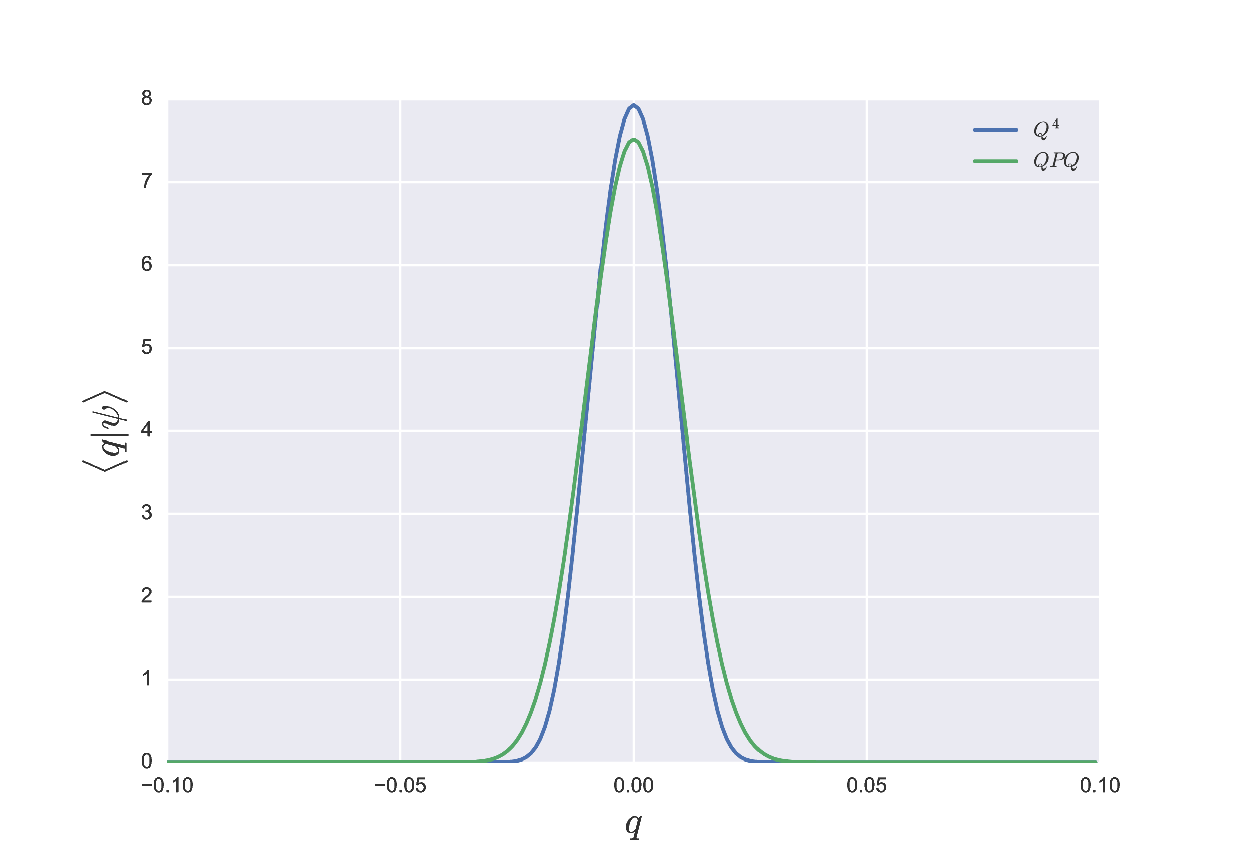
\includegraphics[width = 9cm]{./EPS/psi_qpq2.eps}
        \caption{固有関数の絶対値($H_z^v,\ H_z^v + 2BQPQ$)}\label{psi_qpq}
      \end{center}
    \end{minipage}
    \begin{minipage}{0.6\hsize}
      \begin{center}
        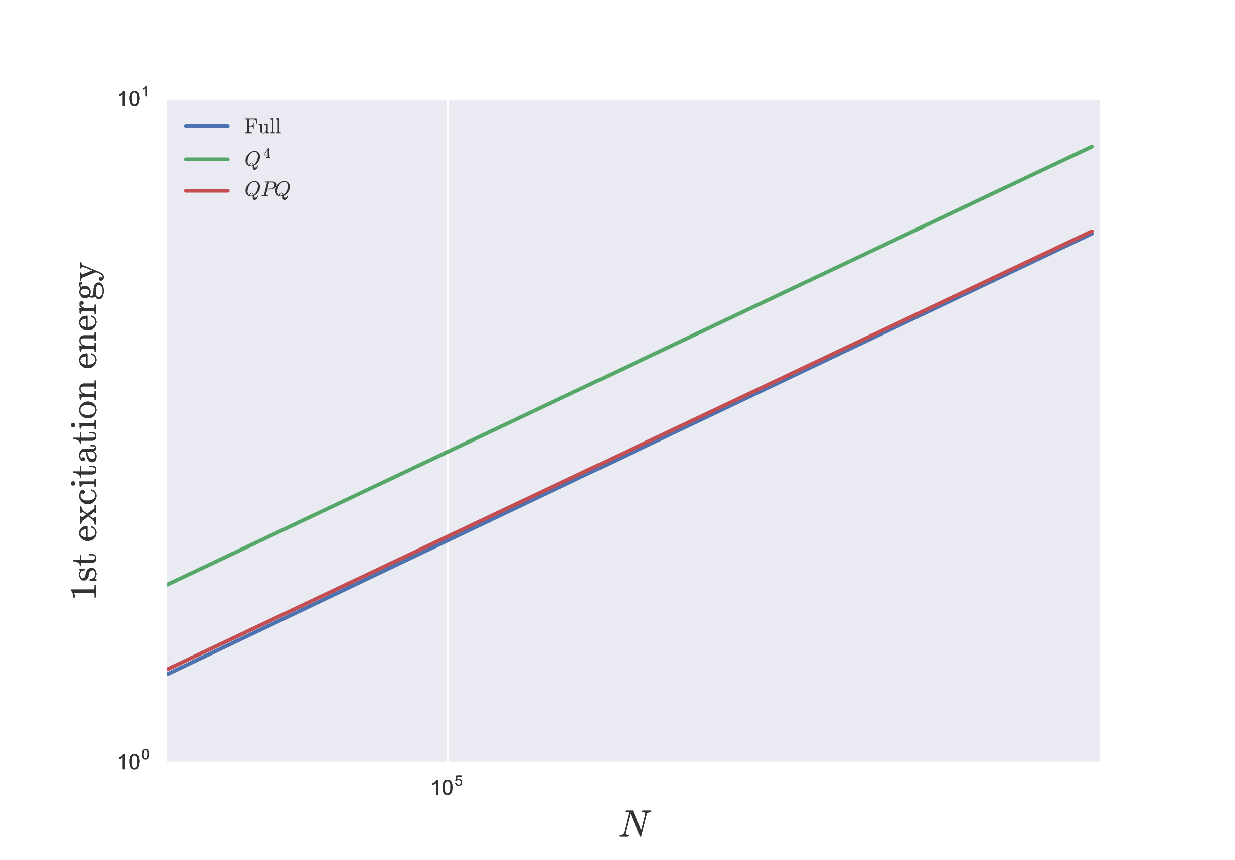
\includegraphics[width = 9cm]{./EPS/energy2.eps}
        \caption{エネルギー固有値($H_z,\ H_z^v,\ H_z^v + 2BQPQ$)}\label{energy}
      \end{center}
    \end{minipage}
  \end{tabular}
\end{figure}

\section{試行関数の類推}
試行関数が満たすべき条件は,
\begin{itemize}
\item[1.] \textbf{場の分割条件$\ev{Q}{\Psi} = \ev{P}{\Psi} = 0$}
\item[2.] \textbf{$|\bra{q}\ket{\Psi}|$は$q=0$にピークを持つ偶関数}
\item[3.] \textbf{$\ev{QPQ}{\Psi}\neq 0$}
\end{itemize}
であるように思われる. 1は対称性の自発的破れによるものであり, 2はゼロモードハミルトニアン$Q$の空間反転対称性から. 1, 3の条件を書き下すと
\begin{eqnarray}
  \int_{-\infty}^{\infty} dq\; q\Psi^*\Psi = 0 \hspace{0.3cm} and \hspace{0.3cm} -i\int_{-\infty}^{\infty} dq \Psi^*\frac{d}{dq}\Psi = 0 \hspace{0.3cm} and \hspace{0.3cm} -i\int_{-\infty}^{\infty} dq\; q^2 \Psi^*\frac{d}{dq}\Psi \neq 0
\end{eqnarray}
$\ev{Q}{\Psi} = 0$を満たす関数を選ぶことは難しくない\footnote{Taylor展開可能な関数ならOK?}. 一方で, $\ev{P}{\Psi} = 0$かつ$\ev{QPQ}{\Psi}\neq 0$は自明ではない. 条件2に倣って試行関数を偶関数に選ぶと, $\ev{QPQ}{\Psi} = 0$となってしまう. 仮に奇関数に選んだとしても同様である. つまり, 選ぶべきは偶関数でも奇関数でもないものになる. $\int_{-\infty}^{\infty} dq\; q^2 \Psi^*\frac{d}{dq}\Psi \neq 0$を満たすには$\int_{-\infty}^{\infty} dq \Psi^*\frac{d}{dq}\Psi = 0$ の根拠が「$\Psi^*\frac{d}{dq}\Psi$が奇関数」であってはならないことからもわかる. これは一見条件2に反しているように思えるが, 試行関数を複素数に拡張することで条件2を満たすことは可能である.
\subsection{固有関数の実部と虚部}
固有関数のイメージを膨らませるために固有関数をプロットする(図\ref{psi2_phase}).実部と虚部が偶関数でも奇関数でもない異様な構造を持っているが, 固有関数の位相の基準の取り方によっては実部と虚部は形を変え得るので, $q=0$の位相を基準に取り直してプロットしてみる(図 \ref{psi}). 
\begin{figure}[H]
  \begin{tabular}{cc}
    \begin{minipage}{0.5\hsize}
      \begin{center}
        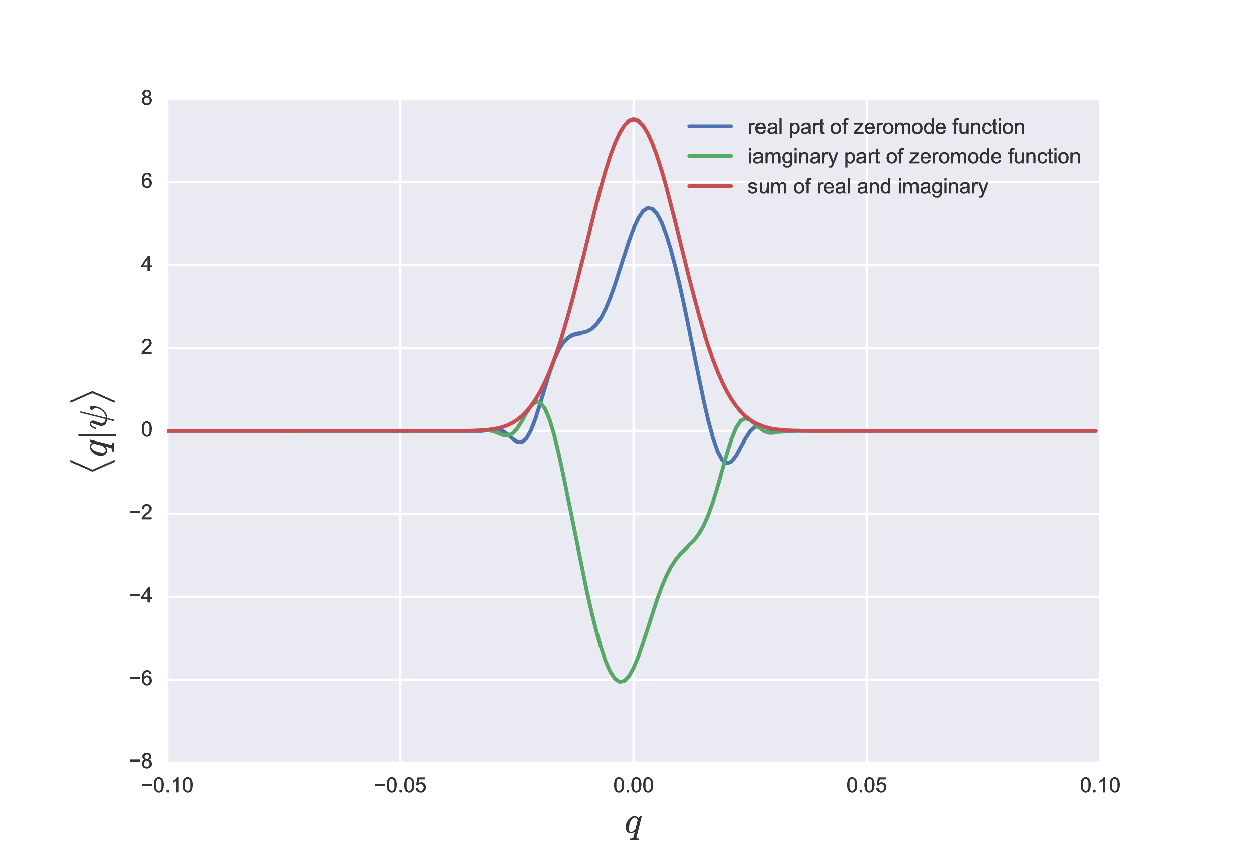
\includegraphics[width = 9cm]{./EPS/psi_phase2}
        \caption{固有関数の実部と虚部}\label{psi2_phase}
      \end{center}
    \end{minipage}
    \begin{minipage}{0.6\hsize}
      \begin{center}
        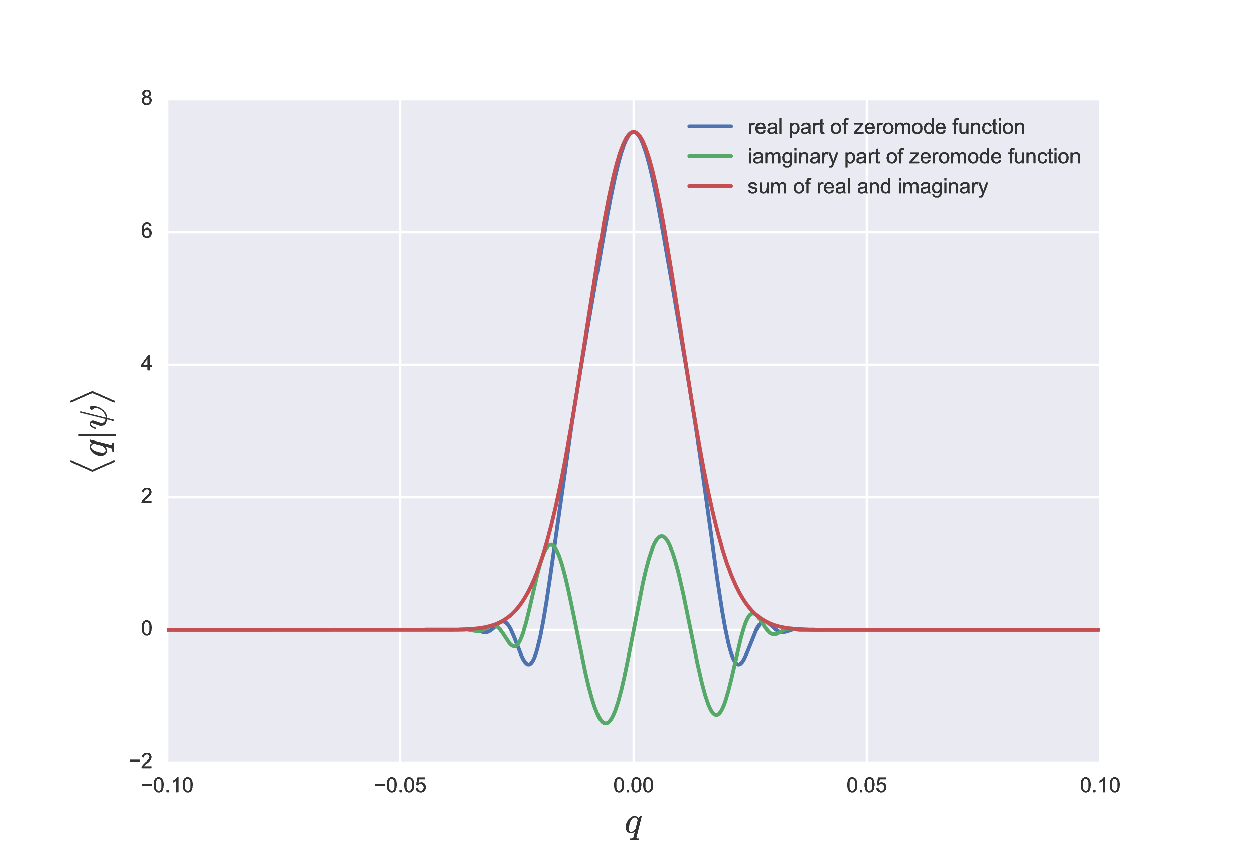
\includegraphics[width = 9cm]{./EPS/psi2}
        \caption{固有関数の実部と虚部(modified)}\label{psi}
      \end{center}
    \end{minipage}
  \end{tabular}
\end{figure}
\noindent これにより, 試行関数の満たすべき条件として 
\begin{itemize}
\item[4.] \textbf{$\Psi$の実部は偶関数, 虚部は奇関数}
\end{itemize}
が追加される. 
\subsubsection{試行関数の類推 - 仮定その1}
このグラフを見る限り試行関数は
\begin{eqnarray}
  \Psi &=& \qty(\frac{1}{2\pi\alpha^2})^\frac14e^{-\frac{q^2}{4\alpha^2} + i\beta q}\\
  \Re[\Psi] = \qty(\frac{1}{2\pi\alpha^2})^\frac14e^{-\frac{q^2}{4\alpha^2}}\cos(\beta q), &&\hspace{0.5cm}\Im[\Psi] = \qty(\frac{1}{2\pi\alpha^2})^\frac14e^{-\frac{q^2}{4\alpha^2}}\sin(\beta q)
\end{eqnarray}
が妥当であるように思える. これは$|\Psi|$がガウシアンになっていることから条件2を満たしている. \textbf{しかし図 \ref{psi}をよく見ると節の周期が一定になっていない上に, $\alpha, \beta$を動かしても$\ev{P}=0$を満たす構造を作ることは不可能である.} もう少し精査が必要である.
\subsection{期待値の実部と虚部}
ここで$\ev{P}$と$\ev{QPQ}$の被積分関数をプロットしてみる(図 \ref{P_2}-\ref{QPQ}).
\begin{figure}[H]
  \begin{tabular}{cc}
    \begin{minipage}{0.5\hsize}
      \begin{center}
        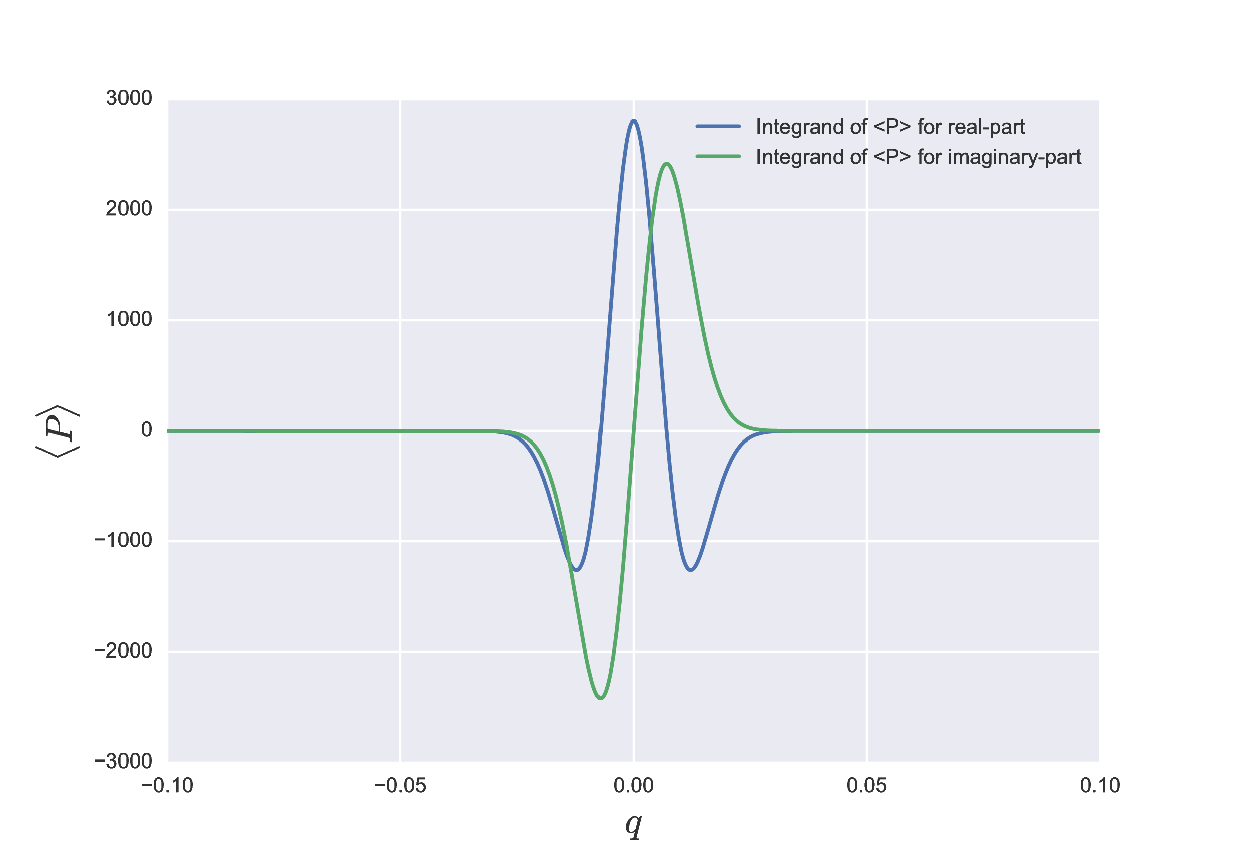
\includegraphics[width = 9cm]{./EPS/P_2.eps}
        \caption{$\ev{P}$の実部と虚部(被積分関数)}\label{P_2}
      \end{center}
    \end{minipage}
    \begin{minipage}{0.6\hsize}
      \begin{center}
        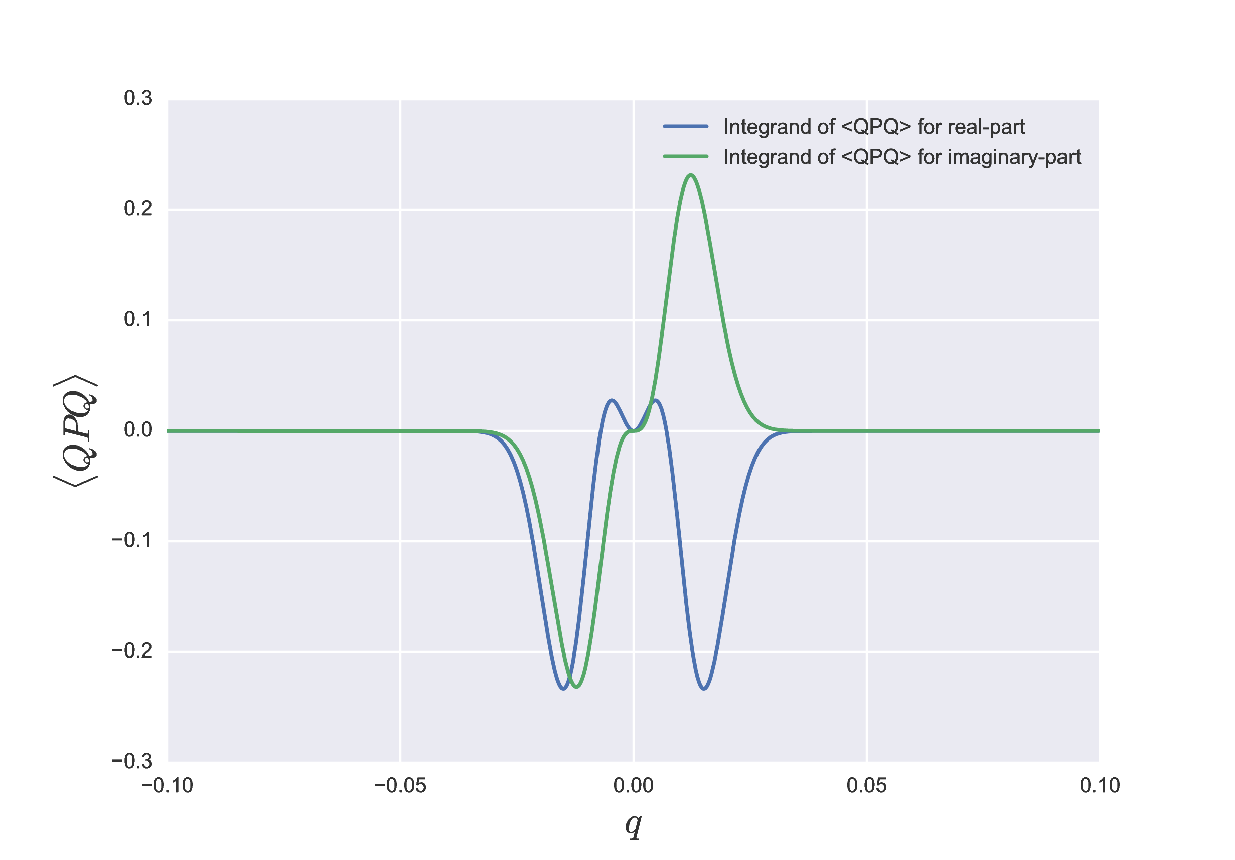
\includegraphics[width = 9cm]{./EPS/QPQ2.eps}
        \caption{$\ev{QPQ}$の実部と虚部(被積分関数)}\label{QPQ}
      \end{center}
    \end{minipage}
  \end{tabular}
\end{figure}
これは, 条件1・3を同時に満たす理由を被積分関数の実部が担っていることを示唆している. 被積分関数の虚部は固有関数の実部\footnote{正確には試行関数をGaussian-likeに取ったときの指数の肩の実部.}によるものであり, \textbf{試行関数の偶関数部がガウシアンであるなら$\ev{P}$および$\ev{QPQ}$の虚部は$qe^{-q^2}$のような奇関数になる.} これは上のグラフとほぼ同じ挙動を示しているだろう. やはり試行関数は$\qty(\frac{1}{2\pi\alpha^2})^\frac14e^{-\frac{x^2}{4\alpha^2}} \times e^{i\bullet}$とするのが妥当である. 一方で被積分関数の実部については虚部ほど自明ではない.
\subsubsection{試行関数の類推 - 仮定その2}
\begin{eqnarray}
  \Re[P] = \qty(\frac{1}{2\pi\alpha^2})^\frac14e^{-\frac{q^2}{4\alpha^2}}\cos(\beta q)
\end{eqnarray}
という仮定をしてみる. これはつまり試行関数が
\begin{eqnarray}
  \Psi &=& \qty(\frac{1}{2\pi\alpha^2})^\frac14e^{-\frac{q^2}{4\alpha^2} + i \sin(\beta q)}
\end{eqnarray}
であるということ. しかしこれは図 \ref{psi}における周期の問題を解決できておらず, かつ$\ev{P}=0$を満たすこともできない.

\subsubsection{試行関数の類推 - 仮定その3}
そもそも固有関数の振動周期が$q$-依存性を持つような構造はどのような試行関数によって得られるかというと, 例えば以下のようなものが挙げられる:
\begin{eqnarray}
  \Psi &=& \qty(\frac{1}{2\pi\alpha^2})^\frac14e^{-\frac{q^2}{4\alpha^2} + i\beta q^n}\\
  \Re[\Psi] = \qty(\frac{1}{2\pi\alpha^2})^\frac14e^{-\frac{q^2}{4\alpha^2}}\cos(\beta q^n), &&\hspace{0.5cm}\Im[\Psi] = \qty(\frac{1}{2\pi\alpha^2})^\frac14e^{-\frac{q^2}{4\alpha^2}}\sin(\beta q^n)
\end{eqnarray}
しかし, $n$が奇だと$\ev{P}\neq0$になる. さらに, どんな$n$であっても図 \ref{P_2}のような概形にはならない. 

様々な問題はあるものの, 周期の問題の解決はこの形式が最も単純であるように思える.

\subsubsection{試行関数の類推 - 仮定その4}
仮定その3の拡張した以下のような試行関数は, 上記の問題をすべて解決できる可能性を持っている:
\begin{eqnarray}
  \Psi &=& \qty(\frac{1}{2\pi\alpha^2})^\frac14e^{-\frac{q^2}{4\alpha^2} + i\sum_n \lambda_nq^{2n+1}} \label{trial-assumption}
\end{eqnarray}
しかしこれでは自由度(変分パラメータ)が大きすぎるため, どこかで和を打ち切る必要がある. そこで最も単純なものを採用する:
\begin{eqnarray}
  \Psi &=& \qty(\frac{1}{2\pi\alpha^2})^\frac14e^{-\frac{q^2}{4\alpha^2} + i(\beta q + \gamma q^3)}\label{trial}
\end{eqnarray}
\textbf{これは条件1-4をすべて満たすことができる.}
\subsection{変分パラメータ}
系の情報から変分パラメータを限定していく.
\subsubsection{条件1 : $\ev{P} = 0$}
条件2-4及び$\ev{Q} = 0$は関数の形によって既に満たされている. $\ev{P} = 0$を満たすとき, 変分パラメータに条件が課される:
\begin{eqnarray}
  &&\ev{P} = \qty(\frac{1}{2\pi\alpha^2})^\frac14\int dq \qty(\beta e^{-\frac{q^2}{2\alpha^2}} + 3\gamma q^2 e^{-\frac{q^2}{2\alpha^2}}) =0\\
  &&\therefore \beta + 3\gamma\alpha^2 = 0 \label{condition1}
\end{eqnarray}
\subsubsection{$\ev{P}$の特殊性}
条件1-4のもとでは変分パラメータは1つしか削ることができない. このまま変分近似に進むのはあまり得策ではないので, もう少し条件がないかを探すことにする.

実は$\ev{P}$の被積分関数について
\begin{eqnarray}
  RP &\equiv& \int dq \Re\qty[-i\int_{-\infty}^{\infty} dq \Psi^*\frac{d}{dq}\Psi]^2 = \frac{27}{8}\alpha^4\gamma^2\\
  IP &\equiv& \int dq \Re\qty[-i\int_{-\infty}^{\infty} dq \Psi^*\frac{d}{dq}\Psi]^2= \frac{1}{16\alpha^2}\\
  \frac{RP}{IP} &=& {\rm const}
\end{eqnarray}
という性質を持っている.\textbf{ constというのは可変パラメータである$g$にも$N$にも依存しないという意味.} これは図\ref{P_2}の実部と虚部の面積比が一定であることを示している. この$RP$と$IP$の比が具体的にどうなるかを決めるのは, (恐らく)(\ref{trial-assumption})における$\sum_n \lambda_nq^{2n+1}$がどのような関数のTaylor展開に対応しているかである. それを調べる手段はつまるところ数値計算結果と比較する他なく, $RP/IP$を具体的に求めてみることと同等である. \textbf{数値計算の結果, $RP/IP=3/4$になることがわかった\footnote{この結果から, 具体的な関数を予想できるかもしれない. 個人的にはシグモイド的な何かだと思っているが, $\ev{P}=0$を満たすような関数を見つけられない可能性も当然ある. フーリエ解析してみるのもいいかもしれない. }.} これにより
\begin{eqnarray}
  72\alpha^6\gamma^2 = 1\label{condition2}
\end{eqnarray}
という条件を得る. (\ref{trial})(\ref{condition1})(\ref{condition2})をまとめると
\begin{itembox}[c]{新しい試行関数}
\begin{eqnarray}
  &&\Psi = \qty(\frac{1}{2\pi\alpha^2})^\frac14e^{-\frac{q^2}{4\alpha^2} + i(\beta q + \gamma q^3)}\label{new-trial}\\
  &&\beta + 3\gamma\alpha^2 = 0,\hspace{1cm} 72\alpha^6\gamma^2 = 1 \label{conditions}\\
  &&\Rightarrow \beta = \pm\frac{1}{2\sqrt{2}\alpha}\hspace{1cm}\gamma = \mp\frac{1}{6\sqrt{2}\alpha^3}
\end{eqnarray}
\end{itembox}
これで変分近似の準備ができた.
\section{変分近似}
\subsection{$\alpha$のオーダー}
エネルギーの主要項が$P^2, Q^4, QPQ$であることを仮定して変分近似を進める\footnote{他の項が効いてこないことを確かめてみてほしい. }. 各期待値は以下の通り:
\begin{eqnarray}
  \ev{Q^4} = 3\alpha^4, \hspace{1cm}\ev{P^2} = \frac{1}{2\alpha^2}\hspace{1cm}\ev{QPQ} = \alpha^2 - \frac{3\alpha}{2\sqrt{2}}\simeq - \frac{3\alpha}{2\sqrt{2}}
\end{eqnarray}
$QPQ$はエネルギーを下げることから主要項右辺第二項である. これによりエネルギーは
\begin{eqnarray}
  f(\alpha) = \frac32A\alpha^4 + \frac{I}{4\alpha^2} - \frac{3}{\sqrt{2}}B\alpha
\end{eqnarray}
となる. ここでも$D$が主要項にならないことを見越して落としている. 微分すると
\begin{eqnarray}
  f'(\alpha) = 6A\alpha^3 - \frac{I}{2\alpha^3} - \frac{3}{\sqrt{2}}B
\end{eqnarray}
$f'(\alpha)=0$として一様系の$A, B, I$を代入すると
\begin{eqnarray}
  &&6N_0^2\alpha^6 - \frac{1}{2} - \frac{3}{2\sqrt{2}}N_0\alpha^3 = 0\\
  &&\therefore \alpha = \sqrt[3]{\frac{3 + \sqrt{105}}{24\sqrt{2}}}N_0^{-\frac13}\simeq 0.731N_0^{-\frac13}
\end{eqnarray}
$QPQ$を入れない変分法に比べて$\alpha$のオーダーは当然変化しないが, 従来の変分法だと$N_0^{-\frac13}$の係数が$0.588...$程度であったのに対して少し持ち上がった結果が得られた. このことから, \textbf{$QPQ$を入れるかどうかですべてのゼロモード期待値が影響を受ける}ということがわかる. 
\subsection{期待値の}
\newpage
\chapter{Fetter-Walecka : Quantum Theory of Many-Particle Systems(Dover, 1971)}
ちゃんと式まで書いて説明しているところもあれば, 原文の式番号だけ書いて済ませているところもあります. 原文の補助に過ぎないものだと思ってください. 
\section{Second Quantization}
だいたい知っていると思うので, Fetterの流儀を知るために簡単におさらいするに留める.
\subsection{Fields}
生成消滅演算子の線型結合について:
\begin{eqnarray}
  \hat{\psi}(\bm{x}) &\equiv& \sum_k\psi_k(\bm{x})c_k\label{2nd-quantum1}\\
  \hat{\psi}^\dagger(\bm{x}) &\equiv& \sum_k\psi_k^\dagger(\bm{x})c^\dagger_k\label{2nd-quantum2}
\end{eqnarray}
展開係数は一粒子波動関数で完全系による展開だと思えば良い\footnote{原書は ``complete set of single-particle quantum numbers'' とある. $\psi$がハミルトニアンの固有関数ならエネルギー固有関数による完全系であるし, 運動量演算子の固有関数なら運動量固有関数の完全系で展開ということになる. `` quantum numbers'' はここで言えばエネルギーか運動量か, みたいな話. }. ここで$\psi$はスピンについてのdoubletであり, $k$はなんかしらのquantum number\footnote{繰り返しになるが, 例えば主量子数・方位量子数・磁気量子数で$\bm{k} = (n, l, m)$みたいなのはよくあるよね. }:
\begin{eqnarray}
  \psi_k(\bm{x}) =
  \begin{pmatrix}
    \psi_{k1}(\bm{x})\\
    \psi_{k2}(\bm{x})
  \end{pmatrix}
  \equiv \psi_{k\alpha}(\bm{x}) & (\alpha = 1, 2)
\end{eqnarray}
$\alpha$はスピンのインデックス. $\hat{\psi}, \hat{\psi}^\dagger$は場の演算子と呼ばれる. 場の演算子は生成消滅演算子を含んでいるのでFock空間の演算子である. 場の演算子は正準交換関係を満たす:
\begin{eqnarray}
  \qty[\hat{\psi}_\alpha(\bm{x}), \hat{\psi}_\beta^\dagger(\bm{x}')]_{\mp} &=& \delta_{\alpha\beta}\delta(\bm{x} - \bm{x}')\\
  \qty[\hat{\psi}_\alpha(\bm{x}), \hat{\psi}_\beta(\bm{x}')]_{\mp} &=&\qty[\hat{\psi}^\dagger_\alpha(\bm{x}), \hat{\psi}^\dagger_\beta(\bm{x}')]_{\mp} = 0
\end{eqnarray}
$-$がボソン, $+$がフェルミオンである. 上の式はこれは生成消滅演算子の正準交換関係から得られ, 下の式は波動関数の完全性から得られる.

ハミルトニアンは場の演算子を用いて以下のように書き直せる:
\begin{eqnarray}
  \hat{H} = \int d\bm{x} \hat{\psi}^\dagger(\bm{x})T(\bm{x})\hat{\psi}(\bm{x}) + \frac{1}{2}\int\int d\bm{x}d\bm{x}' \hat{\psi}^\dagger(\bm{x})\hat{\psi}^\dagger(\bm{x}')V(\bm{x}, \bm{x}')\hat{\psi}(\bm{x}')\hat{\psi}(\bm{x})
\end{eqnarray}
$T(\bm(x))$はkinetic energy term. これがなぜハミルトニアンと呼んでよいかは山中先生の資料を参照のこと\footnote{(\ref{2nd-quantum1})(\ref{2nd-quantum2})をハミルトニアンの定義に代入すると多体量子力学のハミルトニアンが再現できる. }.

ここで一般的な一体演算子\footnote{Green関数・相関関数のような2体関数でないという意味}を考える:
\begin{eqnarray}
  J = \sum_{i = 0}^NJ(\bm{x_i})
\end{eqnarray}
なんかしらの演算子$J(\bm{x_i})$の線型結合として定義された第一量子化\footnote{第二量子化ではないというニュアンス. 第一量子化という言葉が的確かどうかは知らない. }された演算子. これを第二量子化の表示に移すと以下のようになる\footnote{(\ref{2nd-quantum3})は少々雑な議論っぽい. 運動量演算子を第二量子化したときのアナロジーが根拠か? いずれにしろ, 変換のgeneratorとして定義するほうが筋が通っているように思える. 第二量子化は場の理論よりも不完全である. }:
\begin{eqnarray}
  \hat{J} &=& \sum_{rs}\bra{r}J\ket{s}c_r^\dagger c_s\label{2nd-quantum3}\\
  &=& \int d\bm{x}\sum_{rs}\hat{\psi}^\dagger_r(\bm{x})J(\bm{x})\hat{\psi}_s(\bm{x})c_r^\dagger c_s\\
  &=& \int d\bm{x}\hat{\psi}^\dagger(\bm{x})J(\bm{x})\hat{\psi}(\bm{x})
\end{eqnarray}
以降Fetterの本では第二量子化の際はこの(\ref{2nd-quantum3})を使う. その是非はともかくとして. 

\section{Green's Functions}
このセクションではGreen関数\footnote{propagatorとかも呼ばれる}のコンセプトについて紹介する. Green関数は多体問題の取り扱いの上で重要な働きをする. 以下描像を明確にするために原書にはない添字$S, H$をつける. 
\subsection{Definition}
Green関数の定義は以下の通り:
\begin{eqnarray}
  iG_{\alpha\beta}(\bm{x}, t;\bm{x}', t') = \frac{\!_H\bra{\Psi_0}T\qty[\hat{\psi}_{H\alpha}(\bm{x}t)\hat{\psi}_{H\beta}^\dagger(\bm{x}'t')]\ket{\Psi_0}_H}{\!_H\bra{\Psi_0}\ket{\Psi_0}_H}\label{definition-green}
\end{eqnarray}
$\ket{\Psi_0}_H$は相互作用系のHeisenberg Full Hamiltonianの基底固有状態:
\begin{eqnarray}
  H_H\ket{\Psi_0}_H = E\ket{\Psi_0}_H 
\end{eqnarray}
$\hat{\psi}_{H\alpha}(\bm{x}t)$はHeisenberg描像の時間依存演算子:
\begin{eqnarray}
  \hat{\psi}_{H\alpha}(\bm{x}t) = e^{i\hat{H_H}t/\hbar}\hat{\psi}_{S\alpha}(\bm{x})e^{-i\hat{H_H}t/\hbar}
\end{eqnarray}
$\alpha\beta$は場の演算子の内部自由度であり, 今回はスピン1/2のフェルミオンを考える. T積の部分を書き下すと
\begin{eqnarray}
  T\qty[\hat{\psi}_{H\alpha}(\bm{x}t)\hat{\psi}_{H\beta}^\dagger(\bm{x}'t')] =
  \begin{cases}
    \hat{\psi}_{H\alpha}(\bm{x}t)\hat{\psi}_{H\beta}^\dagger(\bm{x}'t') & (t > t')\\
    \pm\hat{\psi}_{H\beta}^\dagger(\bm{x}'t')\hat{\psi}_{H\alpha}(\bm{x}t) & (t < t')
  \end{cases}
\end{eqnarray}
ここで符号が$+$ならボソン, $-$ならフェルミオン. つまるところ, T積は時間順序通りに演算子を並べ替えて, 演算子を入れ替えた回数を$P$とするとき, 先頭に$(-1)^P$を付ければ良い\footnote{もちろんフェルミオンの場合. ボソンの場合は$(-1)^P$因子はいらない}. というわけで, (\ref{definition-green})をexplicitに書き直すと
\begin{eqnarray}
  iG_{\alpha\beta}(\bm{x}, t;\bm{x}', t') =
  \begin{cases}
    \cfrac{\!_H\bra{\Psi_0}\hat{\psi}_{H\alpha}(\bm{x}t)\hat{\psi}_{H\beta}^\dagger(\bm{x}'t')\ket{\Psi_0}_H}{\!_H\bra{\Psi_0}\ket{\Psi_0}_H} & (t > t')\\
    \pm\cfrac{\!_H\bra{\Psi_0}\hat{\psi}_{H\beta}^\dagger(\bm{x}'t')\hat{\psi}_{H\alpha}(\bm{x}t)\ket{\Psi_0}_H}{\!_H\bra{\Psi_0}\ket{\Psi_0}_H} & (t < t')
  \end{cases}
  \label{definition-green2}
\end{eqnarray}
Green関数というのは$(\bm{x}, t), (\bm{x}', t)$にある場の演算子の期待値である\footnote{だから2点関数とか2点相関関数とかも呼ばれる}. $\ket{\Psi_0}_H$がHeisenberg Full Hamiltonianであることから演算子をSchr\"odinger描像に書き換えると
\begin{eqnarray}
  iG_{\alpha\beta}(\bm{x}, t;\bm{x}', t') =
  \begin{cases}
    e^{iE(t-t')/\hbar}\cfrac{\!_H\bra{\Psi_0}\hat{\psi}_{S\alpha}(\bm{x})e^{-i\hat{H}_H(t-t')}\hat{\psi}_{S\beta}^\dagger(\bm{x}')\ket{\Psi_0}_H}{\!_H\bra{\Psi_0}\ket{\Psi_0}_H} & (t > t')\\
    \pm e^{-iE(t-t')/\hbar}\cfrac{\!_H\bra{\Psi_0}\hat{\psi}_{S\beta}^\dagger(\bm{x}')e^{i\hat{H}_H(t-t')}\hat{\psi}_{S\alpha}(\bm{x})\ket{\Psi_0}_H}{\!_H\bra{\Psi_0}\ket{\Psi_0}_H} & (t < t')
  \end{cases}
  \label{definition-green3}
\end{eqnarray}
\subsection{Relation to Observables}
Green関数を勉強する理由はいくらかあって, そのひとつはFeynman diagramである. Feynman ruleで摂動計算をするときに場の演算子の積よりもGreen関数で表現するほうがシンプルになる. また, (\ref{definition-green})は基底固有関数で期待値を取っているため基底状態の情報がいくらか失われているのだが, 依然として興味深いオブザーバブルの特徴を保有している:
\begin{itemize}
\item 基底状態における様々な一粒子演算子の期待値
\item 基底エネルギー
\item スペクトラム
\end{itemize}
3つ目はLehmann表示で扱う\footnote{山中先生によれば, もともとは梅沢・亀淵・Lehmann表示と呼ばれていたらしい. 最近は普通にスペクトラム表示とか言う. }. 以下では上2つについて説明する.

まず一粒子演算子を考える:
\begin{eqnarray}
  \hat{J}_S &=& \int d\bm{x} {\cal \hat{J}}_S(\bm{x})\\
  \hat{{\cal J}}_S(\bm{x}) &=& \sum_{\alpha\beta}\hat{\psi}_{\beta S}^\dagger(\bm{x})J_{\beta\alpha}(\bm{x})\hat{\psi}_{\alpha S}(\bm{x})
\end{eqnarray}
$\hat{J}$は第二量子化された演算子. $J_{\beta\alpha}$は密度に関する第一量子化演算子であり$\hat{{\cal J}}$はそれを第二量子化したもの. $\ev{\hat{\cal{J}}(\bm{x})}$について:
\begin{eqnarray}
  \ev{\hat{\cal J}(\bm{x})} &=& \frac{\!_H\bra{\Psi_0}\hat{\cal J}(\bm{x})\ket{\Psi_0}_H}{\!_H\bra{\Psi_0}\ket{\Psi_0}_H} \\
  &=& \lim_{\bm{x}'\rightarrow\bm{x}}\sum_{\alpha\beta}J_{\beta\alpha}\frac{\!_H\bra{\Psi_0}\hat{\psi}^\dagger_{\beta S}(\bm{x}')\hat{\psi}_{\alpha S}(\bm{x})\ket{\Psi_0}_H}{\!_H\bra{\Psi_0}\ket{\Psi_0}_H} \\
  &=& \lim_{t'\rightarrow t^+}\lim_{\bm{x}'\rightarrow\bm{x}}\sum_{\alpha\beta}J_{\beta\alpha}\frac{\!_H\bra{\Psi_0}\hat{\psi}^\dagger_{\beta S}(\bm{x}')e^{-i\hat{H}_H(t-t')/\hbar}\hat{\psi}_{\alpha S}(\bm{x})\ket{\Psi_0}_H}{\!_H\bra{\Psi_0}\ket{\Psi_0}_H} \\
  &=& \pm i\lim_{t'\rightarrow t^+}\lim_{\bm{x}'\rightarrow\bm{x}}\sum_{\alpha\beta}J_{\beta\alpha}G_{\alpha\beta}(\bm{x}, t; \bm{x}', t')\label{before-trace}\\
  &=& \pm i\lim_{t'\rightarrow t^+}\lim_{\bm{x}'\rightarrow\bm{x}}\Tr\qty[J(\bm{x})G(\bm{x}, t; \bm{x}', t')]
\end{eqnarray}
2行目で$\bm{x}'$を登場させたり, 3行目に$\hat{1} = \lim_{t'\rightarrow t^+}e^{-iH_H(t - t')/\hbar}$を持ってきたりしたのは全てGreen関数に帰着させるためのテクニック. $G, J$は
\begin{eqnarray}
  G(\bm{x}) =
  \begin{pmatrix}
    G_{\uparrow\uparrow} & G_{\uparrow\downarrow}\\
    G_{\downarrow\uparrow} & G_{\downarrow\downarrow}
  \end{pmatrix} &  J(\bm{x}) =
  \begin{pmatrix}
    J_{\uparrow\uparrow} & J_{\uparrow\downarrow}\\
    J_{\downarrow\uparrow} & J_{\downarrow\downarrow}
  \end{pmatrix}
\end{eqnarray}
みたいな二階テンソル. これの積のトレースを取ると(\ref{before-trace})みたいになる. これが$J_{\alpha\beta}$ではなく$J_{\beta\alpha}$という表式にした理由.

例えば運動エネルギーの第一量子化は
\begin{eqnarray}
  P = -\frac{\hbar^2}{2m}\nabla^2
\end{eqnarray}
であり, これを第二量子化する:
\begin{eqnarray}
  \hat{P} &=& \int d\bm{x} \hat{{\cal P}}(\bm{x})\\
  \hat{{\cal P}}(\bm{x}) &=& \sum_{\alpha\beta}\hat{\psi}^\dagger_\beta(\bm{x})P_{\beta\alpha}\hat{\psi}_\alpha(\bm{x})\\
  \ev{P} &=& \pm i\int d\bm{x}'\lim_{\bm{x}' \rightarrow \bm{x}}\qty[-\frac{\hbar^2\nabla^2}{2m}\Tr G(\bm{x}t, \bm{x}'t^+)]
\end{eqnarray}
...工事中...
\subsection{Example : Free Fermion}
\subsection{Lehmann Representation}
この章ではフェルミオンについてのみ議論する. 状態が規格化されているものとするとGreen関数の定義は
\begin{eqnarray}
  iG_{\alpha\beta}(\bx t;\bx' t') = \!_H\bra{\Psi_0}T\qty[\psi_{H\alpha}(\bx t)\psi_{H\beta}^\dagger(\bx't)]\ket{\Psi_0}_H
\end{eqnarray}
Heisenberg描像の演算子と状態はかなり複雑だが, 面白くかつ一般的な結果を導くことができる. まず$\qty{\ket{\Psi}}$完全系を挿入:
\begin{eqnarray}
  \nonumber  iG_{\alpha\beta}(\bx t;\bx' t') = \sum_n\Big\{\theta(t-t')\bra{\Psi_0}\hat{\psi}_{\alpha H}(\bx t)\ket{\Psi_n}\bra{\Psi_n}\hat{\psi}^\dagger_{\beta H}(\bx't')\ket{\Psi_0}\\
  -\theta(t'-t)\bra{\Psi_0}\hat{\psi}^\dagger_{\beta H}(\bx' t')\ket{\Psi_n}\bra{\Psi_n}\hat{\psi}_{\alpha H}(\bx t)\ket{\Psi_0}\Big\}
\end{eqnarray}
さらにSchr\"odinger描像とHeisenberg描像の変換
\begin{eqnarray}
  \hat{O}_H(t) = e^{iH_Ht/\hbar}\hat{O}_Se^{-iH_Ht/\hbar}
\end{eqnarray}
を用いて場の演算子を変換するとエネルギー固有値がくくり出せる:
\begin{eqnarray}
  \nonumber    iG_{\alpha\beta}(\bx t;\bx' t') = \sum_n\Big\{\theta(t-t')e^{-i(E_n-E)(t-t')/\hbar}\bra{\Psi_0}\hat{\psi}_{\alpha S}(\bx)\ket{\Psi_n}\bra{\Psi_n}\hat{\psi}^\dagger_{\beta S}(\bx')\ket{\Psi_0}\\
  -\theta(t'-t)e^{i(E_n-E)(t-t')/\hbar}\bra{\Psi_0}\hat{\psi}^\dagger_{\beta S}(\bx')\ket{\Psi_n}\bra{\Psi_n}\hat{\psi}_{\alpha S}(\bx)\ket{\Psi_0}\Big\}
\end{eqnarray}
ここで, $\bra{\Psi_n}\hpsi\ket{\Psi_0}$について少し考えてみる. もし$\ket{\Psi_0}$が$N$個の粒子を含んでいる状態ならば, $\hpsi\ket{\Psi_0}$は$N-1$個の粒子を含む状態になるので, $\bra{\Psi_n}\hpsi\ket{\Psi_0}$が値を持つためには$\bra{\Psi_n}$が$N-1$個の粒子を含む状態でなければならない. 同様の議論から$\bra{\Psi_n}\hpsi^\dagger\ket{\Psi_0}$が値を持つためには$\ket{\Psi_n}$は$N+1$個の粒子を含む状態でなければならない. よって, $\ket{\Psi_n}$は$N\pm1$個の粒子を持つ状態である\footnote{この議論だと, 第一励起状態$\ket{\Psi_1}$, 第二励起状態$\ket{\Psi_2}$, 第三励起状態$\ket{\Psi_3}$...は全て$N\pm1$個の粒子を持つことになる. 基底だけ$N$個で残りの励起状態は全て$N\pm1$というのは少し不自然に感じる. いくらか理由を考える余地はあるが, まだ納得できる答えを持っていません. 少なくともそういう状況でなければGreen関数は値を持つことができない. }. さらに言うと, これは$\ket{\Psi_n}$が粒子数固有状態でなければならないので, BEC系のような粒子数が揺らぐ系では議論が破綻することに注意. これが, 今回Fermion系のみを考える理由である. 

ここまでの話は$\hat{H}_H$が時間非依存であるということ(と$\ket{\Psi}$が粒子数固有状態であること)を除けば一般的な議論である. このまま議論をすすめることもできるが, ここでは簡単のため運動量演算子が$\hat{H}_H$と交換する場合を考える\footnote{運動量演算子$\hat{P}$がHeisenberg Full Hamiltonian$\hat{H}_H$と交換するとき, $\hat{H}_H$の固有状態$\ket{\Psi_n}$は$\hat{P}$と同時固有状態を取るということである.}. まずは運動量演算子を並進変換のgeneratorとして導入する:
\begin{eqnarray}
  &&\hpsi_\alpha(\bx) \equiv e^{-i\hat{\bm{P}}x}\hpsi_\alpha(0)e^{i\hat{\bm{P}}x}\label{generator}\\
  \Longrightarrow&& -i\hbar\nabla\hpsi_\alpha(\bx) = \qty[\hpsi_\alpha(\bx), \hat{\bm{P}}]\\
  \Longrightarrow&& \hat{\bm{P}} = \sum_\alpha\int d\bx \hpsi^\dagger_\alpha(\bx)(-i\hbar\nabla)\hpsi_\alpha(\bx) = \sum_{\bm{k}\lambda}\hbar\bm{k}c^\dagger_{\bm{k}\lambda}c_{\bm{k}\lambda}
\end{eqnarray}
1行目を微分すると2行目になり, 2行目を満たすような$\hat{\bm{P}}$を探すと3行目になる. 3行目の2つ目のイコールは一粒子波動関数を
\begin{eqnarray}
  &&\psi_{\bm{k}\lambda}(\bx) = \frac{e^{i\bm{k}\bx}}{\sqrt{V}}\eta_{\lambda}\label{1st-plane}\\
  &&\eta_\uparrow =
  \begin{pmatrix}
    1\\
    0
  \end{pmatrix} \ \ \eta_\downarrow =
  \begin{pmatrix}
    0\\
    1
  \end{pmatrix}
\end{eqnarray}
のように平面波展開\footnote{Fourier変換のこと. 一様系だと並進対称性があり, 運動量が保存されるはず. だからハミルトニアンと運動量演算子は交換した. 先の通りハミルトニアンの固有状態は運動量固有状態にもなるので, Fourier変換してあげると運動量(c-数)が出てくる. 平面波展開はいつでもできるが, 状態がいつも運動量固有状態になっている訳はないことに注意. }して, これを式(\ref{2nd-quantum1})とかで第二量子化すれば得られる. $V$は体積. さて, この(\ref{generator})を先ほどのGreen関数の式に代入する:
\begin{eqnarray}
  \nonumber    iG_{\alpha\beta}(\bx t;\bx' t') = \sum_n\Big\{\theta(t-t')e^{-i(E_n-E)(t-t')/\hbar}e^{i\bm{P}_n\cdot(\bx - \bx')/\hbar}\bra{\Psi_0}\hat{\psi}_{\alpha S}(0)\ket{\Psi_n}\bra{\Psi_n}\hat{\psi}^\dagger_{\beta S}(0)\ket{\Psi_0}\\
  -\theta(t'-t)e^{i(E_n-E)(t-t')/\hbar}e^{-i\bm{P}_n\cdot(\bx - \bx')/\hbar}\bra{\Psi_0}\hat{\psi}^\dagger_{\beta S}(0)\ket{\Psi_n}\bra{\Psi_n}\hat{\psi}_{\alpha S}(0)\ket{\Psi_0}\Big\}
\end{eqnarray}
ここで基底状態では$\hat{\bm{P}}\ket{\Psi_0} = 0$となっていることを用いている. ここで, $G$は$\bx-\bx'$や$t-t'$にしか依存していないので$\bx-\bx' = \by$, $t-t' = s$としてFourier変換する:
\begin{eqnarray}
  G_{\alpha\beta}(\bk, \omega) &=& \int d\by\int ds\ e^{-i\bk\cdot\by}e^{i\omega s}G_{\alpha\beta}(\bx t; \bx't' )\\
  \nonumber  &=& -i\int d\by ds e^{-i\bm{k}\cdot\by}e^{i\omega s}\\
  \nonumber  &\times&\sum_n\Big[\ul{\theta(s)e^{-i(E_n- E)s/\hbar}e^{i\bm{P}_n\by/\hbar}\bra{\Psi_0}\hat{\psi}_{\alpha S}(0)\ket{\Psi_n}\bra{\Psi_n}\hat{\psi}^\dagger_{\beta S}(0)\ket{\Psi_0}}_{1}\\
    &&\ - \ul{\theta(-s)e^{i(E_n- E)s/\hbar}e^{-i\bm{P}_n\by/\hbar}\bra{\Psi_0}\hat{\psi}^\dagger_{\beta S}(0)\ket{\Psi_n}\bra{\Psi_n}\hat{\psi}_{\alpha S}(0)\ket{\Psi_0}}_2\Big]
\end{eqnarray}
ここで下線部1の項について計算する. $\theta$関数の積分表示
\begin{eqnarray}
  \theta(s) = -\int \frac{d\omega'}{2\pi i}\frac{e^{-i\omega' s}}{\omega' + i\eta}
\end{eqnarray}
を用いて変形していく:
\begin{eqnarray}
  \ul{ }1 &=& \frac{1}{2\pi}\sum_n\int d\by ds d\omega' e^{i(\bm{P}_n\hbar^{-1} - \bm{k})\cdot\by}e^{i(\omega - \qty(E_n - E)\hbar^{-1} -\omega')s}\frac{\bra{\Psi_0}\hat{\psi}_{\alpha S}(0)\ket{\Psi_n}\bra{\Psi_n}\hat{\psi}^\dagger_{\beta S}(0)\ket{\Psi_0}}{\omega' + i\eta}\\
  &=& \sum_n(2\pi)^3\delta(\bm{P}_n\hbar^{-1} - \bm{k})\frac{\bra{\Psi_0}\hat{\psi}_{\alpha S}(0)\ket{\Psi_n}\bra{\Psi_n}\hat{\psi}^\dagger_{\beta S}(0)\ket{\Psi_0}}{\omega - \qty(E_n - E)\hbar^{-1} + i\eta}\\
  &=& V\sum_n\delta_{\bm{P}_n\hbar^{-1},\bm{k}}\frac{\bra{\Psi_0}\hat{\psi}_{\alpha S}(0)\ket{\Psi_n}\bra{\Psi_n}\hat{\psi}^\dagger_{\beta S}(0)\ket{\Psi_0}}{\omega - \qty(E_n - E)\hbar^{-1} + i\eta}
\end{eqnarray}
最後の行でデルタ関数と体積の関係(\ref{delta-volume})を用いた. 同様の計算をすると, グリーン関数は
\begin{eqnarray}
  G_{\alpha\beta}(\bk, \omega) &=& V\sum_n\delta_{\bm{P}_n\hbar^{-1},\bm{k}}\frac{\bra{\Psi_0}\hat{\psi}_{\alpha S}(0)\ket{\Psi_n}\bra{\Psi_n}\hat{\psi}^\dagger_{\beta S}(0)\ket{\Psi_0}}{\omega - \qty(E_n - E)\hbar^{-1} + i\eta}\\ &+& V\sum_n\delta_{\bm{P}_n\hbar^{-1},-\bm{k}}\frac{\bra{\Psi_0}\hat{\psi}^\dagger_{\beta S}(0)\ket{\Psi_n}\bra{\Psi_n}\hat{\psi}_{\alpha S}(0)\ket{\Psi_0}}{\omega + \qty(E_n - E)\hbar^{-1} - i\eta}
\end{eqnarray}
となることがわかる. クロネッカーデルタが効いてくるのは$\ket{\Psi_n}$に対してなので
\begin{eqnarray}
  G_{\alpha\beta}(\bk, \omega) = V\sum_n\Big[\frac{\bra{\Psi_0}\hat{\psi}_{\alpha S}(0)\ket{n\bk}\bra{n\bk}\hat{\psi}^\dagger_{\beta S}(0)\ket{\Psi_0}}{\omega - \qty(E_n - E)\hbar^{-1} + i\eta}+ \frac{\bra{\Psi_0}\hat{\psi}^\dagger_{\beta S}(0)\ket{n, -\bk}\bra{n, -\bk}\hat{\psi}_{\alpha S}(0)\ket{\Psi_0}}{\omega + \qty(E_n - E)\hbar^{-1} - i\eta}\Big]
\end{eqnarray}
と書くことにする\footnote{ある$\bm{P}_n$に対応する$\bk$はひとつで, クロネッカーデルタなんか和を取って消えてしまうのでは?と思うかもしれない. しかし$\bk$はいくつもの準粒子のエネルギーの総和なので, $\bk$の選び方に対して同じエネルギーを持つものはいくつか存在する(縮退している?). 対して$\bm{P}_n$は$\hat{H}_H$の固有状態なので, $\ket{\Psi_n}$の縮退がなければ$\hat{P}_n$の縮退もない. そういうことで$\ket{\Psi_n}$を$n$と$\bk$でパラメトライズしている. これは一様系であるために運動量が保存し, そのquantum numberであるkを明示したに過ぎないらしい. そもそも$n$は様々なquantum numberを持っているが, 今回は$k$が保存するのでそれを外に出して$n$の定義を変えた, ということらしい. }. というわけで, これでGreen関数の周波数($\omega$)依存性を示すことができた. この分母についてもうちょっと詳細に見てみよう. 上式の第一項の分母は以下のように変形できる:
\begin{eqnarray}
  \omega - \hbar^{-1}\qty[E_n(N+1) - E(N)] = \omega - \hbar^{-1}\qty[E_n(N+1) - E(N+1)] -\hbar^{-1}\qty[E(N+1) - E(N)]
\end{eqnarray}
ここで$E(N+1) - E(N)$は基底状態に粒子が1つ追加された時のエネルギー差である. 粒子数変化に伴うエネルギー変化率をケミカルポテンシャルと呼ぶ. $E_n(N+1) - E(N+1)$は$N+1$粒子系の励起エネルギーである. そんなわけで, 書き直す:
\begin{eqnarray}
  G_{\alpha\beta}(\bk, \omega) = \hbar V\sum_n\Big[\frac{\bra{\Psi_0}\hat{\psi}_{\alpha S}(0)\ket{n\bk}\bra{n\bk}\hat{\psi}^\dagger_{\beta S}(0)\ket{\Psi_0}}{\hbar\omega -\mu - \epsilon_{n\bk}\qty(N+1) + i\eta}+ \frac{\bra{\Psi_0}\hat{\psi}^\dagger_{\beta S}(0)\ket{n, -\bk}\bra{n, -\bk}\hat{\psi}_{\alpha S}(0)\ket{\Psi_0}}{\hbar\omega -\mu + \epsilon_{n,-\bk}\qty(N-1) - i\eta}\Big]\label{green-rehmann}
\end{eqnarray}
$\eta$ に$\hbar^{-1}$がついていないが, $\eta$の定義の中に押し込めている. $\mu$も$N$依存性を持っているが
\begin{eqnarray}
  \mu(N+1) = \mu\qty(N\qty(1+\frac{1}{N})) = \mu(N) + O(N^{-1})
\end{eqnarray}
になるので, $N$が十分大きいものとして無視することにする.

これでスピン$\frac{1}{2}$の場合の$G$の行列構造についてシンプルにまとめることができた. このGreen関数は$2\times2$行列なので単位行列とPauli行列で構成される完全系で展開することができる\footnote{単に, 単位行列とパウリ行列の線型結合で書けるということ.}. 今回の問題は一様系なので指向性は無いため, $G$は空間回転に対してスカラー\footnote{ここでいうスカラーは"スカラー演算子"の意味. $\nabla = \qty(\partial_x, \partial_y, \partial_z)$はベクトル演算子, $\nabla\cdot\bk$はスカラー演算子. Pauli行列完全系も$\bm{\sigma} = \qty(\hat{\sigma}_x, \hat{\sigma}_y, \hat{\sigma}_z)$みたいなベクトル演算子だと考えれば$\bm{\sigma}\cdot\bk$もスカラー演算子である. }でなければならない. $G$には$\bm{\sigma}$と$\bk$が含まれるはずであり, $\bk$は$\bm{\sigma}$とペアになっていなければならないので
\begin{eqnarray}
  G(\bk, \omega) = a\bm{I} + b\bm{\sigma}\cdot\bk
\end{eqnarray}
という形になる. ここでハミルトニアンは空間鏡映対称性を持っており, この性質はGreen関数にも引き継がれているが, $\bm{\sigma}\cdot\bk$は擬スカラーなので鏡映対称性を持っていない. よって$b$の項は消えなければならない. これでGreen関数がとてもシンプルに書けることがわかる. (\ref{2nd-quantum1})(\ref{1st-plane})から場の演算子を平面波展開した表式
\begin{eqnarray}
  \hpsi(0) = \sum_k\frac{1}{\sqrt{V}}c_k
\end{eqnarray}
や
\begin{eqnarray}
  \epsilon_{\bk}(N+1) &=& \epsilon_{\bk}^0 - \epsilon_F^0 = \frac{\hbar^2(k^2 - k_F^2)}{2m}\\
  \mu &=& \epsilon_F^0
\end{eqnarray}
を用いるとFree FermionのGreen関数を再現できる:
\begin{eqnarray}
  G(\bk, \omega) = \delta_{\alpha\beta}\qty[\frac{\theta(k-k_F)}{\omega - \omega_k + i\eta} + \frac{\theta(k_F-k)}{\omega - \omega_k - i\eta}]
\end{eqnarray}
さて, ここで(\ref{green-rehmann})は$\hbar\omega$についての極を持つ関数である. $\epsilon_{n\bk}$が正定値なので$\Re\hbar\omega < \mu$ならば(\ref{green-rehmann})の第一項は極を持たない. 一方で$\Re\hbar\omega > \mu$ならば(\ref{green-rehmann})の第二項は極を持たない. これは原書のFig.7.1\footnote{$\hbar\omega$が複素数であることに注意. つまり, 縦軸が$\hbar\omega$の虚部, 横軸が実部.}のとおり. バッテンがGreen関数が極を持つ点を表している. 実軸よりちょっと上にあるか下にあるかは$i\eta$の符号が決めている. さて, Fig7.1を見てわかる通り, $\hbar\omega$の複素空間上では上部も下部も正則ではない. しかし, 今後の計算の上ではどちらか一方は正則であってほしい. ということで, 遅延Green関数・先進Green関数を定義する:
\begin{eqnarray}
  iG^R_{\alpha\beta}(\bx t;\bx't') &=& \bra{\Psi_0}\qty{\hpsi^\dagger_{H\alpha}(\bx t), \hpsi_{H\beta}(\bx't')}\ket{\Psi_0}\theta(t-t')\\
  iG^A_{\alpha\beta}(\bx t;\bx't') &=& \bra{\Psi_0}\qty{\hpsi_{H\beta}(\bx't'), \hpsi^\dagger_{H\alpha}(\bx t)}\ket{\Psi_0}\theta(t'-t)
\end{eqnarray}
これらは今までのGreen関数\footnote{因果Green関数という.}と同じように解析を進めることができ, 一様系でRehmann表示をしてみると
\begin{eqnarray}
  G_{\alpha\beta}^{R, A}(\bk, \omega) = \hbar V\sum_n\Big[\frac{\bra{\Psi_0}\hat{\psi}_{\alpha S}(0)\ket{n\bk}\bra{n\bk}\hat{\psi}^\dagger_{\beta S}(0)\ket{\Psi_0}}{\hbar\omega -\mu - \epsilon_{n\bk}\qty(N+1) \pm i\eta}+ \frac{\bra{\Psi_0}\hat{\psi}^\dagger_{\beta S}(0)\ket{n, -\bk}\bra{n, -\bk}\hat{\psi}_{\alpha S}(0)\ket{\Psi_0}}{\hbar\omega -\mu + \epsilon_{n,-\bk}\qty(N-1) \pm i\eta}\Big]\label{green-rehmann2}
\end{eqnarray}
となっている. 遅延Green関数の極は下部にまとまり, $\Im \omega > 0$の領域では解析的である. 先進はその逆. もし$\omega$が実なら
\begin{eqnarray}
  \qty[G_{\alpha\beta}^{R}(\bk, \omega)]^* = G_{\alpha\beta}^{A}(\bk, \omega)
\end{eqnarray}
の関係にある. 遅延と先進の違いは収束因子$i\eta$の符号のみである. もし$\omega$が実で$\hbar^{-1}\mu$より大きければ, 無限小の$i\eta$は何の役割も成さなくなる. 以上より
\begin{eqnarray}
  G_{\alpha\beta}^R(\bk, \omega) = G_{\alpha\beta}(\bk, \omega) & \Re\hbar\omega > \mu\\
  G_{\alpha\beta}^A(\bk, \omega) = G_{\alpha\beta}(\bk, \omega) & \Re\hbar\omega < \mu
\end{eqnarray}
\subsection{Physical Interpretation of the Green's Function}
一粒子Green関数の物理的な解釈を理解するために相互作用描像の状態$\ket{\Psi_I(t')}$と, $(\bx't')$に粒子を加える操作$\hpsi_{i\beta}(\bx't')\ket{\Psi_I(t')}$について考える. $\ket{\Psi_I(t')}$はハミルトニアンの固有状態ではないが, 時間発展演算子$\hat{U}(t, t')$は有効である. さて, $t>t'$において$\hat{U}(t, t')\hpsi_{I\beta}^\dagger(\bx't')\ket{\Psi_I(t')}$と$\hpsi^\dagger_{\bx t}\ket{\Psi_I(t)}$のoverlapについて考えてみる\footnote{$(\bx t)$に粒子を追加した状態と$(\bx't')$に粒子を追加して時間を$t$に合わせてあげた状態のoverlapを見ている?}:
\begin{eqnarray}
  \bra{\Psi_I(t)}\hpsi_{I\alpha}(\bx t)\hat{U}(t, t')\hpsi^\dagger_{I\beta}(\bx't')\ket{\Psi_I(t')} = \bra{\Psi_0}\hpsi_{H\alpha}(\bx t)\hpsi^\dagger_{H\beta}(\bx't')\ket{\Psi_0}
\end{eqnarray}
この計算過程でGell-Mann-Lowの定理を用いた. $\ket{\Psi_0}$はFull Hamiltonianの固有状態. これはまさに$t>t'$におけるGreen関数の定義になっており, 粒子の追加を含む状態の伝搬を特徴づけている.

この時間に関する伝搬が$G(\bk, \omega)$とどのように関係しているかを考える.

... 工事中 ...

\section{Wick's Theorem}
\subsection{概略}
前章でGreen関数の定義と性質を見た. そういうわけで, 摂動論でGreen関数を評価せねばならない. なぜならそれが相互作用描像で最も簡単な方法だから. しかしながら, Green関数は相互作用描像の基底状態によるHeisenberg演算子の期待値で定義されている. これは摂動論では不便なので, Heisenberg演算子$\hat{O}_H(t)$とそれに対応する$\hat{O}_I(t)$の関係について以下では考えることにする. ここで証明したいのは
\begin{itembox}[c]{Heisenberg演算子と相互作用演算子}
  \begin{eqnarray}
    \nonumber    \frac{\ev{\hat{O}_H(t)}{\Psi_0}}{\bra{\Psi_0}\ket{\Psi_0}} &=& \frac{1}{\ev{\hat{S}}{\Phi_0}}\bra{\Phi_0}\sum_{\nu = 0}^\infty \qty(\frac{-i}{\hbar})^\nu \frac{1}{\nu !}\int_{-\infty}^\infty dt_1\cdots dt_\nu\\
    &&\times e^{-\epsilon(|t_1| + \cdots + |t_\nu|)} T\qty[\hat{H}_I(t_1)\cdots\hat{H}_I(t_\nu)\hat{O}_I(t)]\ket{\Phi_0}\\
    \nonumber where\hspace{0.7cm}  \hat{S} &=& U_\epsilon(\infty, -\infty)\label{wick1}
  \end{eqnarray}
\end{itembox}

これの証明はGell-Mann Lowの定理を用いる. $\ket{\Phi_0}$はFree Hamiltonianの基底状態. 同様にして
\begin{itembox}[c]{Heisenberg演算子の時間順序積と相互作用演算子}
  \begin{eqnarray}
    \nonumber    \frac{\ev{T\qty[\hat{O}_H(t)\hat{O}_H(t')]}{\Psi_0}}{\bra{\Psi_0}\ket{\Psi_0}} &=& \frac{1}{\ev{\hat{S}}{\Phi_0}}\bra{\Phi_0}\sum_{\nu = 0}^\infty \qty(\frac{-i}{\hbar})^\nu \frac{1}{\nu !}\int_{-\infty}^\infty dt_1\cdots dt_\nu\\
    &&\times e^{-\epsilon(|t_1| + \cdots + |t_\nu|)} T\qty[\hat{H}_I(t_1)\cdots\hat{H}_I(t_\nu)\hat{O}_I(t)\hat{O}_I(t')]\ket{\Phi_0}\label{wick2}
  \end{eqnarray}
\end{itembox}

を証明する. ここでは$\epsilon\rightarrow 0$の極限が許される\footnote{分母の$\hat{S}$行列の位相因子と分子の位相因子が$\epsilon\rightarrow 0$のもとでキャンセルする}. これにより, Green関数を
\begin{eqnarray}
  i\tilde{G}_{\alpha\beta}(x, y) = \sum_\nu^\infty \qty(\frac{-i}{\hbar})^\nu \frac{1}{\nu!}\int_{-\infty}^\infty dt_1\cdots dt_\nu\frac{\bra{\Phi_0}T\qty[\hat{H}_1(t_1)\cdots\hat{H}_1(t_\nu)\hpsi_\alpha(x)\hpsi_\beta(y)]\ket{\Phi_0}}{\bra{\Phi_0}S\ket{\Phi_0}}
\end{eqnarray}
と書くことができる. いつもの$x = (\bx, t_x)$という表記を採用. これ以降相互作用描像の添字$I$を省略する. ここで相互作用を
\begin{eqnarray}
  U(x_1, x_2) = V(\bx_1, \bx_2)\delta(t_1 - t_2)
\end{eqnarray}
とすると便利. $G_{\alpha\beta}(x, y)$の分子$\tilde{G}_{\alpha\beta}(x, y)$は
\begin{eqnarray}
  \nonumber  i\tilde{G}_{\alpha\beta}(x, y) = iG^0_{\alpha\beta}(x, y) &+& \qty(\frac{-i}{\hbar})\sum_{\lambda\lambda'\mu\mu'}\frac{1}{2}\int d^4xd^4x U(x_1, x_1')\\
  &&\times \ev{T[\hpsi_{\lambda}^\dagger(x_1)\hpsi^\dagger_{\mu}(x_1')\hpsi_{\mu'}(x_1')\hpsi_{\lambda'}(x_1)\hpsi_{\alpha}(x)\hpsi^\dagger_{\beta}(y)]}{\Phi_0} + \cdots
\end{eqnarray}
のように非相互作用部$G^0$と相互作用部の積分に分解できる. つまり, 相互作用を考えるためには積分項, 特に$\ev{T[\hpsi^\dagger\cdots\hpsi\hpsi_{\alpha}(x)\hpsi^\dagger_{\beta}(y)]}{\Phi_0}$みたいな項を評価しなければならない.

明らかなのは生成演算子と消滅演算子はペアになっていなければならないこと. さもなくば期待値はゼロになる. しかしながら, 交換・反交換関係のみを用いてゼロにならない項を分類するのはとってもめんどくさい. その処方箋としてのWickの定理である. これは行列要素を評価する一般的な手続きらしい. 今後は第二量子化の際に導入したsingle mode$\qty{c_k}$ではなく, 場の演算子$\hpsi(x)$をまんま使ったほうが見通しがよい. まず, 一般に場の演算子が生成部と消滅部に分解できるとする:
\begin{eqnarray}
  \hpsi(x) = \hpsi^{(+)}(x) + \hpsi^{(-)}(x)
\end{eqnarray}
$(+)$が消滅部, $(-)$が生成部を担う.

Wickの定理を証明するためにいくつかの新しい定義を導入する.

\subsubsection{1. T積}
場の演算子についてはすでに定義した. Fermionについては定義より
\begin{eqnarray}
  T(\hat{A}\hat{B}\hat{C}\hat{D}\cdots) = (-1)^PT(\hat{C}\hat{A}\hat{D}\hat{B}\cdots)
\end{eqnarray}
となる. $P$は演算子の入れ替えの回数. 

\subsubsection{2. N積}
生成演算子を左に, 消滅演算子を右に並べ替える積. これまた入れ替えの時にはT積と同様の因子がかかる:
\begin{eqnarray}
  N(\hat{A}\hat{B}\hat{C}\hat{D}\cdots) = (-1)^PN(\hat{C}\hat{A}\hat{D}\hat{B}\cdots)
\end{eqnarray}
消滅演算子が左にあるので, Free Hamiltonianの基底状態$\ket{\Phi_0}$によるN積の期待値はゼロになる. これ重要. また分配法則も成り立つ. 

\subsubsection{3. 縮約}
$\hat{U}$と$\hat{V}$の縮約を以下のように定義する:
\begin{itembox}[c]{Contraction}
  \begin{eqnarray}
    \wick{1}{<1U >1V} = T(\hat{U}\hat{V}) - N(\hat{U}\hat{V})\label{wick3}
  \end{eqnarray}
\end{itembox}
原文の例にあるとおり, 多くの縮約はT積とN積が同じ値を取ることによりゼロになる. じゃあゼロじゃない縮約はどんなのがあるかというと原文の(8.27)みたいなやつ. これは$\ket{\Phi_0}$によるN積の期待値がゼロになることから簡単に証明できる. つまり
\begin{itembox}[c]{ContractionとGreen関数}
  \begin{eqnarray}
    \wick{1}{<1\psi >1\psi^\dagger} = iG^0_{\alpha\beta}(x, y)\label{wick4}
  \end{eqnarray}
\end{itembox}

\subsubsection{4. 規約}
縮約された演算子の入れ替えは任意の演算子と同じ規則を持ち, かつ縮約はc-数なので縮約がまとまればN積の外に出すことができる:
\begin{eqnarray}
  N(\wick{1}{<1A B >1C D}) = \pm N(\wick{1}{<1A >1C B D}) = \pm \wick{1}{<1A >1C}N(BD)
\end{eqnarray}
また, 縮約の定義から$\wick{1}{<1U >1V} = \pm \wick{1}{<1V >1U}$であることもわかる. 

\subsubsection{5. Wickの定理}
原文の(8.32)のとおり. 演算子のT積はN積とあらゆる可能な縮約の和で表される.

イメージとして, T積の中で生成演算子を左にどんどん持っていくときに, 演算子が交換しない時に余分な項を生み出し, これが縮約である. 原書の(8.27)のとおり, 生成演算子が消滅演算子の左側にあると縮約は消える(ほとんどの縮約はゼロだったよね).

これを証明するために以下の補題を考える.

\subsubsection{6. 補題}
あるN積$N(UV\cdots XY)$とある演算子$\hat{Z}$の積について. $\hat{Z}$は$UV\cdots XY$よりも早い時間変数を持っている(つまり, T積では右に来る). このとき, 原書の(8.33)の式が成り立つ. 言い換えると, N積に早い時間の演算子$Z$を右から掛けたらもとからN積にあった演算子それぞれについて$Z$と縮約を取ったN積の和と, もとのN積に$Z$を加えたものの和になる. これを証明するにあたって以下の3点に注意する:\\

(a) $Z$が消滅演算子なら, T積とN積がイコールになり縮約はゼロになる. よって, 補題の右辺は最後の項しか残らず, 補題は証明される. \\

(b) N積内の$UV\cdots XY$は既に正規順序積になっていると考えて良い. つまり$UV\cdots XY = N(UV\cdots XY)$. もし正規順序積になっていなかったとしても余計に出てくる因子は左辺と右辺で打ち消し合うことになる. \\

(c) $UV\cdots XY$はすべて消滅演算子だと考えて良い. 生成演算子を含む場合も, 左から生成演算子を掛けることで議論を一般化できる. \\

この補題は演算子が2つの場合はすぐに証明ができる. ここから帰納法で補題を証明する. 補題も原書の(8.36)のような定理を用いることで証明できる.

さらにこの補題は演算子の縮約$\wick{1}{<1R >1S}$を掛けることで一般化できる. 

\subsubsection{Wickの証明}
2つの演算子については自明. 補題と同様に帰納法で証明する. 


\subsection{(\ref{wick1})}
\subsection{(\ref{wick2})}
\subsection{(\ref{wick3})の縮約ゼロについて}
たとえば
\begin{eqnarray}
  T\qty[\hpsi^{(+)}(x)\hpsi^{(-)}(y)] = \begin{cases}
    \hpsi^{(+)}(x)\hpsi^{(-)}(y) & t_x > t_y\\
    \pm\hpsi^{(-)}(y)\hpsi^{(+)}(x) & t_x < t_y
  \end{cases}
\end{eqnarray}
について. $\psi$は相互作用描像の演算子$c_ke^{-i\omega_k t}$の線型結合であり時間変数をくくり出せることからT積は意味を成さなくなる. よって$\psi$は(反)交換が可能であり
\begin{eqnarray}
  T\qty[\hpsi^{(+)}(x)\hpsi^{(-)}(y)] = \pm\hpsi^{(-)}(y)\hpsi^{(+)}(x) = N(\hpsi^{(+)}(x)\hpsi^{(-)}(y))
\end{eqnarray}
と一意に書くことができる. T積とN積の値が同じになるのでContractionはゼロになる.

\ul{なぜHeisenberg描像では成り立たないのか?}
\subsection{(\ref{wick4})}
$\ket{\Phi_0}$によるT積の期待値を計算する. 縮約の定義から:
\begin{eqnarray}
  \ev{T(UV)}{\Phi_0} = \ev{\wick{1}{<1U >1V}}{\Phi_0} + \ev{N(UV)}{\Phi_0} = \wick{1}{<1U >1V}
\end{eqnarray}
縮約はc-数なので$\ket{\Phi_0}$の外に出すことができ, $\ket{\Phi_0}$によるN積の期待値はゼロになる. 
\subsection{縮約とは?}
いきなり縮約の定義が出てきたことを不思議に思うかもしれない. そもそもはT積からスタートし,
\begin{eqnarray}
  T\qty[\hpsi(x_1)\hpsi^\dagger(x_2)] &=& \theta\qty(t_1 - t_2)\hpsi(x_1)\hpsi^\dagger(x_2) \pm \theta\qty(t_2 - t_1)\hpsi^\dagger(x_2)\hpsi(x_1)\\
  &=& \theta\qty(t_1 - t_2)\qty[\hpsi(x_1), \hpsi^\dagger(x_2)]_{\mp} \pm \hpsi^\dagger(x_2)\hpsi(x_1)\\
  &=& \theta\qty(t_1 - t_2)\qty[\hpsi(x_1), \hpsi^\dagger(x_2)]_{\mp} + N\qty(\hpsi(x_1)\hpsi^\dagger(x_2))\\
  \nonumber  where &&\theta\qty(t_2 - t_1) = 1 - \theta\qty(t_1 - t_2)
\end{eqnarray}
右辺第一項をContractionと呼ぶ. 交換関係からc-数であることは明らか. Wickの証明で「演算子が交換しない時に余分な項を生み出し」とあるが, 演算子が交換する場合右辺第一項は消えることからこれも明らか.

\subsection{補題の(b)}
例として$N(XUY)Z$を考える. $U$のみ生成演算子としてN積内を正規順序にすると
\begin{eqnarray}
  N(XUY)Z = (-1)N(UXY)Z
\end{eqnarray}
となる. これについて補題を適応すると
\begin{eqnarray}
  (-1)N(UXY)Z = (-1)\qty[N(\wick{1}{UX<1Y>1Z}) + N(\wick{1}{U<1XY>1Z})+ N(\wick{1}{<1UXY>1Z})+ N(UXYZ)]
\end{eqnarray}
となり$(-1)$の因子が打ち消されてN積内が正規順序である場合に帰着された. もっと一般的な場合も直感的に大丈夫そう. 
\subsection{補題の(c)}
Eを生成演算子として補題の左から掛ける. 生成演算子はN積の左に来る:
\begin{eqnarray}
  (左辺) = EN(UV\cdots XY)Z = N(EUV\cdots XY)Z
\end{eqnarray}
右辺についても最後の項も含めて同様に$E$を挿入することができる. つまり
\begin{eqnarray}
  \nonumber  N(EUV\cdots XY)Z &=& N(EUV\cdots \wick{1}{X <1Y >1Z}) + N(EUV\cdots \wick{1}{<1X Y >1Z}) + \cdots \\
  && N(\wick{1}{E<1UVX... Y >1Z}) + N(EUV\cdots XYZ)
\end{eqnarray}
となる. これでは$N(\wick{1}{<1EUVX... Y >1Z})$の項が足りないので補題の形を満足していないが, そもそも$\wick{1}{<1E>1Z}$は生成演算子同士の縮約であることからゼロになるので$N(\wick{1}{<1EUVX... Y >1Z})$を勝手に追加しても良い. これで生成演算子があった場合でも補題を満たすことが示された. 
\subsection{演算子が2つのときの補題}
\begin{eqnarray}
  N(Y)Z = YZ = T(YZ) = \wick{1}{<1Y >1Z} + N(YZ)
\end{eqnarray}
より証明完了.

\subsection{帰納法で補題を証明}
ある消滅演算子$D$を補題の左から掛ける. $UV\cdots XY$は全て消滅演算子なので:
\begin{eqnarray}
  DN(UV\cdots XY)Z = N(DUV\cdots XY)Z
\end{eqnarray}
ここで補題を適応:
\begin{eqnarray}
  \nonumber  N(DUV\cdots XY)Z &=& N(DUV\cdots \wick{1}{X <1Y >1Z}) + N(DUV\cdots \wick{1}{<1X Y >1Z}) + \cdots \\
  && N(\wick{1}{D<1UVX... Y >1Z}) + DN(UV\cdots XYZ)
\end{eqnarray}
原文の補題(8.33)に左から消滅演算子$D$を掛けても, 最後の項以外は$D$をそのままN積の中に入れてしまうことができる. なぜなら唯一の生成演算子である$Z$が縮約を取ってc-数になっているからである. ゆえに, まだ縮約を取っていない最後の項の$D$をN積の先頭に追加することは許されない. その代わりもし
\begin{eqnarray}
  DN(UV\cdots XYZ) = N(\wick{1}{<1DUV... XY>1Z}) + N(DUV\cdots XYZ)\label{wick5}
\end{eqnarray}
が成立していれば, 補題は証明できそうである. 

\subsection{補題の補題}
(\ref{wick5})について. N積の定義より
\begin{eqnarray}
  DN(UV\cdots XYZ) = (-1)^PDZUV\cdots XY
\end{eqnarray}
$P$はZをDの前まで持ってくるのに要した交換回数. さらに$Z$は$D$より早い時間を持つのでT積を挿入できる:
\begin{eqnarray}
  (-1)^PDZUV\cdots XY = (-1)^PT(DZ)UV\cdots XY  
\end{eqnarray}
T積を縮約とN積に展開:
\begin{eqnarray}
  (-1)^PT(DZ)UV\cdots XY = (-1)^P\wick{1}{<1D >1Z}UV\cdots XY + (-1)^{P+Q}N(ZD)UV\cdots XY
\end{eqnarray}
$Q$は$D$と$Z$を入れ替えたときの因子. 右辺第一項の$\wick{1}{<1D >1Z}$は既にc-数なのでN積に書き換え, 再び$Z$を一番後ろに持っていく\footnote{これは「\textbf{4. 規約}」で説明済み}:
\begin{eqnarray}
  (-1)^P\wick{1}{<1D >1Z}UV\cdots XY = (-1)^PN(\wick{1}{<1D >1Z}UV\cdots XY) = (-1)^{2P}N(\wick{1}{<1D UV... XY >1Z}) = N(\wick{1}{<1D UV... XY >1Z})
\end{eqnarray}
右辺第二項の$Z$も同様に一番後ろに持って行く:
\begin{eqnarray}
  (-1)^{P+Q}N(ZD)UV\cdots XY = (-1)^{2(P+Q)}N(DUV\cdots XYZ)= N(DUV\cdots XYZ)
\end{eqnarray}
よって(\ref{wick5})が証明できた. 
\subsection{補題の一般化}
補題に$\wick{1}{<1R >1S}$を掛ける:
\begin{eqnarray}
  \nonumber   \wick{1}{<1R >1S}N(DUV\cdots XY)Z &=& \wick{1}{<1R >1S}N(DUV\cdots \wick{1}{X <1Y >1Z}) + \wick{1}{<1R >1S}N(DUV\cdots \wick{1}{<1X Y >1Z}) + \cdots \\
  && \wick{1}{<1R >1S}N(\wick{1}{D<1UVX... Y >1Z}) + \wick{1}{<1R >1S}N(\wick{1}{<1DUV... XY>1Z}) + \wick{1}{<1R >1S}N(DUV\cdots XYZ)
\end{eqnarray}
この$\wick{1}{<1R >1S}$をN積の中に入れて正規順序になるような入れ替えを両辺で行うと, 結局両辺に同じ因子$(-1)^P$がかかることになり, $R$と$S$のラベルを$V$と$X$に入れ替えてあげれば原文の(8.38)が得られる. 
\subsection{2つの演算子のWick}
これは「演算子が2つのときの補題」と同じ. 
\subsection{帰納法でWickを証明}
補題と同じように他の任意の演算子より早い時間を持つ演算子$\Omega$を左から掛ける. ここで$\Omega$は生成・消滅を特定しない:
\begin{eqnarray}
  T(UVW\cdots XYZ)\Omega = T(UVW\cdots XYZ\Omega)
\end{eqnarray}
上式の右辺は帰納法の仮定を用いて
\begin{eqnarray}
  T(UVW\cdots XYZ)\Omega = N(UVW\cdots XYZ)\Omega + N(\wick{1}{<1U >1V}W\cdots XYZ)\Omega + N(\wick{1}{<1U V>1W}\cdots XYZ)\Omega + \cdots
\end{eqnarray}
ここで補題を使うと$\Omega$をN積の中に入れることができる. $\Omega$が一番早い時間を持ったものでなくても, それぞれの項で演算子を並べ直してあげれば大丈夫. これで, 演算子が生成部と消滅部に分けられるという仮定のもと, Wickの定理が証明できた. Wickの定理を使うのは$\bra{\Phi_0}\cdots\ket{\Phi_0}$に対してであって, 縮約していないN積を含む項は消え去る. 
\section{Diagrammatic Analysis of Perturbation Theory}
Wickの定理のおかげで
\begin{eqnarray}
  i\tilde{G}_{\alpha\beta}(x, y) = \sum_\nu^\infty \qty(\frac{-i}{\hbar})^\nu \frac{1}{\nu!}\int_{-\infty}^\infty dt_1\cdots dt_\nu\frac{\bra{\Phi_0}T\qty[\hat{H}_1(t_1)\cdots\hat{H}_1(t_\nu)\hpsi_\alpha(x)\hpsi_\beta(y)]\ket{\Phi_0}}{\bra{\Phi_0}S\ket{\Phi_0}}
\end{eqnarray}
みたいなやつが評価できるようになる. 縮約は単なるFree-field Green関数$G^0$であるので, Gは$U$と$G^0$を含む級数で表されることになる. この展開は座標空間や(一様系では)運動量空間で解析することができる. ボソンについては今回も扱いません.

\subsection{Feynman Diagrams in Coordinate Space}
Wickの定理の例として
\begin{eqnarray}
  \nonumber  i\tilde{G}_{\alpha\beta}(x, y) = iG^0_{\alpha\beta}(x, y) &+& \qty(\frac{-i}{\hbar})\sum_{\lambda\lambda'\mu\mu'}\frac{1}{2}\int d^4xd^4x U(x_1, x_1')\\
  &&\times \ev{T[\hpsi_{\lambda}^\dagger(x_1)\hpsi^\dagger_{\mu}(x_1')\hpsi_{\mu'}(x_1')\hpsi_{\lambda'}(x_1)\hpsi_{\alpha}(x)\hpsi^\dagger_{\beta}(y)]}{\Phi_0} + \cdots\label{first-order-green}
\end{eqnarray}
の一次の寄与について考えてみる. noninteracting ground state $\ket{\Phi_0}$での期待値を計算するときN積は消えて場の演算子の縮約\footnote{ここでは2点相関関数のことを縮約(contraction)と呼ぶ. }のみが残る. Wickの定理は取りうる全ての縮約の和が必要であり, その縮約は$\hpsi$とその共役である$\hpsi^\dagger$によって作られるものである. (\ref{first-order-green})の一次の項は
\begin{eqnarray}
  \wick{213}{<1\psi_{\lambda}^\dagger(x_1) <2\psi^\dagger_{\mu}(x_1') >2\psi_{\mu'}(x_1') >1\psi_{\lambda'}(x_1) <3\psi_{\alpha}(x) >3\psi^\dagger_{\beta}(y)} & \cdots(A)\\
  \wick{213}{<1\psi_{\lambda}^\dagger(x_1) <2\psi^\dagger_{\mu}(x_1') >1\psi_{\mu'}(x_1') >2\psi_{\lambda'}(x_1) <3\psi_{\alpha}(x) >3\psi^\dagger_{\beta}(y)} & \cdots(B)\\
  \wick{213}{<1\psi_{\lambda}^\dagger(x_1) <2\psi^\dagger_{\mu}(x_1') <3\psi_{\mu'}(x_1') >2\psi_{\lambda'}(x_1) >1\psi_{\alpha}(x) >3\psi^\dagger_{\beta}(y)} & \cdots(C)\\
  \wick{213}{<1\psi_{\lambda}^\dagger(x_1) <2\psi^\dagger_{\mu}(x_1') >2\psi_{\mu'}(x_1') <3\psi_{\lambda'}(x_1) >1\psi_{\alpha}(x) >3\psi^\dagger_{\beta}(y)} & \cdots(D)\\
  \wick{213}{<1\psi_{\lambda}^\dagger(x_1) <2\psi^\dagger_{\mu}(x_1') >1\psi_{\mu'}(x_1') <3\psi_{\lambda'}(x_1) >2\psi_{\alpha}(x) >3\psi^\dagger_{\beta}(y)} & \cdots(E)\\
  \wick{213}{<1\psi_{\lambda}^\dagger(x_1) <2\psi^\dagger_{\mu}(x_1') <3\psi_{\mu'}(x_1') >1\psi_{\lambda'}(x_1) >2\psi_{\alpha}(x) >3\psi^\dagger_{\beta}(y)} & \cdots(F)
\end{eqnarray}
の6通り. 全ての可能な時間順序で消えない寄与を列挙することによって得られる\footnote{T積をN積とT積の真空期待値にマジ展開してN積が絡んだ項を消すということ. 山中先生の資料を参照. 確かに, めんどい. }が, この手続きは1次ですらかなり複雑. Wickはそれをかなり簡単にしてくれる. これをダイアグラムで表記するとそれぞれFig. 9.1みたいになる. 実線はcontraction $G^0$で, 波線が相互作用ポテンシャルを表している.

原書の式(9.1)の式と対応するFig. 9.1はいくつか面白い特徴がある. \\

1. $(A), (B), (D), (F)$は同時刻Green関数を持っており, ダイアグラムはそれ自体で閉じている. さて同時刻Green関数の解釈について考えてみる. 同時刻についてT積は定義されていないんだけど, そういう項が相互作用ハミルトニアン$H_1$の縮約で現れてしまう. こいつは$\hpsi^\dagger\hpsi$の形で現れる. 原書(0.2)における$n^0(\bx)$は非摂動基底状態での粒子密度であり, 相互作用系では$n(\bx)$と同じになる必要はない. $(D), (F)$は(9.2)のような項を持っており, 全粒子の最低次直接相互作用を表している. この全粒子は非相互作用基底状態を作る\footnote{フェルミの海のこと}. (C), (E)は交換相互作用を表している\footnote{Slater行列より}.\\

2. (A), (B)はdisconnected diagramsであり, 他のダイアグラムのどの線にもつながってないサブユニットを含んでいる. サブユニットの中で相互作用の効果が閉じており, 結果的にサブユニットの効果を$\tilde{G}$から取り除くことができる. これまで$\ev{\hat{S}}{\Phi_0}$は無視されてきたが, 今回はちゃんと考えてあげることにする. これは原文の(8.9)の項のうち, $\hpsi_\alpha(x)\hpsi_\beta^\dagger(y)$を除いたものにあたるので, Fig. 9.3 のような$\tilde{G}_{\alpha\beta}$の外線がないダイアグラムが出てくる. これが$\tilde{G}_{\alpha\beta}$のdisconnected diagram と約分されて消える\footnote{ちゃんと証明できてないような気がする...なんとなくわかるけど. }. これがdisconnected diagramの寄与が打ち消される理由.

原文の(8.9)は(9.3)みたいにconnectedな部分とdisconnectedな部分に分けられる. $\nu$についてはクロネッカーデルタがあるので$\mu = n + m$となる. 後ろのdisconnectedな積分は$\ev{\hat{S}}{\Phi_0}$と約分されて消える. 結果, (9.5)みたいなすっきりとした形になる.

さて, これからFeynman diagramと摂動級数の関係を導出する. しかし, Feynman ruleは相互作用ハミルトニアン$H_I$に依存することを強調しておかなければならない. 今回は2体ポテンシャルを通して相互作用する同種粒子系を考える. \\

3. まず, ダイアグラムの形が同じであれば, 相互作用ハミルトニアンの添字のラベルが異なっていても$G$への寄与は同じ\footnote{dummy indexが違うだけだから. }. 加えてそいつらの符号も同じである. なぜなら$H_I$に含まれる演算子の数が偶数であり, $H_I$は自由に動かせるから\footnote{$(-1)^P$の因子が打ち消す}. 摂動$m$次ではラベルが違うだけで同じダイアグラムが$m!$個出てくるが, 原文(9.5)の$(m!)^{-1}$の因子で打ち消されることになるので, 結局同じ形のダイアグラムは1回数えればいい\footnote{この結果はconnected diagramについてのみ正しいらしい. }.

..工事中..\\

(a) $n$本の相互作用線と$2n + 1$本の方向を持つGreen関数$G^0$を用いて書けるダイアグラムを列挙する.\\

4. 1次では$C$と$E$は同じで, $D$と$F$も同じ. 異なるのは$x$と$x'$のラベルだけ. この置換えはポテンシャルが対称な場合. ダイアグラムは1種類だけ数えればよく, 原文(9.1)の$1/2$の因子はオミットできる.
ここで追加のルールを得る:\\

(b) バーテックスを4次元空間$x_i$でラベリングする. 

(c) $y\rightarrow x$の向きに進む実線は$G_{\alpha\beta}^0$を表す.

(d) 波線は相互作用を表す.

(e) 全ての空間と時間について積分する.\\

5. Green関数とポテンシャルにある添字の和は, fermion lineに沿って走る行列積の式にある. このことより次のルールが生まれる:\\ 

(f) fermion lineに沿ったスピン行列の積が存在し, 各バーテックスにポテンシャルを含んでいる\\

6. ダイアグラムの符号は次のように決まる:\\

それぞれの時刻でfermion lineが閉じていたら$-$の符号がつく. \\

(g) 各項に$(-1)^F$をつける. Fは閉じたループの数. \\

7. (9.5)式の$n$次には$(-i/\hbar)^n$がついており, $2n+1$組の縮約には$(i)^{2n+1}$がつくことから\\

(h) $G$の$n$次を計算するときは, $(i/\hbar)^n$をつける. \\

最後に(9.2)の議論から\\

(i) 同時刻のGreen関数は$G_{\alpha\beta}(\bx, t; \bx', t^+)$としましょう.

\subsection{Feynman Diagrams in Momentum Space}
原理的に, 任意のオーダーで各ダイアグラムはGreen関数に書き換えることができる. しかし, non-interacting Green関数のそれぞれが, 2つの繋がっていないピース\footnote{$G(x, y)$の$x$と$y$はそれぞれ$\hpsi(x)$と$\hpsi^\dagger(y)$のようにバラバラなピースからできている. これをFourier変換すると$G(k)$のように1変数になり, 言わば対角的になる. }で出来ていることから, 実際の期待値は厄介な問題を抱えている. 原書(9.6)の一次の寄与でさえ, 時間変数の相対値によって多くのピースに分かれてしまう. 対照的に, 時間のFourier変換によって得られる$G^0(\bx, \by, \omega)$はシンプルな形をしており, 計算に用いるのに便利である. $G_{\alpha\beta}(\bx, \bx', \omega)$を考えることもできるが, 時間非依存のハミルトニアンを持つ非一様系に適応することになる. ということで, 今は一様系でかつ空間等方は系に議論を限定する. ここではGreen関数は$\delta_{\alpha\beta}G(x-y)$という形を取る. 一様系なのでFourier変換が許され,
\begin{eqnarray}
  G_{\alpha\beta}(x, y) &=& (2\pi)^{-4}\int d^4ke^{ik(x-y)}G_{\alpha\beta}(k)\\
  G^0_{\alpha\beta}(x, y) &=& (2\pi)^{-4}\int d^4ke^{ik(x-y)}G^0_{\alpha\beta}(k)
\end{eqnarray}
熱力学極限$V\rightarrow\infty$は既に取っているものとする. ここでは4次元のnotationを採用している:
\begin{eqnarray}
  d^4k \equiv d^3kd\omega\hspace{1.0cm}k\cdot x \equiv \bk\cdot\bx - \omega t
\end{eqnarray}
さらに相互作用は座標にのみ依存するとする:
\begin{eqnarray}
  U(x, x') = V(\bx, \bx')\delta(t-t')
\end{eqnarray}
これも運動量表示で
\begin{eqnarray}
  \nonumber  U(x, x')_{\alpha\alpha', \beta\beta'}(x, x') &=& (2\pi)^{-4}\int d^4ke^{ik(x-y)}U(k)_{\alpha\alpha', \beta\beta'}\\
  &=& (2\pi)^{-3}\int d^3ke^{i\bk\cdot(\bx-\by)}U(\bk)_{\alpha\alpha', \beta\beta'}\delta(t-t')
\end{eqnarray}
また
\begin{eqnarray}
  U(k)_{\alpha\alpha', \beta\beta'} = V(\bk)_{\alpha\alpha', \beta\beta'} = \int d^3xe^{-i\bk\cdot\bx}V(\bx)_{\alpha\alpha', \beta\beta'}
\end{eqnarray}
原書Fig. 9.7bのGreen関数を運動量表示に書き換えると原書(9.12)みたいになる. Green関数が2点じゃなくて1点に書き換えられた. k-表示されたGreen関数でもx-表示の時と同じようにFeynmanルールが存在する.
\subsection{Dyson's Equation}
\subsubsection{0. General derivation of Dyson's Equation}
まずは一般的なDyson方程式の導出について. ハミルトニアンが
\begin{eqnarray}
  H = \int dx\hpsi^\dagger(x) h(x)\hpsi(x) + \frac{1}{2}\int dxdx'\hpsi^\dagger(x)\hpsi^\dagger(x')U(x, x')\hpsi(x')\hpsi(x)
\end{eqnarray}
があるとする. また, スピンの添字$\alpha, \beta$は省略し, $x = (\bx, t), x' = (\bx', t)$としている. これのHeisenberg方程式は
\begin{eqnarray}
  && i\partial_t\hpsi(x) = \qty[\hpsi, H] = h(\bx)\hpsi(x) + \int dx'\hpsi^\dagger(x')U(x, x')\hpsi(x')\hpsi(x)\\
  %&\therefore& \qty[i\hbar\partial_t - h(x) - \int dx'\hpsi^\dagger(x')U(x, x')\hpsi(x')]\hpsi(x) = 0
\end{eqnarray}
遅延Green関数を
\begin{eqnarray}
  iG^R(\bx, t; \bx', 0) = \ev{\qty{\hpsi(\bx, t), \hpsi^\dagger(\bx', 0)}}{\Psi_0}\theta(t)
\end{eqnarray}
とすると, これの時間発展は
\begin{eqnarray}
  \nonumber  i\partial_tG^R(\bx, t; \bx', 0) &=& \ev{\qty{\partial_t\hpsi(\bx, t), \hpsi^\dagger(\bx', 0)}}{\Psi_0}\theta(t) + \ev{\qty{\hpsi(\bx, t), \hpsi^\dagger(\bx', 0)}}{\Psi_0}\partial_t\theta(t)\\
  \nonumber  &=& -i\ev{\qty{h(x)\hpsi(x) + \int dx''\hpsi^\dagger(x'')U(x, x'')\hpsi(x'')\hpsi(x), \hpsi^\dagger(\bx', 0)}}{\Psi_0}\theta(t)\\
  \nonumber&& + \ev{\qty{\hpsi(\bx, t), \hpsi^\dagger(\bx', 0)}}{\Psi_0}\delta(t)\\
  \nonumber  &=&h(\bx)G^R(\bx, t; \bx', 0) -i\theta(t)\int dx''U(x, x'')\ev{\qty{\hpsi^\dagger(x'')\hpsi(x'')\hpsi(x), \hpsi^\dagger(\bx', 0)}}{\Psi_0}\\
  \nonumber&& +\delta(\bx-\bx')\delta(t)\\
  \nonumber\qty[i\partial_t -h(\bx)]G^R(\bx, t; \bx', 0) &+&i\theta(t)\int dx''U(x, x'')\ev{\qty{\hpsi^\dagger(x'')\hpsi(x'')\hpsi(x), \hpsi^\dagger(\bx', 0)}}{\Psi_0}  = \delta(\bx-\bx')\delta(t)\\
\end{eqnarray}
左辺第二項目を
\begin{eqnarray}
  \nonumber  i\theta(t)\int dx''U(x, x'')\ev{\qty{\hpsi^\dagger(\bx'', t)\hpsi(\bx'', t)\hpsi(\bx, t), \hpsi^\dagger(\bx', 0)}}{\Psi_0} = -\int dx''\int dt''\Sigma(\bx, \bx''; t - t'')G^R(\bx'', t''; \bx', 0)\\
\end{eqnarray}
という形で書くことでSelf-energy $\Sigma(\bx, \bx; t)$を定義する. 結局遅延Green関数の時間発展方程式は
\begin{eqnarray}
  \qty[i\partial_t -h(\bx)]G^R(\bx,\bx';t) -\int dx''\int dt''\Sigma(\bx, \bx''; t - t'')G^R(\bx'', t''; \bx', 0)= \delta(\bx-\bx')\delta(t)
\end{eqnarray}
さて, ここで前節でやったようにGreen関数, Self-energy, デルタ関数を
\begin{eqnarray}
  G^R(\bx, \bx';t) &=& (2\pi)^{-4}\int d\bk d\omega e^{i\bk\cdot(\bx-\bx')}e^{-i\omega t}G(\bk, \omega)\\
  \Sigma(\bx, \bx';t) &=& (2\pi)^{-4}\int d\bk d\omega e^{i\bk\cdot(\bx-\bx')}e^{-i\omega t}\Sigma(\bk, \omega)\\
  \delta(\bx - \bx')\delta(t) &=& (2\pi)^{-4}\int d\bk d\omega e^{i\bk\cdot(\bx - \bx')}e^{-i\omega t}
\end{eqnarray}
のようにFourier変換する. これで微分などが処理できる:
\begin{eqnarray}
  \nonumber  &&\int d\bk d\omega \qty[\qty(\omega - k^2)e^{i\bk\cdot(\bx-\bx')}e^{-i\omega t}G(\bk, \omega) - \Sigma(\bk, \omega)e^{i\bk\cdot(\bx-\bx')}e^{-i\omega t}G(\bk, \omega)]= \int d\bk d\omega e^{i\bk\cdot(\bx - \bx')}e^{-i\omega t}\\
  &\therefore& \qty(\omega - k^2)G(\bk, \omega) - \Sigma(\bk, \omega)G(\bk, \omega)= 1\label{dyson-k}
\end{eqnarray}
ここで無次元化のことを考えると$\omega\rightarrow\hbar\omega, k^2\rightarrow \frac{\hbar^2k^2}{2m}\equiv\epsilon_k$なので,
\begin{eqnarray}
  G(\bk, \omega) = \frac{1}{\hbar\omega - \epsilon_k - \Sigma(\bk, \omega)}
\end{eqnarray}
が求まる. (\ref{dyson-k})の右辺は1になったが, 本来はスピンの足があることを考えると$\delta_{\alpha\beta}$になるべき. それで原文の(9.33)みたいになる.

\subsubsection{1. Self-energy insertion}
Green関数$G$の構造は, 非摂動Green関数$G^0$と$G^0$がたくさんconnectした項の和になっている. Fig. 9.12 は例えばGreen関数の摂動1次のまでの展開を考えるとわかりやすい. 摂動2次以上を考えるともっといろんなダイアグラムが出てきそうだけど, 1次も含めたそれらの寄与をSelf-energyに押し付けることでFig. 9.12 のような表現になる. Fig. 9.12 に対応するGreen関数は原文(9.25).

ここで「properなself-energyの挿入」という概念を導入する. properなself-energyの挿入とは, 1本の粒子線を切って2つのtermに分けられないようなself-energyの挿入をproperであるという. 原文のFig. 9.8 を例にすると, $(a), (b), (c), (d)$は$x, y$を除くvertexを切断することにより2つの部分に分けることができるが, それ以外はできない. 定義より, proper self-energyはproper self-energy insertionの全ての和になっている. proper self-energy $\Sigma(x, x')$のproper Self-energy insertion $\Sigma^\star(x, x')$による表現は原文(9.26)のとおり. (9.26)のダイアグラムがFig. 9.13. self-energyの展開(9.26)をGreen関数のself-energy表現(9.25)に代入すると(9.27)になる. これをDyson方程式と呼ぶ.
\newpage
\chapter{数値計算手法}
山中研でよく用いられる数値計算アルゴリズムを実例とともに紹介. 
\section{Symplectic数値解法}
\subsection{ハミルトニアンの分解}
例えば, あるTime-depend Schr\"odinger方程式
\begin{eqnarray}
  i\partial_t\psi(t) = \hat{H}\psi(t) = (\hat{K} + \hat{V})\psi(t)
\end{eqnarray}
の時間発展はハミルトニアンが時間並進のGeneratorであることから, 微小時間$\Delta t$を用いて
\begin{eqnarray}
  \psi(t + \Delta t)  = \exp[-i(\hat{K} + \hat{V})\Delta t]\psi(t)
\end{eqnarray}
とかける. この$\exp[\bullet]$を評価できれば時間発展が記述できるが, 当然$\hat{K}$には微分演算子が含まれているのでそんなに単純ではない. これを処理するには拡散方程式を解く場合と同様, Fourier変換を用いる方法が考えられる. しかし, Fourier変換を必要としているのは$\hat{K}$の部分であり, $\hat{V}$ではない. ということで, $\exp[\bullet]$をBaker-Campbell-Hausdorff公式で分解する:
\begin{eqnarray}
  \exp[-i(\hat{K} + \hat{V})\Delta t] &=& e^{-i\hat{K}\Delta t}e^{-i\hat{V}\Delta t}e^{\frac{1}{2}[\hat{K}, \hat{V}]\Delta t^2}\\
  &=& e^{-i\hat{K}\Delta t}e^{-i\hat{V}\Delta t}\qty(I + \frac{1}{2}[\hat{K}, \hat{V}]\Delta t^2 + \cdots)\\
  &=& e^{-i\hat{K}\Delta t}e^{-i\hat{V}\Delta t} + {\cal O}(\Delta t^2)
\end{eqnarray}
これは$\Delta t$について2次の誤差を持つ.
\subsection{エネルギーの保存}
では, Symplectic解法における時間発展演算子は$e^{-i\hat{H}\Delta t}$ではなく$e^{-i\hat{K}\Delta t}e^{-i\hat{V}\Delta t}$になるわけだが, これの近似によってエネルギーの誤差はどの程度になるのだろうか. その前に, この時間発展演算子によって保存する量がどんなものであるかを考えてみよう. $e^{-i\hat{H}\Delta t}$で保存する量が$\hat{H}$ならば
\begin{eqnarray}
  e^{-i\hat{K}\Delta t}e^{-i\hat{V}\Delta t} = e^{-i\tilde{H}\Delta t}
\end{eqnarray}
という$\tilde{H}$を導入すればこれは保存する筈である. ではこの$\tilde{H}$が具体的に何になるかというと以下の通り. 
\begin{eqnarray}
  e^{-i\hat{K}\Delta t}e^{-i\hat{V}\Delta t} &=& e^{-i\qty(\hat{K}+\hat{V})\Delta t -\frac{1}{2}[\hat{K}, \hat{V}]\Delta t^2 + \cdots}\\
  \therefore \tilde{H} &=& \hat{K}+\hat{V} -\frac{i}{2}[\hat{K}, \hat{V}]\Delta t + \cdots
\end{eqnarray}
つまり, この$\tilde{H}$が$\psi(t_1)$に作用しようが, $\psi(t_2)$に作用しようが全エネルギーの誤差は$t_1, t_2$に依らず$\Delta t$にのみ依存する. つまり$t$を並進するごとに誤差が蓄積することはなく, $\Delta t$が無視できるほど小さいなら$\tilde{H} \simeq H$である. これがSymplectic解法の強みである.
\subsection{Formulate for Schr\"odinger equation}
Schro\"dinger方程式の逐次時間発展:
\begin{eqnarray}
  \psi(t + \Delta t) &=& \exp\qty{-\frac{i}{2}\qty(-\partial_x^2 + x^2)}\psi(t)\\
  &\simeq& \exp\qty(K\delta t)\exp\qty(V\delta t)\psi(t)\\
  \nonumber   where&&\ \ K = \frac{i}{2}\partial_x^2,\ \ V = - \frac{i}{2}x^2
\end{eqnarray}
ここでポテンシャル項についてはまとめてしまう:
\begin{eqnarray}
  \exp\qty(V\Delta t)\psi(t) &=& \psi_V\\
  \psi(t + \Delta t) &=& \exp\qty(K\delta t)\psi_V
\end{eqnarray}
$\psi_V$はもちろん時間に依存しているが, その引数は省略している. 運動エネルギー項のもともとの微分方程式は拡散方程式なので, これを Fourier変換する:
\begin{eqnarray}
  i\partial_t \psi_V &=& -\frac{1}{2}\partial_x^2 \psi_V\\
  i\partial_t\int dk e^{ikx}\tilde{\psi}_V(k) &=& -\frac{1}{2}\partial_x^2 \int dk e^{ikx}\tilde{\psi}_V(k)\\
  \partial_t \tilde{\psi}_V(k) &=& -\frac{1}{2} ik^2\tilde{\psi}_V(k)\\
  \therefore \tilde{\psi}_V(k, t+\Delta t) &=& e^{-\frac{1}{2} ik^2\Delta t}\tilde{\psi}_V(k)\\
  \nonumber  \therefore \exp\qty(K\delta t)\psi_V &=& {\cal F}^{-1}\qty[e^{-\frac{1}{2} ik^2\Delta t}\tilde{\psi}_V(k)]\\
  &=& {\cal F}^{-1}\qty[e^{-\frac{1}{2} ik^2\Delta t}{\cal F}\qty[\psi_V]]
\end{eqnarray}
まとめると,
\begin{eqnarray}
  \psi(t+\Delta t) = {\cal F}^{-1}\qty[e^{-\frac{1}{2} ik^2\Delta t}{\cal F}\qty[\exp\qty(V\Delta t)\psi(t)]]
\end{eqnarray}
具体的な手順としては\\

1. 時刻$t$の波動関数に$\exp\qty(V\Delta t)$を掛ける

2. Fourier変換する

3. $e^{-\frac{1}{2} ik^2\Delta t}$を掛ける

4. 逆Fourier変換する\\

といったところ.
\end{document}

